% Options for packages loaded elsewhere
\PassOptionsToPackage{unicode}{hyperref}
\PassOptionsToPackage{hyphens}{url}
\PassOptionsToPackage{dvipsnames,svgnames,x11names}{xcolor}
%
\documentclass[
  letterpaper,
  DIV=11,
  numbers=noendperiod]{scrreprt}

\usepackage{amsmath,amssymb}
\usepackage{iftex}
\ifPDFTeX
  \usepackage[T1]{fontenc}
  \usepackage[utf8]{inputenc}
  \usepackage{textcomp} % provide euro and other symbols
\else % if luatex or xetex
  \usepackage{unicode-math}
  \defaultfontfeatures{Scale=MatchLowercase}
  \defaultfontfeatures[\rmfamily]{Ligatures=TeX,Scale=1}
\fi
\usepackage{lmodern}
\ifPDFTeX\else  
    % xetex/luatex font selection
  \setmainfont[]{Times}
\fi
% Use upquote if available, for straight quotes in verbatim environments
\IfFileExists{upquote.sty}{\usepackage{upquote}}{}
\IfFileExists{microtype.sty}{% use microtype if available
  \usepackage[]{microtype}
  \UseMicrotypeSet[protrusion]{basicmath} % disable protrusion for tt fonts
}{}
\makeatletter
\@ifundefined{KOMAClassName}{% if non-KOMA class
  \IfFileExists{parskip.sty}{%
    \usepackage{parskip}
  }{% else
    \setlength{\parindent}{0pt}
    \setlength{\parskip}{6pt plus 2pt minus 1pt}}
}{% if KOMA class
  \KOMAoptions{parskip=half}}
\makeatother
\usepackage{xcolor}
\setlength{\emergencystretch}{3em} % prevent overfull lines
\setcounter{secnumdepth}{5}
% Make \paragraph and \subparagraph free-standing
\ifx\paragraph\undefined\else
  \let\oldparagraph\paragraph
  \renewcommand{\paragraph}[1]{\oldparagraph{#1}\mbox{}}
\fi
\ifx\subparagraph\undefined\else
  \let\oldsubparagraph\subparagraph
  \renewcommand{\subparagraph}[1]{\oldsubparagraph{#1}\mbox{}}
\fi

\usepackage{color}
\usepackage{fancyvrb}
\newcommand{\VerbBar}{|}
\newcommand{\VERB}{\Verb[commandchars=\\\{\}]}
\DefineVerbatimEnvironment{Highlighting}{Verbatim}{commandchars=\\\{\}}
% Add ',fontsize=\small' for more characters per line
\newenvironment{Shaded}{}{}
\newcommand{\AlertTok}[1]{\textcolor[rgb]{0.75,0.01,0.01}{\textbf{\colorbox[rgb]{0.97,0.90,0.90}{#1}}}}
\newcommand{\AnnotationTok}[1]{\textcolor[rgb]{0.79,0.38,0.79}{#1}}
\newcommand{\AttributeTok}[1]{\textcolor[rgb]{0.00,0.34,0.68}{#1}}
\newcommand{\BaseNTok}[1]{\textcolor[rgb]{0.69,0.50,0.00}{#1}}
\newcommand{\BuiltInTok}[1]{\textcolor[rgb]{0.39,0.29,0.61}{\textbf{#1}}}
\newcommand{\CharTok}[1]{\textcolor[rgb]{0.57,0.30,0.62}{#1}}
\newcommand{\CommentTok}[1]{\textcolor[rgb]{0.54,0.53,0.53}{#1}}
\newcommand{\CommentVarTok}[1]{\textcolor[rgb]{0.00,0.58,1.00}{#1}}
\newcommand{\ConstantTok}[1]{\textcolor[rgb]{0.67,0.33,0.00}{#1}}
\newcommand{\ControlFlowTok}[1]{\textcolor[rgb]{0.12,0.11,0.11}{\textbf{#1}}}
\newcommand{\DataTypeTok}[1]{\textcolor[rgb]{0.00,0.34,0.68}{#1}}
\newcommand{\DecValTok}[1]{\textcolor[rgb]{0.69,0.50,0.00}{#1}}
\newcommand{\DocumentationTok}[1]{\textcolor[rgb]{0.38,0.47,0.50}{#1}}
\newcommand{\ErrorTok}[1]{\textcolor[rgb]{0.75,0.01,0.01}{\underline{#1}}}
\newcommand{\ExtensionTok}[1]{\textcolor[rgb]{0.00,0.58,1.00}{\textbf{#1}}}
\newcommand{\FloatTok}[1]{\textcolor[rgb]{0.69,0.50,0.00}{#1}}
\newcommand{\FunctionTok}[1]{\textcolor[rgb]{0.39,0.29,0.61}{#1}}
\newcommand{\ImportTok}[1]{\textcolor[rgb]{1.00,0.33,0.00}{#1}}
\newcommand{\InformationTok}[1]{\textcolor[rgb]{0.69,0.50,0.00}{#1}}
\newcommand{\KeywordTok}[1]{\textcolor[rgb]{0.12,0.11,0.11}{\textbf{#1}}}
\newcommand{\NormalTok}[1]{\textcolor[rgb]{0.12,0.11,0.11}{#1}}
\newcommand{\OperatorTok}[1]{\textcolor[rgb]{0.79,0.38,0.79}{#1}}
\newcommand{\OtherTok}[1]{\textcolor[rgb]{0.00,0.43,0.16}{#1}}
\newcommand{\PreprocessorTok}[1]{\textcolor[rgb]{0.00,0.43,0.16}{#1}}
\newcommand{\RegionMarkerTok}[1]{\textcolor[rgb]{0.00,0.34,0.68}{\colorbox[rgb]{0.88,0.91,0.97}{#1}}}
\newcommand{\SpecialCharTok}[1]{\textcolor[rgb]{0.24,0.68,0.91}{#1}}
\newcommand{\SpecialStringTok}[1]{\textcolor[rgb]{1.00,0.33,0.00}{#1}}
\newcommand{\StringTok}[1]{\textcolor[rgb]{0.75,0.01,0.01}{#1}}
\newcommand{\VariableTok}[1]{\textcolor[rgb]{0.00,0.34,0.68}{#1}}
\newcommand{\VerbatimStringTok}[1]{\textcolor[rgb]{0.75,0.01,0.01}{#1}}
\newcommand{\WarningTok}[1]{\textcolor[rgb]{0.75,0.01,0.01}{#1}}

\providecommand{\tightlist}{%
  \setlength{\itemsep}{0pt}\setlength{\parskip}{0pt}}\usepackage{longtable,booktabs,array}
\usepackage{calc} % for calculating minipage widths
% Correct order of tables after \paragraph or \subparagraph
\usepackage{etoolbox}
\makeatletter
\patchcmd\longtable{\par}{\if@noskipsec\mbox{}\fi\par}{}{}
\makeatother
% Allow footnotes in longtable head/foot
\IfFileExists{footnotehyper.sty}{\usepackage{footnotehyper}}{\usepackage{footnote}}
\makesavenoteenv{longtable}
\usepackage{graphicx}
\makeatletter
\def\maxwidth{\ifdim\Gin@nat@width>\linewidth\linewidth\else\Gin@nat@width\fi}
\def\maxheight{\ifdim\Gin@nat@height>\textheight\textheight\else\Gin@nat@height\fi}
\makeatother
% Scale images if necessary, so that they will not overflow the page
% margins by default, and it is still possible to overwrite the defaults
% using explicit options in \includegraphics[width, height, ...]{}
\setkeys{Gin}{width=\maxwidth,height=\maxheight,keepaspectratio}
% Set default figure placement to htbp
\makeatletter
\def\fps@figure{htbp}
\makeatother
% definitions for citeproc citations
\NewDocumentCommand\citeproctext{}{}
\NewDocumentCommand\citeproc{mm}{%
  \begingroup\def\citeproctext{#2}\cite{#1}\endgroup}
\makeatletter
 % allow citations to break across lines
 \let\@cite@ofmt\@firstofone
 % avoid brackets around text for \cite:
 \def\@biblabel#1{}
 \def\@cite#1#2{{#1\if@tempswa , #2\fi}}
\makeatother
\newlength{\cslhangindent}
\setlength{\cslhangindent}{1.5em}
\newlength{\csllabelwidth}
\setlength{\csllabelwidth}{3em}
\newenvironment{CSLReferences}[2] % #1 hanging-indent, #2 entry-spacing
 {\begin{list}{}{%
  \setlength{\itemindent}{0pt}
  \setlength{\leftmargin}{0pt}
  \setlength{\parsep}{0pt}
  % turn on hanging indent if param 1 is 1
  \ifodd #1
   \setlength{\leftmargin}{\cslhangindent}
   \setlength{\itemindent}{-1\cslhangindent}
  \fi
  % set entry spacing
  \setlength{\itemsep}{#2\baselineskip}}}
 {\end{list}}
\usepackage{calc}
\newcommand{\CSLBlock}[1]{\hfill\break\parbox[t]{\linewidth}{\strut\ignorespaces#1\strut}}
\newcommand{\CSLLeftMargin}[1]{\parbox[t]{\csllabelwidth}{\strut#1\strut}}
\newcommand{\CSLRightInline}[1]{\parbox[t]{\linewidth - \csllabelwidth}{\strut#1\strut}}
\newcommand{\CSLIndent}[1]{\hspace{\cslhangindent}#1}

\usepackage{xcolor}
\definecolor{rr}{HTML}{cb427b}
\definecolor{gg}{HTML}{797979}
\definecolor{bb}{HTML}{347e9f}
\KOMAoption{captions}{tableheading}
\titlehead{
\includegraphics[width=7in]{figure/MJB_cover.jpg}}
\makeatletter
\@ifpackageloaded{tcolorbox}{}{\usepackage[skins,breakable]{tcolorbox}}
\@ifpackageloaded{fontawesome5}{}{\usepackage{fontawesome5}}
\definecolor{quarto-callout-color}{HTML}{909090}
\definecolor{quarto-callout-note-color}{HTML}{0758E5}
\definecolor{quarto-callout-important-color}{HTML}{CC1914}
\definecolor{quarto-callout-warning-color}{HTML}{EB9113}
\definecolor{quarto-callout-tip-color}{HTML}{00A047}
\definecolor{quarto-callout-caution-color}{HTML}{FC5300}
\definecolor{quarto-callout-color-frame}{HTML}{acacac}
\definecolor{quarto-callout-note-color-frame}{HTML}{4582ec}
\definecolor{quarto-callout-important-color-frame}{HTML}{d9534f}
\definecolor{quarto-callout-warning-color-frame}{HTML}{f0ad4e}
\definecolor{quarto-callout-tip-color-frame}{HTML}{02b875}
\definecolor{quarto-callout-caution-color-frame}{HTML}{fd7e14}
\makeatother
\makeatletter
\@ifpackageloaded{bookmark}{}{\usepackage{bookmark}}
\makeatother
\makeatletter
\@ifpackageloaded{caption}{}{\usepackage{caption}}
\AtBeginDocument{%
\ifdefined\contentsname
  \renewcommand*\contentsname{Table of contents}
\else
  \newcommand\contentsname{Table of contents}
\fi
\ifdefined\listfigurename
  \renewcommand*\listfigurename{List of Figures}
\else
  \newcommand\listfigurename{List of Figures}
\fi
\ifdefined\listtablename
  \renewcommand*\listtablename{List of Tables}
\else
  \newcommand\listtablename{List of Tables}
\fi
\ifdefined\figurename
  \renewcommand*\figurename{Figure}
\else
  \newcommand\figurename{Figure}
\fi
\ifdefined\tablename
  \renewcommand*\tablename{Table}
\else
  \newcommand\tablename{Table}
\fi
}
\@ifpackageloaded{float}{}{\usepackage{float}}
\floatstyle{ruled}
\@ifundefined{c@chapter}{\newfloat{codelisting}{h}{lop}}{\newfloat{codelisting}{h}{lop}[chapter]}
\floatname{codelisting}{Listing}
\newcommand*\listoflistings{\listof{codelisting}{List of Listings}}
\makeatother
\makeatletter
\makeatother
\makeatletter
\@ifpackageloaded{caption}{}{\usepackage{caption}}
\@ifpackageloaded{subcaption}{}{\usepackage{subcaption}}
\makeatother
\makeatletter
\@ifpackageloaded{tcolorbox}{}{\usepackage[skins,breakable]{tcolorbox}}
\makeatother
\makeatletter
\@ifundefined{shadecolor}{\definecolor{shadecolor}{rgb}{.97, .97, .97}}{}
\makeatother
\makeatletter
\@ifundefined{codebgcolor}{\definecolor{codebgcolor}{HTML}{f5f7ff}}{}
\makeatother
\makeatletter
\ifdefined\Shaded\renewenvironment{Shaded}{\begin{tcolorbox}[enhanced, colback={codebgcolor}, boxrule=0pt, frame hidden, sharp corners, breakable]}{\end{tcolorbox}}\fi
\makeatother
\makeatletter
\@ifpackageloaded{fontawesome5}{}{\usepackage{fontawesome5}}
\makeatother
\ifLuaTeX
  \usepackage{selnolig}  % disable illegal ligatures
\fi
\usepackage{bookmark}

\IfFileExists{xurl.sty}{\usepackage{xurl}}{} % add URL line breaks if available
\urlstyle{same} % disable monospaced font for URLs
\hypersetup{
  pdftitle={Artifact Corrections for Effect Sizes},
  pdfauthor={Matthew B. Jané},
  colorlinks=true,
  linkcolor={blue},
  filecolor={Maroon},
  citecolor={Blue},
  urlcolor={Blue},
  pdfcreator={LaTeX via pandoc}}

\title{Artifact Corrections for Effect Sizes}
\usepackage{etoolbox}
\makeatletter
\providecommand{\subtitle}[1]{% add subtitle to \maketitle
  \apptocmd{\@title}{\par {\large #1 \par}}{}{}
}
\makeatother
\subtitle{Seeing Reality for What it is}
\author{Matthew B. Jané}
\date{2023-10-08}

\begin{document}
\maketitle

\renewcommand*\contentsname{Table of contents}
{
\hypersetup{linkcolor=}
\setcounter{tocdepth}{2}
\tableofcontents
}
\bookmarksetup{startatroot}

\chapter{Greetings}\label{greetings}

Welcome to the living open source textbook \textbf{\emph{Study Artifacts
and Their Corrections}}. This book is designed to assist researchers in
understanding the nature of study artifacts, their biasing effect on
effect sizes, and proper bias correction methods. Each chapter includes
practical examples, R code, and equations for seamlessly implementing
these corrections into your own research projects.

\subsubsection*{What are Study
Artifacts?}\label{what-are-study-artifacts}
\addcontentsline{toc}{subsubsection}{What are Study Artifacts?}

In this book, artifacts will be defined broadly as \textbf{any source of
methodological contamination that induce bias in research findings}.
Artifacts are present in virtually every research study, so it is
crucial that we address them.

\subsubsection*{Open and Living
Textbook}\label{open-and-living-textbook}
\addcontentsline{toc}{subsubsection}{Open and Living Textbook}

A living textbook is one that constantly updates with new features and
is open to changes from others. This book will contain modern methods
and cutting-edge techniques for artifact corrections, so in order to
keep this book up-to-date it needs to grow as the research grows. New
features, such as interactive figures will be added soon

It is important that this book is both open-source and open-access. All
the figures, code, and documents are available in a
\href{https://github.com/MatthewBJane/artifact-corrections-for-effect-sizes/}{github
repository}. The current maintainer of the book is
\href{https://matthewbjane.com}{Matthew B. Jané}. This work is under a
\href{LICENSE}{CC-BY license}, therefore if you use any part of this
work in your own work, it is important that you acknowledge it and cite
it as follows:

\paragraph*{APA}\label{apa}
\addcontentsline{toc}{paragraph}{APA}

Jané, M. B. (2024). Artifact Corrections for Effect Sizes: Seeing
Reality for What It Is. (n.p.).
https://matthewbjane.quarto.pub/artifact-corrections-for-effect-sizes/

\paragraph*{BibTeX}\label{bibtex}
\addcontentsline{toc}{paragraph}{BibTeX}

\begin{Shaded}
\begin{Highlighting}[]
\NormalTok{@book\{MatthewBJane2023,}
\NormalTok{  title     = "Artifact Corrections for Effect Sizes: Seeing Reality for What It Is",}
\NormalTok{  author    = "Jané, Matthew B.",}
\NormalTok{  year      = 2024,}
\NormalTok{  publisher = "(n.p.)",}
\NormalTok{  url      = \{https://matthewbjane.quarto.pub/artifact{-}corrections{-}for{-}effect{-}sizes/\}}
\NormalTok{\}}
\end{Highlighting}
\end{Shaded}

\subsubsection*{Contributions}\label{contributions}
\addcontentsline{toc}{subsubsection}{Contributions}

Please feel free to contribute to this textbook, if your contribution
makes it to the published version of this book, your name will be
included in the contributor list below with a description of your work.

\begin{longtable}[]{@{}
  >{\raggedright\arraybackslash}p{(\columnwidth - 4\tabcolsep) * \real{0.5000}}
  >{\raggedright\arraybackslash}p{(\columnwidth - 4\tabcolsep) * \real{0.2222}}
  >{\raggedright\arraybackslash}p{(\columnwidth - 4\tabcolsep) * \real{0.2778}}@{}}
\toprule\noalign{}
\begin{minipage}[b]{\linewidth}\raggedright
Name
\end{minipage} & \begin{minipage}[b]{\linewidth}\raggedright
Affiliation
\end{minipage} & \begin{minipage}[b]{\linewidth}\raggedright
Role
\end{minipage} \\
\midrule\noalign{}
\endhead
\bottomrule\noalign{}
\endlastfoot
\href{https://www.instagram.com/veluimmonen/?hl=en}{Velu Immonen, BS} &
Solent University & Designed cover and twitter preview. \\
\end{longtable}

\bookmarksetup{startatroot}

\chapter{Dedication}\label{dedication}

In Loving Memory of Haley Jané

My companion, whose love and presence have filled my life with joy and
comfort.

\begin{center}
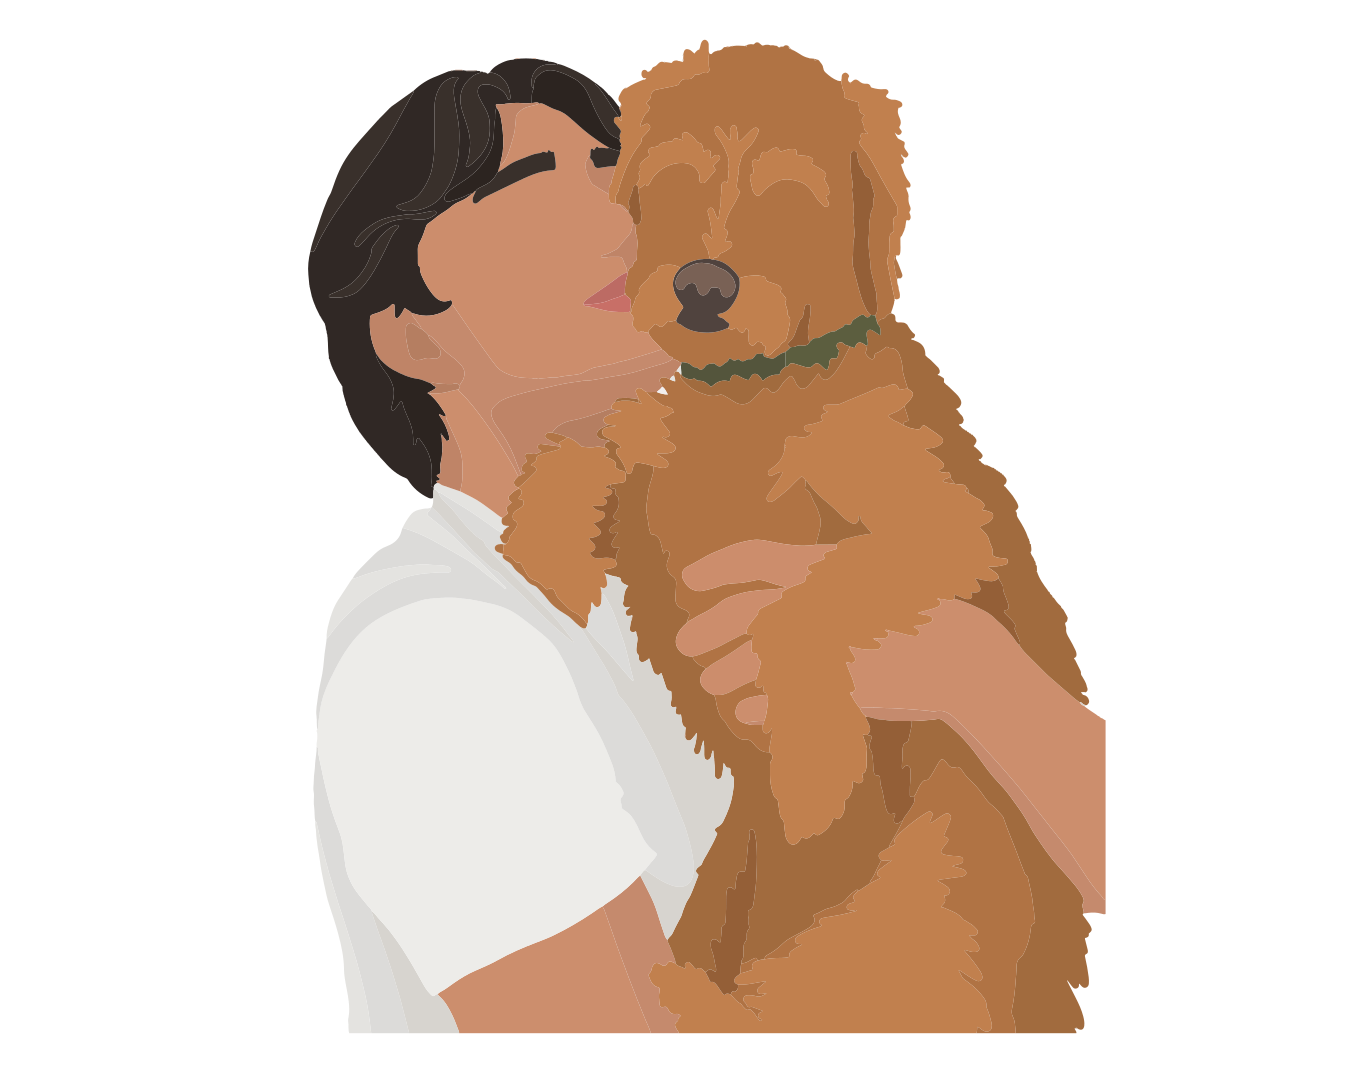
\includegraphics[width=4.16667in,height=\textheight]{chapters/00-dedication/figure/dedication_2.png}
\end{center}

\bookmarksetup{startatroot}

\chapter{Technical Introduction}\label{technical-introduction}

\section{Introduction}\label{introduction}

This section lays out the framework for the rest of the book. First we
start with the first principles defining what populations and samples
are and distinguishing them

\section{Measure-Theoretic Framework}\label{measure-theoretic-framework}

\subsection{Outcome Space and Population of
Interest}\label{outcome-space-and-population-of-interest}

Let \((\Omega,\mathcal{F}_\Omega)\) be a measurable space. The set
\(\Omega\) is the outcome space (i.e., the universe of possible
outcomes) where each \(\omega \in \Omega\) is an outcome . The
\(\sigma\)-field \(\mathcal{F}_\Omega\) is a collection of subsets of
\(\Omega\) that is closed under countably many set operations. Let
\((\Psi, \mathcal{F}_\Psi)\) be a measurable space where the set
\(\Psi\) is the population of interest where each \(\psi \in \Psi\) is
an experimental object of study such as an individual person or animal.
Throughout the text \(\psi\) will most often be referred to as an
``individual'', but take note that this encompasses any experimental
object of interest.

\begin{figure}[H]

\centering{

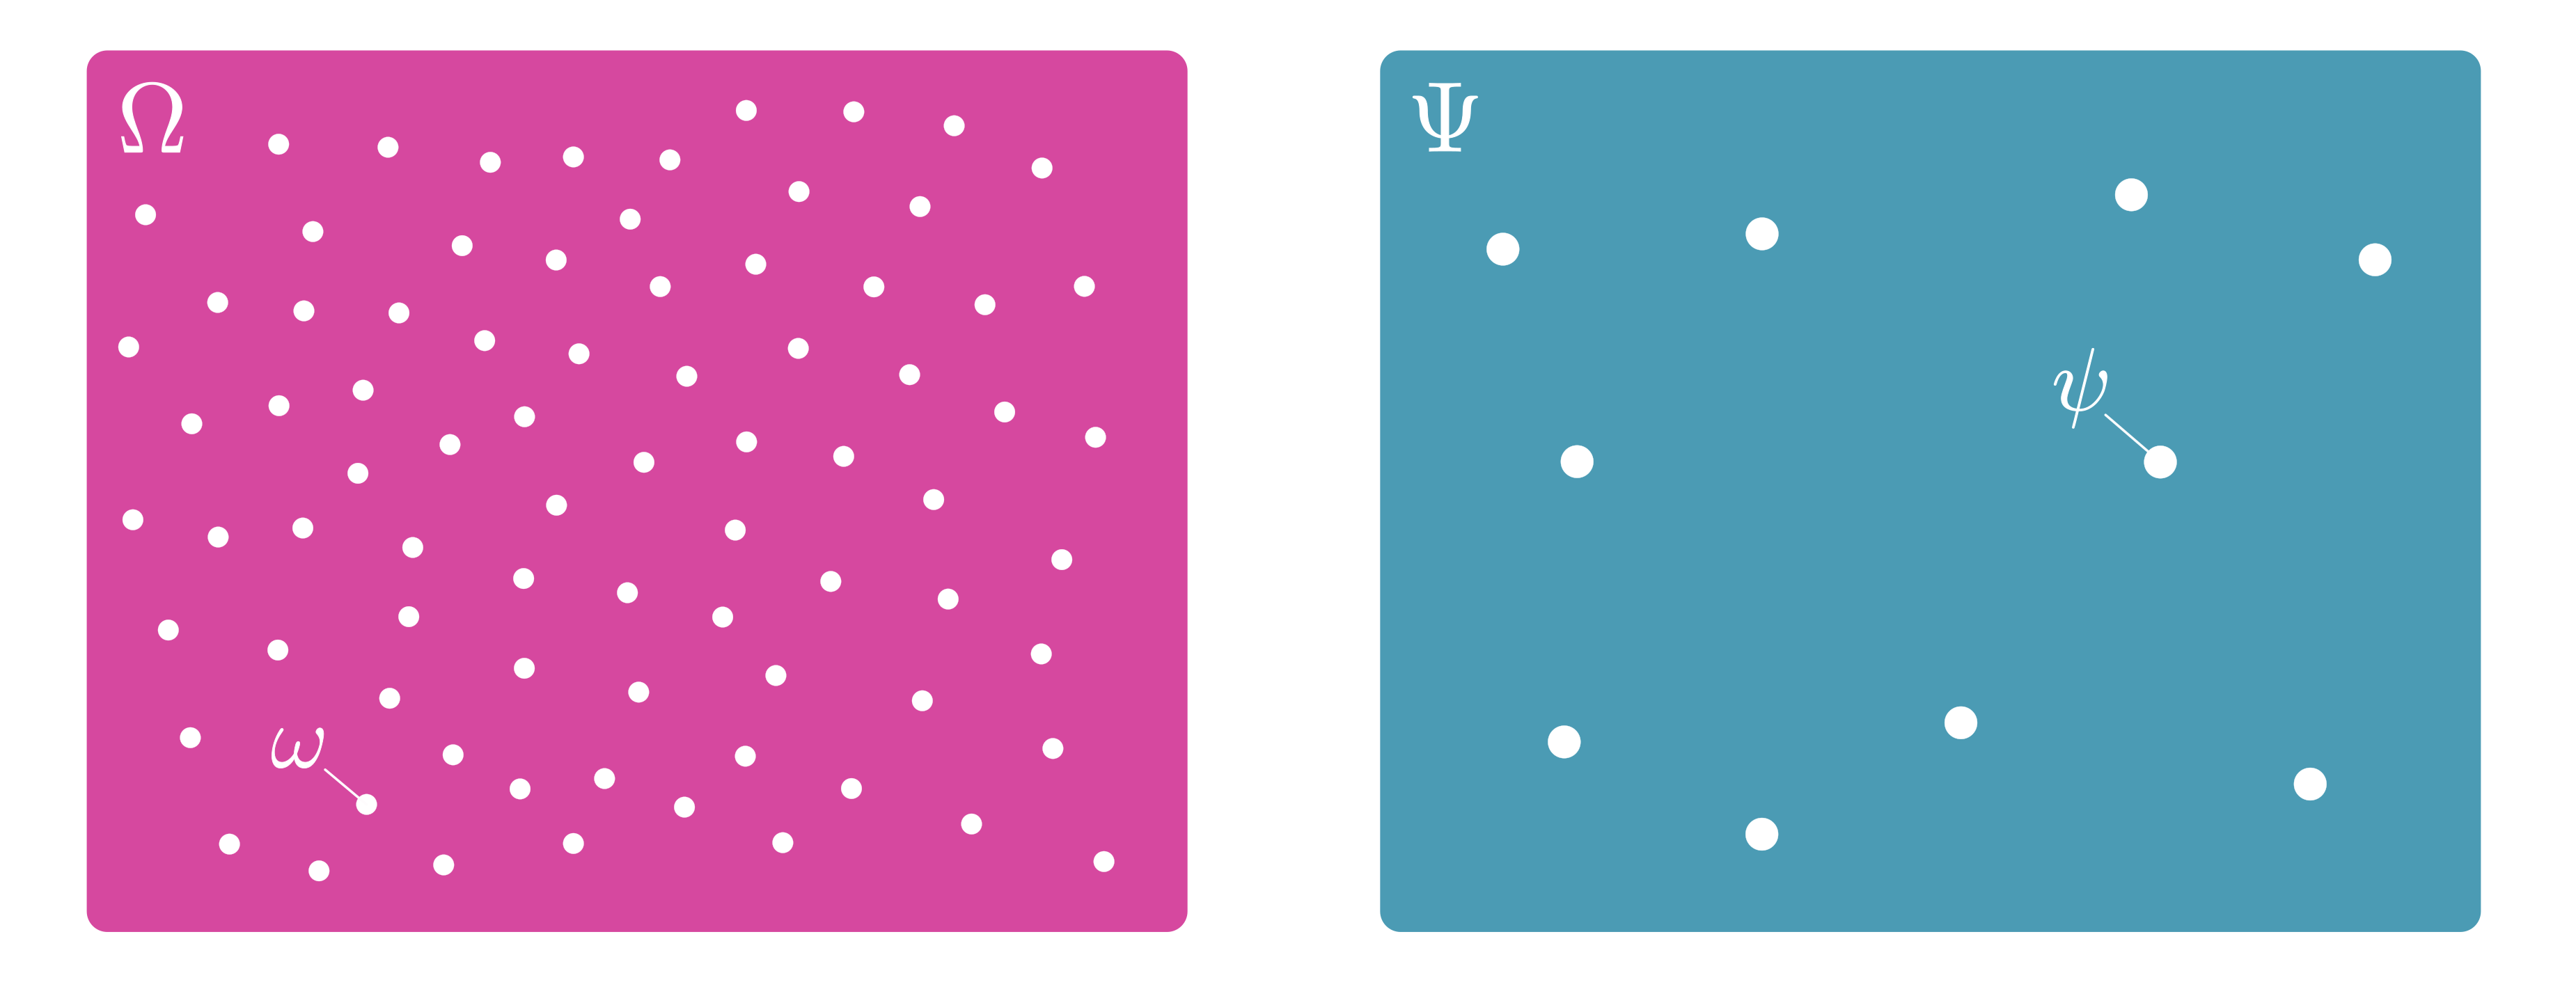
\includegraphics{chapters/01-definitions/figure/spaces.png}

}

\caption{\label{fig-spaces}Spaces \(\Omega\) and \(\Psi\). The space
\(\Omega\) is the space of all possible outcomes whereas the space
\(\Psi\) is the population of interest (i.e., the space of all possible
individuals). Each dot denotes the elements \(\omega\in\Omega\) and
\(\psi\in\Psi\).}

\end{figure}%

Let \(\ell\) be an assignment-to-individual function that maps the
outcome space \(\Omega\) to the population of interest \(\Psi\)
(Zimmerman 1975; Kroc and Zumbo 2020),

\[
\ell: (\Omega,\mathcal{F}_\Omega) \rightarrow (\Psi,\mathcal{F}_\Psi).
\]

The function \(\ell\) is \(\mathcal{F}\)-measurable such that
\(\ell^{-1}(\psi) \in \mathcal{F}_{\Omega}\). The preimage of an
individual \(\psi\in\Psi\) under the assignment-to-individual function
is also known as a \emph{fiber} and encapsulates all possible outcomes
for given individual (see Figure~\ref{fig-fibers}). The fibers of
\(\ell\) create a partition of the outcome space,

\begin{equation}\phantomsection\label{eq-sigma-field-ell}{
\Lambda :=  \{\ell^{-1}(\psi) : \psi \in \Psi\} \subset \mathcal{F}_\Omega.
}\end{equation}

The partition \(\Lambda\) allows is the collection of disjoint subsets
of \(\Omega\) uniquely assigned to each individual in the population of
interest. Note that we can union the fibers of \(\ell\) to recover the
total outcome space such that
\(\Omega = \bigcup_{\psi\in\Psi}\ell^{-1}(\psi)\).

\begin{figure}[H]

\centering{

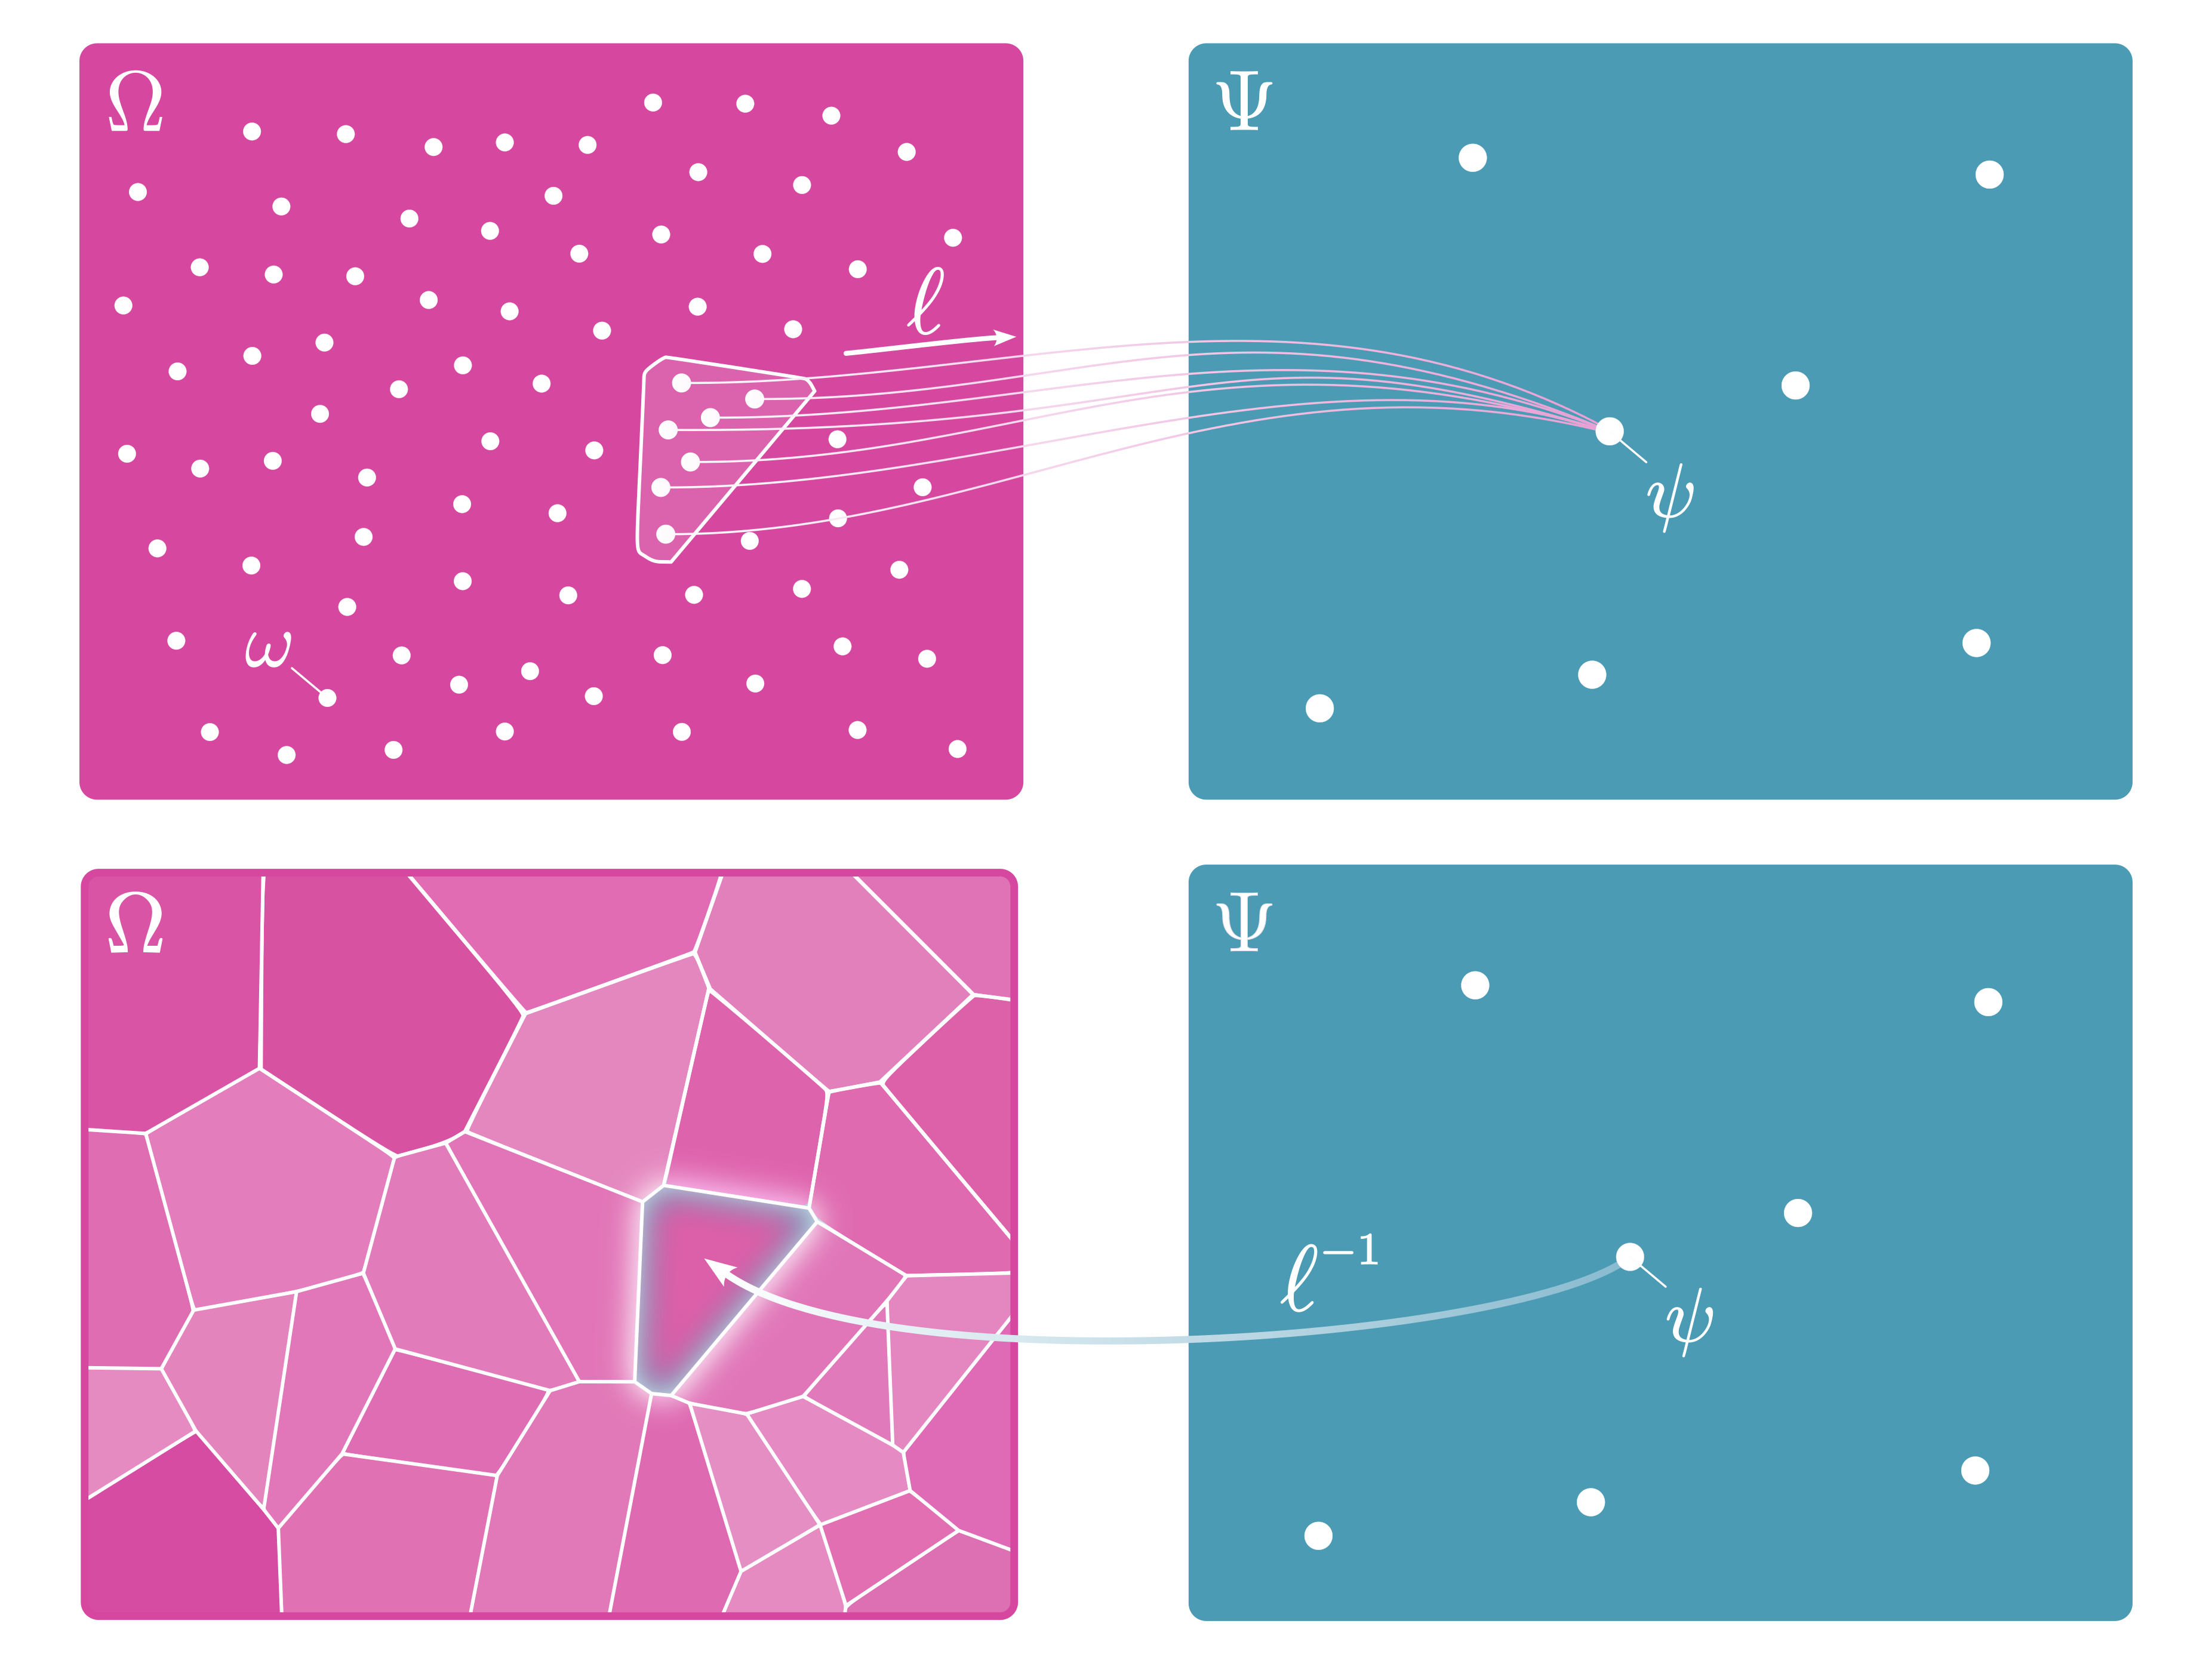
\includegraphics{chapters/01-definitions/figure/fibers.png}

}

\caption{\label{fig-fibers}Assignment-to-individual function and it's
fibers. The top panels show the function \(\ell\) mapping elements of
\(\Omega\) to a single element of \(\Psi\). The bottom panels shows a
fiber of \(\psi\) under \(\ell\) which is a subset of \(\Omega\).}

\end{figure}%

\subsection{Random Variables and Measurement
Error}\label{random-variables-and-measurement-error}

The outcomes \(\omega\) in the outcome space are arbitrary values, but
we can convert them to real number values by defining a random variable
that is a function which takes each \(\omega\in\Omega\) and assigns to
it a real-valued quantity. A real-valued random variable \(V\) is a
measurable function that maps the measurable space
\((\Omega,\mathcal{F}_\Omega)\) equipped with a probability measure
\({\Pr}_V\) to the set of real numbers equipped with the Borel
\(\sigma\)--field (i.e., the smallest \(\sigma\)--field containing all
open sets; see Figure~\ref{fig-rv}),

\[
V: (\Omega,\mathcal{F}_\Omega,{\Pr}_V) \rightarrow (\mathbb{R},\mathcal{B}_\mathbb{R}).
\]

Where the probability measure of the outcome space is
\({\Pr}_V(\Omega)=1\).

\begin{figure}[H]

\centering{

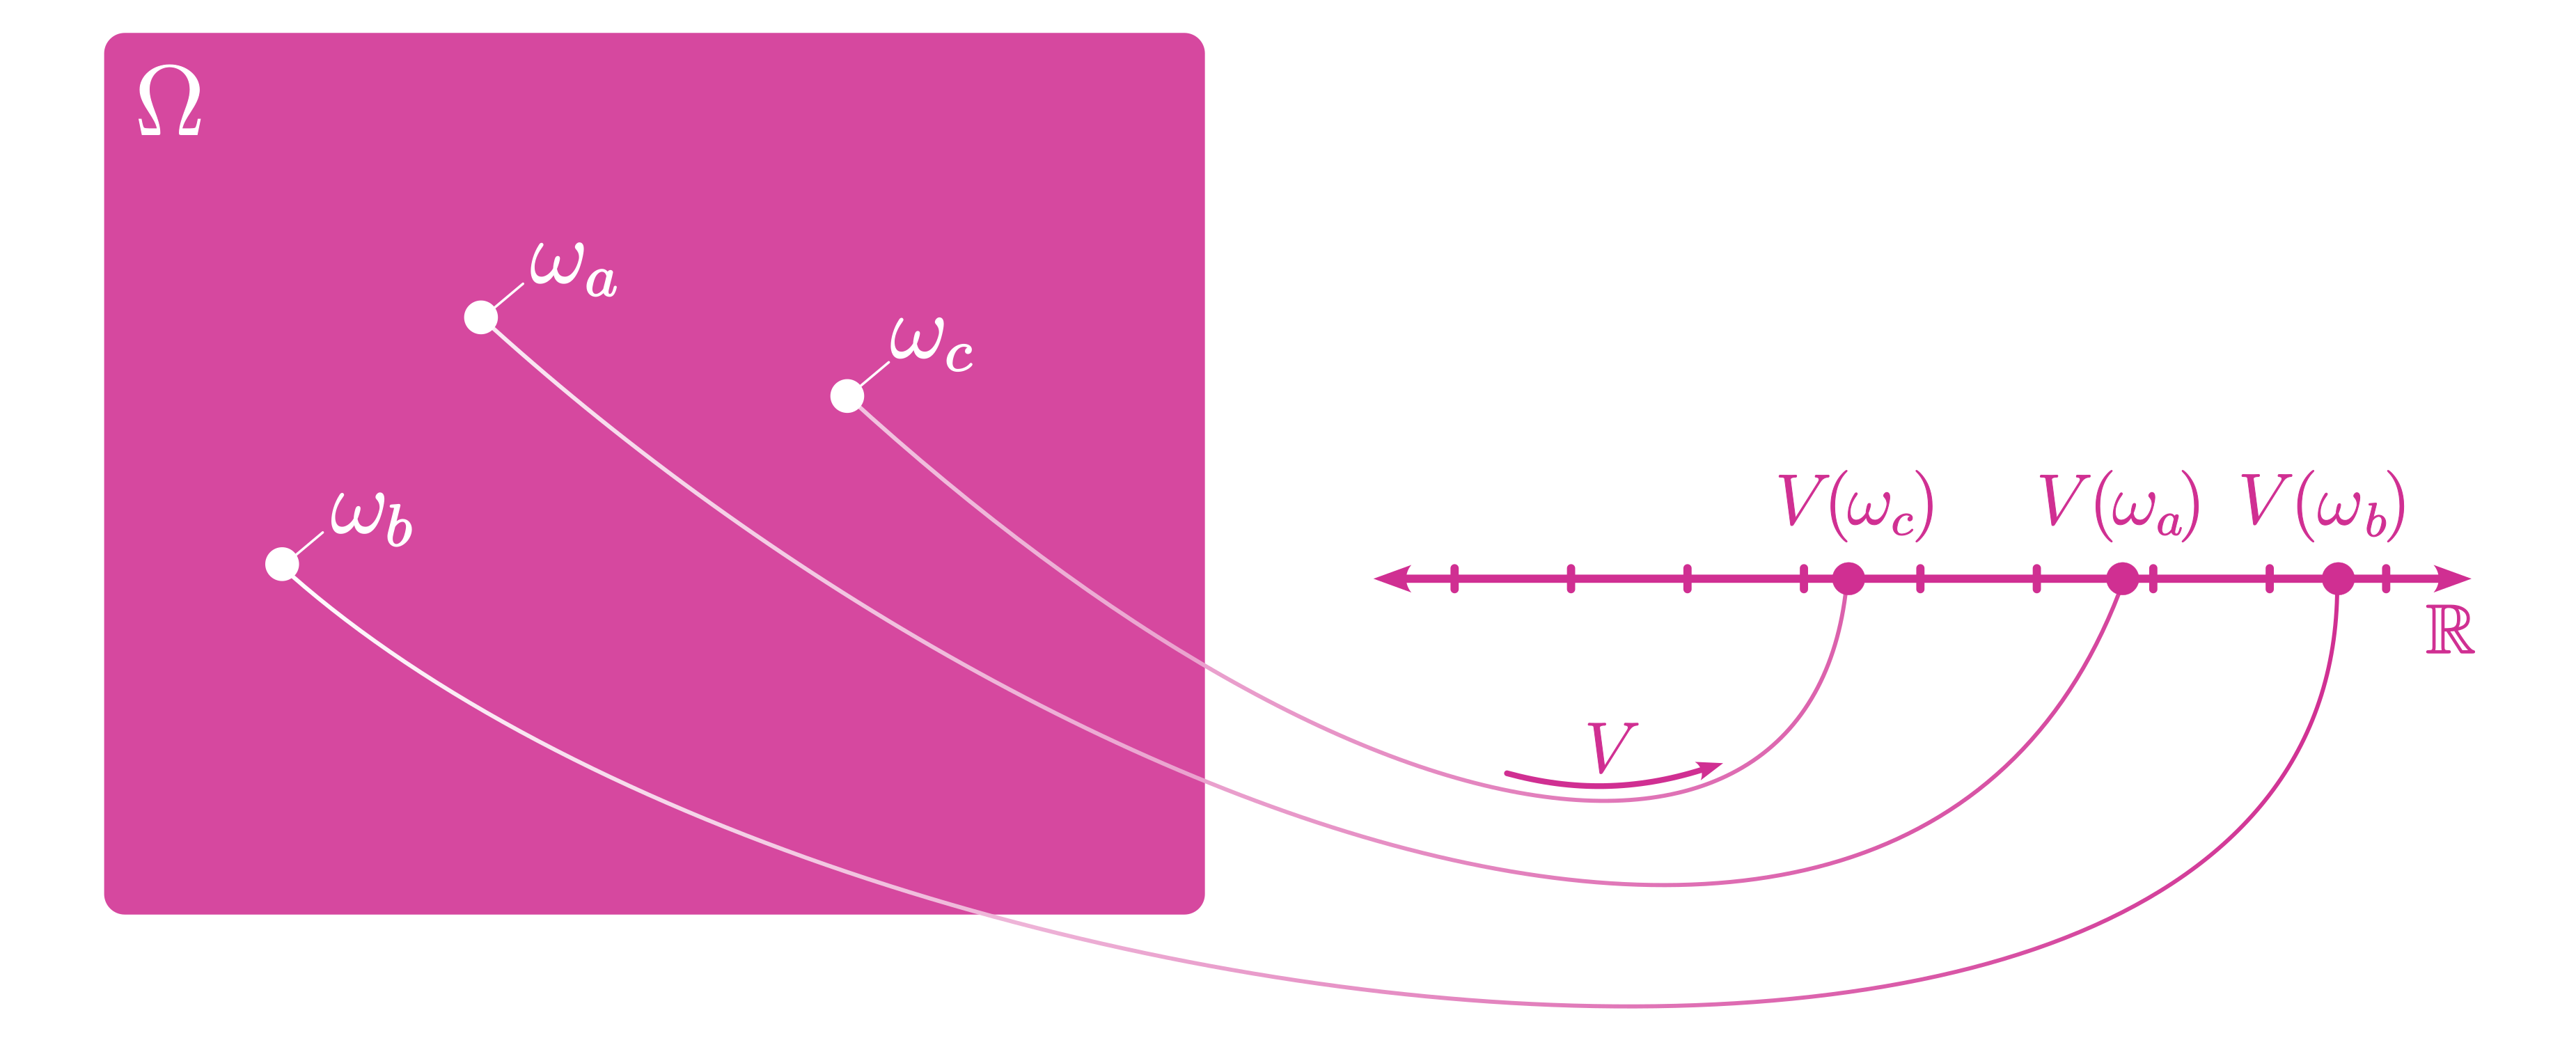
\includegraphics{chapters/01-definitions/figure/rv.png}

}

\caption{\label{fig-rv}Random variable. Three elements of \(\Omega\)
labeled \(\omega_a,\) \(\omega_b,\) and \(\omega_c\) are assigned
real-valued quantities under the random variable \(V\).}

\end{figure}%

We can now define the relevant random variables that will be used over
the course of the book. Let \(Y\) be a random variable of scientific
interest (i.e., the measurand) denoting our \emph{dependent} variable
(i.e., the outcome variable). In a study, we often need to draw
inferences about \(Y\) from an observable error-prone proxy,
\(\widetilde{Y}\). The proxy variable contains \textbf{measurement
error} which denote deviations between true value \(Y\) and values of
the proxy variable. We can specify an algebraic structure relating the
proxy \(\widetilde{Y}\) to the true value \(Y\),

\begin{equation}\phantomsection\label{eq-meas-y}{
\widetilde{Y} = Y + E_Y
}\end{equation}

Where \(E_Y\) is the measurement error term defined as the difference
between the error-prone proxy and the true value
\(E_Y = \widetilde{Y} - Y\) (see Figure~\ref{fig-me}). Let the random
variable in Equation~\ref{eq-meas-y} be continuous such that for any
outcome \(\omega\in\Omega\) the random variables take on real values
such that
\(\widetilde{Y}(\omega), Y(\omega), E_Y(\omega) \in \mathbb{R}\).

\begin{figure}[H]

\centering{

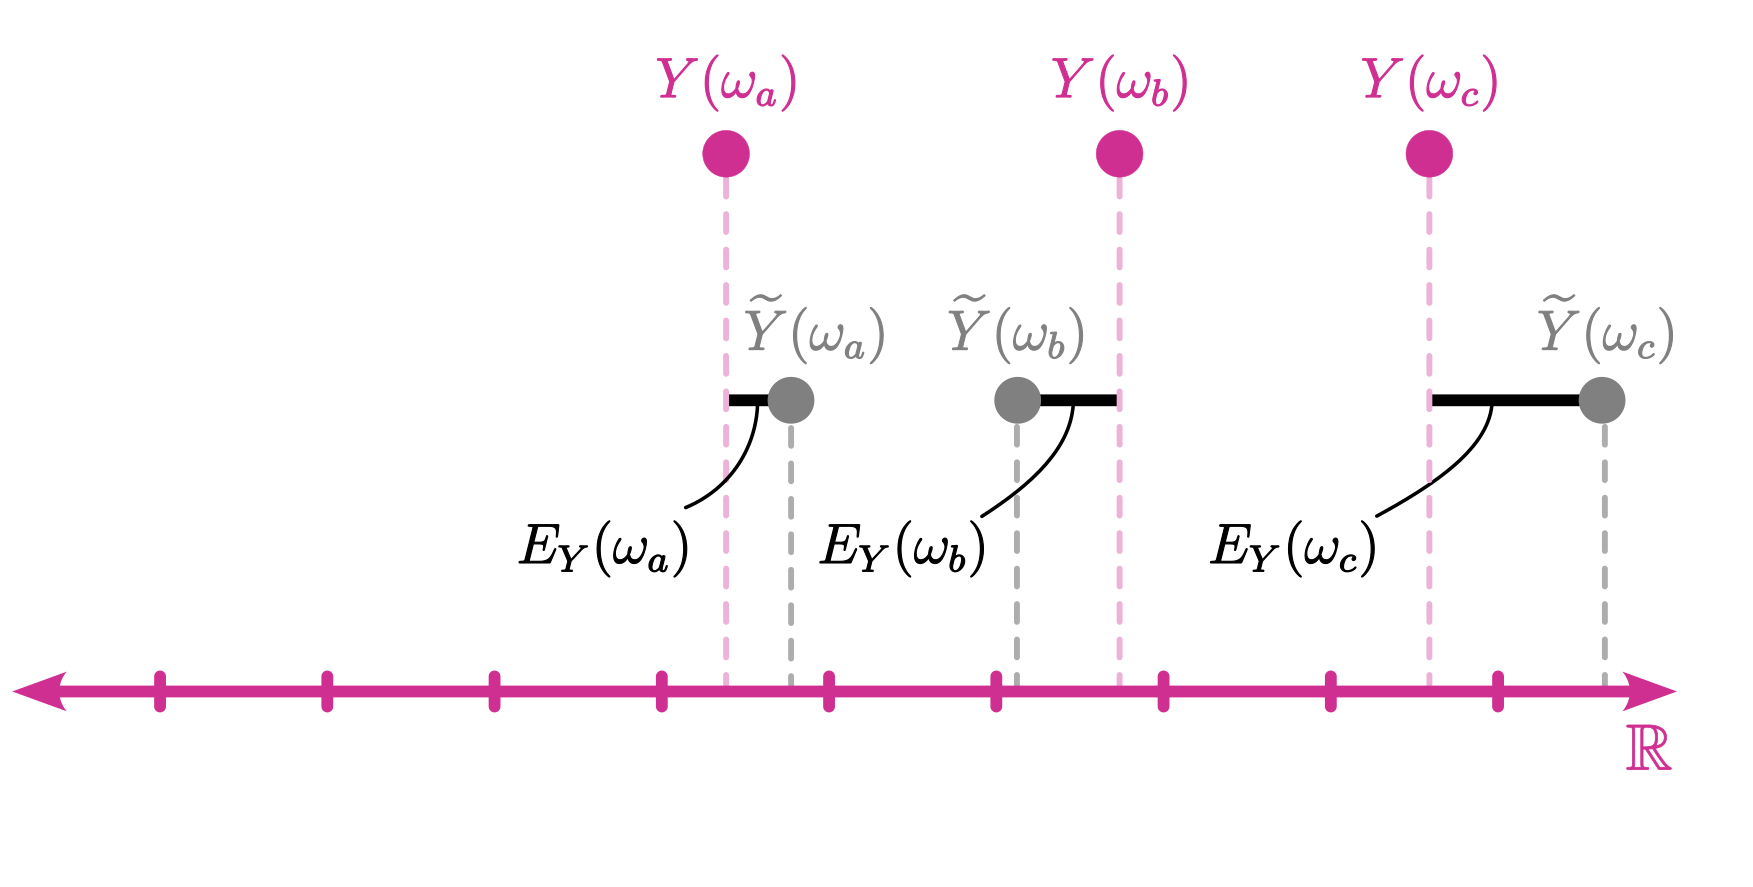
\includegraphics{chapters/01-definitions/figure/me.png}

}

\caption{\label{fig-me}Measurement error. Each of the components of
Equation~\ref{eq-meas-y} shown with respect to the real line.}

\end{figure}%

We also want to define two independent variables \(X\) and \(G\) of
interest and structure them in an algebraically similar manner to
Equation~\ref{eq-meas-y},

\begin{equation}\phantomsection\label{eq-meas-x}{
\widetilde{X} = X + E_X
}\end{equation}

\begin{equation}\phantomsection\label{eq-meas-g}{
\widetilde{G} = G + E_G
}\end{equation}

Where \(X\) is a continuous random variable such that
\(\widetilde{X}(\omega), X(\omega), E_X(\omega) \in \mathbb{R}\) and
\(G\) is a Bernoulli random variable such that
\(\widetilde{G}(\omega), G(\omega), E_G(\omega) \in\{0,1\}\). For the
sake of this book, we will would like the true value to be constant over
for each individual, that is, \(X(\omega),\) \(Y(\omega),\) and
\(G(\omega)\) is constant for all \(\omega \in \ell^{-1}(\psi)\) for
each \(\psi \in \Psi\). The error-prone proxies on the other hand will
vary within a person providing a distribution of possible values. In the
chapter on measurement error, we will define more precisely the how each
of the proxy variables are calibrated to their respective true values.

\subsection{Probability Distributions and Density
Functions}\label{probability-distributions-and-density-functions}

The probability distribution of a continuous random variable \(V\) can
be described by a probability density function \(f_V\) that satisfies,

\begin{equation}\phantomsection\label{eq-pdf-1}{
{\Pr}_V(V\in\mathbb{R}) = \int_\mathbb{R} f_V(v)\, dv = 1.
}\end{equation}

In other words, the probability of \(V\) taking on a value anywhere on
the real line is 1 (i.e., no uncertainty in that statement). To obtain
the probability that \(V\) exists in some subset
\(B \subset \mathbb{R}\) of the real line (e.g., an interval), we can
integrate the probability density function \(f_V\) over \(B\),

\begin{equation}\phantomsection\label{eq-pdf-2}{
{\Pr}_V(V\in B) = \int_{B} f_V(v)\, dv.
}\end{equation}

\begin{figure}[H]

\centering{

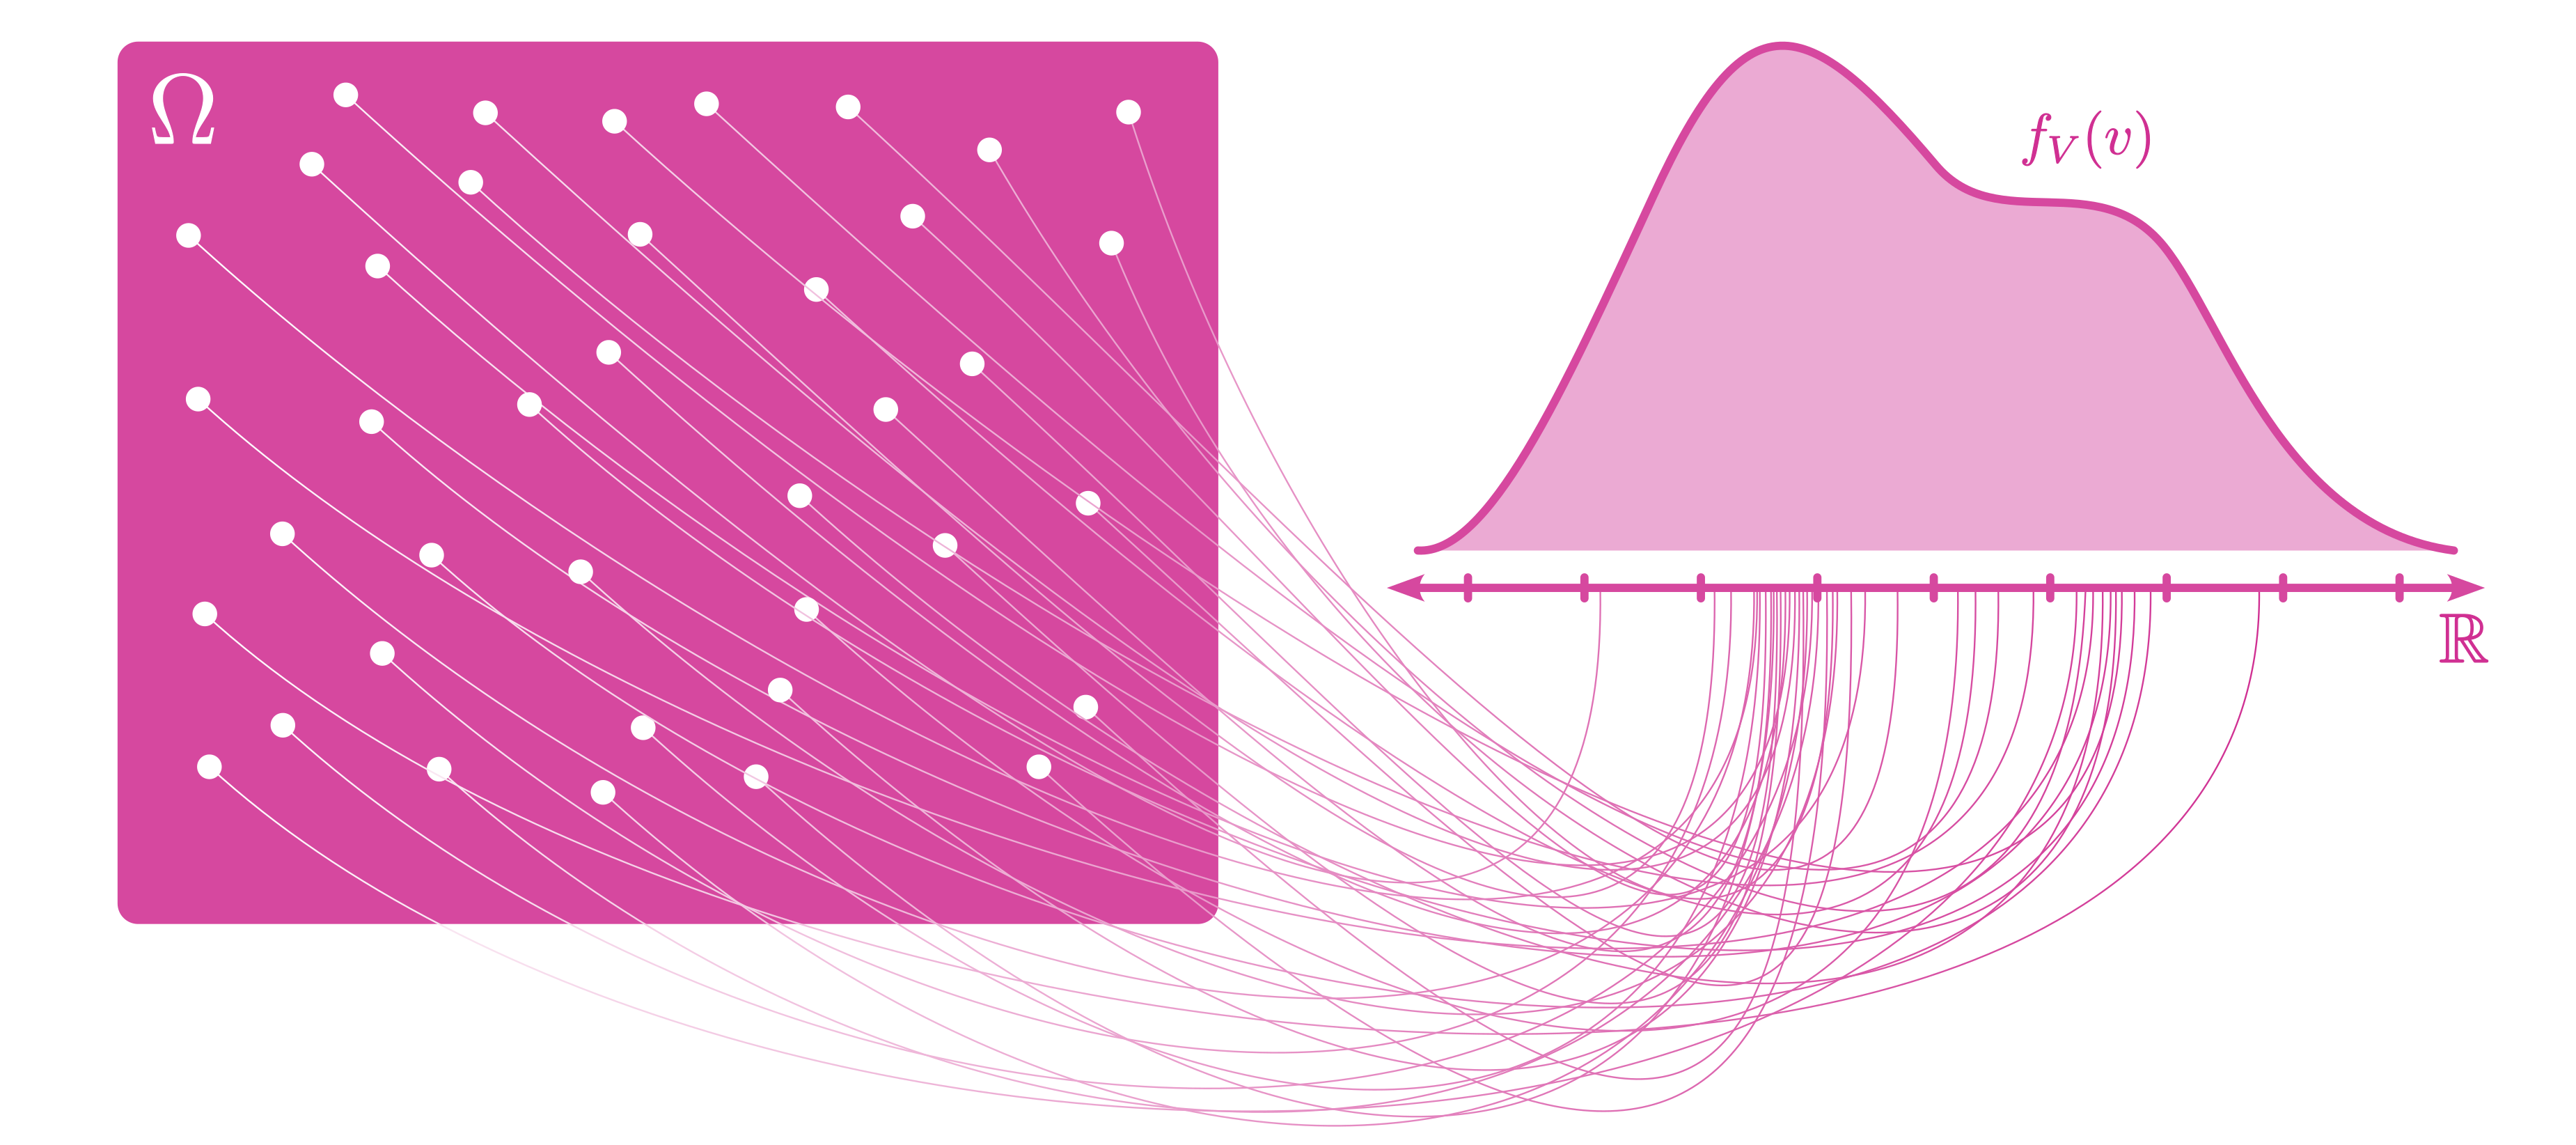
\includegraphics{chapters/01-definitions/figure/pdf.png}

}

\caption{\label{fig-pdf}Probability Distributions. The outcome space
\(\Omega\) is mapped to the real line. How the values are distributed
across the real line is described by the probability density function
\(f_{V}(v)\).}

\end{figure}%

The random variables \(X\) and \(Y\) (along with the associated proxies
and errors) are continuous and their probability distributions can both
be described by their respective probability density functions \(f_X\)
and \(f_Y\). However the Bernoulli random variable \(G\) can be
described by a probability \emph{mass} function,

\[
f_G(g) = p_G^g (1-p_G)^{1-g}
\]

Where the parameter \(p_G\) denotes the probability that \(G=1\).
Therefore the probability distribution of 0 or 1 can explicitly written
out as,

\[
{\Pr}_G(G = 1) = p_G \;\;\; \text{and} \;\;\;
{\Pr}_G(G = 0) = 1-p_G.
\]

\begin{figure}[H]

{\centering 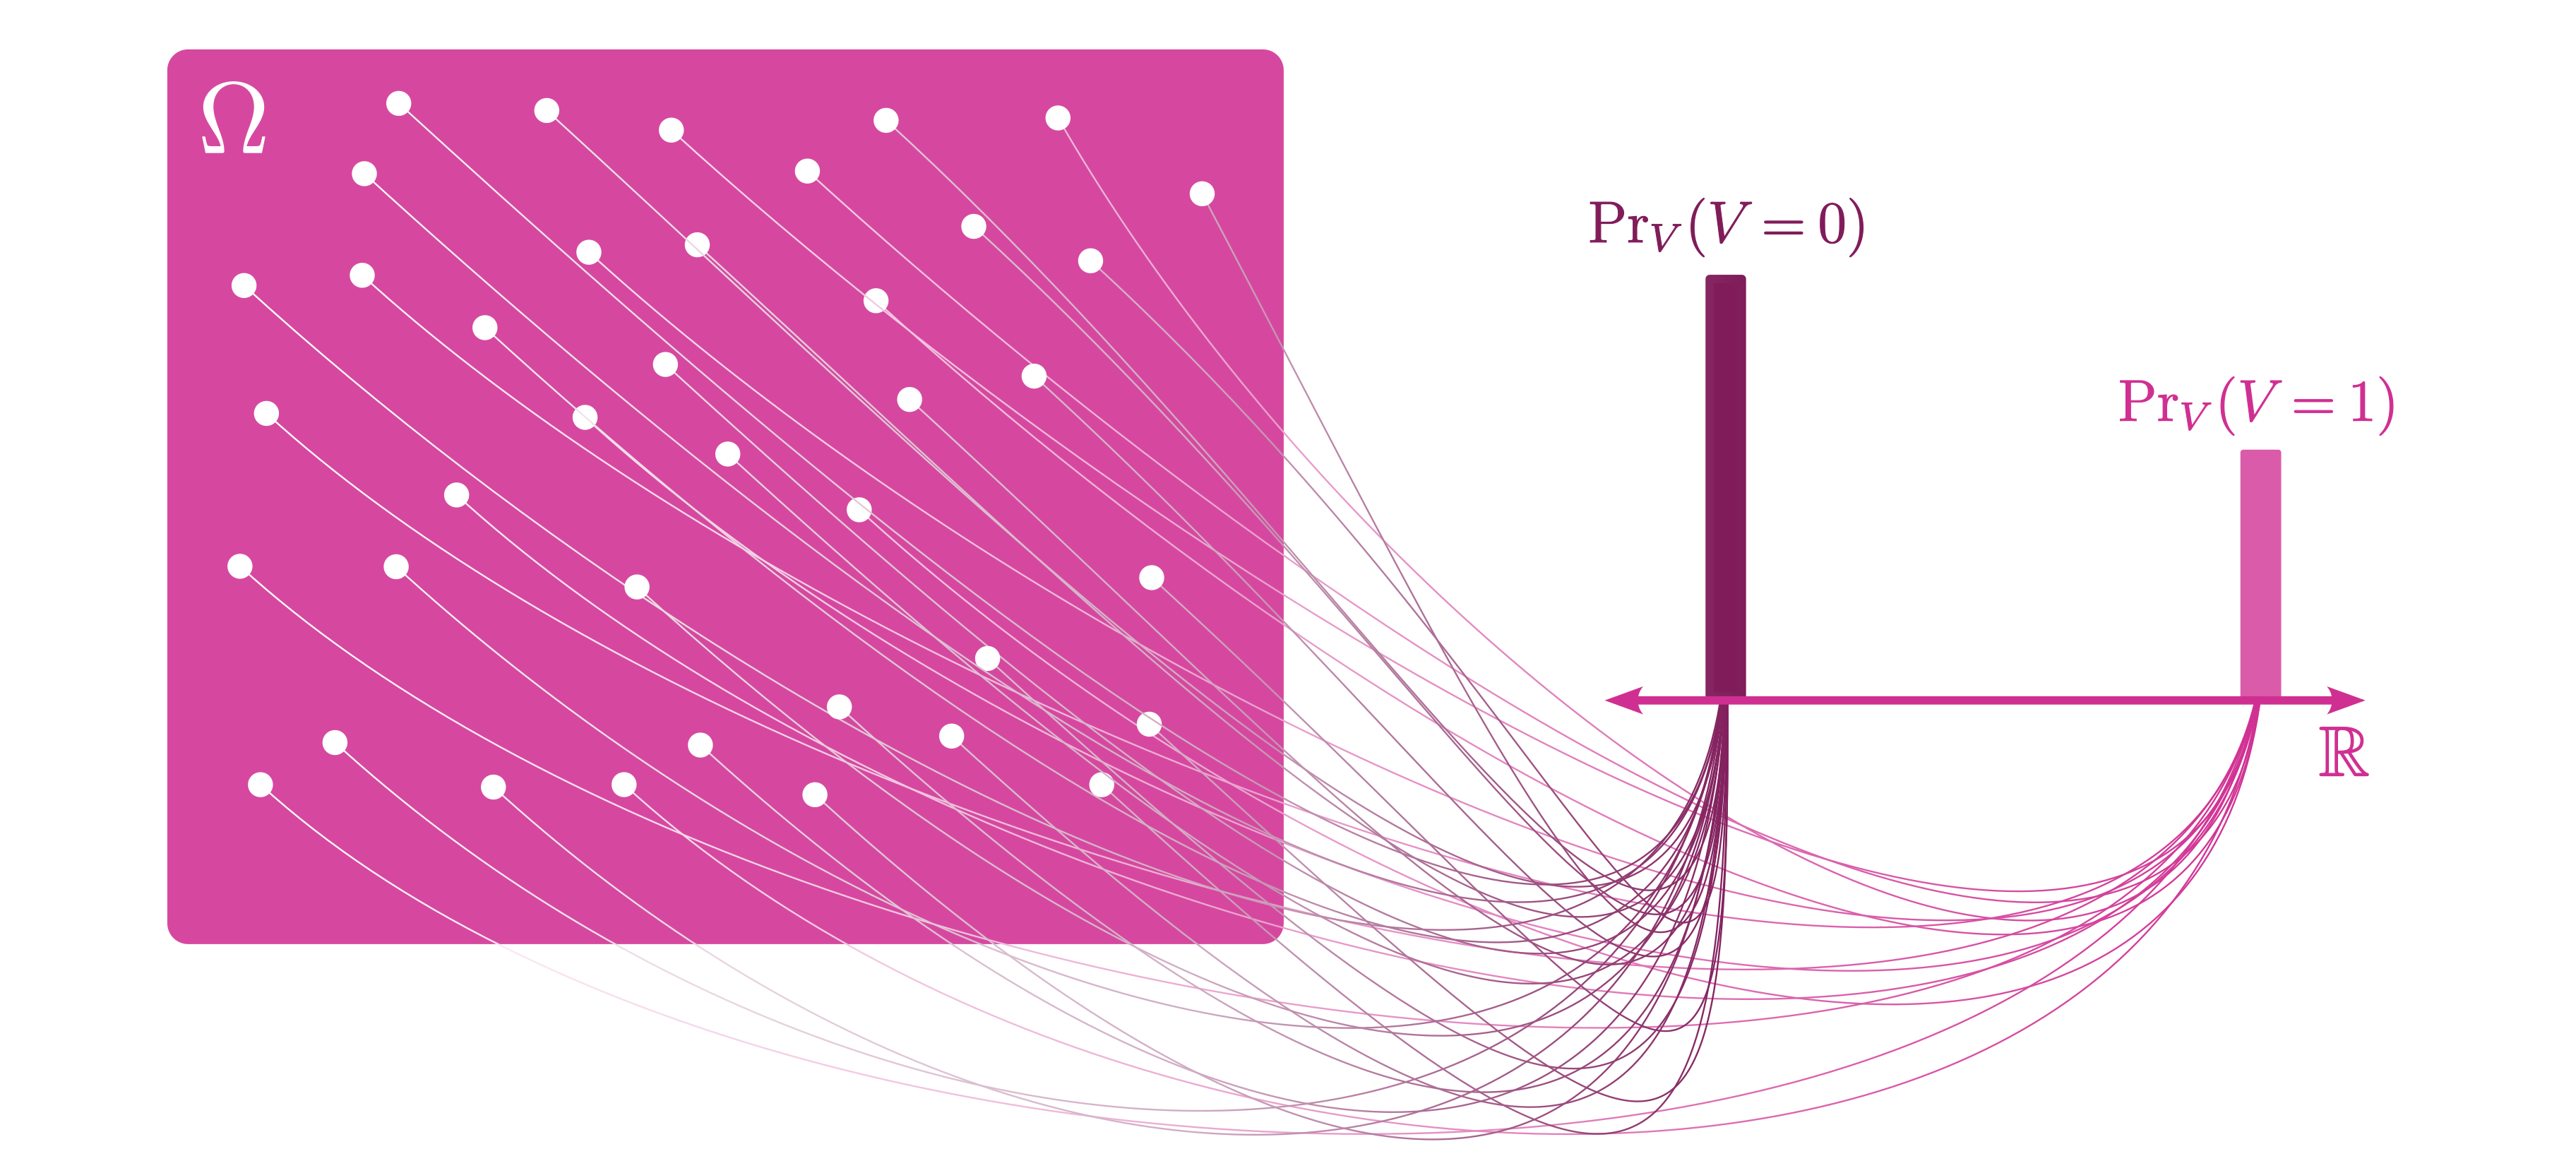
\includegraphics{chapters/01-definitions/figure/bernoulli-pdf.png}

}

\caption{Probability Distributions. The outcome space \(\Omega\) is
mapped to the real line with the value of the random variable \(V\) only
taking on values of 0 or 1.}

\end{figure}%

\subsection{Expectation and Variance of Random
Variables}\label{expectation-and-variance-of-random-variables}

The expected value (i.e., the mean) of a continuous random variable is a
probability weighted average over all possible outcomes. This can be
expressed with the integral over \(\mathbb{R}\),

\[
\mu_V := \mathbb{E}\lbrack V\rbrack  = \int_\mathbb{R} v f_V(v) \, dv. 
\]

The expected value of a Bernoulli random variable is simply
\(\mathbb{E}(G)= p_G\). The variance \(\sigma^2_V\) of a random variable
\(V\) is defined as the expected value of squared differences from the
average,

\[
\sigma^2_V := \mathbb{E}\lbrack Y^2\rbrack - \mathbb{E}\lbrack Y\rbrack^2 = \mathbb{E}\left[(Y-\mu_Y)^2\right]
\]

Where the square root of the variance, \(\sigma_V\), is the standard
deviation of \(V\).

\subsection{Joint Probability Distributions and Density
Functions}\label{joint-probability-distributions-and-density-functions}

To properly think about effect sizes we must be able to describe the
relationship between random variables. For our purposes, we want to be
able to describe the relationship between independent (\(X\),\(G\)) and
dependent variables (\(Y\)). Let's first consider the product between
two real-valued measurable spaces,

\[
(\mathbb{R},\mathcal{B}_\mathbb{R}) \times(\mathbb{R},\mathcal{B}_\mathbb{R}) = (\mathbb{R}\times \mathbb{R},\mathcal{B}_\mathbb{R} \otimes \mathcal{B}_\mathbb{R}) = (\mathbb{R}^2,\mathcal{B}_{\mathbb{R}^2}),
\]

The resulting space \((\mathbb{R}^2,\mathcal{B}_{\mathbb{R}^2})\) is a
\emph{product} space where \(\mathcal{B}_{\mathbb{R}^2}\) is the Borel
\(\sigma\)--field over \(\mathbb{R}^2\). Notice that the product of two
copies of the Borel \(\sigma\)--field over \(\mathbb{R}\) is equal to
the Borel \(\sigma\)--field over \(\mathbb{R}^2\). The independent
random variables \(X\) and \(G\) and the dependent random variables
\(X\) and \(Y\) map the outcome space equipped with a joint probability
measure to the real-valued product space,

\[
(X,Y) : (\Omega, \mathcal{F}_{\Omega},{\Pr}_{XY}) \rightarrow  (\mathbb{R}^2,\mathcal{B}_{\mathbb{R}^2}).
\]

\[
(G,Y) : (\Omega, \mathcal{F}_{\Omega},{\Pr}_{GY}) \rightarrow  (\mathbb{R}^2,\mathcal{B}_{\mathbb{R}^2}).
\]

Therefore the image of \((X,Y)\) and \((G,Y)\) is

\[
(X,Y)(\omega) = (X(\omega),Y(\omega)) \in \mathbb{R}^2,
\]

\[
(G,Y)(\omega) = (G(\omega),Y(\omega)) \in \{0,1\}\times\mathbb{R}.
\]

\begin{figure}[H]

\centering{

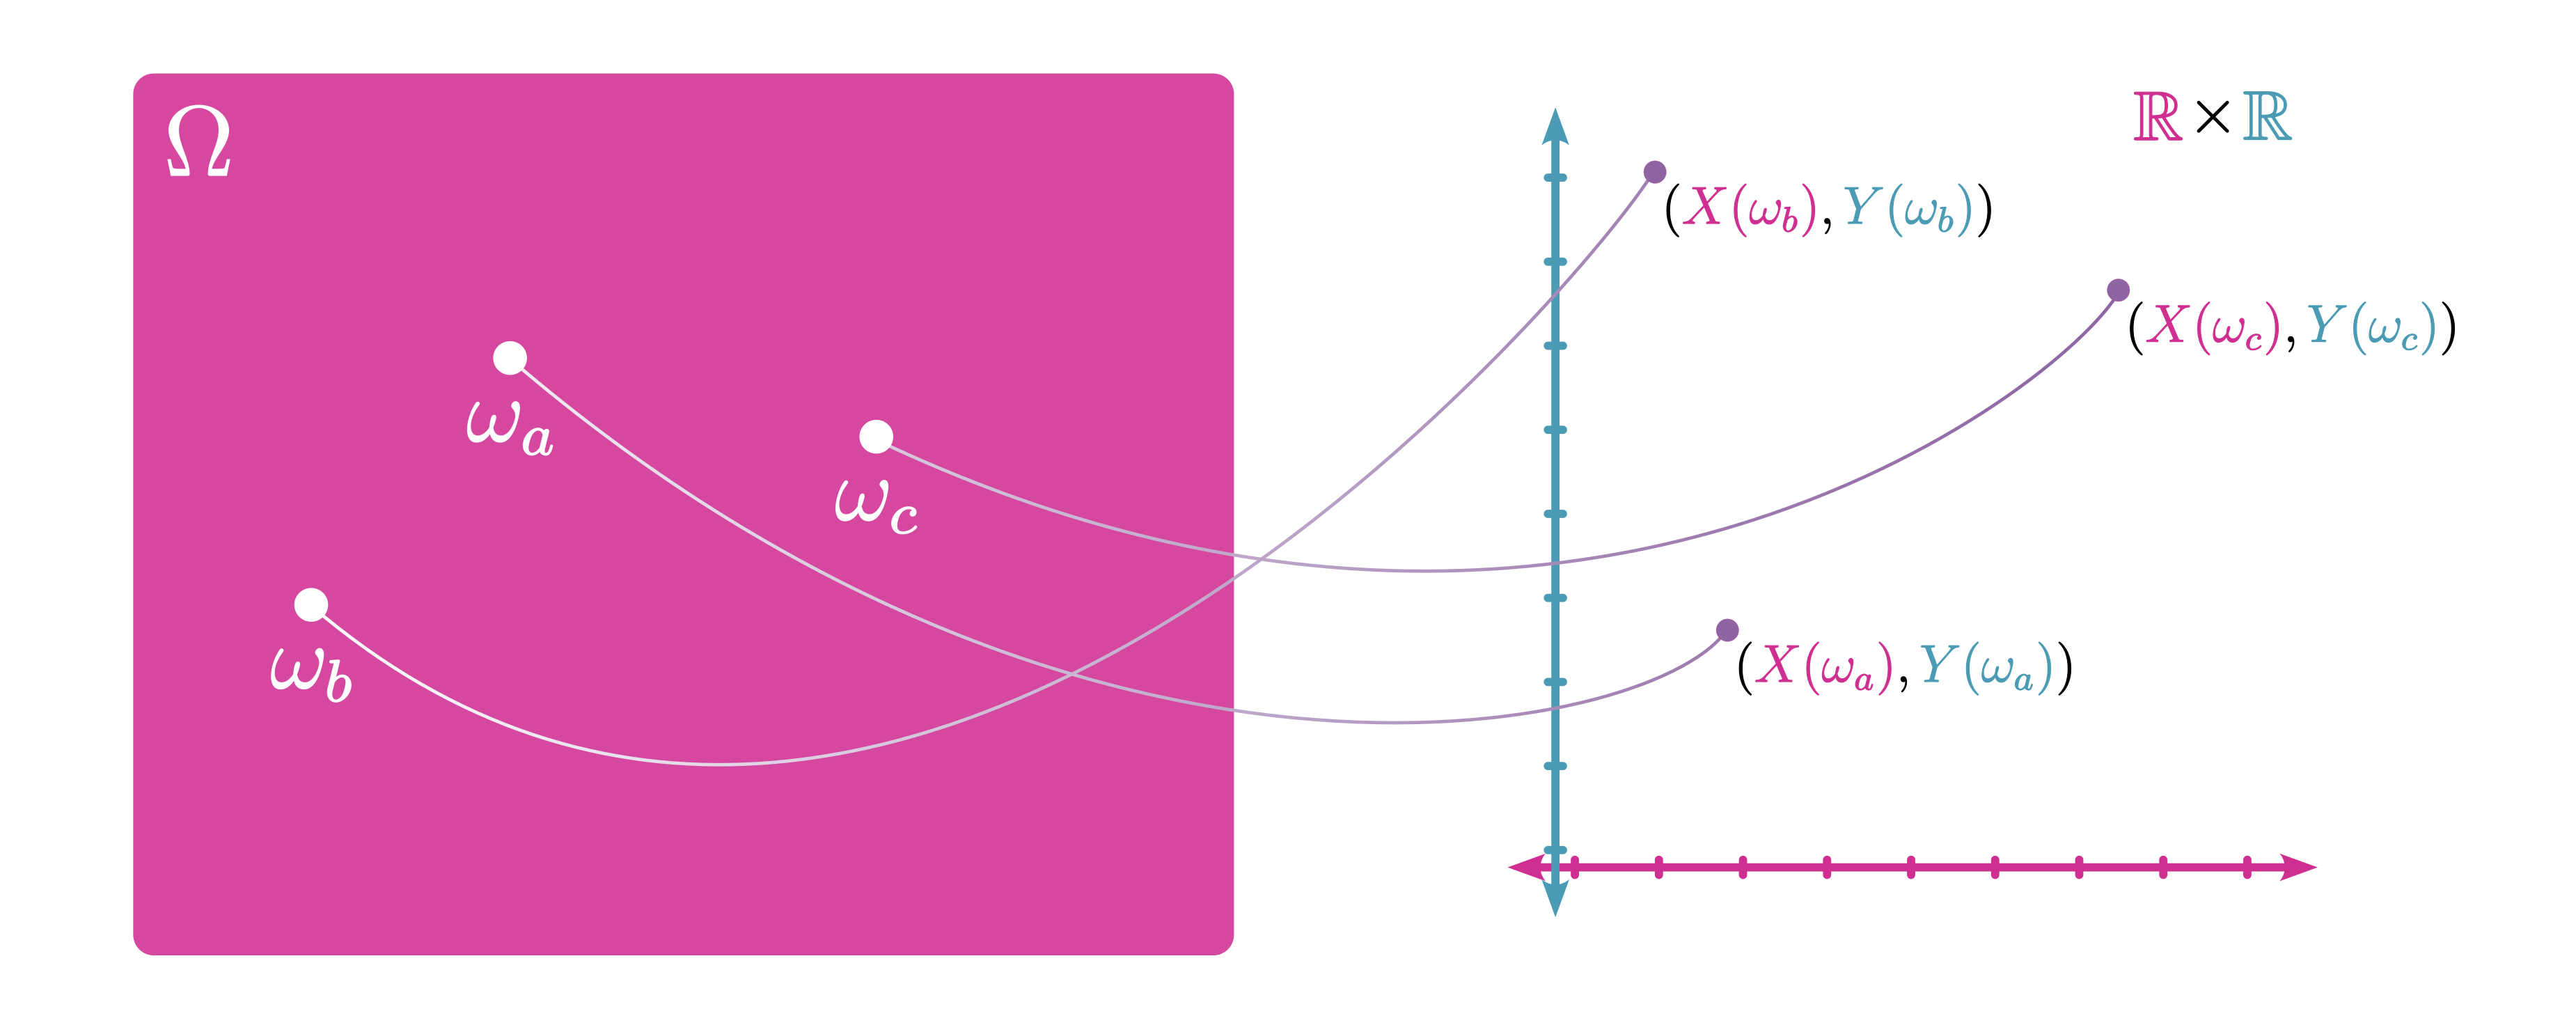
\includegraphics{chapters/01-definitions/figure/biv rv.png}

}

\caption{\label{fig-biv-rv}Random variables on product spaces. The
random variables \((X,Y)\) take on values in \(\mathbb{R}^2\).}

\end{figure}%

The probability distributions of each pair of random variables can now
be considered jointly. Joint probability distributions between can be
described by joint density functions \(f_{XY}\) and \(f_{GY}\) that
satisfies,

\[
{\Pr}_{XY}(X,Y \in \mathbb{R}^2) = \iint\limits_{\mathbb{R}^2} f_{XY}(x,y) \,dx \, dy  = 1.
\]

\[
{\Pr}_{GY}(G,Y \in \mathbb{R}^2) = \iint\limits_{\mathbb{R}^2} f_{GY}(g,y) \,dg \, dy  = 1.
\]

The probability of \(X,Y\in B\) for any set
\(B\in\mathcal{B}_{\mathbb{R}^2}\) can be expressed similarly,

\[
{\Pr}_{XY}(X,Y \in B) = \iint\limits_{B} f_{XY}(x,y) \,dx \, dy.
\] \[
{\Pr}_{GY}(G,Y \in B) = \iint\limits_{B} f_{GY}(g,y) \,dg \, dy.
\]

The distribution is visualized in \textbf{?@fig-jointpdf}

\begin{figure}[H]

\centering{

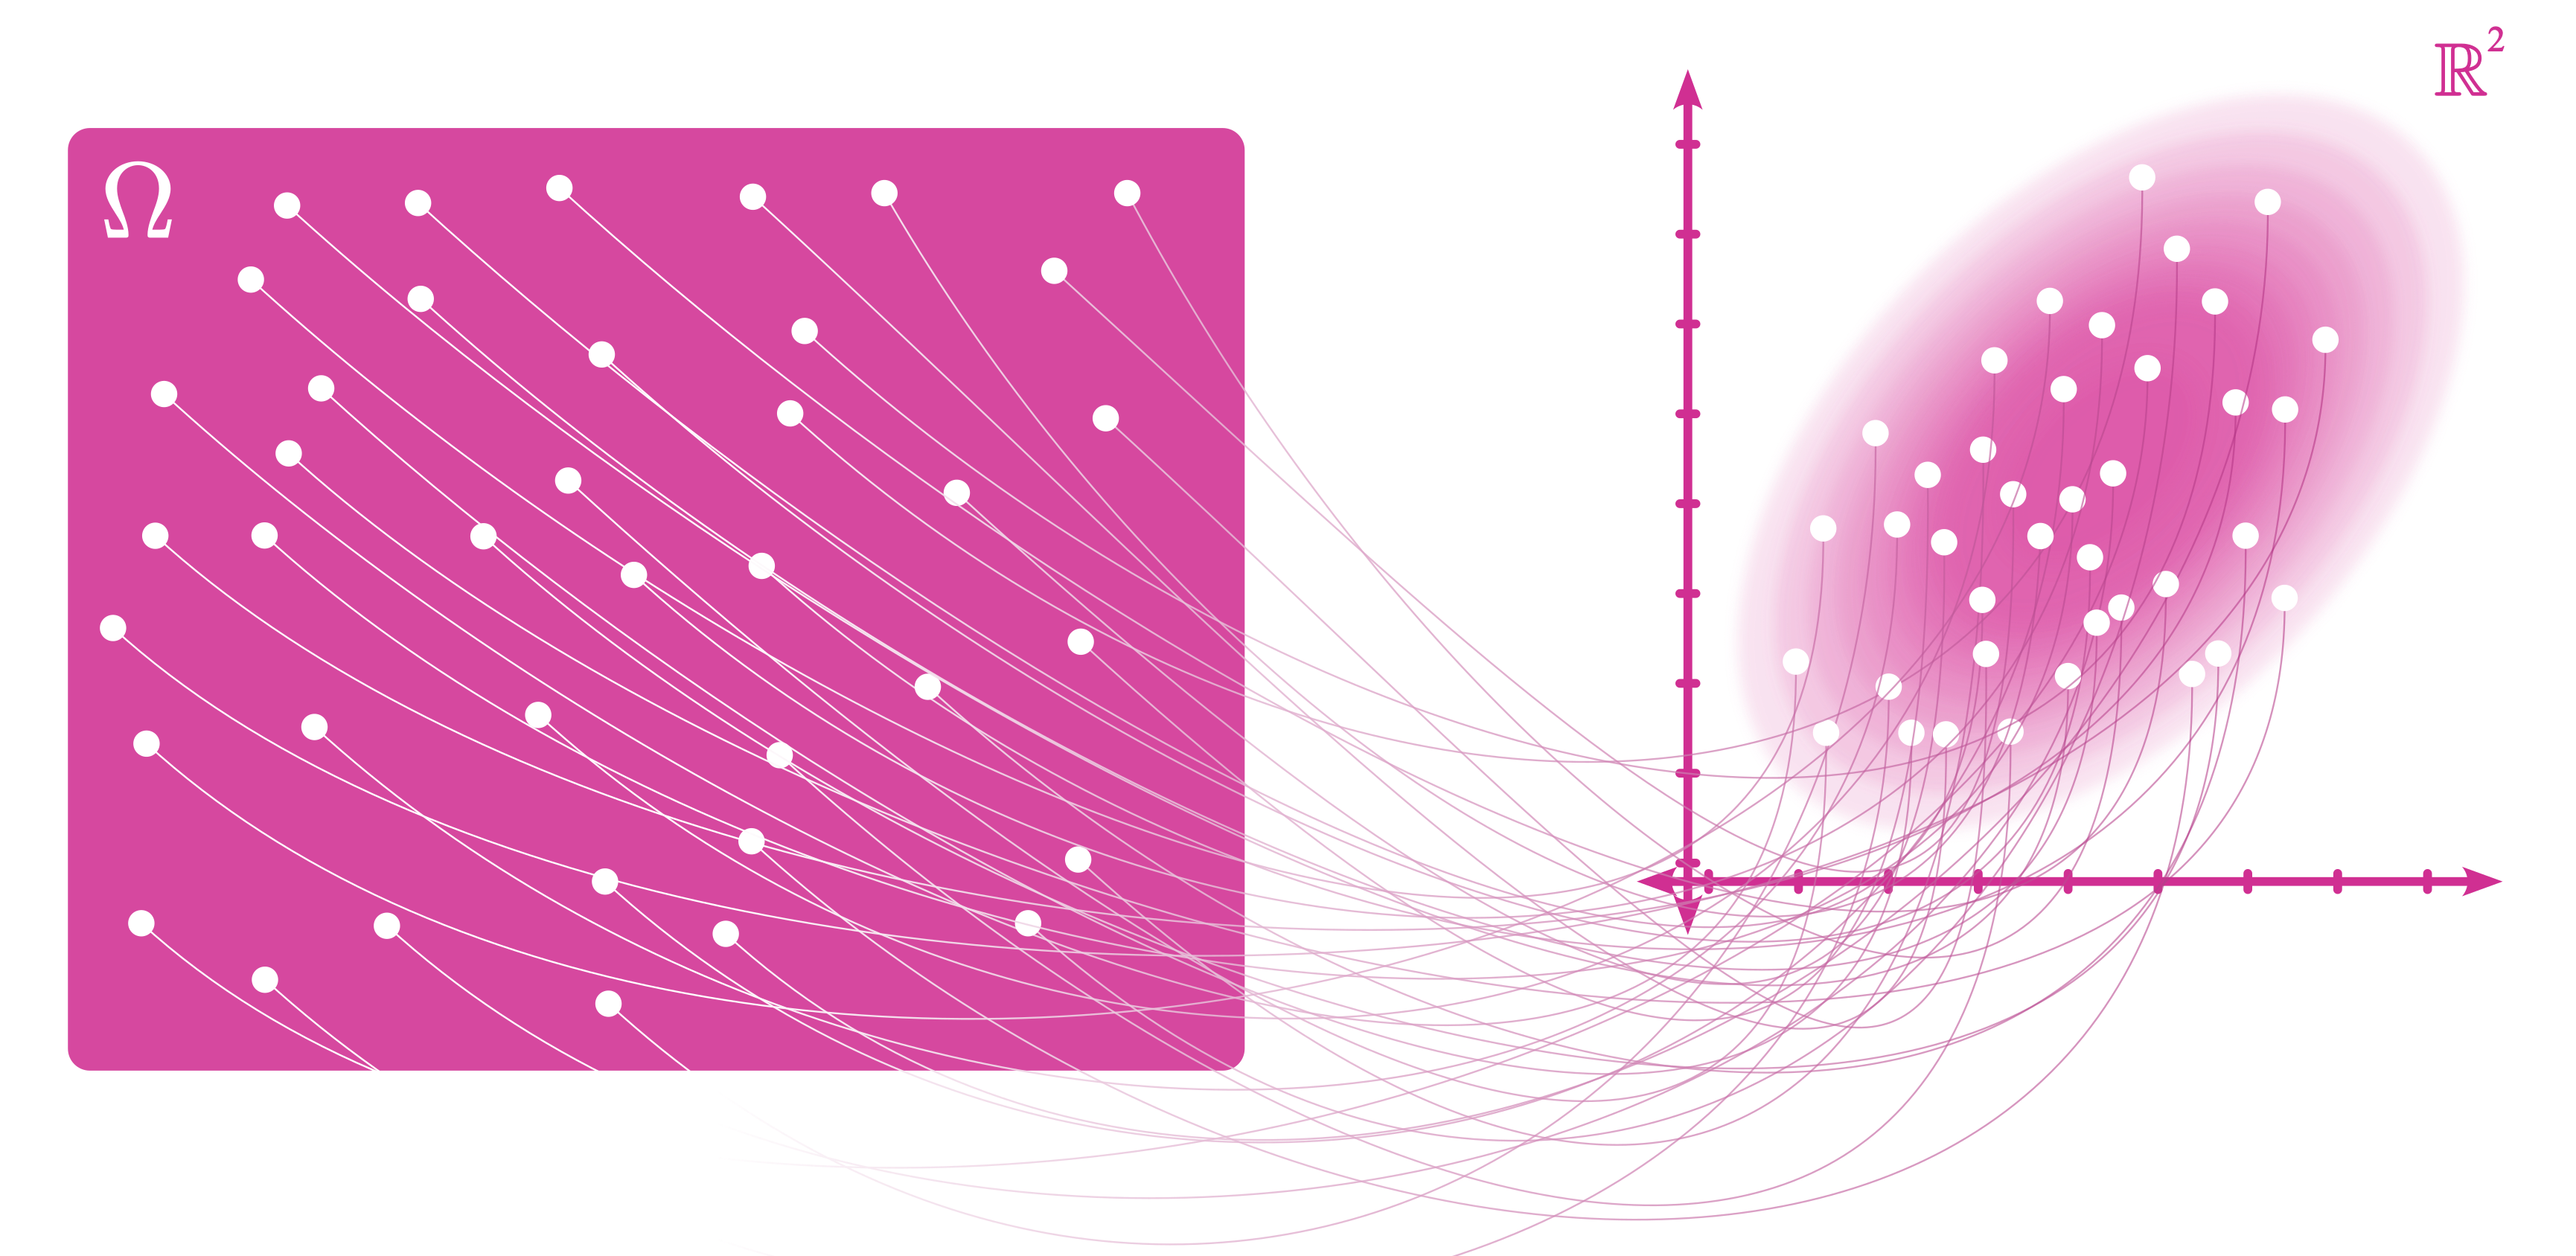
\includegraphics{chapters/01-definitions/figure/biv-joint.png}

}

\caption{\label{fig-joint-pdf}Joint distributions. The joint
distribution of \((X,Y)\). Shaded areas in the product space denotes the
probability density with darker pink denotes higher density.}

\end{figure}%

\subsection{Conditional Expectations and
Variance}\label{conditional-expectations-and-variance}

Importantly, the joint density can be used to obtain the conditional
expectation and variance. For instance, we can calculate the expected
value of \(Y\) given \(G=1\) using the joint density \(f_{GY}\),

\begin{equation}\phantomsection\label{eq-cond-mean}{\begin{align}
\mu_{Y|G=1} :=& \mathbb{E}\lbrack Y \mid G=1\rbrack \\=& \frac{1}{f_G(G=1)}\int_{\mathbb{R}} y\, f_{GY}(G=1,y) \, dy,
\end{align}}\end{equation}

where the term \(\frac{1}{f_G(G=1)}\) is used for renormalizing the
probability density function. The conditional variance is,

\begin{equation}\phantomsection\label{eq-cond-var}{\begin{align}
\sigma^2_{Y|G=1} :=& \mathbb{E}\lbrack Y^2 \mid G=1\rbrack - \mathbb{E}\lbrack Y \mid G=1\rbrack^2\\ =& \mathbb{E}\left[(Y_{G=1}-\mu_{Y|G=1})^2\right].
\end{align}}\end{equation}

We can also define the \textbf{covariance} between two variables as the
expected value of the product of the differences from the mean,

\begin{equation}\phantomsection\label{eq-cov}{\begin{align}
\sigma_{XY} = \mathbb{E}\lbrack XY \rbrack - \mathbb{E}\lbrack X\rbrack\mathbb{E}\lbrack Y\rbrack = \mathbb{E}\left[(X-\mu_X)(Y-\mu_Y)\right]
\end{align}}\end{equation}

\subsection{Effect Sizes}\label{effect-sizes}

An \textbf{effect size} is a parameter that describes the association of
two random variables\footnote{1: Effect sizes can be defined more
  broadly as the association between multiple variables, however this
  book will only focus on the more narrow case of just two variables.}
(e.g., \(X\) and \(Y\)). Effect sizes are often used to quantify
scientific research findings and are usually the target quantity in a
research study. Using expected values, we can define two types of effect
sizes that will be of primary focus throughout the book: correlations
and standardized mean differences. A \textbf{correlation} can be defined
as the standardized covariance between two variables. For two continuous
random variables, \(X\) and \(Y\), the correlation \(\rho_{XY}\) can be
expressed as,

\begin{equation}\phantomsection\label{eq-pop-corr}{
\rho_{XY} = \frac{\sigma_{XY}}{\sigma_X\sigma_Y}.
}\end{equation}

However a correlation does not have to be between two continuous
variables. Typically a correlation between a Bernoulli random variable
and a continuous random variable is a \emph{point-biserial} correlation
and it is expressed similarly to Equation~\ref{eq-pop-corr},

\begin{equation}\phantomsection\label{eq-pb-corr}{
\rho_{GY} := \frac{\sigma_{GY}}{\sigma_G\sigma_Y}.
}\end{equation}

The correlation coefficient is a bounded by -1 and 1The relationship
between a Bernoulli random variable and a continuous random variable can
alternatively be expressed as a standardized mean difference. A
\textbf{standardized mean difference} is the mean difference between two
groups standardized by the within-group standard deviation. The groups
are defined by the Bernoulli random variable and the standardized mean
difference,

\begin{equation}\phantomsection\label{eq-pop-smd}{
\delta_{GY} :=  \frac{\mu_{Y|G=1}-\mu_{Y|G=0}}{\sigma_{Y|G}}.
}\end{equation}

Note that this formulation assumes homogeneity of variances between
groups such that, \(\sigma_{Y|G}=\sigma_{Y|G=1}=\sigma_{Y|G=0}\). The
effect sizes can also be functions of error-prone proxies of each of
these variables (e.g., \(\rho_{\widetilde{X}\widetilde{Y}}\),
\(\delta_{\widetilde{G}\widetilde{Y}}\)).

For a researcher to make inferences about effect size parameters in the
population of interest, they must draw a sample of individuals from the
population. Ideally, sampling is done at random in order to produce
unbiased estimates of the population effect size. In practice however,
this is usually not possible. In cognitive and behavioral sciences, many
studies are conducted on convenience samples that are sampled from a
narrow subset of the population of interest. A non-random sample may not
(on average) share the same composition of characteristics as the
population of interest and thus may produce biased estimates of
population effect size. Here we define a \textbf{study sample}
\(\mathcal{S}\) as a random sample of \emph{eligible} individuals, that
is, individuals that the researcher has access to. The pool of eligible
individuals \(\Psi_\mathsf{E}\) (i.e., the study population) is a subset
of the population of interest \(\Psi\), therefore an eligible individual
is any \(\psi\in\Psi_\mathsf{E} \subseteq \Psi\). The study sample
\(\mathcal{S}\) is a random draw of \(n\) eligible individuals from the
population of interest,

\[
\mathcal{S} := \{\psi_i \mid  \psi_{1}\dots\psi_n \in_\text{R} \Psi_\mathsf{E} \subseteq \Psi\},
\]

where \(\in_\text{R}\) denotes a random draw from a set. The effect size
in the population of interest is a fixed value that does not change from
sample to sample. However, an estimate of the effect size from sample
data will vary from sample to sample. We will denote sample estimates of
effect sizes with English letters as opposed to the Greek letters we
used for population effect sizes. The sample estimate of a correlation
is computed via Pearson's estimator (Pearson 1895),

\[
r_{XY} := \frac{s_{XY}}{s_{X}s_{Y}} = \frac{\sum_{i=1}^n (X_i - m_{X})(Y_i - m_{Y})}{\sqrt{\sum_{i=1}^n (X_i - m_{X})^2}\sqrt{\sum_{i=1}^n (Y_i - m_{Y})^2}},
\] \{\#eq-\}

Where \(m\) denote \(s^2\) the sample estimates of the means and
(co-)variances. For an SMD, we can use Cohen's estimator (Cohen 1988),

\[
d_{GY} = \frac{m_{Y|G=1} - m_{Y|G=0}}{s_{Y|G}} 
\]

Where the sample estimate of the standard deviation of \(Y\) given \(G\)
is the pooled within-group standard deviation,

\[
s_{Y|G} = \sqrt{\frac{(n_0 - 1)s_{Y|G=0} + (n_1 - 1)s_{Y|G=1}}{n_0 + n_1 -2}}
\]

\section{Defining the Scientific
Estimand}\label{defining-the-scientific-estimand}

It is important to clearly define the quantity that we intend to
estimate (i.e., the estimand). A clearly defined estimand not only
shapes our statistical analyses but also establishes a meaningful
connection between empirical observations and a theoretical quantity
(Lundberg, Johnson, and Stewart 2021). A study can produce effect size
estimates that do not accurately reflect the target value. Inaccuracies
in effect size estimates can be due to deviations between the study's
design and the design of a technically perfect study (Rubin 1992).
Obtaining an accurate estimate of the target effect size requires that a
study's sample and measured variables accurately reflect the target
population and variables. We can illustrate this with the following
example:

Let's say we want to know the correlation between student motivation and
stress among high-school students. Suppose we conduct a study to
estimate the correlation by administering a survey to a sample of senior
students at a private high school. The survey consists of two questions
asking student's to rate their level of motivation and stress on a scale
of 1-10. Let's now compare how the target population and variables
differ from the study population and variables (see
Table~\ref{tbl-target}):

\begin{longtable}[]{@{}
  >{\centering\arraybackslash}p{(\columnwidth - 6\tabcolsep) * \real{0.1944}}
  >{\centering\arraybackslash}p{(\columnwidth - 6\tabcolsep) * \real{0.1944}}
  >{\centering\arraybackslash}p{(\columnwidth - 6\tabcolsep) * \real{0.1944}}
  >{\raggedright\arraybackslash}p{(\columnwidth - 6\tabcolsep) * \real{0.4167}}@{}}
\caption{Comparison of the target and the
study.}\label{tbl-target}\tabularnewline
\toprule\noalign{}
\begin{minipage}[b]{\linewidth}\centering
\end{minipage} & \begin{minipage}[b]{\linewidth}\centering
Target
\end{minipage} & \begin{minipage}[b]{\linewidth}\centering
Study
\end{minipage} & \begin{minipage}[b]{\linewidth}\raggedright
Potential sources of contamination
\end{minipage} \\
\midrule\noalign{}
\endfirsthead
\toprule\noalign{}
\begin{minipage}[b]{\linewidth}\centering
\end{minipage} & \begin{minipage}[b]{\linewidth}\centering
Target
\end{minipage} & \begin{minipage}[b]{\linewidth}\centering
Study
\end{minipage} & \begin{minipage}[b]{\linewidth}\raggedright
Potential sources of contamination
\end{minipage} \\
\midrule\noalign{}
\endhead
\bottomrule\noalign{}
\endlastfoot
POPULATION & High-School Students & Seniors High-School students &
\textbf{Selection Effects.} Senior student's at private high schools may
have a more narrow range of characteristics such as stress and
motivation than other classes (e.g., freshmen) and schools (e.g.,
public). \\
VARIABLES & Motivation and Stress & Self-report questionnaire &
\textbf{Measurement Error.} The measurement of the target variables of
motivation and stress likely will produce errors that do not reflect the
true motivation and stress of each individual. \\
\end{longtable}

\section{Effect Size Errors}\label{effect-size-errors}

\subsection{Random (Sampling) Errors}\label{random-sampling-errors}

Let's start by differentiating between a population effect size and a
sample estimate. The \textbf{population} effect size characterizes the
effect size among all possible sample units of interest (e.g., people).
In contrast, a \textbf{sample} effect size is an estimate of this
population value, estimated by a random sample of observations.
Throughout the book, population effect sizes will be denoted with Greek
letters whereas sample estimates will be denoted with English letters.

The population effect size is a constant, unchanging value that remains
fixed across samples. However, if we were to take a random sample from
the population and estimate an effect size we would find that the sample
estimate varies from sample to sample and does not exactly reflect the
population value. This is due to the fact that randomly taking a subset
of the population will contain inherent variability in the composition
of the sample. \textbf{Sampling errors} describe the random deviations
that we observe in effect size estimates from sample to sample (Barraza
et al. 2019). Sampling errors are random, however we will see in the
next section that only some errors are random and others are rando. We
can quantify sampling errors by the variance of the effect size
estimator. The variance of an effect size estimator tends to be some
function of sample size, where large samples will show less variance
compared to small samples. For an illustration of sampling error, see
Figure~\ref{fig-3.1}.

\begin{figure}[H]

\centering{

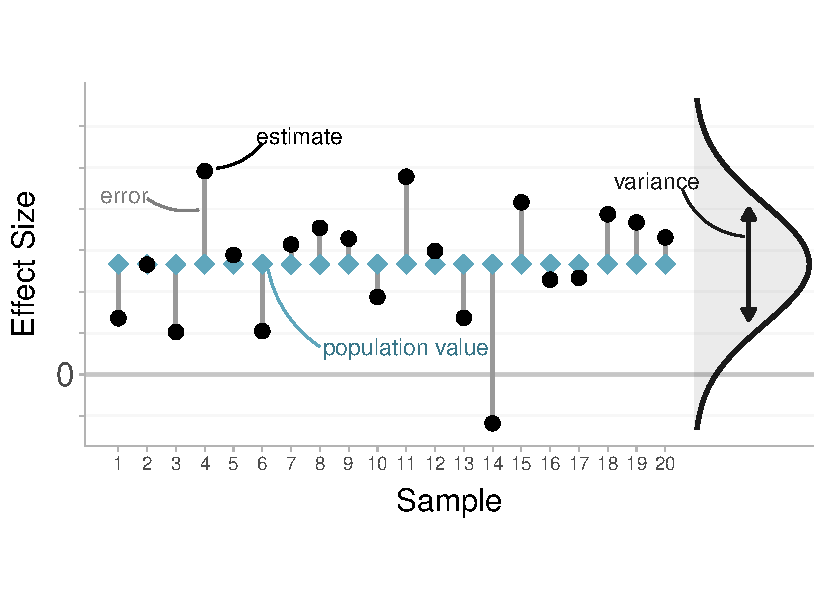
\includegraphics{chapters/01-definitions/01-definitions_files/figure-pdf/fig-3.1-1.pdf}

}

\caption{\label{fig-3.1}This figure shows the distribution of sample
estimates. The blue diamonds denotes the population effect size, which
stays constant across samples. The black dots denote the sample effect
size estimate. The grey lines denote random sampling errors, which
represent the difference between the estimates and the population value.
The sampling distribution on the right shows the probability
distribution of estimates across repeated samples, the width of this
distribution is described by the variance of the estimator. Note the
illustration shows a normally distributed estimator, but this is not a
requirement.}

\end{figure}%

\subsection{Systematic Errors}\label{systematic-errors}

Sampling errors produce random errors in effect sizes, however, we can
also observe systematic errors. \textbf{Systematic errors} are
deviations from the target population value that are consistent across
samples and produce bias in effect size estimates. In other words,
effect size estimates will be \emph{on average} larger or smaller than
the target population value (Barraza et al. 2019). Random sampling
errors, on the other hand, will be larger or smaller than the target
population value only by chance. \textbf{Attenuation} describes a type
of systematic error where the effect size estimates are \emph{smaller}
than the target population value on average. \textbf{Inflation} on the
other hand, is a type of bias that produce effect size estimates that
are \emph{larger} on average. An \textbf{unbiased} effect size would be
one where there is no systematic errors and therefore, on average, it is
equal to the population effect size. As we will see in future chapters,
study artifacts such as selection effects and measurement error can
produce effect sizes that contain systematic errors.

We can see in Figure~\ref{fig-systematic-errors} that the sampling
distribution does not become wider or smaller with systematic errors
(this may occur indirectly if the sampling variance depends on the
effect size itself), instead the whole sampling distribution shifts
downward or upward depending on whether the effect size estimates are
attenuated or inflated, respectively.

\begin{figure}[H]

\centering{

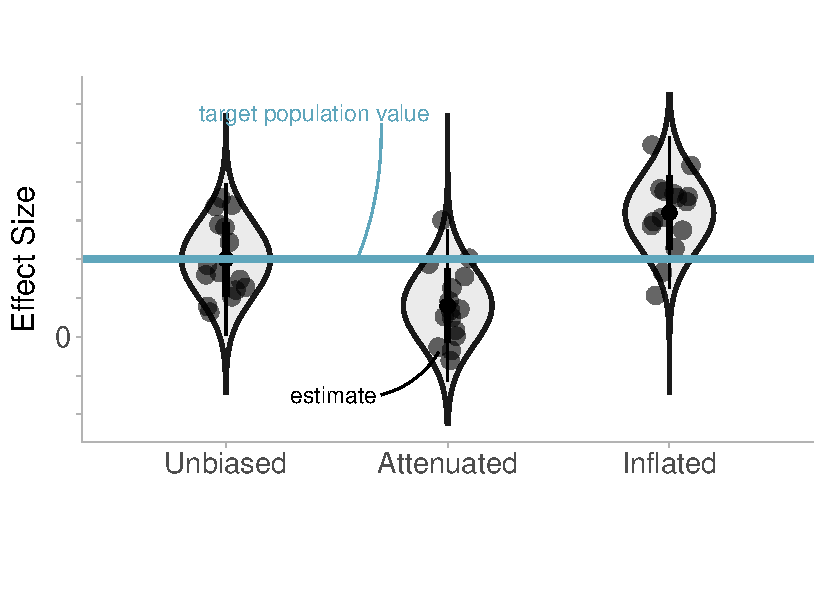
\includegraphics{chapters/01-definitions/01-definitions_files/figure-pdf/fig-systematic-errors-1.pdf}

}

\caption{\label{fig-systematic-errors}Three sampling distributions
representing estimators that are unbiased, attenuated, and inflated. The
blue line indicates the the location of the target population effect
size, whereas the black dots show the effect size estimates.}

\end{figure}%

\section{Modeling Observed Effect
Sizes}\label{modeling-observed-effect-sizes}

We can think of an observed effect size estimate as having three
components:

\includegraphics[width=5.56in,height=1.77in]{chapters/01-definitions/01-definitions_files/figure-latex/mermaid-figure-1.png}

Let's construct a statistical model for an observed effect size estimate
\(h_i\) for a given sample, \(i\), that accounts for each of these three
components. The \textbf{target population effect size}\} will be denoted
by the Greek letter \(\theta\) which does not vary from sample to
sample. The \textbf{artifact attenuation/inflation factor} is denoted
with the Greek letter \(\alpha\) and accounts for the systematic error
that is consistent across samples. Finally the \textbf{sampling error}
is denoted by the Greek letter \(\varepsilon\) which accounts for the
random sampling error across samples (Raju et al. 1991, based on eq. 1),

\begin{equation}\phantomsection\label{eq-model}{
h_i = \alpha \theta + \varepsilon_i.
}\end{equation}

Note that \(\alpha\) and \(\theta\) are fixed and does not vary across
samples (no subscript \(i\)), wheras \(\varepsilon_i\) does vary from
sample to sample. For the above equation to be true we need to assume
that the expectation (i.e., the mean over repeated samples) of
\(\varepsilon_i\) is zero such that, \(\mathbb{E}[\varepsilon_i] = 0\).
A consequence of this assumption is that the expectation of the observed
effect size estimate is \(\mathbb{E}[h_i]=\alpha \theta\). We will label
the term \(\alpha \theta\) as the \textbf{contaminated population effect
size} as it is a fixed value that encompasses the target effect size and
systematic error.

The artifact attenuation/inflation factor, \(\alpha\), completely
describes the net systematic error in the observed effect size
estimates. The value of \(\alpha\) can indicate whether \(h_i\) is an
unbiased (\(\alpha = 0\)), attenuated (\(\alpha < 1\)), or inflated
estimator (\(\alpha > 1\)).

Because of random sampling error, the observed effect size estimate will
differ from sample to sample (\(h_1\neq\) \(h_2\neq\) \(h_3\neq...\)).
The extent to which estimates fluctuate across samples can be quantified
by the variance of the effect size estimator, denoted as
\(\text{var}(h_i)\). Remember that the contaminated population effect
size (\(\alpha \theta\)) fixed across samples, this would result in
variation in random sampling errors to be solely responsible for the
variation in observed effect sizes such that,
\(\text{var}(h_i)=\text{var}(\varepsilon_i)\).

\section{Correcting Effect Sizes}\label{correcting-effect-sizes}

In principle, if we know the value of the artifact attenuation/inflation
factor \(\alpha\) then we could correct the observed effect size for
systematic errors. However, \(\alpha\) is unknown and must be estimated.
An estimate of \(\alpha\) will be denoted by the English letter \(a\).
According to the model described in Equation~\ref{eq-model}, \(\alpha\)
is a fixed value that does not vary from sample to sample, however it's
sample estimate will:

\begin{equation}\phantomsection\label{eq-a}{
a_i = \alpha + \xi_i,
}\end{equation}

where \(\xi_i\) denotes the sampling error in \(a_i\). The corrected
effect size can thus be calculated by dividing the observed effect size
by the estimated artifact factor,

\begin{equation}\phantomsection\label{eq-correction}{
h_{c_i} = \frac{h_i}{a_i},
}\end{equation}

The corrected effect size will only be an asymptotically (as the sample
size approaches infinity) unbiased estimator of the target population
value. As we will see in future chapters, corrections will also impose
additional distributional assumptions on the data.

Sampling variance of the corrected effect size will depend greatly on
the estimation procedure of the effect size and the artifact factor.
Sampling variance for corrected effect sizes will be discussed in more
detail for each artifact correction chapter.

\section{Effect Size Types}\label{effect-size-types}

Although there are many types of effect sizes we can use to quantify
research findings, we will primarily focus on two: correlations and
standardized mean differences (SMD).

\subsection{Correlations}\label{correlations}

A correlation describes the relationship between two continuous
variables. The population correlation (\(\rho\)) between variables,
\(X\) and \(Y\), can be defined as the covariance (\(\sigma_{XY}\))
divided by the product of the standard deviations of \(X\)
(\(\sigma_{X}\)) and \(Y\) (\(\sigma_{Y}\)) (Cooper, Hedges, and
Valentine 2009, equation 11.21; Jacobs and Viechtbauer 2017, eq. 1),

\begin{equation}\phantomsection\label{eq-pop-r}{
\rho = \frac{\sigma_{XY}}{\sigma_{X}\sigma_{Y}}.
}\end{equation}

A sample estimate of the population correlation can be defined as the
\emph{sample} covariance (\(S_{XY}\)) divided by the product of the
\emph{sample} standard deviations (Jacobs and Viechtbauer 2017, eq. 2),

\begin{equation}\phantomsection\label{eq-sam-r}{
r = \frac{S_{XY}}{S_XS_Y}
}\end{equation}

This is commonly referred to as the Pearson correlation coefficient. The
Pearson correlation coefficient was first introduced by Auguste Bravais
(1844), then later developed further by Karl Pearson, lending itself to
the name. See Figure~\ref{fig-r} for a visualization of correlated
variables.

\begin{figure}[H]

\centering{

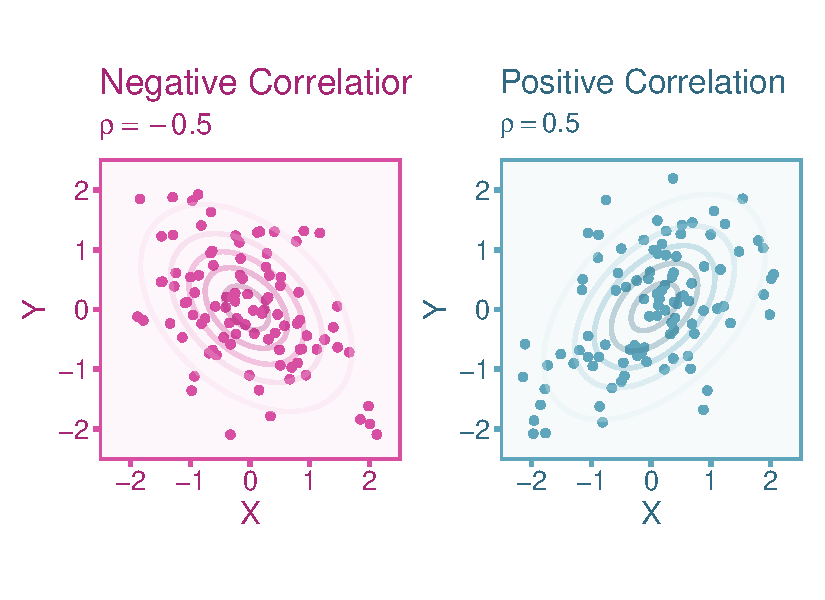
\includegraphics{chapters/01-definitions/01-definitions_files/figure-pdf/fig-r-1.pdf}

}

\caption{\label{fig-r}Diagram illustrating a correlation between two
variables (\(X\) and \(Y\)). The left panel shows a negative correlation
and the right panel shows a positive correlation. The ellipses show the
contour of a bivariate normal distribution which the data points are
sampled from.}

\end{figure}%

Assuming that the variables follow a bivariate normal distribution, the
asymptotic variance in an observed correlation with \(n\) observations
is (Pearson and Filon 1898, 174; Jacobs and Viechtbauer 2017, eq. 9),

\begin{equation}\phantomsection\label{eq-asymp-var-r}{
\text{var}(r_i) \overset{_\infty}{=} \frac{\left(1 - \rho^2\right)^2}{n},
}\end{equation}

Since the population correlation is unavailable in practice, an accurate
estimate of the variance for a given sample \(i\) uses the sample
correlation instead of population correlation and uses the degrees of
freedom, \(n-1\), in the denominator instead of the sample size (Cooper,
Hedges, and Valentine 2009, eq. 12.27; Jacobs and Viechtbauer 2017, eq.
10),

\begin{equation}\phantomsection\label{eq-est-var-r}{
\widehat{\text{var}}(r_i) = \frac{\left(1 - r_i^2\right)^2}{n-1}
}\end{equation}

Within the context of a research study that is contaminated with
artifacts, we can model an observed correlation for a sample \(i\) as
similarly to an Equation~\ref{eq-model},

\begin{equation}\phantomsection\label{eq-model-r}{
r_i = \alpha \rho + \varepsilon_i.
}\end{equation}

Where \(\rho\) is the target population correlation (the estimand),
\(\alpha\) is the artifact attenuation/inflation factor, and
\(\varepsilon_i\) denotes the sampling errors. The observed correlation
is biased relative to the target population correlation as a function of
\(\alpha\), and therefore a corrected correlation can calculated by,

\begin{equation}\phantomsection\label{eq-corr-r}{
r_{c_i} = \frac{r_i}{a_i}.
}\end{equation}

For example, we will see in Chapter~\ref{sec-dichotomization} that if
\(X\) and \(Y\) are bivariate normal and \(X\) undergoes dichotomization
through a median split (i.e., dividing observations into two groups
based on the median of \(X\)) the observed correlation will be
attenuated. In this scenario, the artifact attenuation/inflation factor
is \(a = 2/\sqrt{2\pi} \approx .80\), and therefore if the observed
correlation is \(r = .40\) then the corrected correlation would be
estimated as \(r_c=r/a=.40/.80=.50\).

\begin{tcolorbox}[enhanced jigsaw, opacityback=0, coltitle=black, toprule=.15mm, colframe=quarto-callout-note-color-frame, bottomtitle=1mm, rightrule=.15mm, colbacktitle=quarto-callout-note-color!10!white, left=2mm, bottomrule=.15mm, breakable, title={Computing Correlations in R}, colback=white, opacitybacktitle=0.6, titlerule=0mm, arc=.35mm, leftrule=.75mm, toptitle=1mm]

Let's load in the \texttt{iris} data set that contains various physical
measurements of three species of plants. We can also subset the data set
to only look at the Setosa species:

\begin{Shaded}
\begin{Highlighting}[]
\CommentTok{\# load in data}
\FunctionTok{data}\NormalTok{(}\StringTok{"iris"}\NormalTok{)}

\CommentTok{\# subset rows to only include setosa species}
\NormalTok{df }\OtherTok{\textless{}{-}} \FunctionTok{subset}\NormalTok{(iris, iris}\SpecialCharTok{$}\NormalTok{species }\SpecialCharTok{==} \StringTok{\textquotesingle{}setosa\textquotesingle{}}\NormalTok{)}

\CommentTok{\# view first 6 plants}
\FunctionTok{head}\NormalTok{(iris)}
\end{Highlighting}
\end{Shaded}

\begin{verbatim}
  Sepal.Length Sepal.Width Petal.Length Petal.Width Species
1          5.1         3.5          1.4         0.2  setosa
2          4.9         3.0          1.4         0.2  setosa
3          4.7         3.2          1.3         0.2  setosa
4          4.6         3.1          1.5         0.2  setosa
5          5.0         3.6          1.4         0.2  setosa
6          5.4         3.9          1.7         0.4  setosa
\end{verbatim}

Let's say we want to know the correlation between petal length and sepal
length. We can use the \texttt{cor()} function in base R to obtain the
Pearson correlation coefficient:

\begin{Shaded}
\begin{Highlighting}[]
\NormalTok{r }\OtherTok{\textless{}{-}} \FunctionTok{cor}\NormalTok{(iris}\SpecialCharTok{$}\NormalTok{Petal.Length,iris}\SpecialCharTok{$}\NormalTok{Sepal.Length)}
\NormalTok{r}
\end{Highlighting}
\end{Shaded}

\begin{verbatim}
[1] 0.8717538
\end{verbatim}

The result shows a strong positive correlation between petal and sepal
length (\(r = .87\)). To compute the sampling variance and the standard
error, we can use the \texttt{var\_error\_r()} function in the
\texttt{psychmeta} package (Dahlke and Wiernik 2019)

\begin{Shaded}
\begin{Highlighting}[]
\CommentTok{\# load in package}
\FunctionTok{library}\NormalTok{(psychmeta)}

\CommentTok{\# compute sampling variance}
\NormalTok{var\_r }\OtherTok{\textless{}{-}} \FunctionTok{var\_error\_r}\NormalTok{(r, }\AttributeTok{n =} \FunctionTok{nrow}\NormalTok{(iris), }\AttributeTok{correct\_bias =} \ConstantTok{FALSE}\NormalTok{)}

\CommentTok{\# print results}
\FunctionTok{data.frame}\NormalTok{(r,var\_r) }
\end{Highlighting}
\end{Shaded}

\begin{verbatim}
          r        var_r
1 0.8717538 0.0003867233
\end{verbatim}

\end{tcolorbox}

\subsection{Standardized Mean
Difference}\label{standardized-mean-difference}

The standardized mean differences (SMD) is used to quantify the
difference between the average value between two groups. In the
population, the SMD (\(\delta\)), the difference between the mean of
group \(A\) (\(\mu_A\)) and group \(B\) (\(\mu_B\)) is standardized by
the population within group standard deviation (\(\sigma\)) (Cohen 1988,
eq. 2.2.1),

\begin{equation}\phantomsection\label{eq-delta}{
\delta = \frac{\mu_A - \mu_B}{\sigma}.
}\end{equation}

Dividing by the population within-group standard deviation assumes that
the standard deviations within both groups are fixed and equal (i.e.,
\(\sigma=\sigma_A=\sigma_B\)). For a visualization of an SMD see
Figure~\ref{fig-d}.

\begin{figure}[H]

\centering{

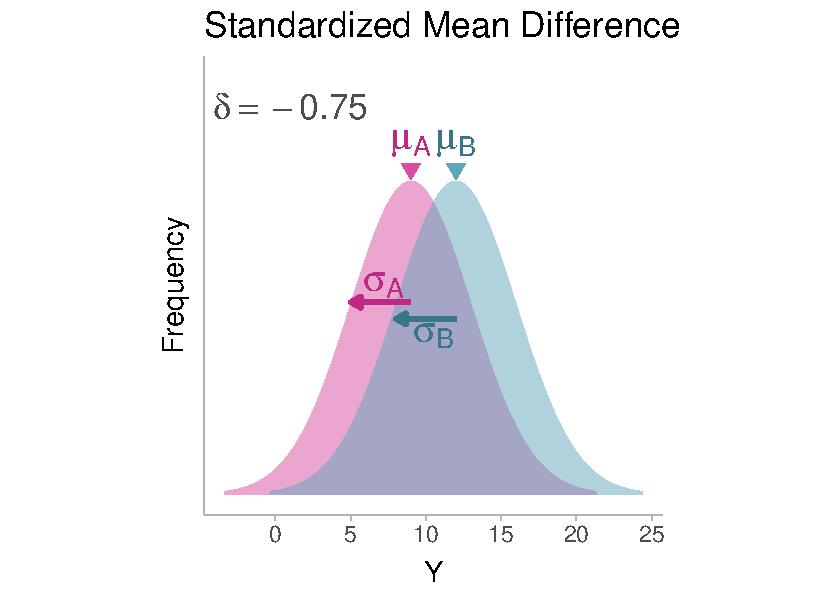
\includegraphics{chapters/01-definitions/01-definitions_files/figure-pdf/fig-d-1.pdf}

}

\caption{\label{fig-d}Diagram illustrating a standardized mean
difference in the population between two normal distributions. The mean
and standard deviation of group \(A\) is \(\mu_A=9\) and \(\sigma_A=4\),
respectively. Whereas mean and standard deviation of group \(B\) is
\(\mu_A=12\) and \(\sigma_A=4\), respectively. Therefore the
standardized mean difference is \(\delta = (9-12)/4=-.75\). Note that
\(\sigma_A=\sigma_B\).}

\end{figure}%

Cohen (1988) developed a sample estimator of \(\delta\) that is commonly
referred to as Cohen's \(d\). Within a sample, we can estimate
\(\delta\) with the sample estimator (Cooper, Hedges, and Valentine
2009, eq. 11.96),

\begin{equation}\phantomsection\label{eq-d}{
d = \frac{\overline{Y}_A-\overline{Y}_B}{S_p},
}\end{equation}

where \(S_p\) is the pooled sample standard deviation and the bars
indicate the sample mean. The pooled standard deviation computes a
weighted average (weighted by the within-group degrees of freedom, e.g.,
\(n_{A}-1\)) of the within-group sample variance and then takes the
square root (Cooper, Hedges, and Valentine 2009, eq. 12.12),

\begin{equation}\phantomsection\label{eq-pooled-sd}{
S_p = \sqrt{\frac{(n_A-1)S_A^2 + (n_B-1)S_B^2}{n-2}}
}\end{equation}

Where \(n_A\), \(n_B\), and \(n\) represent the sample size within group
\(A\), group \(B\), and the total sample size (\(n = n_A+n_B\)),
respectively. Assuming that \(Y\) is normally distributed within each
group and the within-group variances are equal, the asymptotic sampling
variance of an SMD is (Hedges and Olkin 1985, eq. 14),

\begin{equation}\phantomsection\label{eq-var-d}{
\text{var}(d_i) \overset{_\infty}{=} \frac{n}{n_An_B} + \frac{\delta^2}{2n}.
}\end{equation}

Since the population SMD is unknown, we can estimate it with the sample
\(d\) value. Therefore the estimated variance can be computed as (J. E.
Hunter and Schmidt 2015, eq. 7.23),

\begin{equation}\phantomsection\label{eq-var-d-est}{
\widehat{\text{var}}(d_i) = \left(\frac{n - 1}{n - 3}\right)\left(\frac{n}{n_An_B} + \frac{\delta^2}{2n}\right).
}\end{equation}

Note that the multiplier, \((n_A+n_B - 1)/(n_A+n_B - 3)\), is to account
for slight underestimation of the sampling variance in small sample
sizes (Goulet-Pelletier and Cousineau 2018).

In a study contaminated by artifacts, we can model an observed SMD for a
sample \(i\) as similarly to an Equation~\ref{eq-model},

\begin{equation}\phantomsection\label{eq-model-d}{
d_i =\alpha \delta + 
\varepsilon_i.
}\end{equation}

Where \(\delta\) is the {target population SMD (the estimand)},
\(\alpha\) is the {artifact attenuation/inflation factor}, and
\(\varepsilon_i\) denotes the {sampling errors}. The observed SMD is
biased relative to the target population SMD as a function of
\(\alpha\). However, \(\alpha\) is not available in practice and so
therefore the observed SMD can be corrected by dividing by an estimate
of \(\alpha\),

\begin{equation}\phantomsection\label{eq-corr-d}{
d_{c_i} = \frac{d_i}{a_i}.
}\end{equation}

Occasionally, corrections can not be applied to the contaminated \(d\)
value directly. In such cases, we may have to correct \(d\) by first
converting to a \emph{point-biserial} correlation (i.e., a Pearson
correlation between a dichotomous group variable and continuous
variable), correcting the correlation, and then converting back to a
(corrected) \(d\) value (J. E. Hunter and Schmidt 2015). The three-step
procedure can be applied as follows:

\begin{enumerate}
\def\labelenumi{\arabic{enumi}.}
\tightlist
\item
  Convert \(d\) to \(r\) using the proportion of subjects in group \(A\)
  or group \(B\) (\(p=n_A/n\) or \(p=n_B/n\)) (Wiernik and Dahlke 2020,
  equation 9),
\end{enumerate}

\begin{equation}\phantomsection\label{eq-three-step-1}{
r_i = \frac{d_i}{\sqrt{\frac{1}{p_i(1-p_i)}+d_i}}.
}\end{equation}

\begin{enumerate}
\def\labelenumi{\arabic{enumi}.}
\setcounter{enumi}{1}
\tightlist
\item
  Correct the point-biserial correlation,
\end{enumerate}

\[
{\color{#347e9f}r_c}_{_i} = \frac{r_i}{a_i}.
\]

\begin{enumerate}
\def\labelenumi{\arabic{enumi}.}
\setcounter{enumi}{2}
\tightlist
\item
  Convert \(r_c\) back to a \(d\) value. If the proportions of group
  membership are contaminated by artifacts, then we need the true group
  proportions in the target population (\(p_i^*\)) to convert back to
  \(d\). If the the true group proportions are unavailable, then we can
  use the observed proportions as estimates (Wiernik and Dahlke 2020,
  equation 10)
\end{enumerate}

\begin{equation}\phantomsection\label{eq-three-step-3}{
d_{c_i} =  \frac{r_{c_i}}{\sqrt{p_i^*(1-p_i^*)(1-r_{c_i}^2)}} \approx \frac{r_{c_i}}{\sqrt{p_i(1-p_i)(1-r_{c_i}^2)}}.
}\end{equation}

The sampling variance of the corrected SMD can be quite complicated when
there is sampling error in the artifact factor.

\begin{tcolorbox}[enhanced jigsaw, opacityback=0, coltitle=black, toprule=.15mm, colframe=quarto-callout-note-color-frame, bottomtitle=1mm, rightrule=.15mm, colbacktitle=quarto-callout-note-color!10!white, left=2mm, bottomrule=.15mm, breakable, title={Computing SMDs in R}, colback=white, opacitybacktitle=0.6, titlerule=0mm, arc=.35mm, leftrule=.75mm, toptitle=1mm]

Let's load in a data set for a plant growth experiment:

\begin{Shaded}
\begin{Highlighting}[]
\CommentTok{\# load in data}
\FunctionTok{data}\NormalTok{(}\StringTok{"PlantGrowth"}\NormalTok{)}

\CommentTok{\# view first 6 plants}
\FunctionTok{head}\NormalTok{(PlantGrowth)}
\end{Highlighting}
\end{Shaded}

\begin{verbatim}
  weight group
1   4.17  ctrl
2   5.58  ctrl
3   5.18  ctrl
4   6.11  ctrl
5   4.50  ctrl
6   4.61  ctrl
\end{verbatim}

We see that the data set contains two variables, weight of the plant and
the experimental group. There are three two experimental groups present:
a control group and two treatment groups. If we want to obtain the SMD
between the each treatment group and the control group, we can use the
\texttt{cohen.d} function \texttt{psych} package (William Revelle 2023):

\begin{Shaded}
\begin{Highlighting}[]
\FunctionTok{library}\NormalTok{(psych)}

\CommentTok{\# estimate SMD for first treatment group}
\NormalTok{d1 }\OtherTok{\textless{}{-}} \FunctionTok{cohen.d}\NormalTok{(weight }\SpecialCharTok{\textasciitilde{}}\NormalTok{ group,}
             \AttributeTok{data =} \FunctionTok{subset}\NormalTok{(PlantGrowth, group }\SpecialCharTok{==} \StringTok{\textquotesingle{}ctrl\textquotesingle{}} \SpecialCharTok{|}\NormalTok{ group }\SpecialCharTok{==} \StringTok{\textquotesingle{}trt1\textquotesingle{}}\NormalTok{))}
\NormalTok{d1}\SpecialCharTok{$}\NormalTok{cohen.d}
\end{Highlighting}
\end{Shaded}

\begin{verbatim}
          lower     effect     upper
weight -1.44938 -0.5615655 0.3411078
\end{verbatim}

\begin{Shaded}
\begin{Highlighting}[]
\CommentTok{\# estimate SMD for first treatment group}
\NormalTok{d2 }\OtherTok{\textless{}{-}} \FunctionTok{cohen.d}\NormalTok{(weight }\SpecialCharTok{\textasciitilde{}}\NormalTok{ group,}
              \AttributeTok{data =} \FunctionTok{subset}\NormalTok{(PlantGrowth, group }\SpecialCharTok{==} \StringTok{\textquotesingle{}ctrl\textquotesingle{}} \SpecialCharTok{|}\NormalTok{ group }\SpecialCharTok{==} \StringTok{\textquotesingle{}trt2\textquotesingle{}}\NormalTok{))}
\NormalTok{d2}\SpecialCharTok{$}\NormalTok{cohen.d}
\end{Highlighting}
\end{Shaded}

\begin{verbatim}
            lower   effect    upper
weight 0.05850126 1.005987 1.929048
\end{verbatim}

We see that the first treatment showed a negative effect on plant growth
(\(d=-0.56\)) and the second treatment shows a positive effect
(\(d=1.01\)). For our purposes we want the estimate and the sampling
variance of the estimator, therefore we can extract that information
from the output of \texttt{cohen.d()}:

\begin{Shaded}
\begin{Highlighting}[]
\FunctionTok{data.frame}\NormalTok{(}\AttributeTok{d =}\NormalTok{ d1}\SpecialCharTok{$}\NormalTok{cohen.d[,}\StringTok{\textquotesingle{}effect\textquotesingle{}}\NormalTok{], }
           \AttributeTok{var.d =}\NormalTok{ d1}\SpecialCharTok{$}\NormalTok{se}\SpecialCharTok{\^{}}\DecValTok{2}\NormalTok{)}
\end{Highlighting}
\end{Shaded}

\begin{verbatim}
           d     var.d
1 -0.5615655 0.8014621
\end{verbatim}

\begin{Shaded}
\begin{Highlighting}[]
\FunctionTok{data.frame}\NormalTok{(}\AttributeTok{d =}\NormalTok{ d2}\SpecialCharTok{$}\NormalTok{cohen.d[,}\StringTok{\textquotesingle{}effect\textquotesingle{}}\NormalTok{], }
           \AttributeTok{var.d =}\NormalTok{ d2}\SpecialCharTok{$}\NormalTok{se}\SpecialCharTok{\^{}}\DecValTok{2}\NormalTok{)}
\end{Highlighting}
\end{Shaded}

\begin{verbatim}
         d     var.d
1 1.005987 0.8747367
\end{verbatim}

\end{tcolorbox}

\bookmarksetup{startatroot}

\chapter{Small Samples}\label{small-samples}

\section{Introduction}\label{introduction-1}

The purpose of sample statistics is to draw meaningful inferences about
the population. However, effect size estimators such as Pearson's
correlation coefficient and Cohen's \(d\) are biased in small sample
sizes. This small sample bias is an artifact and can be adjusted with
the appropriate correction factor.

\section{When Correcting alongside other
Artifacts}\label{when-correcting-alongside-other-artifacts}

The small sample bias should always be corrected for prior to applying
any other artifact correction. It is independent of all other artifact
corrections and therefore the corrected effect sizes in this section can
be treated as the uncorrected effect sizes in other sections.

\section{Correcting Standardized Mean Differences for Small Sample
Bias}\label{correcting-standardized-mean-differences-for-small-sample-bias}

\subsection{Defining the Target
Quantity}\label{defining-the-target-quantity}

Our quantity of interest is the population standardized mean difference,
\(\delta\), between groups \(A\) and \(B\). We can model the
relationship between the population standardized mean difference and the
estimate (\(d\)),

\[
d = a\delta+e.
\]

Where \(a\) is an attenuation/inflation factor and \(e\) is our sampling
error term. Ultimately, we can obtain an unbiased estimate of the
population standardized mean difference by correcting the sample
standardized mean difference as follows,

\[
d_c = \frac{d}{\hat{a}}.
\]

\subsection{\texorpdfstring{Artifact Correction for
\emph{d}}{Artifact Correction for d}}\label{artifact-correction-for-d}

As the sample size approaches infinity, Cohen's estimator of the
standardized mean difference is unbiased (Hedges 1981; Cohen 2013).
However, in small sample sizes Cohen's estimator is inflated, that is,
on average, it overestimates the population standardized mean
difference. To see why this is the case, we can first define the
population standardized mean difference between group \(A\) and group
\(B\) such that,

\[
\delta = \frac{\mu_A-\mu_B}{\sigma}.
\]

Where \(\bar{y}_A\) and \(\bar{y}_B\) are the observed arithmetic means
of group \(A\) and group \(B\), respectively. A sample estimate of the
standardized mean difference is,

\begin{equation}\phantomsection\label{eq-d}{
d = \frac{\overline{Y}_A-\overline{Y}_B}{S_p}
}\end{equation}

Where \(S_p\) is the pooled standard deviation (i.e., weighted average
within-group standard deviation). The estimator, \(d\), is an
asymptotically unbiased estimate of \(\delta\). We can denote this
asymptotic relationship as,

\[
\mathbb{E}_i[d_i] \overset{_n}{\asymp} \delta.
\]

However, \(d\) is a biased estimator of \(\delta\) when the sample size
is finite. Particularly, the smaller the sample size, the larger the
bias. We can see that in Figure~\ref{fig-d-bias}, \(d\) tends to
over-estimate \(\delta\). Therefore, we can apply an artifact inflation
factor, \(a\), to capture this over-estimation,

\[
\mathbb{E}_i[d_i] = a\delta.
\]

The reason for this bias in \(d\) values is two-fold:

\begin{itemize}
\tightlist
\item
  Standard deviations tend to be attenuated in small sample sizes. This
  is due to the fact that although variance (squared standard deviation)
  is an unbiased estimator of the population variance, the square root
  of the variance (i.e., the standard deviation, \(S_p\)) is a biased
  estimate of the population standard deviation
  (\(\mathbb{E}_i[\sqrt{S_{p_i}}] \neq \sqrt{\sigma}\), Holtzman 1950).
\item
  A ratio is biased in small sample sizes (Kempen and Vliet 2000),
  therefore the ratio between the mean difference and the standard
  deviation (see Equation~\ref{eq-d}) will likewise be biased.
\end{itemize}

To obtain an unbiased estimate of the population standardized mean
difference, we need to first estimate the artifact inflation factor,
\(a\). In this case, the artifact inflation factor has been
mathematically derived previously by Hedges (1989). For other types of
artifacts, \(a\) is unknown in practice and must be estimated, however,
for small sample bias the exact value of \(a\) is known. The precise
value of \(a\) is a function of sample size (equation 6e, Hedges 1989),

\[
a = \frac{\Gamma\left(\frac{n-3}{2}\right)\sqrt{\frac{n-2}{2}}}{\Gamma\left(\frac{n-2}{2}\right)}.
\] Where \(\Gamma(\cdot)\) denotes the gamma function. The gamma
function is factorial function generalized to non-integers (note that a
factorial function on integers would look something like:
\(3! = 3 \cdot 2 \cdot 1\), Taboga 2021). There is also an approximation
of \(a\) that is more computationally trivial (re-arrangement of the
first formula on pp.~114, Hedges 1989):

\[
a \approx \frac{4n-9}{4n-12}
\]

However, with the advent of computers, this approximation formula is
unnecessary. We can see in Figure~\ref{fig-r-bias} that there is notable
bias when sample size is below 20. Furthermore, the bias is most
pronounced when the sample \(d\) value is larger (there is no bias at
\(d=0\)).

\begin{figure}[H]

\centering{

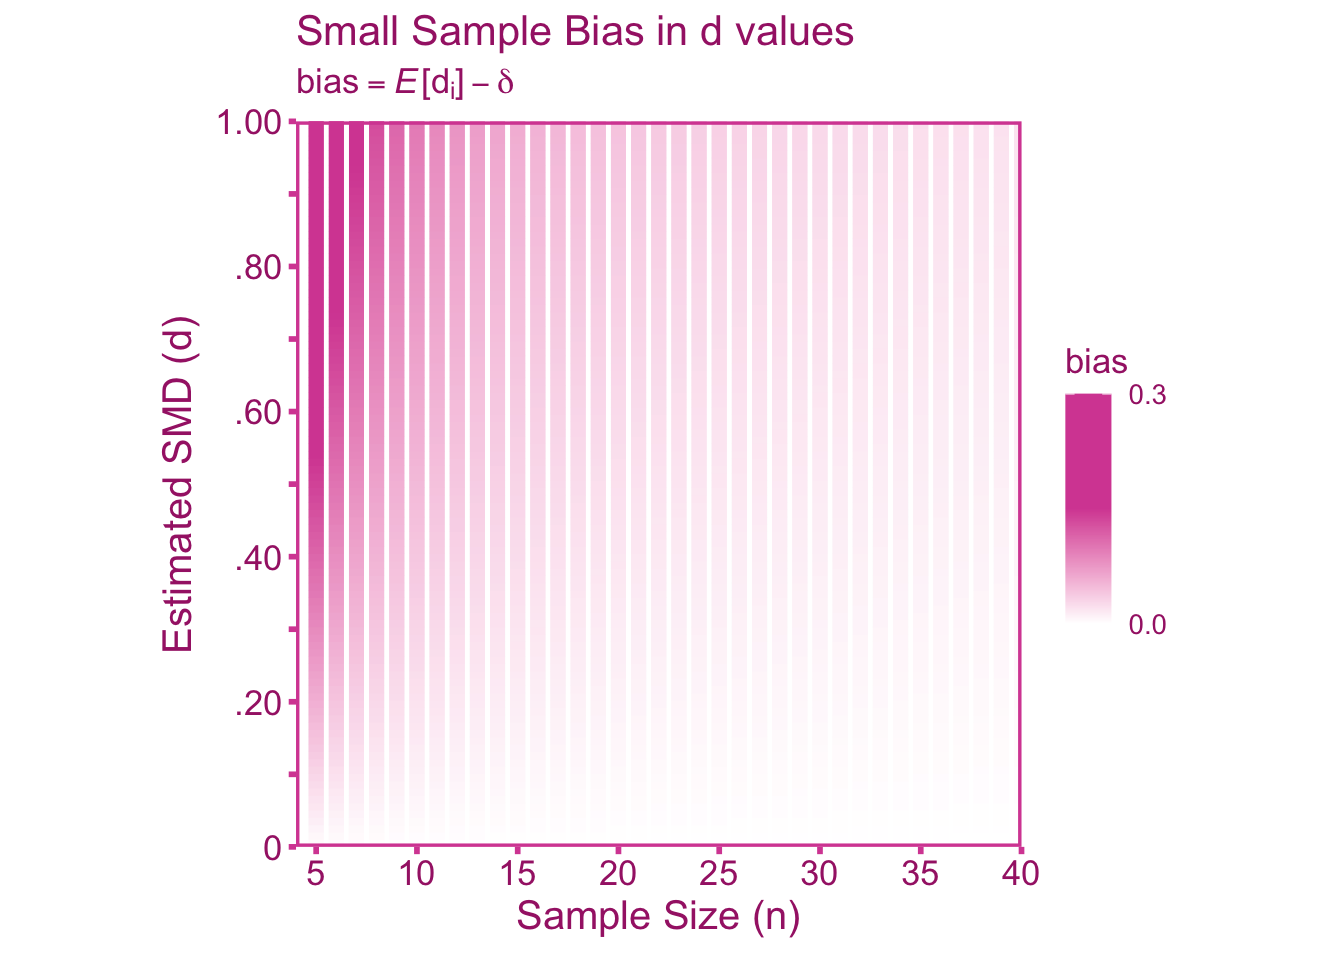
\includegraphics{chapters/02-small-samples/02-small-samples_files/figure-pdf/fig-d-bias-1.pdf}

}

\caption{\label{fig-d-bias}Plot showing the bias in the standardized
mean difference computed in small samples. The X-axis is the sample size
(\(n\), the vertical bars are indicative of each integer). The Y-axis is
the the estimated standardized mean difference (\(d\)). The dark pink
coloring indicates more bias.}

\end{figure}%

Using \(a\), we can correct the \(d\) value such that,

\begin{equation}\phantomsection\label{eq-d-corr}{
d_c = \frac{d}{a} = \frac{d}{ \left[\frac{\Gamma\left(\frac{n-3}{2}\right)\sqrt{\frac{n-2}{2}}}{\Gamma\left(\frac{n-2}{2}\right)}\right]}.
}\end{equation}

To obtain the standard error of \(d_c\) we can apply the same correction
as above to the standard error of \(d\) (\(se\)),

\begin{equation}\phantomsection\label{eq-se-corr-d}{
se(d_c) = \frac{se(d)}{a} = \frac{se(d)}{ \left[\frac{\Gamma\left(\frac{n-3}{2}\right)\sqrt{\frac{n-2}{2}}}{\Gamma\left(\frac{n-2}{2}\right)}\right]}.
}\end{equation}

\begin{tcolorbox}[enhanced jigsaw, opacityback=0, coltitle=black, toprule=.15mm, colframe=quarto-callout-note-color-frame, bottomtitle=1mm, rightrule=.15mm, colbacktitle=quarto-callout-note-color!10!white, left=2mm, bottomrule=.15mm, breakable, title={Applied Example in R}, colback=white, opacitybacktitle=0.6, titlerule=0mm, arc=.35mm, leftrule=.75mm, toptitle=1mm]

Let's say we want to compute the mean difference of test scores between
two classes. Class 1 has 11 students and class 2 has 10 students. We
then obtain a standardized mean difference between the two classes of
\(d=.43\). In R, we can use the \texttt{correct\_d\_bias()} function to
correct the point estimate (using Equation~\ref{eq-d-corr}) and then
\texttt{var\_error\_g} function to correct the error variance and thus
the standard error (using Equation~\ref{eq-se-corr-d}). Both of these
functions are found in the \texttt{psychmeta} package (Dahlke and
Wiernik 2019).

\begin{Shaded}
\begin{Highlighting}[]
\FunctionTok{library}\NormalTok{(psychmeta)}

\NormalTok{d }\OtherTok{\textless{}{-}}\NormalTok{ .}\DecValTok{43}
\NormalTok{n1 }\OtherTok{\textless{}{-}} \DecValTok{11}
\NormalTok{n2 }\OtherTok{\textless{}{-}} \DecValTok{10}

\CommentTok{\# correct}
\NormalTok{dc }\OtherTok{\textless{}{-}} \FunctionTok{correct\_d\_bias}\NormalTok{(}\AttributeTok{d =}\NormalTok{ d,}
                     \AttributeTok{n =}\NormalTok{ n1}\SpecialCharTok{+}\NormalTok{n2)}

\NormalTok{var\_corrected }\OtherTok{\textless{}{-}} \FunctionTok{var\_error\_g}\NormalTok{(}\AttributeTok{g =}\NormalTok{ dc, }
                             \AttributeTok{n1 =}\NormalTok{ n1, }
                             \AttributeTok{n2 =}\NormalTok{ n2)}

\CommentTok{\# print results}
\FunctionTok{cbind}\NormalTok{(}\AttributeTok{dc=}\NormalTok{dc, }\AttributeTok{se =} \FunctionTok{sqrt}\NormalTok{(var\_corrected))}
\end{Highlighting}
\end{Shaded}

\begin{verbatim}
            dc       se
[1,] 0.4144264 0.424262
\end{verbatim}

The output shows a corrected standardized mean difference of
\(d_c = 0.41\) (\(se(d_c) = 0.42\))

\end{tcolorbox}

\section{Correcting for Small Sample Bias in
Correlations}\label{correcting-for-small-sample-bias-in-correlations}

\subsection{Defining the Estimand}\label{defining-the-estimand}

Our quantity of interest is the population correlation, \(\rho\). We can
model the relationship between the population correlation and our sample
estimate (\(r\)) with,

\[
r = a\rho+e
\]

Where \(a\) is our small sample biasing factor and \(e\) is our sampling
error term. Ultimately, we can obtain an unbiased estimate of the
population correlation by correcting the observed correlation as
follows,

\[
r_c = \frac{r}{a}
\]

\subsection{\texorpdfstring{Artifact Correction for
\emph{r}}{Artifact Correction for r}}\label{artifact-correction-for-r}

Let's first define the correlation in the population as the covariance
between \(X\) and \(Y\) (\(\sigma_{XY}\)) standardized by the product of
the standard deviation of \(X\) (\(\sigma_X\)) and \(Y\) (\(\sigma_Y\)):

\[
\rho = \frac{\sigma_{XY}}{\sigma_{X}\sigma_Y}
\]

The sample estimate can be defined as (\(S\) denoting the sample
estimates of \(\sigma\)),

\[
r = \frac{S_{XY}}{S_{X}S_Y}
\]

Asymptotically, the expectation of a sample correlation is equal to the
population correlation,

\[
\mathbb{E}_i[r_i] \overset{_n}{\asymp} \rho.
\]

However, similar to standardized mean differences, correlations are also
biased in small sample sizes (Olkin and Pratt 1958). Unlike standardized
mean differences, Pearson correlations are \emph{under}-estimated,
rather than over-estimated. Therefore, an artifact \emph{attenuation}
factor, \(a\), can account for this bias,

\[
\mathbb{E}_i[r_i] = a\rho.
\]

Because the attenuation factor, \(a\), has been mathematically derived
directly Olkin and Pratt (equation 2.3, 1958), there is no need to
obtain a noisy estimate of \(a\). Therefore \(a\) can be defined exactly
as,

\begin{equation}\phantomsection\label{eq-a-r}{
a = \frac{1}{F\left(\frac{1}{2},\frac{1}{2};\frac{n-1}{2};1-r^2\right)}
}\end{equation}

Where \(F(\cdot)\) is the hypergeometric function (for background see
the Wikipedia page: ). The hypergeometric function is a complicated and
iterative function which which can be defined in terms of
\(\Gamma(\cdot)\) functions (plugging in values into equation 2.2, Olkin
and Pratt 1958)

\[
F\left(\frac{1}{2},\frac{1}{2};\frac{n-1}{2};1-r^2\right) = \sum^{\infty}_{z=0} \frac{\Gamma\left(\frac{1}{2} + z\right)\Gamma\left(\frac{n-1}{2}\right)\left(1-r^2\right)^z}{\Gamma\left(\frac{1}{2}\right)\Gamma\left(\frac{n-1}{2}+z\right)z!}
\]

Although this formula is complex, it can be easily done in R so do not
worry! There is also an approximation of \(a\) that is much simpler than
Equation~\ref{eq-a-r},

\[
a \approx \frac{2(n-3)}{2n-r^2-5}
\]

Then we can correct the point-estimate the sampling variance for small
sample bias. I will emphasize that approximations are not necessary if a
computer is available. We can see in Figure~\ref{fig-r-bias} that there
is notable bias when sample size is below 15. Furthermore, the bias is
most pronounced when the sample correlation around .60 (there is no bias
at \(r=0\) and \(r=\pm 1\)).

\begin{figure}[H]

\centering{

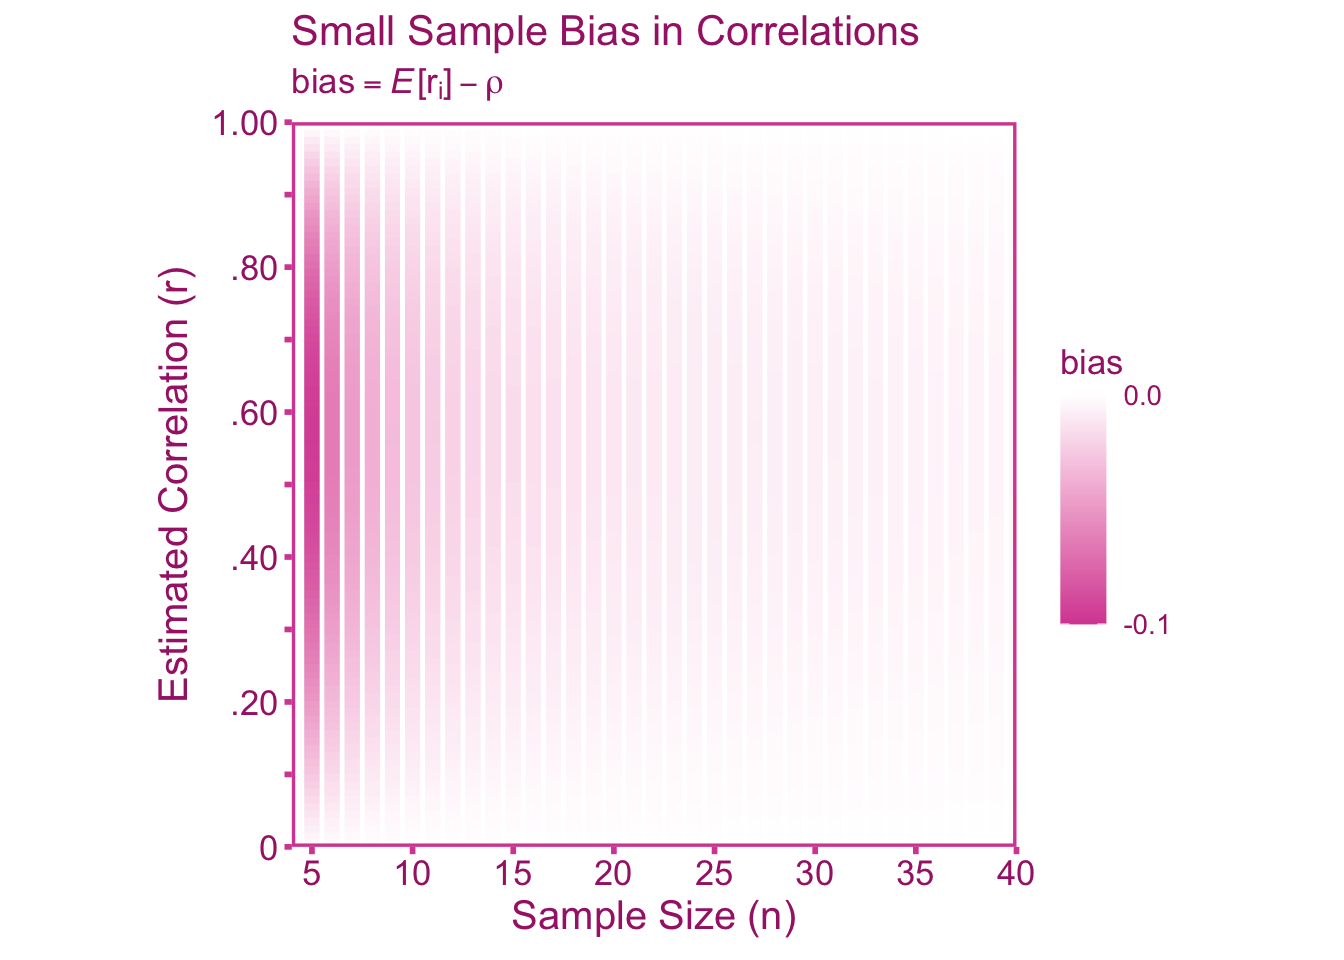
\includegraphics{chapters/02-small-samples/02-small-samples_files/figure-pdf/fig-r-bias-1.pdf}

}

\caption{\label{fig-r-bias}Plot showing the bias in the correlations
computed in small samples. The X-axis is the sample size (\(n\), the
vertical bars are indicative of each integer). The Y-axis is the the
estimated Pearson correlation (\(r\)). The dark pink coloring indicates
more bias.}

\end{figure}%

To correct for small sample bias, we can divide the sample correlation
\(r\) by the attenuation factor \(a\),

\begin{equation}\phantomsection\label{eq-r-corr}{
r_c = \frac{r}{a} = \frac{r}{\left[\frac{1}{F\left(\frac{1}{2},\frac{1}{2};\frac{n-1}{2};1-r^2\right)}\right]}
}\end{equation}

Where the standard error of \(r_c\) can be obtained by correcting the
observed standard error (\(se\)),

\begin{equation}\phantomsection\label{eq-se-corr}{
se(r_c) = \frac{se(r)}{a} = \frac{se(r)}{\left[\frac{1}{F\left(\frac{1}{2},\frac{1}{2};\frac{n-1}{2};1-r^2\right)}\right]}
}\end{equation}

\begin{tcolorbox}[enhanced jigsaw, opacityback=0, coltitle=black, toprule=.15mm, colframe=quarto-callout-note-color-frame, bottomtitle=1mm, rightrule=.15mm, colbacktitle=quarto-callout-note-color!10!white, left=2mm, bottomrule=.15mm, breakable, title={Applied Example in R}, colback=white, opacitybacktitle=0.6, titlerule=0mm, arc=.35mm, leftrule=.75mm, toptitle=1mm]

Let's say we compute a correlation of \(r=.43\) between test scores and
self-reported motivation in a small sample of students. In R, we can use
the \texttt{escalc} function in the \texttt{metafor} package
(Viechtbauer 2010). Setting \texttt{measure\ =\ "UCOR"} will apply the
small sample correction for the point estimate
(Equation~\ref{eq-r-corr}) and the error variance (i.e., square of the
standard error, Equation~\ref{eq-se-corr}). Note in order to run this
function you must have the \texttt{gsl} package already installed.

\begin{Shaded}
\begin{Highlighting}[]
\CommentTok{\# install.packages(\textquotesingle{}gsl\textquotesingle{})}
\FunctionTok{library}\NormalTok{(metafor)}

\NormalTok{r }\OtherTok{\textless{}{-}}\NormalTok{ .}\DecValTok{43}
\NormalTok{n }\OtherTok{\textless{}{-}} \DecValTok{11}

\CommentTok{\# correct the correlation}
\FunctionTok{escalc}\NormalTok{(}\AttributeTok{measure =} \StringTok{\textquotesingle{}UCOR\textquotesingle{}}\NormalTok{,}
       \AttributeTok{ri =}\NormalTok{ r,}
       \AttributeTok{ni =}\NormalTok{ n,}
       \AttributeTok{var.names =} \FunctionTok{c}\NormalTok{(}\StringTok{"rc"}\NormalTok{, }\StringTok{"se.2"}\NormalTok{),}
       \AttributeTok{digits =} \DecValTok{3}\NormalTok{)}
\end{Highlighting}
\end{Shaded}

\begin{verbatim}

     rc  se.2 
1 0.454 0.063 
\end{verbatim}

The output shows a corrected correlation between test scores and
motivation of \(r_c=.454\) (\(se(r)^2=.063\)).

\end{tcolorbox}

\bookmarksetup{startatroot}

\chapter{Introduction to Measurement
Error}\label{introduction-to-measurement-error}

\bookmarksetup{startatroot}

\chapter{Unreliability}\label{unreliability}

\section{Introduction}\label{introduction-2}

In general terms, measurement is the process of quantifying an attribute
or characteristic of something. In scientific measurement, the measurand
is the quantity or the attribute we intend to measure. In the
psychological sciences, measurands usually take the form of constructs
such as intelligence or anxiety. Often the goal of measurement is to
produce quantities (i.e., scores) that accurately reflect the measurand.
However, quantities that do not reflect a \emph{real} attribute can
still have useful predictive value (e.g., socio-economic status). It is
important to note that measures are not all created equal, some perform
better than others. Ideally, measures should produce scores that are
consistent and repeatable, this is referred to as the \emph{reliability}
of a measure. A high quality measure should produce highly reliable
scores. This section will review what reliability is in theory, how to
estimate reliability, and how to correct effect sizes for measurement
error.

\section{Reliability in True Score Theory}\label{sec-true-score-theory}

True score theory (or classical test theory) is a mathematical
formalization of observed scores obtained from a measurement procedure.
Observed scores, \(X_m\), is defined as a score obtained upon
measurement \(m\). The true score model assumes that each individual,
has a true score, \(T\), that stays constant over repeated measurements.
Variation in observed scores over repeated measurements is due to
measurement-specific error, \(E_{m}\),

\[
X_{m} = T+E_{m}.
\]

Here, measurements are \emph{strictly parallel}. Strictly parallel
measurements have the following four properties (p.~69, Haertel 2006):

\begin{enumerate}
\def\labelenumi{\arabic{enumi}.}
\tightlist
\item
  Measurements have identical specifications. That is, each measurement
  uses the same measurement procedure.
\item
  The distribution of observed scores for each measurement are
  identical: \(f(X_1) = f(X_2) = \ldots\).
\item
  Any set of two measurements are assumed to covary the same as any
  other set of two measurements:
  \(\sigma_{X_1 X_2} = \sigma_{X_2 X_3} = \sigma_{X_1 X_3} = \ldots\).
\item
  Each measurement equally covaries with any other variable:
  \(\sigma_{X_1 Y} = \sigma_{X_2 Y} = \ldots\).
\end{enumerate}

True scores can be defined as the expected value (i.e., the mean) of
observed scores over repeated measurements such that,
\(\mathbb{E}_m[X_{m}]=T\). Given this assumption, it follows that the
average of the resultant errors is zero across repeated measurements,
\(\mathbb{E}_m[E_{m}]=0\). It also follows that the covariance between
observed scores from measurement to measurement must only be
attributable to the variation in true scores
(\(\sigma_{XX'}=\sigma^2_{T}\)) and therefore true scores and errors are
independent (\(\sigma_{ET}=0\)). The independence between true scores
and errors provide convenient parsing of the variance in observed
scores,

\begin{equation}\phantomsection\label{eq-variance}{
\sigma_{X}^2 = \sigma_T^2 + \sigma_{E}^2.
}\end{equation}

In practice, the goal is to obtain observed scores that closely resemble
true scores, therefore it is important to minimize measurement error
variance (\(\sigma^2_E\)). If \(\sigma^2_E = 0\), then the scores can be
said to have perfect reliability, that is, observed scores do not vary
upon repeated measurements and are thus identical to true scores. In
practice, this is virtually never the case. In true score theory,
\emph{reliability} can be defined as the correlation between observed
scores in parallel measurements,

\[
\rho_{XX'}=\frac{\sigma_{XX'}}{\sigma_X\sigma_{X'}}  = \frac{\sigma_T^2}{\sigma^2_X}.
\]

The reliability can also be expressed by the square of the correlation
between observed scores and true scores. To understand why this is the
case, note that the covariance between parallel forms of a measure is
equivalent to the covariance between observed scores and true scores,
\(\sigma_{XT}=\)\(\sigma_{(T+E)T}=\)\(\sigma^2_T + \sigma_{TE}=\)\(\sigma^2_T = \sigma_{XX'}\)
(Haertel 2006),

\begin{equation}\phantomsection\label{eq-reliability}{
\rho_{XX'} = \frac{\sigma_T^2}{\sigma_X^2} = \frac{\left(\sigma_T^2\right)^2}{\sigma_X^2 \sigma_T^2}= \frac{\sigma_{XT}^2}{\sigma^2_X\sigma^2_T} = \rho^2_{XT}.
}\end{equation}

To visualize how reliability relates true scores and observed scores see
the structural diagram Figure~\ref{fig-rel}.

It is important to emphasize that true scores are expected values over
repeated observations and they do not necessarily correspond to an
actual, tangible attribute of interest (Borsboom and Mellenbergh 2002).
As a result, every measurement has a true score, regardless of whether
it gauges a concrete attribute or not. For example, if we construct a
test by summing the responses to the items: ``how many languages can you
confidently hold a conversation in?'' and ``Estimate the number of
photos you've taken in the last year across all devices''. Even in such
a nonsensical measure, the test's composite score retains a true score,
but this true score does not mirror a tangible reality.

\begin{figure}[H]

\centering{

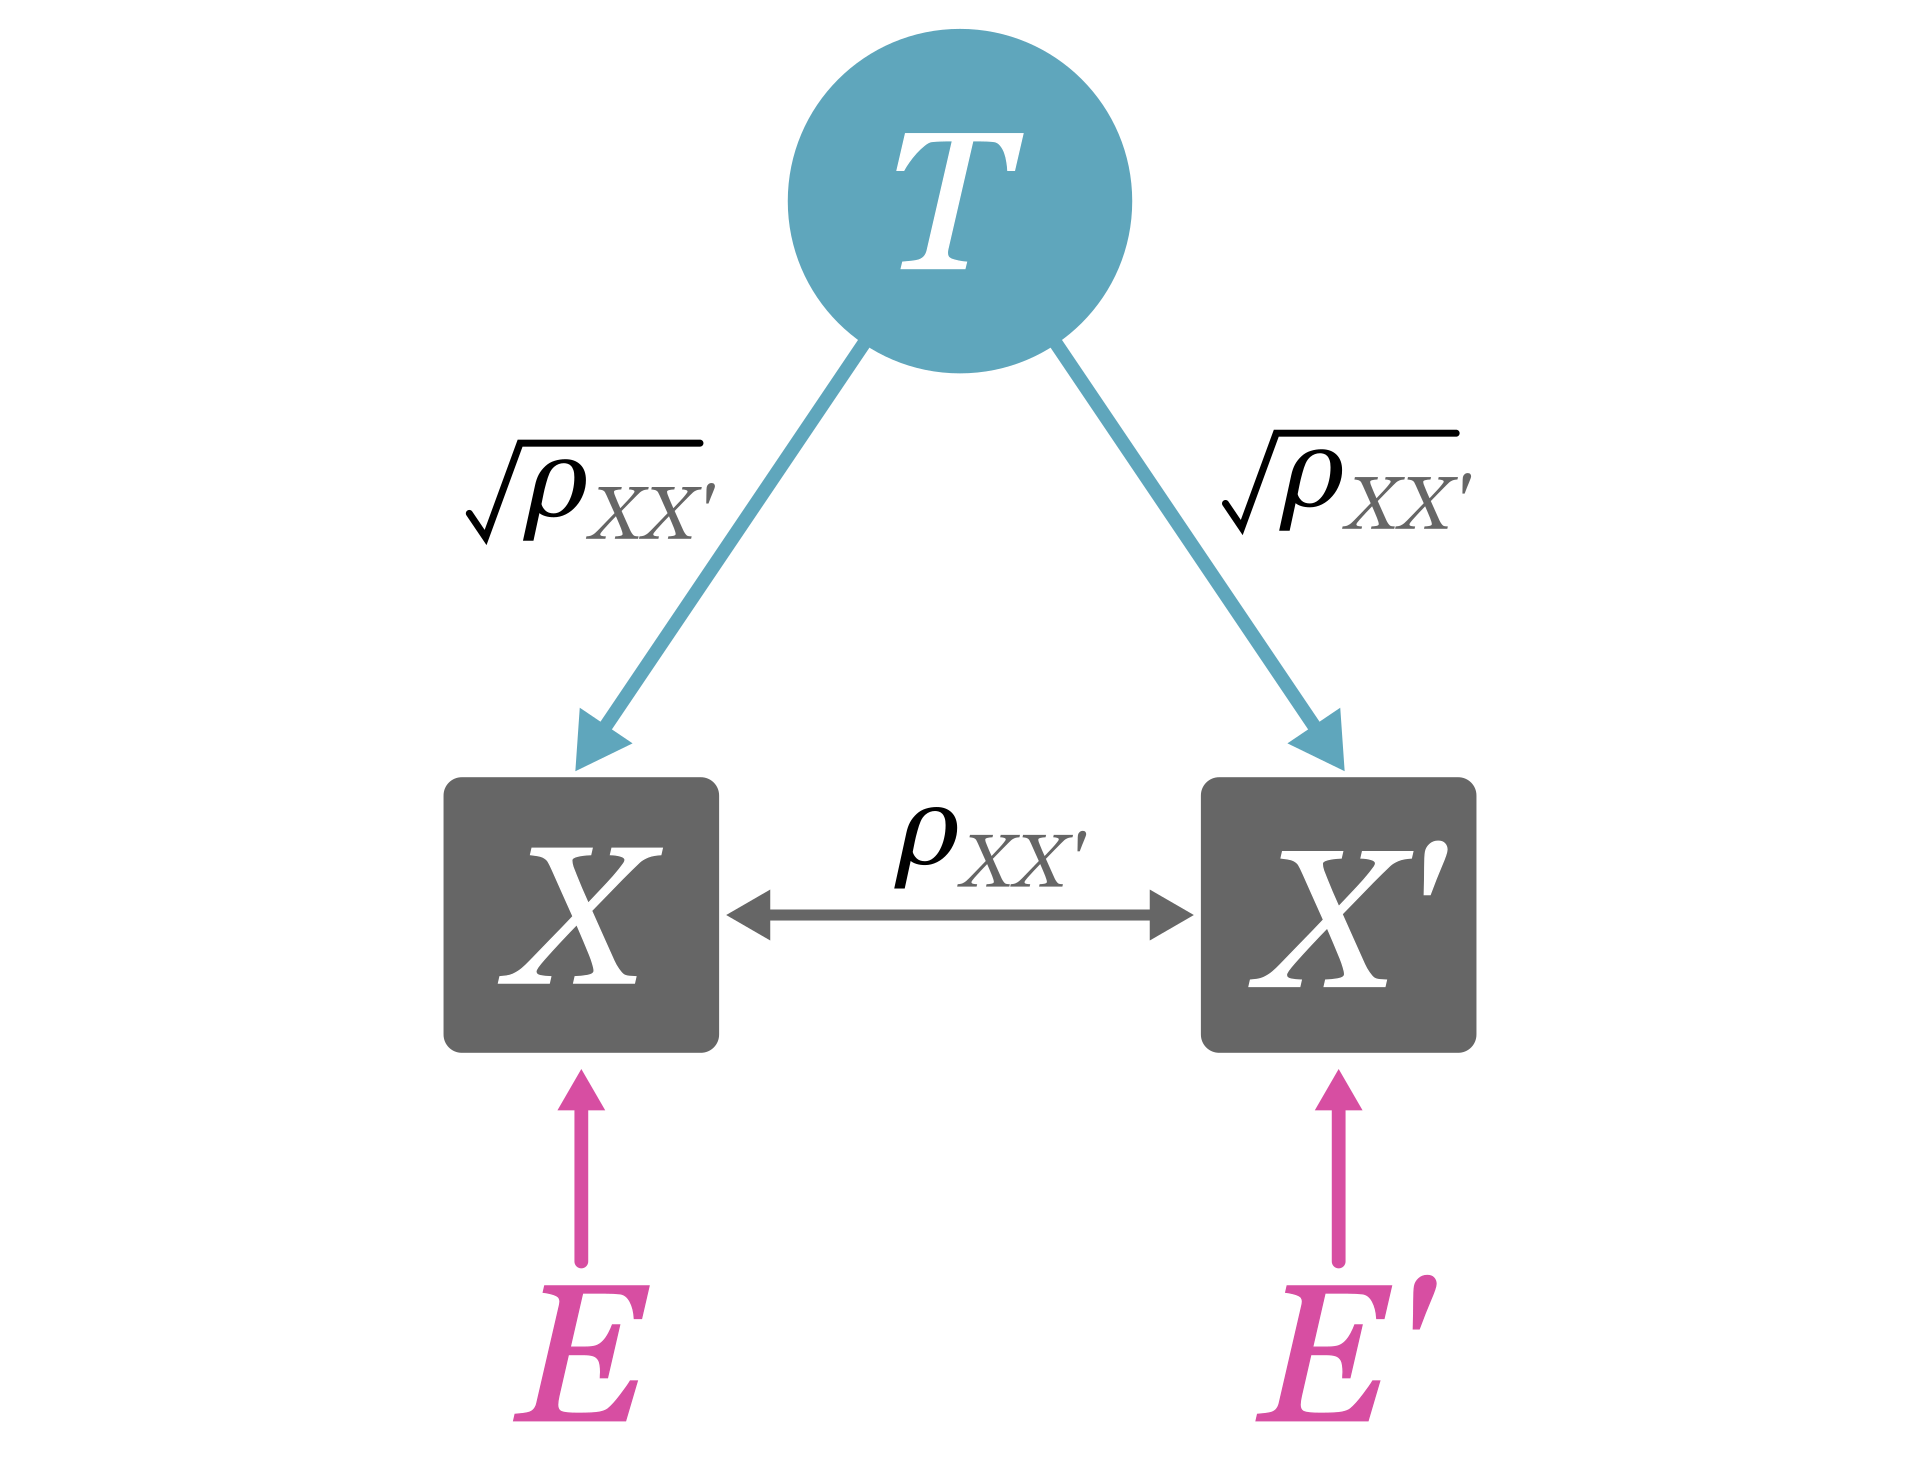
\includegraphics[width=4.16667in,height=\textheight]{chapters/04-error-in-continuous-variables/figure/unreliability_diagram_1.png}

}

\caption{\label{fig-rel}Structural diagram illustrating the relationship
between true scores, observed scores, and error scores. The pink circle
labeled \(t\) indicates the true scores, the blue squares labeled with
\(X\) and \(X'\) represent observed scores on parallel measurements, and
the red \(E\) denotes error. Correlations between \(T\), \(X\), and
\(X'\) are in terms of reliability (\(\rho_{XX'}\)). Note that
\(\rho_{XX'}=\rho_{XT}^2\).}

\end{figure}%

\section{Reliability vs Validity}\label{reliability-vs-validity}

Reliability and validity are distinct properties in measurement.
Validity pertains to whether the scores produced by a measure reflects
the quantities it is intended to measure (p.~14 Kelley 1927). According
to Borsboom, Mellenbergh, and Van Heerden (2004), a measure is
\emph{valid} if both of the following statements are true:

\begin{enumerate}
\def\labelenumi{\arabic{enumi}.}
\item
  The attribute exists.
\item
  Variations in the attribute causally produce variations in the
  outcomes of the measurement procedure.
\end{enumerate}

Borsboom's formulation of validity is simpler and more practical than
other formulations such as Cronbach and Meehl's (1955) nomological
network approach to validity. It is important to note that even if an
attribute does not exist (statement 1), scores may still provide
predictive utility. For example, socio-economic status (SES) is a
formative quantity that is constructed from a composite of education,
income, occupation status, etc. Although SES is not causal to these
indicators, SES can still be used as a predictor of important life
outcomes.

\section{Estimating Reliability}\label{estimating-reliability}

In practice, reliability must be estimated through indirect methods,
this is due to the fact that true scores and errors are unknown. There
are many reliability estimators that can be used, however we will go
over a selection of internal consistency estimators as well as
test-retest stability estimators.

\subsection{Internal Consistency
Estimators}\label{internal-consistency-estimators}

Taking multiple measurements and then averaging tends to provide a more
stable estimate of true values. For instance, let's consider the case of
Francis Galton (1907), who conducted a study involving 787 individuals
estimating the weight of an ox. On average, each person's estimate
deviated by approximately 37 pounds from the actual weight of the ox,
which was recorded as 1198 pounds. However, when all the guesses were
averaged together, the combined estimate was 1207 pounds, just a 9 pound
difference from the true value. This principle can be extended to
broader applications, such as measuring psychological constructs. If we
were to assess someone's level of extraversion using ratings from their
mother, father, friend, and sibling, the average of their combined
assessments would yield a more reliable score compared to relying solely
on a single evaluator. So to create a more stable composite score
(\(X\)), we can take the score from \(\kappa\) items (\(x\)) and sum
them such that,

\[
X = x_1 + x_2 +...+x_\kappa.
\]

The most commonly reported reliability estimator in the psychological
sciences is coefficient alpha, also referred to as Cronbach's alpha.
Coefficient alpha, along with other internal consistency estimators,
serves the purpose of assessing the reliability of composite scores
comprising multiple item scores. Coefficient alpha was first derived by
Lee Cronbach (see equation 13, Cronbach 1951) only requires three
parameters to calculate, the number of measurements (\(\kappa\)), the
sample variances of each item (\(S^2_{x_m}\)), and the variance of the
composite score (\(S^2_{X}\)). Coefficient alpha will estimate the
reliability of the composite observed score (\(r_{XX'}\)),

\begin{equation}\phantomsection\label{eq-alpha}{
_\alpha r_{XX'} = \frac{\kappa}{\kappa-1}\left( 1 - \frac{\sum_{m=1}^\kappa S^2_{x_m}}{S^2_{X}} \right).
}\end{equation}

\begin{figure}[H]

{\centering 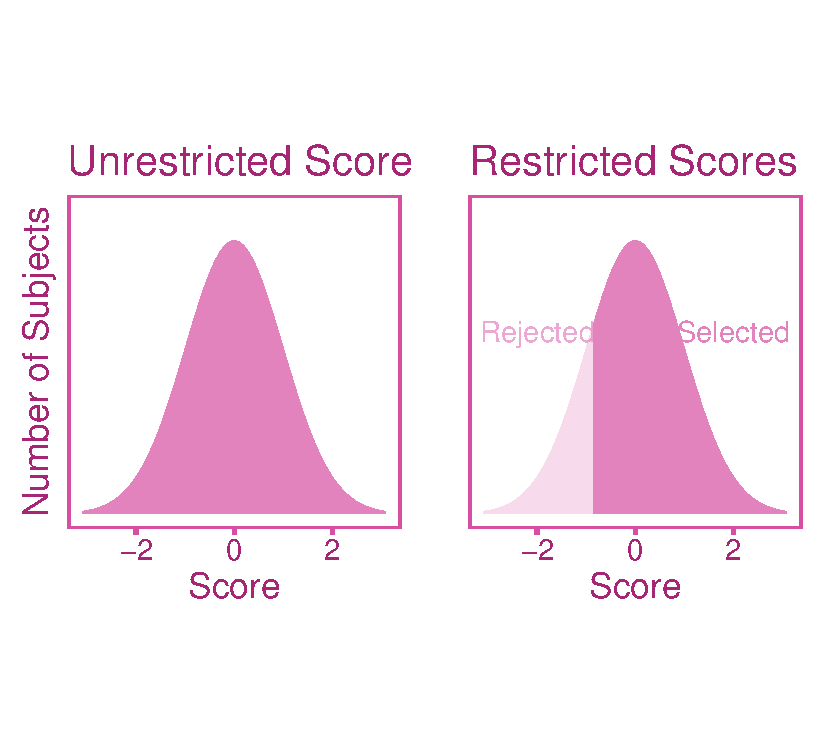
\includegraphics{chapters/04-error-in-continuous-variables/04-error-in-continuous-variables_files/figure-pdf/unnamed-chunk-1-1.pdf}

}

\caption{Figures showing the observed scores upon 10 repeated
measurements and the composite observed score for a single person (the
true score is denoted with the dashed line). The left panel shows 10
observed scores with a lot of variation (i.e., low reliability). The
composite score (dark red dot with error bars), shows wide error bars
illustrating the low precision of the observed score score. The right
panel also shows 10 observed scores with little variation (i.e., high
reliability). The composite score (dark blue dot with error bars), shows
narrow error bars illustrating the high precision of the observed
score.}

\end{figure}%

With tighter assumptions (see Haertel 2006), the formula for coefficient
alpha can be simplified to just two parameters: the number of
measurements (\(\kappa\)) and the average correlation between measured
scores (\(\bar{r}_{x_i x_j}\), where \(i\neq j\)). This formula is known
as Spearman-Brown's prophecy (see equation III of Charles Spearman 1910;
or the last equation on page 299 of Brown 1910),

\begin{equation}\phantomsection\label{eq-sp-brown}{
_\text{sb} r_{XX'}= \frac{\kappa \bar{r}_{x_i x_j}}{1+(\kappa-1)\bar{r}_{x_i x_j}}
}\end{equation}

This can be simplified further if we have two observed item scores. This
formulation is a variation of split-half reliability:

\begin{equation}\phantomsection\label{eq-split-half}{
_\text{sh}r_{XX'}= \frac{2r_{x_1 x_2}}{1+r_{x_1 x_2}}
}\end{equation}

All of these reliability estimators measure internal consistency,
therefore they do not account for error outside of the
measurement-specific error. There are other sources of error that
internal consistency reliability estimates do not account for, such as
transient error or rater-specific error.

\begin{figure}[H]

{\centering 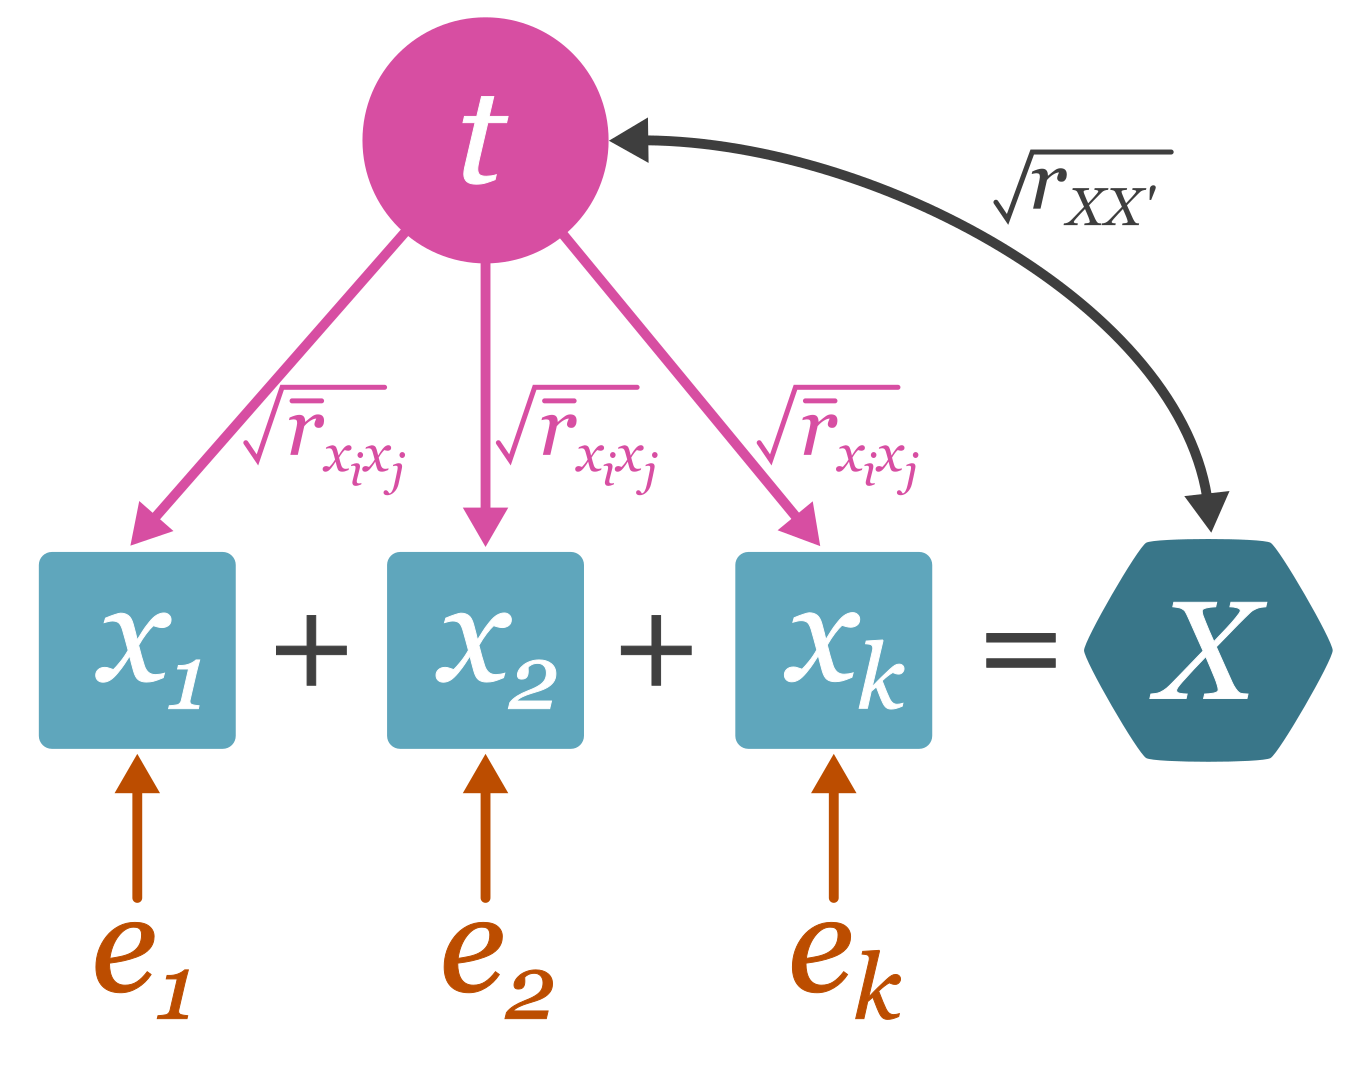
\includegraphics[width=4.16667in,height=\textheight]{chapters/04-error-in-continuous-variables/figure/unreliability_diagram_2.png}

}

\caption{Structural model illustrating internal consistency. The pink
circle labeled \(T\) indicates the true scores, the blue squares,
\(x_{1...\kappa}\), represent the observed sub-scores across multiple
measurements, and the red \(e\) denotes error. The dark blue hexagon,
\(X\), indicates a composite score as a sum of the observed scores
(\(\mathbb{x}_{1...\kappa}\)). Note that \(\rho_{XX'}=\rho_{XT}\).}

\end{figure}%

\begin{tcolorbox}[enhanced jigsaw, opacityback=0, coltitle=black, toprule=.15mm, colframe=quarto-callout-note-color-frame, bottomtitle=1mm, rightrule=.15mm, colbacktitle=quarto-callout-note-color!10!white, left=2mm, bottomrule=.15mm, breakable, title={Applied Example}, colback=white, opacitybacktitle=0.6, titlerule=0mm, arc=.35mm, leftrule=.75mm, toptitle=1mm]

Using the \texttt{anxiety} data set from the \texttt{irr} package (Gamer
et al. 2019), we can estimate the reliability of three raters evaluating
the anxiety in a sample of 20 individuals. Let us first load in the
data:

\begin{Shaded}
\begin{Highlighting}[]
\FunctionTok{library}\NormalTok{(irr)}

\CommentTok{\# load in data}
\FunctionTok{data}\NormalTok{(}\StringTok{"anxiety"}\NormalTok{, }\AttributeTok{package =} \StringTok{"irr"}\NormalTok{)}

\CommentTok{\# print data}
\FunctionTok{head}\NormalTok{(anxiety, }\DecValTok{4}\NormalTok{)}
\end{Highlighting}
\end{Shaded}

\begin{verbatim}
  rater1 rater2 rater3
1      3      3      2
2      3      6      1
3      3      4      4
4      4      6      4
\end{verbatim}

We can also use the \texttt{alpha()} function from the \texttt{psych}
package (William Revelle 2023) to estimate coefficient alpha too. The
output of \texttt{alpha} provides a lot of useful information, and it
reports two types of alphas: standardized and raw. The standardized
alpha is based on the correlations between items rather than the
covariance between items, which is useful if items are on completely
different scales (standardized alpha equivalent to the Spearman-Brown
prophecy formula found in Equation~\ref{eq-sp-brown}). Also you will
notice that the standardized alpha and ). If the ratings are on the same
scale then the raw\_alpha is preferred.

\begin{Shaded}
\begin{Highlighting}[]
\FunctionTok{library}\NormalTok{(psych)}

\NormalTok{reliability }\OtherTok{\textless{}{-}} \FunctionTok{alpha}\NormalTok{(anxiety)}

\NormalTok{rXX }\OtherTok{\textless{}{-}}\NormalTok{ reliability}\SpecialCharTok{$}\NormalTok{total}\SpecialCharTok{$}\NormalTok{raw\_alpha}

\NormalTok{rXX}
\end{Highlighting}
\end{Shaded}

\begin{verbatim}
[1] 0.4525862
\end{verbatim}

The output shows a very low reliability between raters
(\(r_{XX'}=.45\)).

\end{tcolorbox}

\subsection{Test-Retest Stability
Estimator}\label{test-retest-stability-estimator}

Transient errors represent fluctuations in observed scores over time.
These fluctuations, even if they are systematic (e.g., fatigue over the
course of a single day), add extraneous within-person variance that can
mask individual differences. Considering transient fluctuations as error
depends on the research goal, so it is important for researchers to take
care in considering which variance components should be considered error
in their study (see Section~\ref{sec-sources}). To estimate test-retest
reliability, we can compute the correlation between the measurement at
time 1 (\(X_{t_1}\)) and the second measurement at time 2 (\(X_{t_2}\)),

\[
_\text{tr}r_{XX'}= \text{corr}(X_{t_1}X_{t_2}).
\]

Note that calculating the pearson correlation coefficient between
time-points ignores systematic changes (e.g., practice effects). We can
visualize test-retest reliability in Figure~\ref{fig-test-retest} where
the top panels show the correlations between time points and the bottom
panels show the within-person change between time-points for scores with
high and low reliability.

\begin{figure}[H]

\centering{

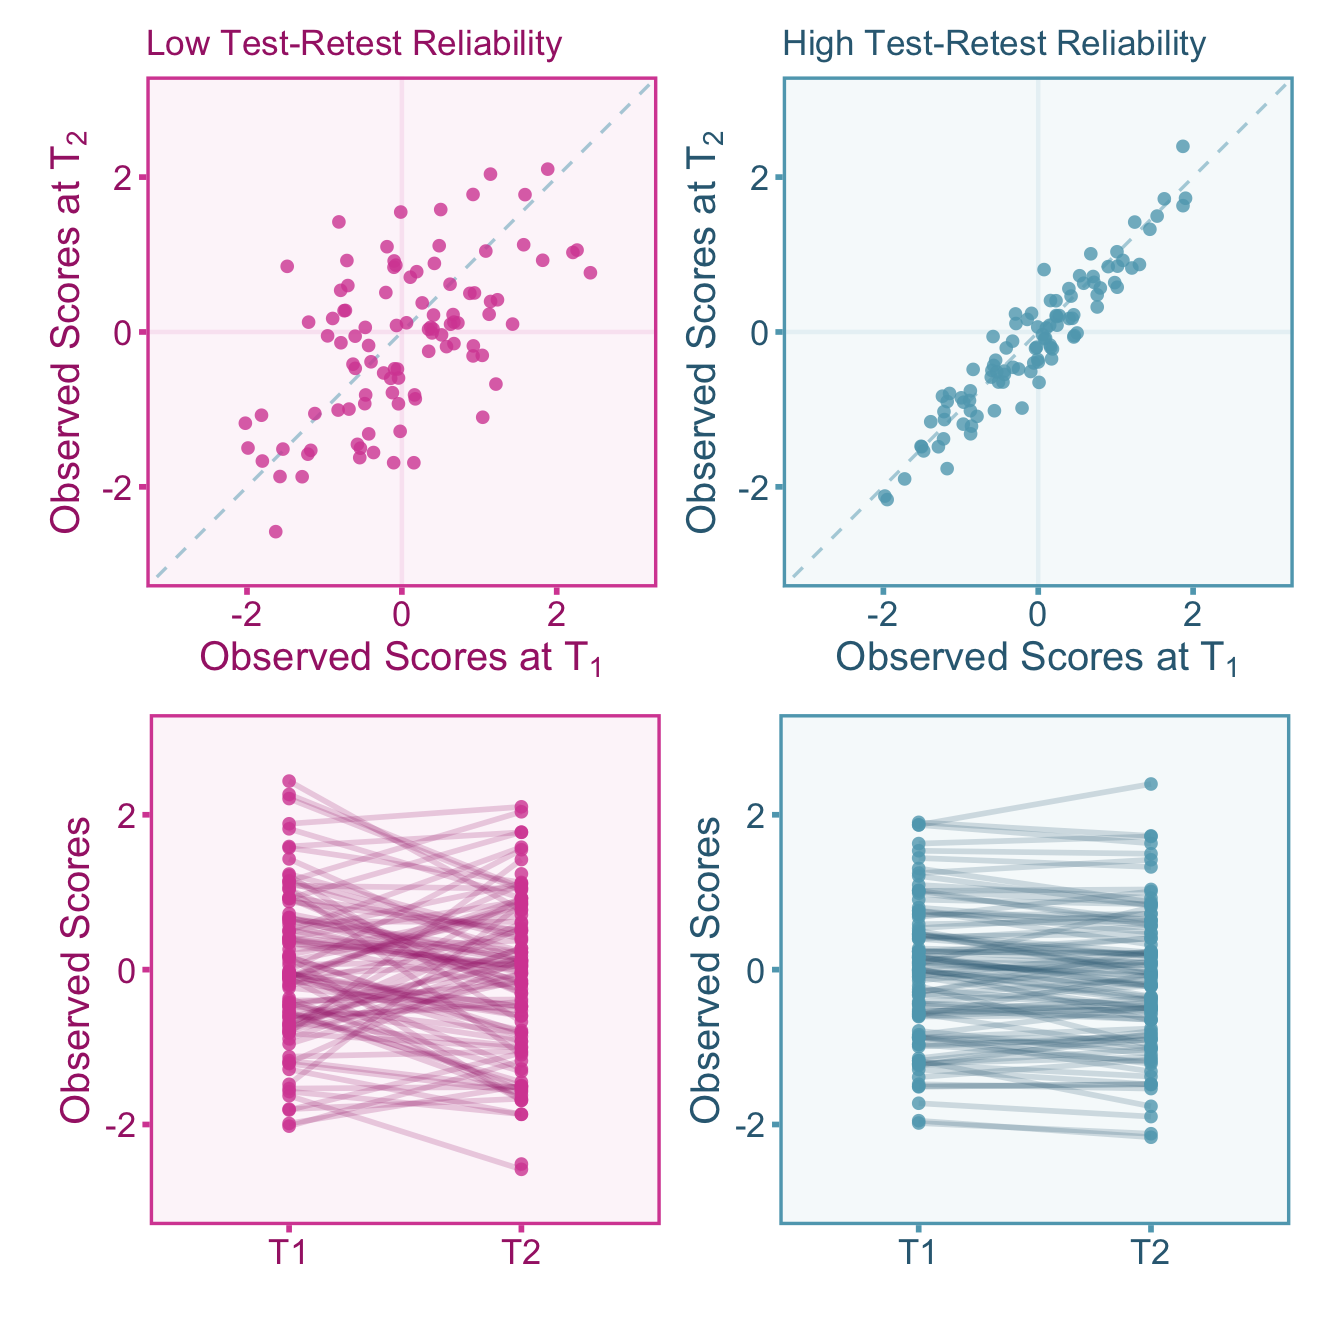
\includegraphics{chapters/04-error-in-continuous-variables/04-error-in-continuous-variables_files/figure-pdf/fig-test-retest-1.pdf}

}

\caption{\label{fig-test-retest}Illustrating test-retest reliability.
Top-left and top-right panels show the correlation between observed
scores at both time-points for a measure that has low and high
reliability, respectively. Bottom-left and bottom-right panels show the
within-person change from time-point 1 to time-point 2 for scores with
low and high reliability, respectively.}

\end{figure}%

\subsection{Sources of Measurement Error}\label{sec-sources}

Measurement error can itself be broken down into multiple sources of
error. Depending on the study, different sources of error may be more
relevant than others. Different reliability estimators will account for
different sources of error therefore it is important for researchers to
choose the right reliability estimator for their study. A description of
four of the most common sources of error is adapted from table 1 of
Wiernik and Dahlke (2020):

\begin{enumerate}
\def\labelenumi{\arabic{enumi}.}
\item
  Random Response Error: Genuine randomness in responses. Examples
  include: motor errors and variation in response time.
\item
  Time/Environment-Specific (Transient) Error: Fluctuations in scores as
  a result of the specific time or environment of the measurement. For
  instance, if researchers administered an ability test to a sample of
  undergraduate students throughout the course of a day, the student's
  who complete the test at the end of the day will likely perform worse
  than participant's who completed due to fatigue rather than ability.
  Errors due to illness, mood, hunger, environmental distractors, etc.
  all fall under the umbrella of transient errors.
\item
  Instrument-Specific Error: Error due to the specific content or
  make-up of the measurement instrument. For example, a psychological
  scale using Likert items may show participant's idiosyncratic
  interpretations of questions and response options rather than their
  standing on the latent construct.
\item
  Rater/Observer-Specific Error: Errors induced by idiosyncratic biases
  of individual raters and rater by ratee interactions (e.g., Teacher A
  gives higher grades to students who stay after class).
\end{enumerate}

Different estimators of reliability account for different sources of
measurement error therefore depending on the research design, it is
important to carefully choose which reliability is most relevant for
your use case. Note that even if two estimators account for the same
types of measurement error, they likely hold different assumptions that
may be violated in a given research context.

\begin{longtable}[]{@{}
  >{\raggedright\arraybackslash}p{(\columnwidth - 10\tabcolsep) * \real{0.1667}}
  >{\raggedright\arraybackslash}p{(\columnwidth - 10\tabcolsep) * \real{0.1667}}
  >{\centering\arraybackslash}p{(\columnwidth - 10\tabcolsep) * \real{0.1667}}
  >{\centering\arraybackslash}p{(\columnwidth - 10\tabcolsep) * \real{0.1667}}
  >{\centering\arraybackslash}p{(\columnwidth - 10\tabcolsep) * \real{0.1667}}
  >{\centering\arraybackslash}p{(\columnwidth - 10\tabcolsep) * \real{0.1667}}@{}}
\caption{List of reliability coefficients and the sources of error they
account for. The sources of error are denoted by the columns labeled
1-4, corresponding to each of the four sources of error.}\tabularnewline
\toprule\noalign{}
\begin{minipage}[b]{\linewidth}\raggedright
Estimator
\end{minipage} & \begin{minipage}[b]{\linewidth}\raggedright
Description
\end{minipage} & \begin{minipage}[b]{\linewidth}\centering
1
\end{minipage} & \begin{minipage}[b]{\linewidth}\centering
2
\end{minipage} & \begin{minipage}[b]{\linewidth}\centering
3
\end{minipage} & \begin{minipage}[b]{\linewidth}\centering
4
\end{minipage} \\
\midrule\noalign{}
\endfirsthead
\toprule\noalign{}
\begin{minipage}[b]{\linewidth}\raggedright
Estimator
\end{minipage} & \begin{minipage}[b]{\linewidth}\raggedright
Description
\end{minipage} & \begin{minipage}[b]{\linewidth}\centering
1
\end{minipage} & \begin{minipage}[b]{\linewidth}\centering
2
\end{minipage} & \begin{minipage}[b]{\linewidth}\centering
3
\end{minipage} & \begin{minipage}[b]{\linewidth}\centering
4
\end{minipage} \\
\midrule\noalign{}
\endhead
\bottomrule\noalign{}
\endlastfoot
Coefficient Alpha & Internal consistency coefficient for composite
measures. & X & & X & \\
Coefficient Omega & Internal consistency coefficient for composite
measures with specified factor structure. & X & & X & \\
Split-Half & Internal consistency coefficient for measurements that are
split into two halves. & X & & X & \\
Kuder-Richardson 20 & Internal consistency when observed scores are
binary (special case of coefficient alpha). & X & & X & \\
Item Response Theory Reliability & Reliability coefficient derived from
item response theory (as opposed to classical test theory) & X & & X
& \\
Inter-Rater/Inter-Observer Reliability & Consistency in scoring between
raters/observers. & X & & & X \\
Test-Retest & Stability coefficient for repeated measurements across
time & X & X & & \\
Delayed Alpha & Average of all possible split-half reliabilities & X & X
& X & \\
G-Coefficient & Reliability coefficient derived from generalizability
theory (G-theory). Can incorporate any source of error if enough data is
present. & X & X & X & X \\
\end{longtable}

\section{Correction for Bias in
Correlations}\label{sec-correcting-correlations-me}

\subsection{Defining the Target
Quantity}\label{defining-the-target-quantity-1}

Continuing with our emphasis on clearly defining our quantity of
interest prior to applying any corrections, let us define it here. Our
target is the population correlation between true scores of our
independent and dependent variables. We can define the observed scores
of the independent and dependent variables \(X\) and \(Y\) as,

\[
X=T+E_X
\]

\[
Y=U+E_Y.
\]

Where \(T\) and \(U\) are the true scores for the independent and
dependent variables, respectively. The population true score correlation
can thus be be denoted by, \(\rho_{TU}\), and can be defined as the
standardized covariance,

\[
\rho_{TU} = \frac{\sigma_{TU}}{\sigma_{T}\sigma_{U}}.
\]

In a given study, we will only have access to the observed scores of the
independent and dependent variables, therefore the study correlation is
\(r_{XY}\). The relationship between the observed correlation and the
true population correlation can be defined as,

\[
r_{XY} = a\rho_{TU} + \varepsilon.
\]

Where \(a\) is the artifact attenuation factor (we will see that
measurement error attenuates rather than inflates the correlation). An
unbiased estimate of the true score population correlation
(\(\rho_{TU}\)) can then be calculated by dividing the observed score
correlation by an estimate of the artifact attenuation factor,

\[
r_{TU} = \frac{r_{XY}}{\hat{a}}.
\]

The measurement model can be visualized in Figure~\ref{fig-corr-model}.

\begin{figure}[H]

\centering{

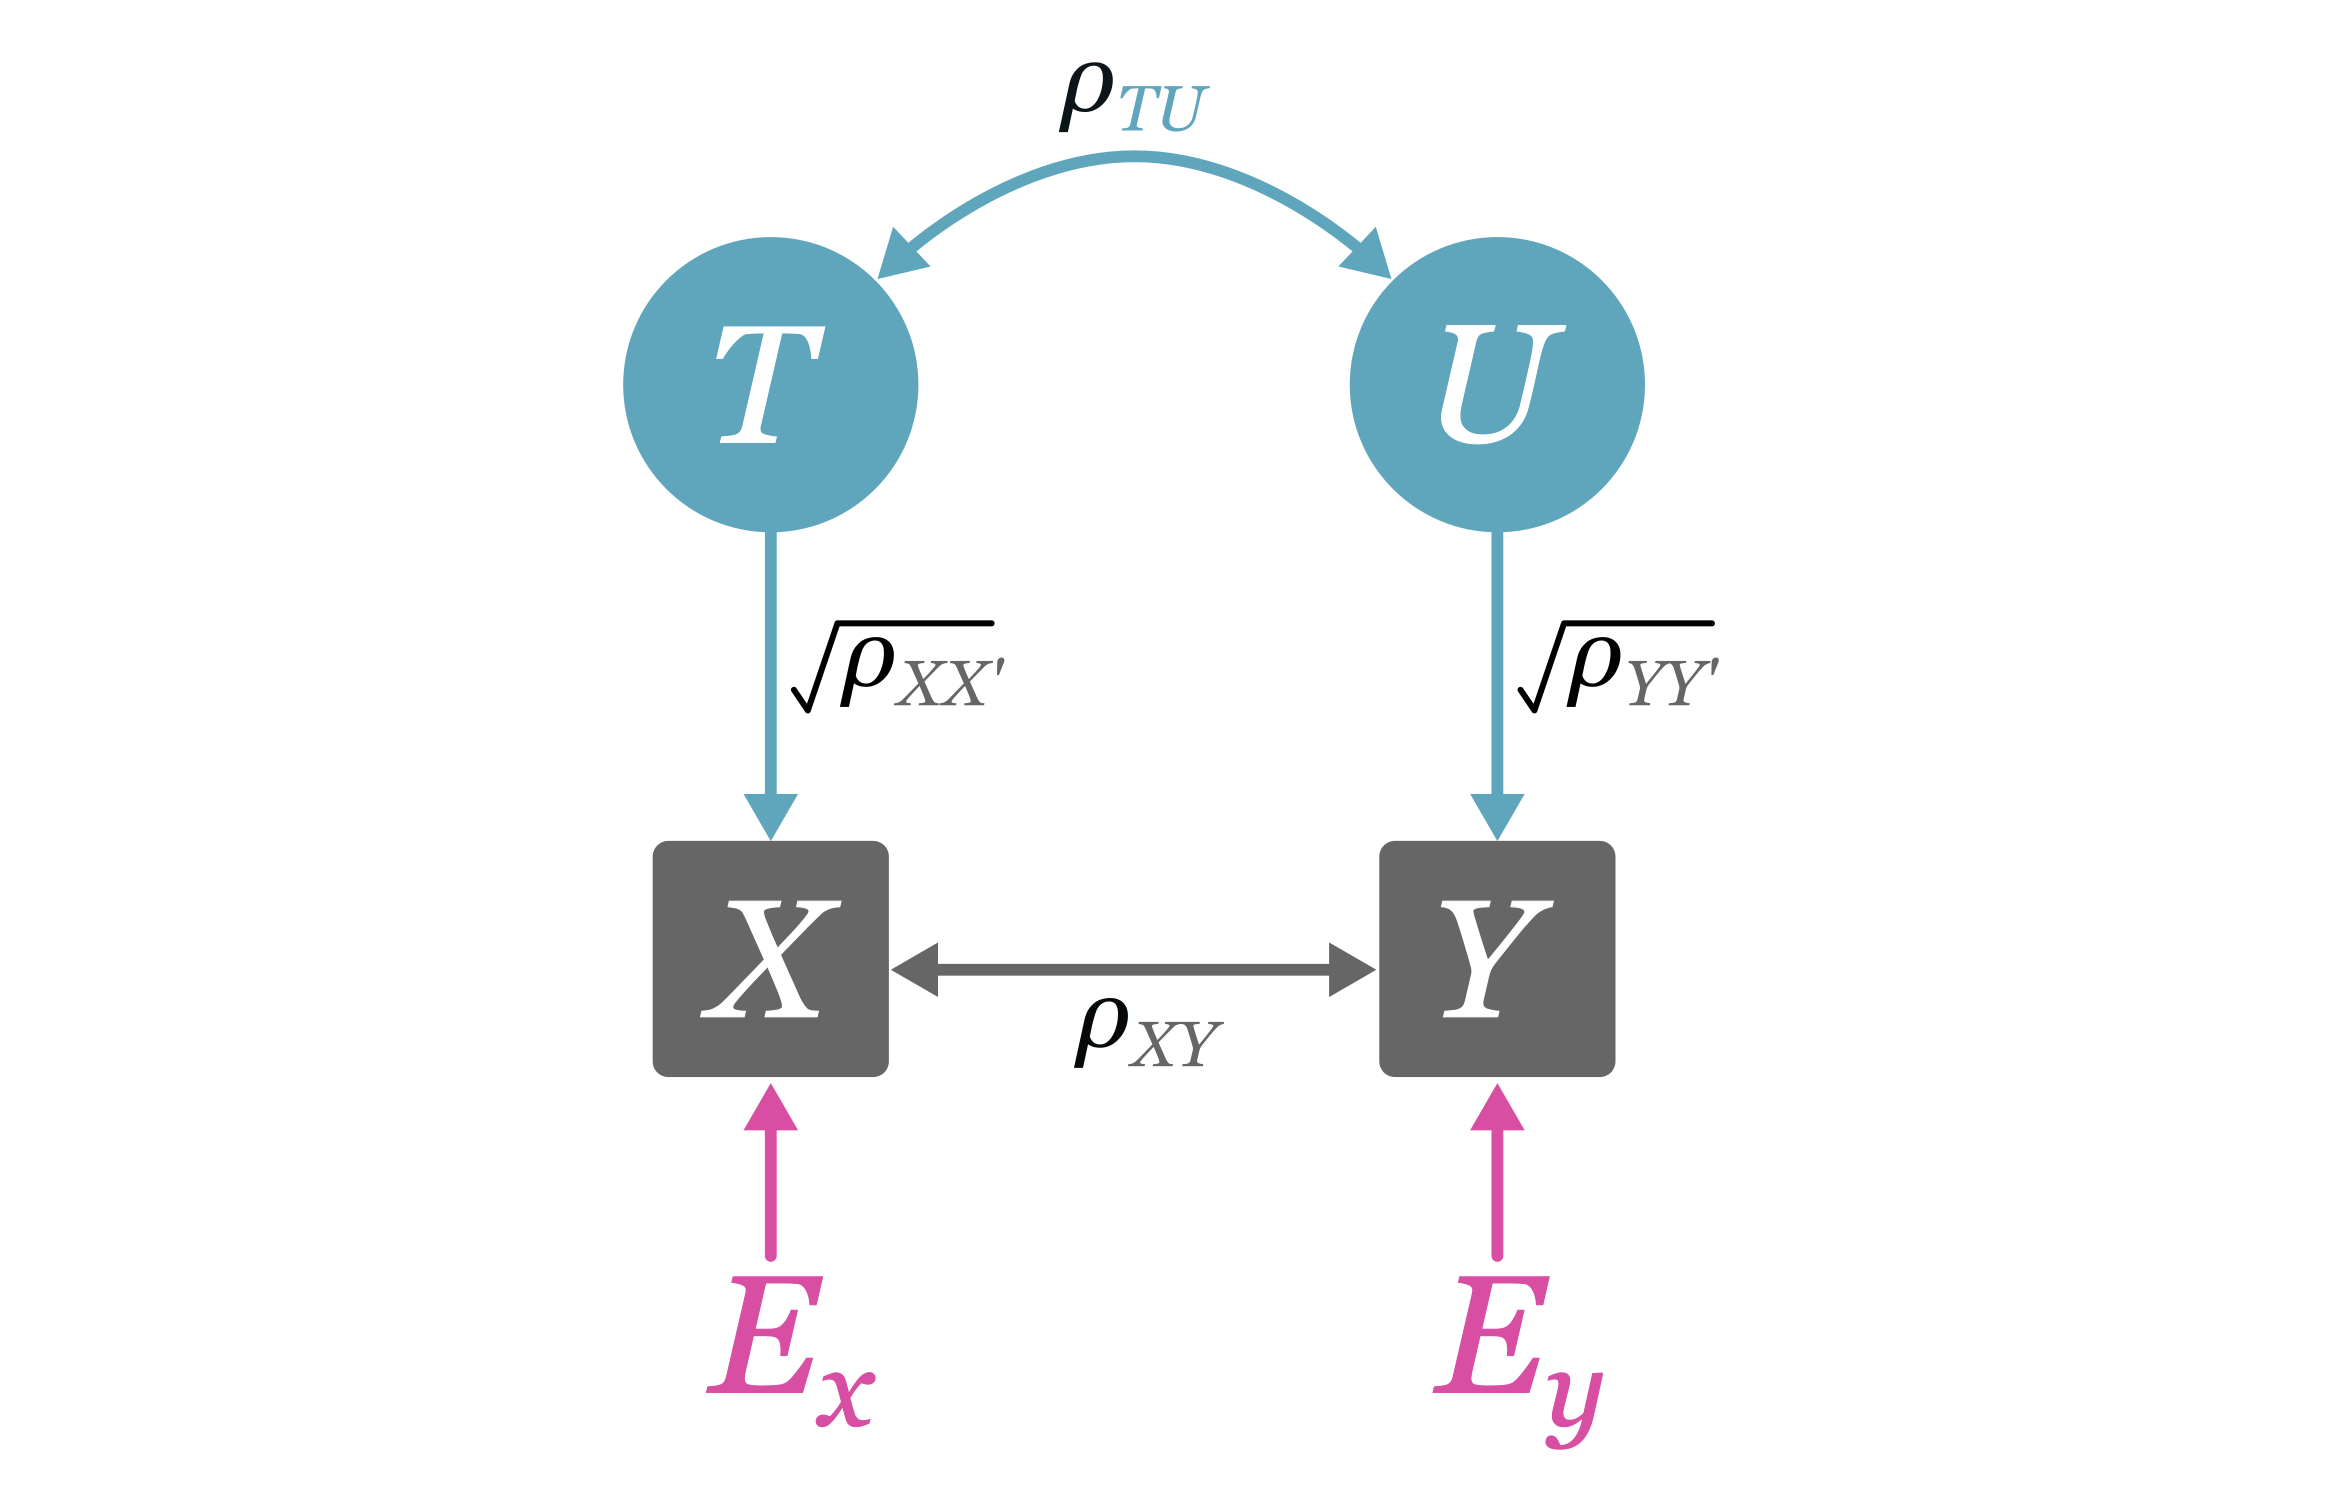
\includegraphics{chapters/04-error-in-continuous-variables/figure/diagram-estimand-reliability-r.png}

}

\caption{\label{fig-corr-model}This figure shows the relationship
between the true scores, observed scores, and error scores. The true
score correlation is denoted by the curved arrow connecting the circles
indicating true score variables, \(T\) and \(U\).}

\end{figure}%

\subsection{Artifactual Correction for Unreliability}\label{sec-r-corr}

Measurement error induces systematic bias in effect size estimates such
as correlation coefficients C. Spearman (1904). In the population, let
us assume there is some factor \(a\) that accounts for the systematic
bias in observed score correlations (\(\rho_{XY}\)) relative to true
score correlations (\(\rho_{TU}\)), such that

\[
\rho_{XY} = a \rho_{TU}.
\]

Since the correlation is defined as the covariance standardized by the
standard deviations, the population correlation between true scores,
\(T\) and \(U\), is defined as,

\[
\rho_{TU}=\frac{\sigma_{TU}}{\sigma_{T} \sigma_{U}}.
\]

Likewise the correlation between the observed scores, \(X\) and \(Y\),
would be the observed covariance divided by the observed standard
deviations,

\[
\rho_{XY} =\frac{\sigma_{XY}}{\sigma_{X} \sigma_{Y}}.
\]

However, if we assume that there is no covariance between errors in
\(X\) and \(Y\) (\(\sigma_{E_X E_Y} = 0\)), then the covariance between
observed scores is only attributable to the covariance between true
scores, therefore \(\sigma_{XY} = \sigma_{TU}\). This means that the
observed score correlation can be expressed as,

\begin{equation}\phantomsection\label{eq-bias}{
\rho_{XY} =\frac{\sigma_{TU}}{\sigma_{X} \sigma_{Y}}.
}\end{equation}

Now the only difference between the observed score correlation and the
true score correlation is the standard deviations in the denominator. In
the presence of measurement error, the observed score standard
deviations (\(\sigma_X\) and \(\sigma_Y\)) will be larger than the true
score standard deviations (\(\sigma_{T}\) and \(\sigma_{U}\)). Using the
definition of reliability, we can show how the observed variance is
inflated compared to the true variance as a function of reliability.
Since the reliability is defined as the ratio of true variance to total
observed variance (see Equation~\ref{eq-reliability}), we can see how
reliability inflates the observed variance,

\[\begin{aligned}
\sigma^2_X &=\sigma^2_{T} \left(\frac{\sigma^2_{X}}{\sigma^2_{T}} \right)\\[.3em]
&= \sigma^2_{T}\left(\frac{1}{\rho_{XX'}} \right)\\[.3em]
&= \frac{\sigma^2_{T}}{\rho_{XX'}}.
\end{aligned}\]

Therefore the observed standard deviation is,

\begin{equation}\phantomsection\label{eq-sd-me}{
\sigma_X = \frac{\sigma_{T}}{\sqrt{\rho_{XX'}}}.
}\end{equation}

Since the reliability, and its square root, will be less than 1, then
the observed score variance will be larger than the If we use the
definition of an observed score correlation (Equation~\ref{eq-bias}),
then we can replace \(\sigma_X\) and \(\sigma_Y\) with
\(\frac{\sigma_{T}}{\sqrt{\rho_{XX'}}}\) and
\(\frac{\sigma_{U}}{\sqrt{\rho_{YY'}}}\), respectively. Now we can see
how the observed score correlation differs from the true score
correlation:

\[\begin{aligned}
\rho_{XY} &= \frac{\sigma_{T U}}{\left[\frac{\sigma_{T}}{\sqrt{\rho_{XX'}}} \right] \left[ \frac{\sigma_{U}}{\sqrt{\rho_{YY'}}} \right] } \\[.3em]
&= \frac{\sigma_{T U}}{\sigma_{T}\sigma_{U}}  \sqrt{\rho_{XX'}}\sqrt{\rho_{YY'}}\\[.3em]
&= \rho_{TU} \sqrt{\rho_{XX'}}\sqrt{\rho_{YY'}} 
\end{aligned}\]

This attenuation formula was first derived by Charles Spearman (1904).
See Figure~\ref{fig-attenuation} for a visualization of the attenuation.
Note that this formulation requires that there is no correlation between
\(E_X\) and \(E_Y\) (\(\rho_{E_X E_Y}=0\)).

\begin{figure}[H]

\centering{

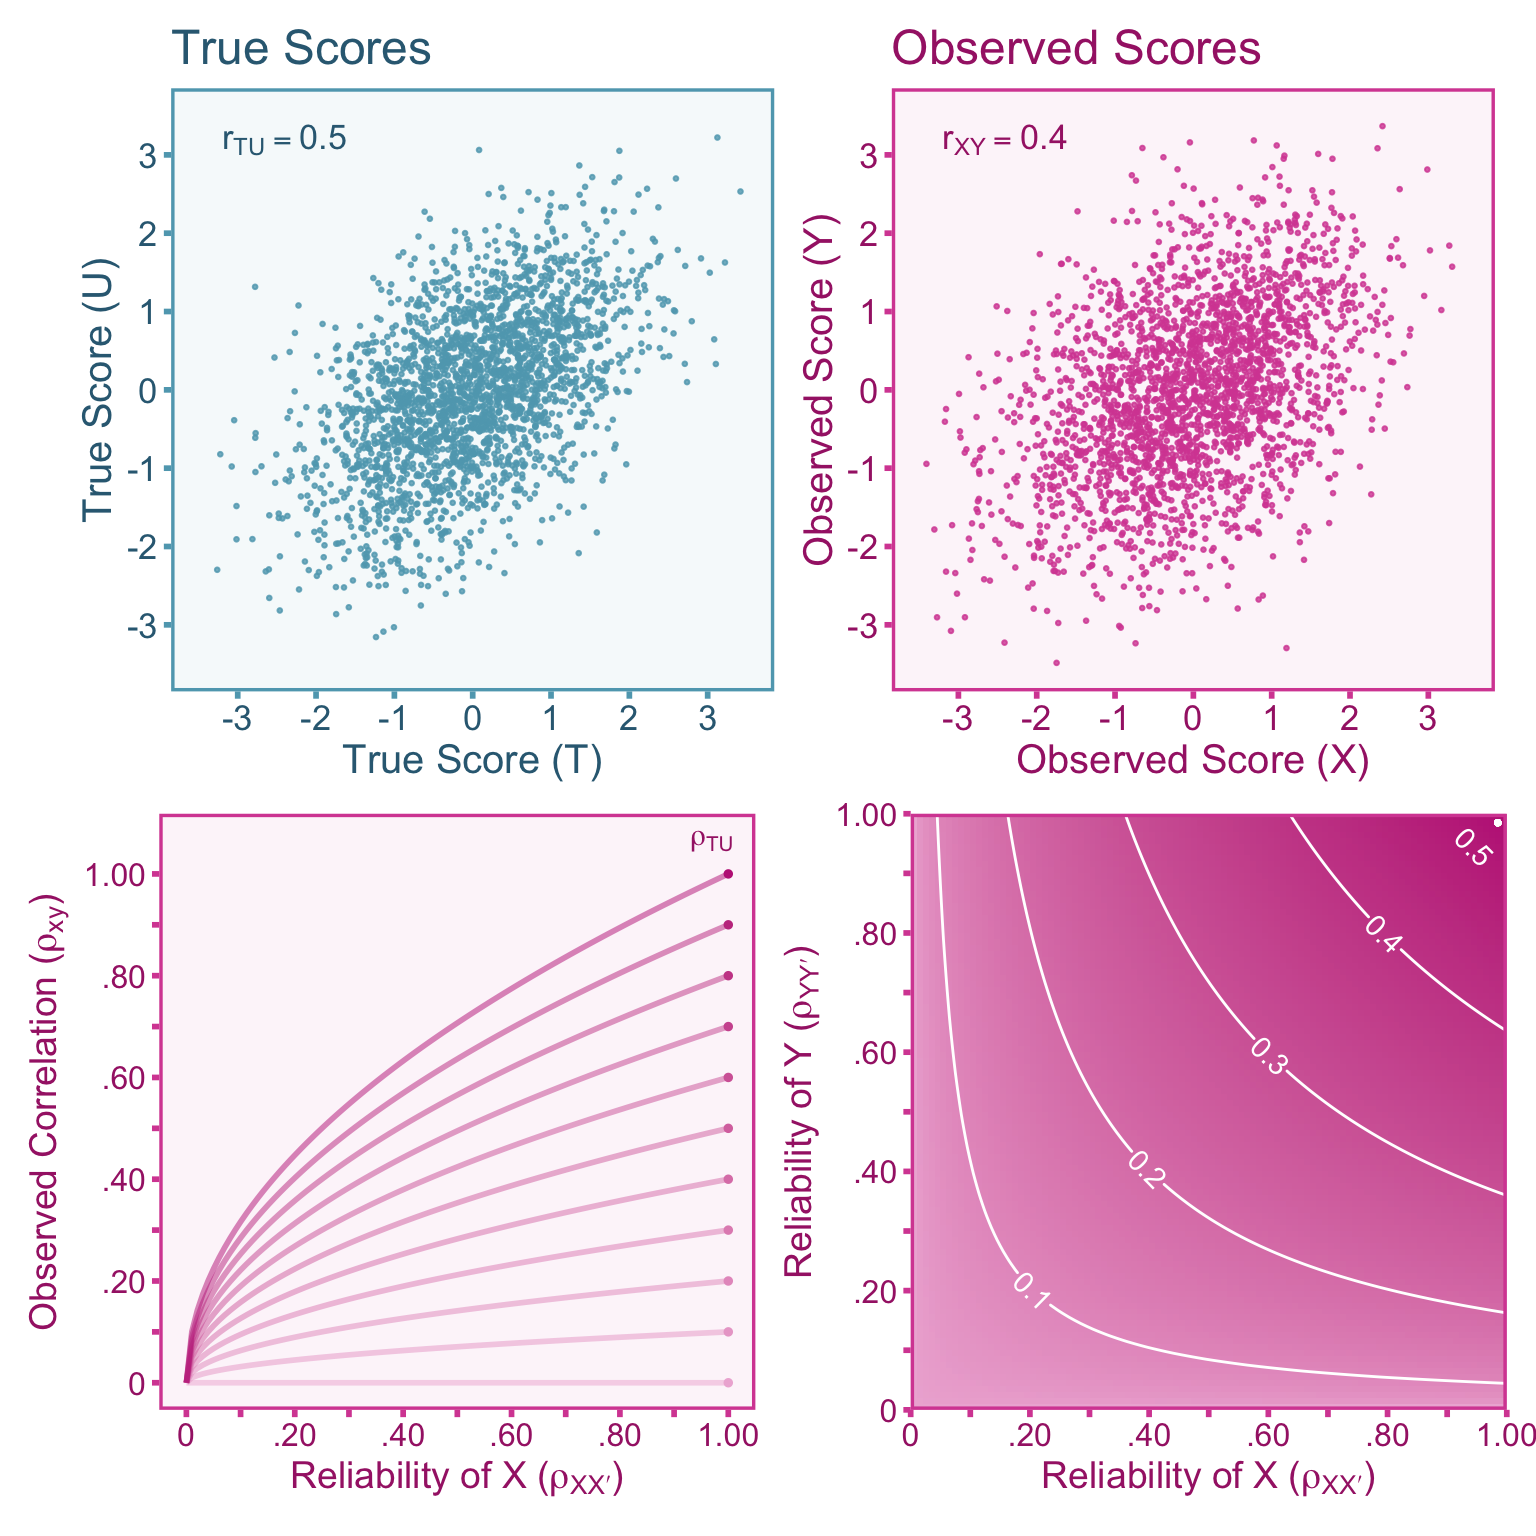
\includegraphics{chapters/04-error-in-continuous-variables/04-error-in-continuous-variables_files/figure-pdf/fig-attenuation-1.pdf}

}

\caption{\label{fig-attenuation}Visualizing the attenuation of an
observed score correlation (\(\rho_{XY}\)) due to measurement error. Top
left panel shows a scatter plot of the correlation between the true
scores of the independent (\(T\)) and dependent variable (\(U\)). Top
right panel shows a scatter plot of the correlation between the observed
scores of the independent (\(X\)) and dependent variable (\(Y\)). The
bottom left panel shows the reliability of a single variable (\(X\)) and
it's relationship with the observed score correlation (\(\rho_{XY}\))
while varying the true score correlation (true score correlations are
represented as the red dots, i.e., when reliability is perfect;
\(\rho_{TU}=\{0,.1,.2,.3,.4,.5,.6,.7,.8,.9,1.0\}\)). The bottom right
panel shows attenuation of a a true score correlation of
\(\rho_{TU}=.5\), when both \(X\) and \(Y\) are affected by measurement
error. The darker red indicates a larger observed correlation, where it
peaks at an observed score correlation of .50 (when reliability of \(X\)
and \(Y\) is 1) which is equivalent to the true score correlation}

\end{figure}%

Let us recall that we can express the observed score correlation as a
function of the true score population correlation (i.e., the target
quantity, \(\rho_{TU}\)),

\[
r_{XY} = a\rho_{TU} + e.
\]

Where \(e\) is the sampling error and \(a\) is the artifact attenuation
factor. \(a\) can now be replaced with the square root of the
reliabilities of \(X\) and \(Y\).

\[
r_{XY} = \left(\sqrt{\rho_{XX'}}\sqrt{\rho_{YY'}}\right) \rho_{TU} + e.
\]

Therefore we can correct the observed score study correlation by
dividing by an estimate the attenuation factor using,

\[
r_{TU} = \frac{r_{XY}}{\hat{a}} = \frac{r_{XY}}{\sqrt{r_{XX'}}\sqrt{r_{YY'}}}
\]

The corrected correlation coefficient is an unbiased estimator of the
target quantity, \(\rho_{TU}\). We also need to obtain the standard
error of the corrected correlation coefficient. The standard error of
the uncorrected correlation, \(se\), can be adjusted directly with one
of two formulas:

\begin{enumerate}
\def\labelenumi{\arabic{enumi}.}
\tightlist
\item
  If the reliability coefficients are estimated from the same sample as
  the correlation, then the standard error formula is,
\end{enumerate}

\[
se_c =  \frac{se}{\sqrt{r_{XX'}}\sqrt{r_{YY'}}}
\]

\begin{enumerate}
\def\labelenumi{\arabic{enumi}.}
\setcounter{enumi}{1}
\tightlist
\item
  If the reliability coefficients and the correlation are all estimated
  from different samples (\(n\) will denote the sample size of the
  standardized mean difference, \(n_{r_{XX'}}\) and \(n_{r_{YY'}}\) and
  will denote the sample size of the respective reliability
  coefficients) then the standard error of the corrected correlation is
  approximately (for the derivation, see the appendix of this section),
\end{enumerate}

\begin{equation}\phantomsection\label{eq-se-me-r-tsa}{
se(r_{TU}) = \sqrt{\frac{se(r_{XY})^2}{r_{XX'}r_{YY'}} + 
\frac{r^2_{XY}\left(1-r^2_{XX'}\right)^2}{4(n_{r_{XX'}}-1)r_{XX'}^3r_{YY'}} + 
\frac{r^2_{XY}\left(1-r^2_{YY'}\right)^2}{4(n_{r_{YY'}}-1)r_{XX'}r_{YY'}^3}}
}\end{equation}

The two ways of calculating standard error are due to the fact that when
the reliability and correlation coefficient are computed from the same
sample, their sampling errors will be correlated (Bobko and Rieck 1980).
Note that if you only want to correct for unreliability in one variable,
than you can set the reliability of the other variable to 1 in all the
equations above.

\begin{tcolorbox}[enhanced jigsaw, opacityback=0, coltitle=black, toprule=.15mm, colframe=quarto-callout-note-color-frame, bottomtitle=1mm, rightrule=.15mm, colbacktitle=quarto-callout-note-color!10!white, left=2mm, bottomrule=.15mm, breakable, title={Applied Example in R}, colback=white, opacitybacktitle=0.6, titlerule=0mm, arc=.35mm, leftrule=.75mm, toptitle=1mm]

Let's say we wanted to estimate the correlation between academic
motivation and test performance among a sample of \(n=100\) students.
Motivation scores are obtained using a self-report measure with a
reliability of \(r_{XX'}=.80\). Test performance is the sum of correctly
answered multiple choice questions and the total scores were also fairly
reliable (\(r_{YY'}=.80\)). The correlation between observed motivation
and performance scores is \(r_{XY}=.40\). To correct the correlation for
measurement error, we can use the \texttt{correct\_r} function in the
\texttt{psychmeta} package (Dahlke and Wiernik 2019).

\begin{Shaded}
\begin{Highlighting}[]
\FunctionTok{library}\NormalTok{(psychmeta)}

\NormalTok{rXY }\OtherTok{\textless{}{-}}\NormalTok{ .}\DecValTok{40}  \CommentTok{\# correlation between X and Y}
\NormalTok{rXX }\OtherTok{\textless{}{-}}\NormalTok{ .}\DecValTok{80}  \CommentTok{\# reliability of X}
\NormalTok{rYY }\OtherTok{\textless{}{-}}\NormalTok{ .}\DecValTok{80}  \CommentTok{\# reliability of Y}
\NormalTok{n }\OtherTok{\textless{}{-}} \DecValTok{100}    \CommentTok{\# sample size}

\CommentTok{\# correct correlation}
\FunctionTok{correct\_r}\NormalTok{(}\AttributeTok{correction =} \StringTok{\textquotesingle{}meas\textquotesingle{}}\NormalTok{,}
          \AttributeTok{rxyi =}\NormalTok{ rXY,}
          \AttributeTok{rxx =}\NormalTok{ rXX,}
          \AttributeTok{ryy =}\NormalTok{ rYY,}
          \AttributeTok{n =}\NormalTok{ n)}
\end{Highlighting}
\end{Shaded}

\begin{verbatim}
Correlations Corrected for Measurement Error:
---------------------------------------------------------------------------------------
  value CI_LL_95 CI_UL_95   n n_effective
1   0.5    0.276    0.691 100        51.5
\end{verbatim}

The estimate of the true score correlation is
\(r_{TU} = .50\;[.28, .69]\).

\end{tcolorbox}

\section{\texorpdfstring{Correction for Bias in Standardized Mean
Differences
(\emph{d})}{Correction for Bias in Standardized Mean Differences (d)}}\label{correction-for-bias-in-standardized-mean-differences-d}

\subsection{Defining the Target
Quantity}\label{defining-the-target-quantity-2}

Prior to correcting for measurement error let us define our target. Our
target is the difference in the means of group \(A\) and \(B\) with
respect to the true scores, \(U\), of our dependent variable, \(Y\),

\[
Y_A = U_A + E_A
\]

\[
Y_B = U_B + E_B.
\]

Where \(U_A\) and \(U_B\) are the true scores for group \(A\) and group
\(B\), respectively. The true score standardized mean difference can
thus be be denoted by, \(\delta_{gU}\) (\(g\) indicates the grouping
variable, and \(U\) denotes the continuous true score outcome), and can
be defined as the mean difference divided by the within-group standard
deviation,

\[
\delta_{gU} = \frac{\mu_{U_A} - \mu_{U_B}}{\sigma_{U}}.
\]

Where \(\mu_U\) indicates the population mean of true scores. The
relationship between the population true score standardized mean
difference (\(\delta_{gU}\)) can be related to the observed study
standardized mean difference with the following formulation:

\[
d_{gY} = a\delta_{gU}+e.
\]

Where \(a\) is the attenuation factor induced by measurement error and
\(e\) denotes sampling error. To obtain an unbiased estimate of true
score standardized mean difference, \(\delta_{gU}\), we can correct the
observed standardized mean difference by dividing by an estimate of
\(a\),

\[
d_{gU} = \frac{d_{gY}}{\hat{a}}.
\]

\subsection{Artifact Correction for Unreliability}\label{sec-d-SMD}

The population mean of true scores and observed scores are identical
since measurement error only affects the variance in scores. Therefore
the population mean difference is equal between true and observed
scores:

\[
\mu_{U_A} - \mu_{U_B} = \mu_{Y_A} - \mu_{Y_B}
\]

Note that this means that an unstandardized mean difference is
\emph{not} biased by measurement error. Since the mean difference in
true scores and observed scores are the same, the observed score
population standardized mean difference can also be expressed as the
mean difference of true scores standardized by the observed score
standard deviation,

\[
\delta_{gY} = \frac{\mu_{Y_A} - \mu_{Y_B}}{\sigma_Y}  = \frac{\mu_{U_A} - \mu_{U_B}}{\sigma_Y}
\]

We know from Equation~\ref{eq-reliability} that the standard deviation
of true scores, \(\sigma_U\), can be expressed as a function of
reliability and the observed score standard deviation,

\begin{equation}\phantomsection\label{eq-sd-correction}{
\sigma_U = \sigma_Y\sqrt{\rho_{YY'}}
}\end{equation}

Therefore the true score standardized mean difference could be corrected
for by dividing the observed score standardized mean difference by the
reliability,

\[
\delta_{gU} = \frac{\mu_{U_A} - \mu_{U_B}}{\sigma_Y\sqrt{\rho_{YY'}}} = \frac{\delta_{gY}}{\sqrt{\rho_{YY'}}}
\]

The reliability in this case is the within-group reliability
(\(\rho_{YY'}=\rho_{YY'_A}=\rho_{YY'_B}\)) which is assumed to be equal
between groups. Similarly, a sample estimator of the observed score
standardized mean difference can be expressed as,

\[
d_{gY} = \frac{\overline{Y}_A - \overline{Y}_B}{S_{Y_P}}  = \frac{\overline{U}_A - \overline{U}_B}{S_{Y_P}}
\]

Where \(\overline{Y}\) and \(\overline{U}\) are sample means of observed
scores and true scores, respectively. The within-group standard
deviation of observed scores can be estimated by pooling the standard
deviation from both groups,

\[
S_{Y_P} = \sqrt{\frac{(n_A+1)S^2_{Y_A}+(n_B+1)S^2_{Y_B}}{n_A + n_B - 2}}.
\]

Where \(n_A\) and \(n_B\) are the sample sizes within group \(A\) and
group \(B\), respectively.

\subsubsection*{Pooled Reliability}\label{pooled-reliability}
\addcontentsline{toc}{subsubsection}{Pooled Reliability}

To obtain the pooled standard deviation of true scores, we can correct
the observed score standard deviations for measurement error such that,
\(S^2_{Y}=r_{YY'}S^2_{U}\) (similar to what we see in
Equation~\ref{eq-sd-correction}). Therefore we can compute the pooled
true score standard deviation (\(S_{U_P}\)) with,

\[
S_{U_P} = \sqrt{\frac{(n_A+1)\left(S_{Y_A} \sqrt{r_{YY'_A}}\right)^2+(n_B+1)\left(S_{Y_B} \sqrt{r_{YY'_B}}\right)^2}{n_A + n_B - 2}}.
\]

Alternatively, we can pool the reliability and the true score standard
deviations separately,

\[
S_{Y_P} = \sqrt{\frac{(n_A+1)S_{Y_A}^2+(n_B+1)S_{Y_B}^2}{n_A + n_B - 2}}
\]

\[
r_{YY'_P} = \sqrt{\frac{(n_A+1) r_{YY'_A}^2+(n_B+1)r_{YY'_B}^2}{n_A + n_B - 2}}.
\]

Then we can express \(S_{U_P}\) as the pooled standard deviation and the
pooled reliability,

\[
S_{U_P} = S_{Y_P}\sqrt{r_{YY'_P}}.
\]

Now we can calculate the corrected sample standardized mean difference,
so that it estimates the standardized mean difference in true scores
rather than observed scores:

\[
d_{gU} = \frac{\overline{U}_A - \overline{U}_B}{S_{U_P}} =  \frac{\overline{U}_A - \overline{U}_B}{S_{Y_P}\sqrt{r_{YY'_P}}} = \frac{d_{gY}}{\sqrt{r_{YY'_P}}}
\]

The corrected (true score) standardized mean difference, \(d_{gU}\),
will also need it's standard error to be adjusted from the observed
score estimate. The standard error can be computed one of two ways:

\begin{enumerate}
\def\labelenumi{\arabic{enumi}.}
\tightlist
\item
  If the reliability coefficient and the standardized mean difference
  are computed from the same sample then the standard error can be
  estimated by, \[
  se(d_{gU}) = \frac{se(d_{gY})}{\sqrt{r_{YY'_P}}}.
  \]
\item
  If the reliability coefficient and the standardized mean difference
  are computed from separate samples (\(n\) will denote the sample size
  of the standardized mean difference, \(n_{r_{YY'}}\) and will denote
  the sample size of the reliability coefficient), we can use the
  following formulation (see appendix for derivation),
\end{enumerate}

\begin{equation}\phantomsection\label{eq-se-me-d-tsa}{
se(d_{gU}) = \sqrt{\frac{se(d_{gY})^2}{r_{YY'_P}} +\frac{d^2_{gY}\left(1-r^2_{YY'_P}\right)^2}{4\left(1-n_{r_{YY'_P}}\right)r^3_{YY'_P}}}
}\end{equation}

\subsubsection*{Total Sample
Reliability}\label{total-sample-reliability}
\addcontentsline{toc}{subsubsection}{Total Sample Reliability}

It is common that studies will only report the full sample reliability
and not the reliability within each group. If the groups differ
substantially on the dependent variable, \(Y\), then the total sample
reliability will over-estimate the within-group reliability. When the
total sample reliability is all that is available, we can correct the
standardized mean difference by first converting \(d_{gY}\) to a
point-biserial correlation, \(r_{gY}\). To do this we also need the
observed proportion of subjects in group \(A\) \emph{or} \(B\) (\(p_g\)
; it does not matter which group is chosen, as long as it is consistent
throughout).

\[
r_{gY} = \frac{d_{gY}}{\sqrt{\frac{1}{p_g(1-p_g)}+d_{gY}^2}}.
\]

Then we can the correlation coefficient as we did in
Section~\ref{sec-r-corr}. Taking the reliability of \(Y\), the
\(r_{gY}\) for the total sample reliability (see
Section~\ref{sec-correcting-correlations-me} for details),

\[
r_{gU} = \frac{r_{gY}}{\sqrt{r_{YY'}}}
\]

Then we can obtain the corrected (true score) standardized mean
difference by converting \(r_{gU}\) back into \(d_{gU}\),

\[
d_{gU} = \frac{r_{gU}}{\sqrt{p_g(1-p_g)(1-r_{gU}^2)}}
\]

The standard error of the corrected value will also need to be adjusted.
The same process can be done for the sampling variance as well, but
instead we can put it all into one equation,

\[
se_{c} = \frac {se\left(\frac{r_{gU}}{r_{gY}}\right)} {\sqrt{\left(1+d_{gY}^2p_g[1-p_g]\right)^3\left(1-r_{gU}^2\right)^3}}
\]

Note that this formula is specifically for the case where the
standardized mean difference and the reliability coefficient are
estimated from the same sample. If they are estimated from separate
samples, then we can convert the standard error of the standardized mean
difference to a standard error of a point-biserial correlation and then
use Equation~\ref{eq-se-me-r-tsa}. Once the point-biserial standard
error is corrected, then it can be converted back to a correlation
coefficient.

\begin{figure}[H]

\centering{

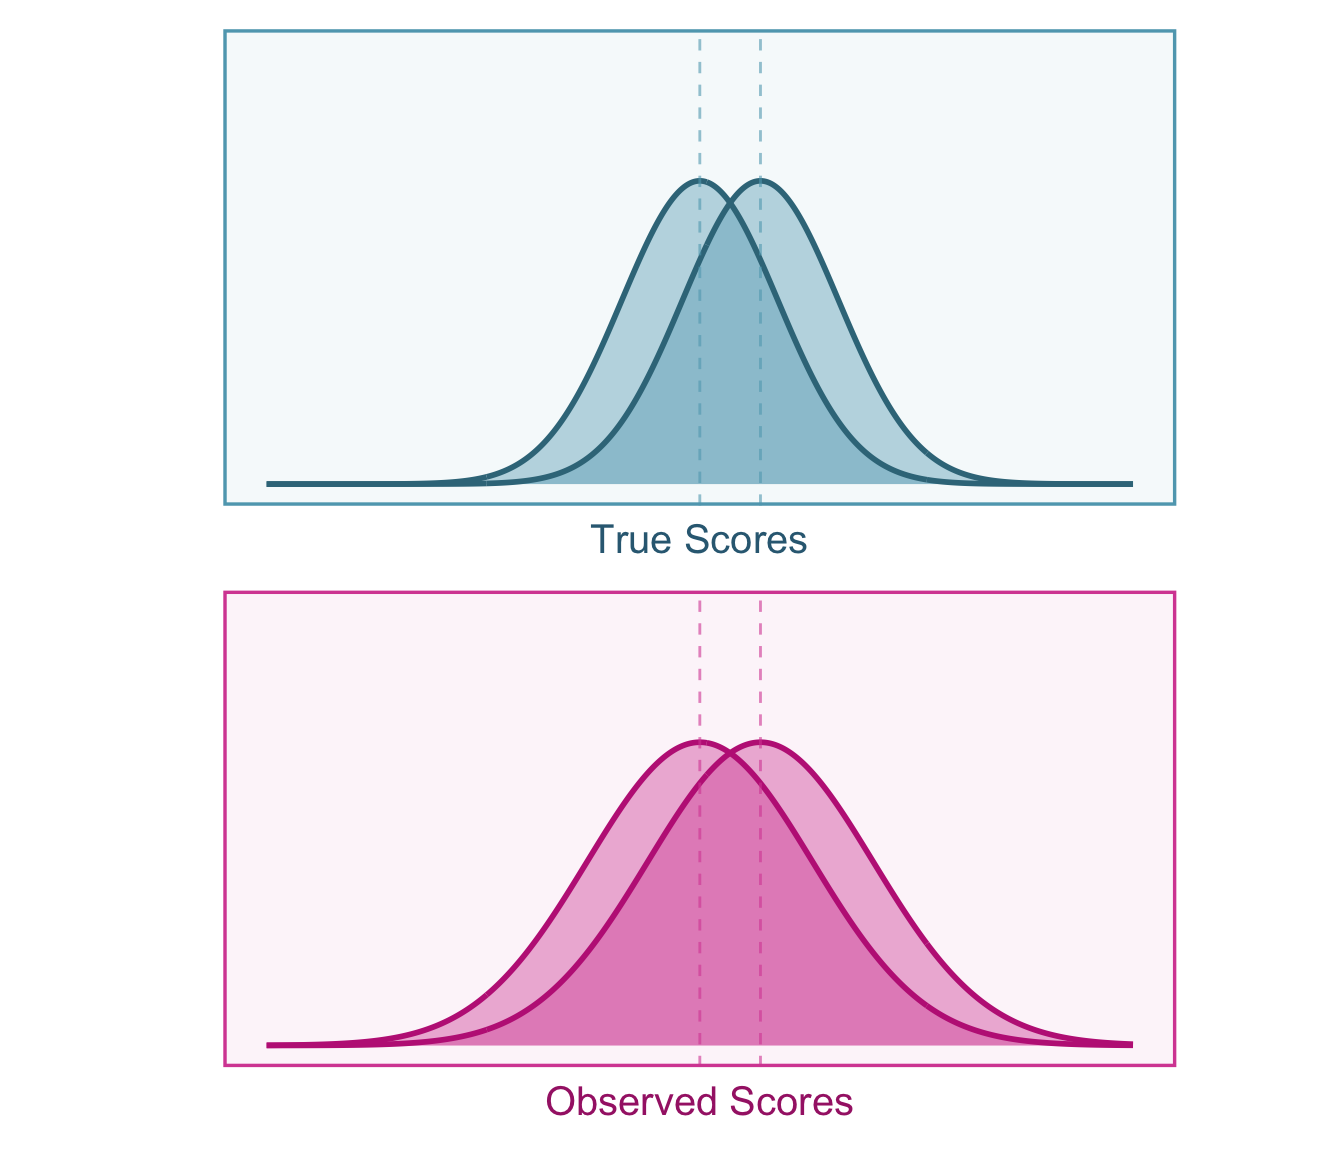
\includegraphics{chapters/04-error-in-continuous-variables/04-error-in-continuous-variables_files/figure-pdf/fig-d-attenuation-1.pdf}

}

\caption{\label{fig-d-attenuation}Visualizing the attenuation of the
standardized mean differences in observed scores (bottom panel) from
true scores (top panel). The true score standardized mean difference is
\(\delta_{gU}=0.60\), but in the presense of measurement error
(\(\rho_{YY'}=.70\)) the observed score standardized mean difference is
\(\delta_{gY}=0.50\). This occurs due to the increased standard
deviation in observed scores relative to true scores (the mean
difference does not change).}

\end{figure}%

\begin{tcolorbox}[enhanced jigsaw, opacityback=0, coltitle=black, toprule=.15mm, colframe=quarto-callout-note-color-frame, bottomtitle=1mm, rightrule=.15mm, colbacktitle=quarto-callout-note-color!10!white, left=2mm, bottomrule=.15mm, breakable, title={Applied Example in R}, colback=white, opacitybacktitle=0.6, titlerule=0mm, arc=.35mm, leftrule=.75mm, toptitle=1mm]

Imagine we want to test the effectiveness of a drug that is meant to
alleviate stress. Therefore we conduct a study and randomize a sample of
150 people into a control group (\(n=75\)) and a treatment group
(\(n=75\)). After the intervention, the subjects report their stress
levels on a self-report scale. The scale was shown to have a reliability
of \(r_{YY'}=.80\). We can correct the standardized mean differences on
observed scores with the \texttt{correct\_d} function in the
\texttt{psychmeta} package (Dahlke and Wiernik 2019).

\begin{Shaded}
\begin{Highlighting}[]
\FunctionTok{library}\NormalTok{(psychmeta)}

\NormalTok{dgY }\OtherTok{\textless{}{-}}\NormalTok{ .}\DecValTok{40}
\NormalTok{rYY }\OtherTok{\textless{}{-}}\NormalTok{ .}\DecValTok{80}
\NormalTok{n1 }\OtherTok{\textless{}{-}}\NormalTok{ n2 }\OtherTok{\textless{}{-}} \DecValTok{75}

\FunctionTok{correct\_d}\NormalTok{(}\AttributeTok{correction =} \StringTok{\textquotesingle{}meas\textquotesingle{}}\NormalTok{,}
          \AttributeTok{d =}\NormalTok{ dgY,}
          \AttributeTok{ryy =}\NormalTok{ rYY,}
          \AttributeTok{n1 =}\NormalTok{ n1,}
          \AttributeTok{n2 =}\NormalTok{ n2)}
\end{Highlighting}
\end{Shaded}

\begin{verbatim}
d Values Corrected for Measurement Error:
---------------------------------------------------------------------------------------
  value CI_LL_95 CI_UL_95   n n_effective
1 0.449   0.0828    0.838 150         118
\end{verbatim}

The output of psychmeta shows a slightly larger
(\(d_{gU} = 0.45\,[0.08,0.84]\)).

\end{tcolorbox}

\section{Estimating Reliability with Limited
Information}\label{sec-lim-information}

Reliability estimates should preferably be calculated from within the
study's sample, however there are a couple of ways to estimate
reliability when this information is not provided. A common way to
obtain an estimate of the reliability is to look in meta-analyses or a
test manuals. If the number of items in a study differs from the test
manual, you can approximate the reliability of the study's test, with a
re-arrangement of the Spearman-Brown prophecy formula,

\[
r_{xx'_{study}} \approx \frac{1}{\frac{\kappa_{\text{ref}}}{\kappa_{\text{study}}} \left(\frac{1}{r_{xx'_{study}}} - 1\right) + 1}. 
\]

Where \(\kappa_{\text{ref}}\) and \(\kappa_{\text{study}}\) denote the
number of items in the reference test and the test used in the study,
respectively.

\section{Appendix}\label{appendix}

\paragraph*{Deriving the standard error of a corrected correlation with
independent sampling
errors}\label{deriving-the-standard-error-of-a-corrected-correlation-with-independent-sampling-errors}
\addcontentsline{toc}{paragraph}{Deriving the standard error of a
corrected correlation with independent sampling errors}

Equation~\ref{eq-se-me-r-tsa} - This Taylor series approximation
derivation can also be found in the Mathematica script,
\texttt{Derivations.nb}, denoted as (SE.1).

\[\begin{aligned}
\tiny{se_c} &\tiny{\approx \sqrt{\frac{\partial}{\partial r_{XY}}\left[\frac{r_{XY}}{\sqrt{r_{XX'}}\sqrt{r_{YY'}}}\right]^2 \widehat{var}(r_{XY}) + \frac{\partial}{\partial r_{XX'}}\left[\frac{r_{XY}}{\sqrt{r_{XX'}}\sqrt{r_{YY'}}}\right]^2  \widehat{var}(r_{YY'}) + \frac{\partial}{\partial r_{XX'}}\left[\frac{r_{XY}}{\sqrt{r_{XX'}}\sqrt{r_{YY'}}}\right]^2 \widehat{var}(r_{YY'})}}\\[.3em]
&\tiny{\approx \sqrt{ \left(\frac{1}{r_{XX'}r_{YY'}}\right) se^2 + \left( -\frac{r_{XY}}{2\sqrt{r_{XX'}^3r_{YY'}}} \right)^2\frac{\left(1-r^2_{XX'}\right)^2}{n_{r_{XX'}}-1}+  \left(  -\frac{r_{XY}}{2\sqrt{r_{XX'}r_{YY'}^3}} \right)^2\frac{\left(1-r^2_{YY'}\right)^2}{n_{r_{YY'}}-1}}}\\[.3em]
&\tiny{\approx \sqrt{\frac{se^2}{r_{XX'}r_{YY'}} + 
\frac{r^2_{XY}\left(1-r^2_{XX'}\right)^2}{4(n_{r_{XX'}}-1)r_{XX'}^3r_{YY'}} + 
\frac{r^2_{XY}\left(1-r^2_{YY'}\right)^2}{4(n_{r_{YY'}}-1)r_{XX'}r_{YY'}^3}}}
\end{aligned}\]

\paragraph*{Deriving the standard error of a corrected correlation with
independent sampling
errors}\label{deriving-the-standard-error-of-a-corrected-correlation-with-independent-sampling-errors-1}
\addcontentsline{toc}{paragraph}{Deriving the standard error of a
corrected correlation with independent sampling errors}

Equation~\ref{eq-se-me-d-tsa} - Found in \texttt{Derivations.nb},
denoted as (SE.2).

\bookmarksetup{startatroot}

\chapter{Group Misclassification}\label{group-misclassification}

\section{Introduction}\label{introduction-3}

Group misclassification describes a situation where true group
membership (e.g., people with a disorder) does not perfectly match the
observed group membership (e.g., people \emph{diagnosed} with a
disorder). Group misclassification can be considered a type of
measurement error where instead of accounting for errors in continuous
variables (i.e., unreliability), group misclassification accounts for
errors in categorical variables.

\section{Defining Group
Misclassification}\label{defining-group-misclassification}

Misclassification can be defined as any deviations between true group
membership and observed group membership. Let us imagine two groups,
group \(A\) and group \(B\). In order to identify members of group \(A\)
and group \(B\), we have to use some measurement procedure. We can also
suppose that this measurement instrument produces imperfect group
assignments, that is, people who are actually in group \(A\) are
sometimes assigned group \(B\) and vice versa. We can visualize the
performance of the classification procedure with a contingency table
(see Table~\ref{tbl-class}) between actual group membership (\(G\)) and
observed group membership (\(g\)):

\begin{longtable}[]{@{}ccc@{}}
\caption{Contingency table between assigned group membership and actual
group membership.}\label{tbl-class}\tabularnewline
\toprule\noalign{}
\endfirsthead
\endhead
\bottomrule\noalign{}
\endlastfoot
& \(\boldsymbol{G=A}\) & \(\boldsymbol{G=B}\) \\
\(\boldsymbol{g=A}\) & \(n_{AA}\) & \(n{BA}\) \\
\(\boldsymbol{g=B}\) & \(n_{AB}\) & \(n_{BB}\) \\
\end{longtable}

We can see from the contingency table that individual's who were
correctly classified, would be labeled in the cell block \(AA\) or
\(BB\) and those who were misclassified would belong to cells \(BA\) and
\(AB\). Therefore we can define the proportion of individuals that are
accurately classified as
\(p_{\text{acc}} = \frac{n_{AA} + n_{BB}}{n_{AA} + n_{BB} + n_{AB} + n_{BA}}\)
whereas the proportion of people misclassified can be defined as
\(p_{\text{mis}} = \frac{n_{AB} + n_{BA}}{n_{AA} + n_{BB} + n_{AB} + n_{BA}}\).
A high-quality classifier would would minimize \(p_{\text{mis}}\) and
maximize \(p_{\text{acc}}\). Note that the proportion of people
misclassified is inversely proportional to the proportion of people
accurately classified such that, \(p_{\text{mis}} = 1-p_{\text{acc}}\).

\section{Classification Reliability}\label{classification-reliability}

Similar to quantifying reliability in continuous variables by
calculating the correlation in parallel sets of observed scores, the
same can be done in categorical variables. Instead of a contingency
table between observed (\(g\)) and true (\(G\)) group membership, we
will instead create a contingency table of two measurements producing
two sets of observed group assignments (\(g\) and \(g'\)). Measurements
often will take the form of inter-rater assessments, for example, two
clinician's diagnosis of Major Depressive Disorder (MDD) in the same
sample of patients.

\begin{longtable}[]{@{}ccc@{}}
\toprule\noalign{}
\endhead
\bottomrule\noalign{}
\endlastfoot
& \(\boldsymbol{g=A}\) & \(\boldsymbol{g=B}\) \\
\(\boldsymbol{g'=A}\) & \(n_{AA}\) & \(n_{BA}\) \\
\(\boldsymbol{g'=B}\) & \(n_{AB}\) & \(n_{BB}\) \\
\end{longtable}

To obtain the reliability of the group assignments, we can calculate the
correlation coefficient between \(g\) and \(g'\). Since both variables
are categorical, a Pearson correlation coefficient would be equivalent
to a phi coefficient. The phi coefficient is often referred to as
Matthew's correlation coefficient and is most frequently used as an
index of performance of a binary classifier in machine learning. Let's
denote the reliability (i.e., the correlation between \(g\) and \(g'\))
as \(\rho_{gg'}\). Remember that reliability from the chapter on
unreliability can be defined as the square of the correlation between
true scores and observed scores. As is the case here, we can define
classification reliability as the square of the correlation between
assigned group membership and actual group membership,

\[
\rho_{gg'} = \rho^2_{gG}
\]

There are a few ways to obtain a sample estimate of \(\rho_{gg'}\)
(\(r_{gg'}\)). The first way is to calculate the sample estimate
directly from a contingency table,

\[
r_{gg'} = \frac{n_{AA}n_{BB}-n_{AB}n_{BA}}{\sqrt{(n_{AA}+n_{BA})(n_{AB}+n_{BB})(n_{AA}+n_{AB})(n_{BA}+n_{BB})}}.
\]

Where \(n_{AA}\), \(n_{BB}\), \(n_{AB}\), and \(n_{BA}\) are the number
of subjects within their respective cells of the contingency table. If
the values of the contingency table are not available, we can calculate
the reliability from the \(\chi^2\)-statistic,

\[
r_{gg'} = \sqrt{\frac{\chi^2}{n}}.
\]

Where \(n\) is the total sample size (sum of all cells). If the
\(\chi^2\)-statistic is unavailable, we can approximate the reliability
from the accuracy (\(p_{\text{acc}}\)) or the proportion of people
misclassified (\(p_{\text{mis}}\)),

\[
r_{gg'} = (2p_{\text{acc}}-1)^2 = (1-2p_{\text{mis}})^2.
\]

This approximation assumes that the group sizes are approximately equal
\emph{and} the misclassification rates are approximately equal between
groups. Otherwise, \(r_{gg'}\) will be overestimated (Wiernik and Dahlke
2020).

\begin{tcolorbox}[enhanced jigsaw, opacityback=0, coltitle=black, toprule=.15mm, colframe=quarto-callout-note-color-frame, bottomtitle=1mm, rightrule=.15mm, colbacktitle=quarto-callout-note-color!10!white, left=2mm, bottomrule=.15mm, breakable, title={Applied Example in R}, colback=white, opacitybacktitle=0.6, titlerule=0mm, arc=.35mm, leftrule=.75mm, toptitle=1mm]

Let's say that a researcher wants to calculate the reliability of a
clinician's diagnoses of major depressive disorder. They hire two
clinicians to assign a sample of 100 patients to a control group or a
major depressive disorder group. The researcher runs a \(\chi^2\)-test
to test the association between the clinicians group assignments and it
returns \(\chi^2=54.5\). We can then calculate the reliability of
classification using base R.

\begin{Shaded}
\begin{Highlighting}[]
\NormalTok{chi2 }\OtherTok{\textless{}{-}} \FloatTok{54.5}
\NormalTok{n }\OtherTok{\textless{}{-}} \DecValTok{100}

\CommentTok{\# calculate reliability from chi squared statistic}
\NormalTok{rgg }\OtherTok{\textless{}{-}} \FunctionTok{sqrt}\NormalTok{(chi2}\SpecialCharTok{/}\NormalTok{n)}

\CommentTok{\# print reliability}
\NormalTok{rgg}
\end{Highlighting}
\end{Shaded}

\begin{verbatim}
[1] 0.7382412
\end{verbatim}

The clinicians show a fair level of agreement with a classification
reliability of \(r_{gg'}=.74\).

\end{tcolorbox}

\section{Correcting for Group Misclassification in Standardized Mean
Difference}\label{correcting-for-group-misclassification-in-standardized-mean-difference}

\subsection{Defining our Target
Quantity}\label{defining-our-target-quantity}

Our quantity of interest is the true score population standardized mean
difference, \(\delta_{GU}\), between actual members of group \(A\) and
group \(B\) on the true scores of the dependent variable, \(U\).
However, the observed sample standardized mean difference (\(d_{gY}\))
is estimating the difference in observed scores between individuals who
are assigned group to \(A\) and group \(B\). Non-differential error in
the assignment of groups (i.e., group misclassification) will bias the
observed correlation. We can model the observed standardized mean
difference as a function of the target quantity, \(\delta_{GU}\),

\[
d_{gY} = a\delta_{GU} + e.
\]

Where \(a\) is the artifact attenuation factor and \(e\) denotes the
sampling error. Therefore an unbiased estimate of the target
standardized mean difference can be obtained by dividing the observed
standardized mean difference by an estimate of the artifact attenuation
factor,

\[
d_{GU} = \frac{d_{gY}}{\hat{a}}.
\]

\subsection{Artifact Correction for Standardized Mean
Difference}\label{artifact-correction-for-standardized-mean-difference}

The standardized mean differences will become biased when subject's
assigned groups differ from their actual group. This is partially due to
the fact that the means of each group are driven closer to one another.
Let us suppose that, on average, group \(A\) and group \(B\) score
differently on some outcome, \(Y\). When some subjects are erroneously
assigned to the incorrect group, the observed mean within each group
will reflect a weighted average true means of both groups. This is due
to the fact that the misclassified individuals are being drawn from a
population with a different mean. To calculate the mean of the observed
groups we must incorporate the true mean of the correctly classified
subjects and the misclassified subjects,

\[
\overline{Y}^\text{obs}_A = \left(\frac{n_{AA}}{n_{AA}+n_{BA}}\right)\overline{Y}^\text{true}_A + \left(\frac{n_{BA}}{n_{AA}+n_{BA}}\right)\overline{Y}^\text{true}_B
\]

\[
\overline{Y}^\text{obs}_A = \left(\frac{n_{BB}}{n_{BB}+n_{AB}}\right)\overline{Y}^\text{true}_B + \left(\frac{n_{AB}}{n_{BB}+n_{AB}}\right)\overline{Y}^\text{true}_A.
\]

From the above equations, it becomes evident that as the number of
misclassified individuals increases (\(n_{AB}\) and \(n_{BA}\)), the
observed means of each group gradually converge towards each other. As
the means converge, the standardized mean difference will
correspondingly shift toward zero. To illustrate this phenomenon,
Figure~\ref{fig-no-mis} shows the distributions for groups \(A\) and
\(B\) without any misclassification. In this case, there is no
attenuation of the standardized mean difference.

\begin{figure}[H]

\centering{

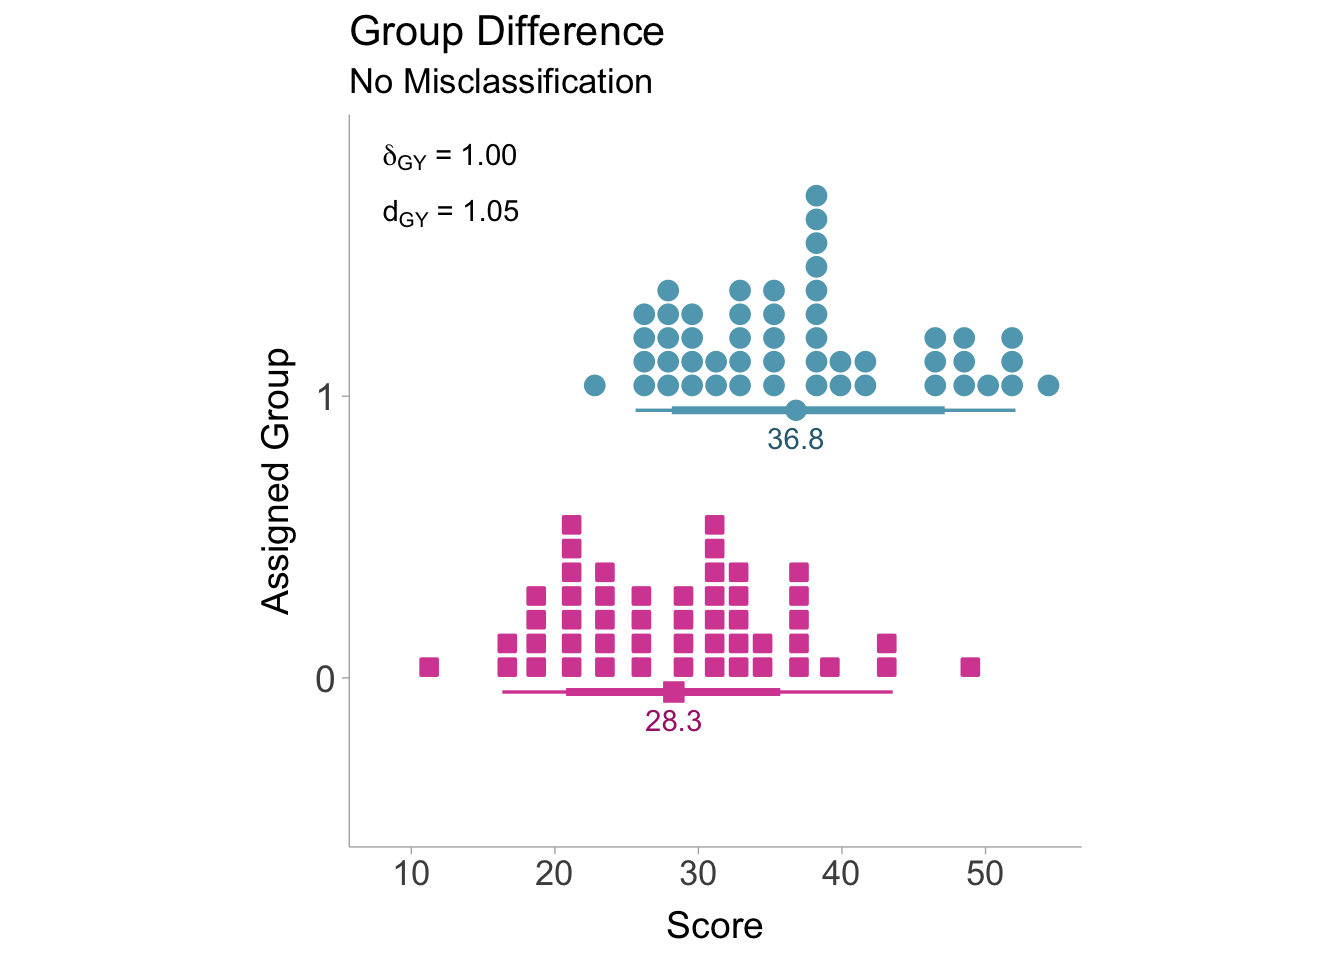
\includegraphics{chapters/05-misclassification/05-misclassification_files/figure-pdf/fig-no-mis-1.pdf}

}

\caption{\label{fig-no-mis}Distributions of scores without
misclassification. True mean difference and observed mean differ only
due to sampling error. Red squares denote actual group \(A\) members,
blue circles denote actual group \(B\) members.}

\end{figure}%

If some individuals are assigned to the incorrect group, then we will
see attenuation in the standardized mean difference as the means
converge. Figure~\ref{fig-mis} is showing what happens when the group
misclassification rate is 10\%. A group misclassification rate of 10\%
is equivalent to a classification reliability of \(r_{gg'}=.64\).

\begin{figure}[H]

\centering{

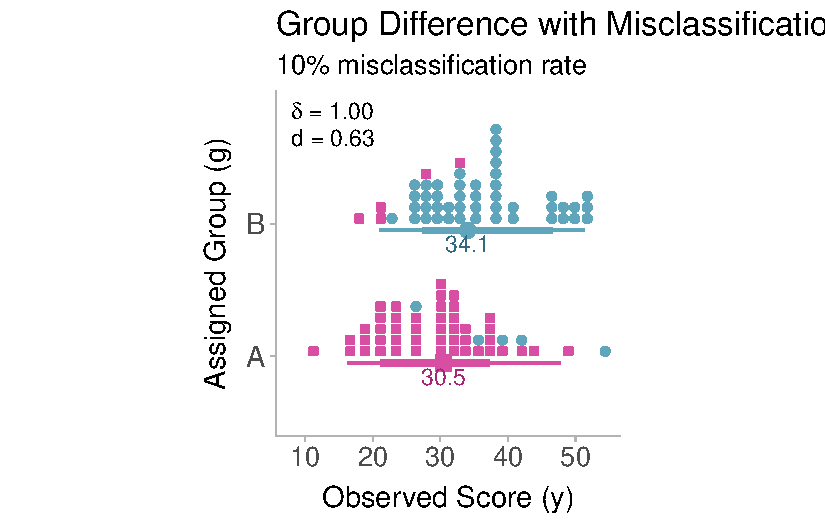
\includegraphics{chapters/05-misclassification/05-misclassification_files/figure-pdf/fig-mis-1.pdf}

}

\caption{\label{fig-mis}Distributions of scores with a 10\%
misclassification rate. Observed standardized mean differences are
biased toward the null (i.e., \(\delta\) = 0). Red squares denote actual
group \(A\) members, blue circles denote actual group \(B\) members.
Note that a few members of group \(A\) (red squares) are within assigned
group \(B\) and vice versa (indicative of misclassification).}

\end{figure}%

It is important to note that for many of the corrections converting the
standardized mean difference to a point-biserial correlation is often a
necessary step. However, once the corrected point-biserial correlation
is obtained, the correlation can then be converted back into a
standardized mean difference. To correct for bias induced by
misclassification we first need to convert the observed standardized
mean difference to a point-biserial correlation coefficient by using the
observed proportion of the sample that has been assigned to either group
\(A\) or group \(B\) (\(p_g\)). The group proportion \(p_g\) in the
following equations will only show up in the term \(p_g(1-p_g)\) so it
will not matter which group is used to calculate the proportion.
Converting \(d_{gY}\) to \(r_{gY}\):

\[
r_{gY} = \frac{d_{gY}}{\sqrt{\frac{1}{p_g(1-p_g)}-d_{gY}^2}}.
\]

We can then correct the point-biserial correlation for group
misclassification by dividing by the square root of the classification
reliability. Since we also want to correct for measurement error in the
continuous dependent variable, \(Y\), we can simultaneously apply the
correction for unreliability:

\[
r_{GU} = \frac{r_{gY}}{\sqrt{r_{gg'}}\sqrt{r_{YY'}}}.
\]

Now we can convert the corrected point-biserial correlation into a
corrected standardized mean difference (\(d_{GU}\)). When converting
back to a standardized mean difference, we need to use the true group
proportions, \(p_G\). Although if we are to assume equal
misclassification rates between groups, then the observed proportion can
be used \(p_g\):

\[
d_{GU} = \frac{r_{GU}}{\sqrt{p_G\left(1-p_G\right)\left(1-r_{GU}^2\right)}}.
\]

This process of converting, correcting, and then back-converting must
also be done for the standard error. To avoid redundancy, we can
incorporate each step into a single equation:

\[
\small{se(d_{GU}) = \frac {se(d_{gY})\times r_{GU}} {r_{gY}\sqrt{\left(1+d_{gY}^2p[1-p]\right)^2\left(d_{gY}^2+\frac{1}{p_g(1-p_g)}\right)p_G(1-p_G)(1-r_{GU}^2)^3}}.}
\]

\begin{tcolorbox}[enhanced jigsaw, opacityback=0, coltitle=black, toprule=.15mm, colframe=quarto-callout-note-color-frame, bottomtitle=1mm, rightrule=.15mm, colbacktitle=quarto-callout-note-color!10!white, left=2mm, bottomrule=.15mm, breakable, title={Applied Example in R}, colback=white, opacitybacktitle=0.6, titlerule=0mm, arc=.35mm, leftrule=.75mm, toptitle=1mm]

A researcher wants to compare the academic performance (measured by a
standardized test) of people with and without Major Depressive Disorder
(MDD). The researcher reports a classification reliability of
\(r_{gg'}=.80\) and a reliability of the standardized test as
\(r_{YY'}=.85\). The researcher than finds a standardized mean
difference of \(d_{gY}=.30\) favoring controls (i.e., controls had a
higher average on the test). Using the \texttt{correct\_d} function in
the \texttt{psychmeta} package, we can obtain an unbiased estimate of
the target standardized mean difference.

\begin{Shaded}
\begin{Highlighting}[]
\FunctionTok{library}\NormalTok{(psychmeta)}

\FunctionTok{correct\_d}\NormalTok{(}\AttributeTok{correction =} \StringTok{"meas"}\NormalTok{,}
          \AttributeTok{d =}\NormalTok{ .}\DecValTok{30}\NormalTok{,   }\CommentTok{\# observed standardized mean difference}
          \AttributeTok{ryy =}\NormalTok{ .}\DecValTok{85}\NormalTok{, }\CommentTok{\# reliability of dependent variable}
          \AttributeTok{rGg =} \FunctionTok{sqrt}\NormalTok{(.}\DecValTok{80}\NormalTok{), }\CommentTok{\# sqrt of classification reliability}
          \AttributeTok{n1 =} \DecValTok{100}\NormalTok{, }\CommentTok{\# sample size in controls}
          \AttributeTok{n2 =} \DecValTok{100}\NormalTok{) }\CommentTok{\# sample size in people with MDD}
\end{Highlighting}
\end{Shaded}

\begin{verbatim}
d Values Corrected for Measurement Error:
---------------------------------------------------------------------------------------
  value CI_LL_95 CI_UL_95   n n_effective
1 0.366   0.0238    0.726 200         133
\end{verbatim}

The corrected standardized mean difference is
\(d_{GU}=0.37\, [0.02,\, .73]\).

\end{tcolorbox}

\bookmarksetup{startatroot}

\chapter{Artificial Dichotomization}\label{sec-dichotomization}

\section{Introduction}\label{introduction-4}

Researchers occasionally split naturally continuous variables into two
discrete groups to increase interpretability or conduct specific
analyses (e.g., t-tests). However, artificially dichotomizing variables
introduces measurement error variance thus attenuating effect size
estimates Maxwell and Delaney (1993). The obvious solution to this
problem is to simply not dichotomize variables, however if only summary
data is available to us, then we may not have this luxury.
Dichotomization can also be practical in some instances. For example,
clinical disorder diagnoses such as generalized anxiety disorder, are
examples of dichotomization where individuals are separated into either
having the disorder or not even though individual differences in anxiety
exist as a continuum.

\section{Artificial Dichotomization Induced Measurement
Error}\label{artificial-dichotomization-induced-measurement-error}

Variables that are dichotomized contain measurement error. This can be
demonstrated by the simple fact that dichotomized scores are not
perfectly correlated with their underlying continuous scores. To
demonstrate this, we can draw a sample of scores and then split the data
into high and low scorers and then calculate the correlation coefficient
between the two (see Figure~\ref{fig-dich}).

\begin{figure}[H]

\centering{

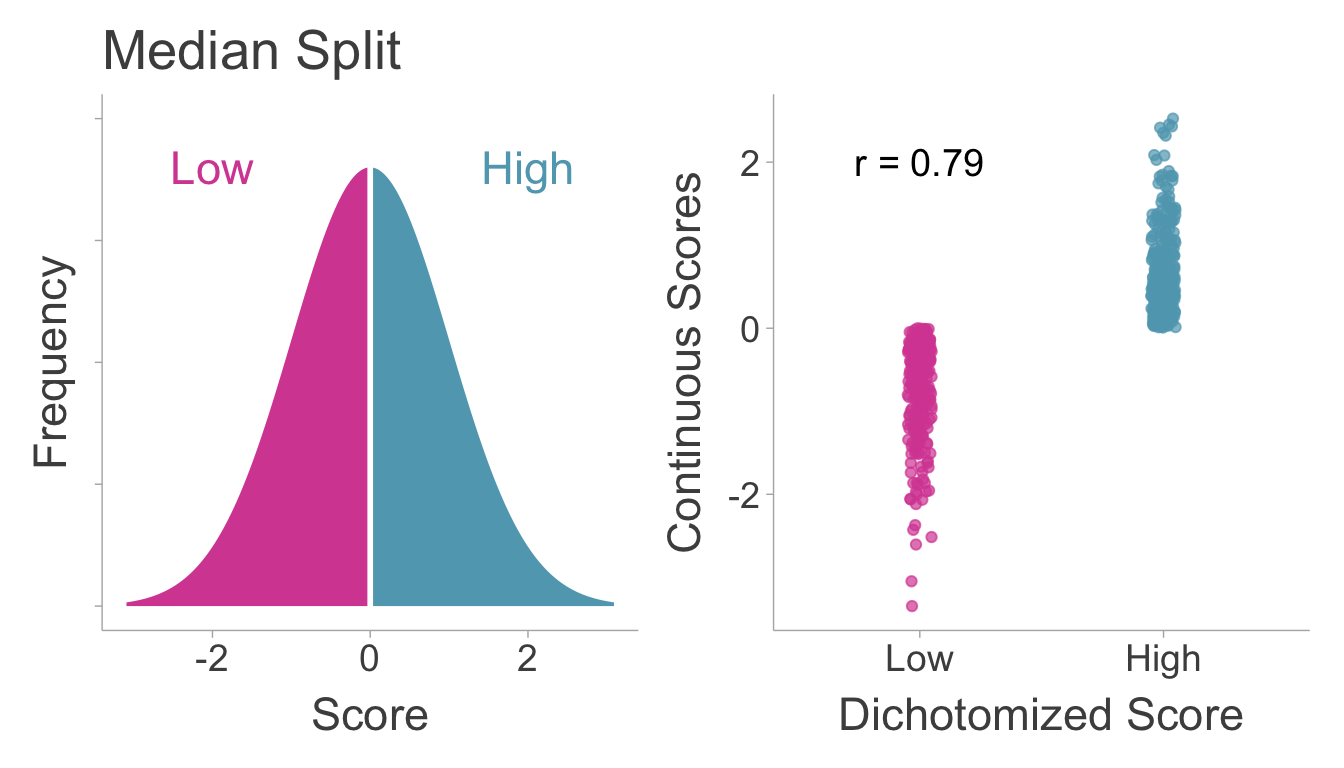
\includegraphics{chapters/06-artificial-dichotomization/06-artificial-dichotomization_files/figure-pdf/fig-dich-1.pdf}

}

\caption{\label{fig-dich}Visualizing the loss of precision when
artificially dichotomizing. Left panel shows a normally distributed
variable split (at the median/mean) into a high scoring group and a low
scoring group.}

\end{figure}%

Even with a perfectly reliable measure, dichotomization will introduce
measurement error. Dichotomization occurs when data is split into two
groups (low and high groups will be denoted as \(L\) and \(H\),
respectively) depending on whether they are above or below some
cut-point \(C_X\). We can define artificially dichotomized scores as,

\[
X_D= 
\begin{cases}
    H,& \text{if } X\geq C_X\\
    L,& \text{if } X<C_X
\end{cases}
\]

\section{Correcting Correlations for Artificial
Dichotomization}\label{correcting-correlations-for-artificial-dichotomization}

\subsection{Defining the Target
Quantity}\label{defining-the-target-quantity-3}

We want to obtain the population correlation between continuous scores
of the independent (\(X\)) and dependent variable (\(Y\)),
\(\rho_{XY}\).

There are two cases of dichotomization that may occur in a given study:
the \emph{univariate} case where only one variable (either \(X\)
\emph{or} \(Y\)) is dichotomized and the \emph{bivariate} case where
both variables are dichotomized. In either case, dichotomization will
have a biasing effect on the study correlation coefficient. The study
correlation on dichotomized data (using the bivariate case,
\(r_{X_D Y_D}\)) can be modeled as a function of the population
correlation on continuous scores (\(\rho_{XY}\); i.e., the target), an
artifact attenuation factor \(a\), and sampling error, \(e\),

\[
r_{X_DY_D} = a\rho_{XY}+e.
\]

An unbiased estimate of \(\rho_{XY}\) can be calculated by dividing the
study correlation by an estimate of the artifact attenuation factor,
\(a\),

\[
r_{XY} = \frac{r_{X_D Y_D}}{a}.
\]

\subsection{Artifact Correction for
Correlations}\label{sec-corr-artifacts}

Correlations can suffer from dichotomization in one variable (univariate
case) or both variables (bivariate case). This section will discuss the
procedure for obtaining an unbiased estimate of the correlation
coefficient for both cases. For a comparative visualization of a
correlation on with no dichotomization, univariate dichotomization, and
bivariate dichotomization, see Figure~\ref{fig-dich-cases}.

\begin{figure}[H]

\centering{

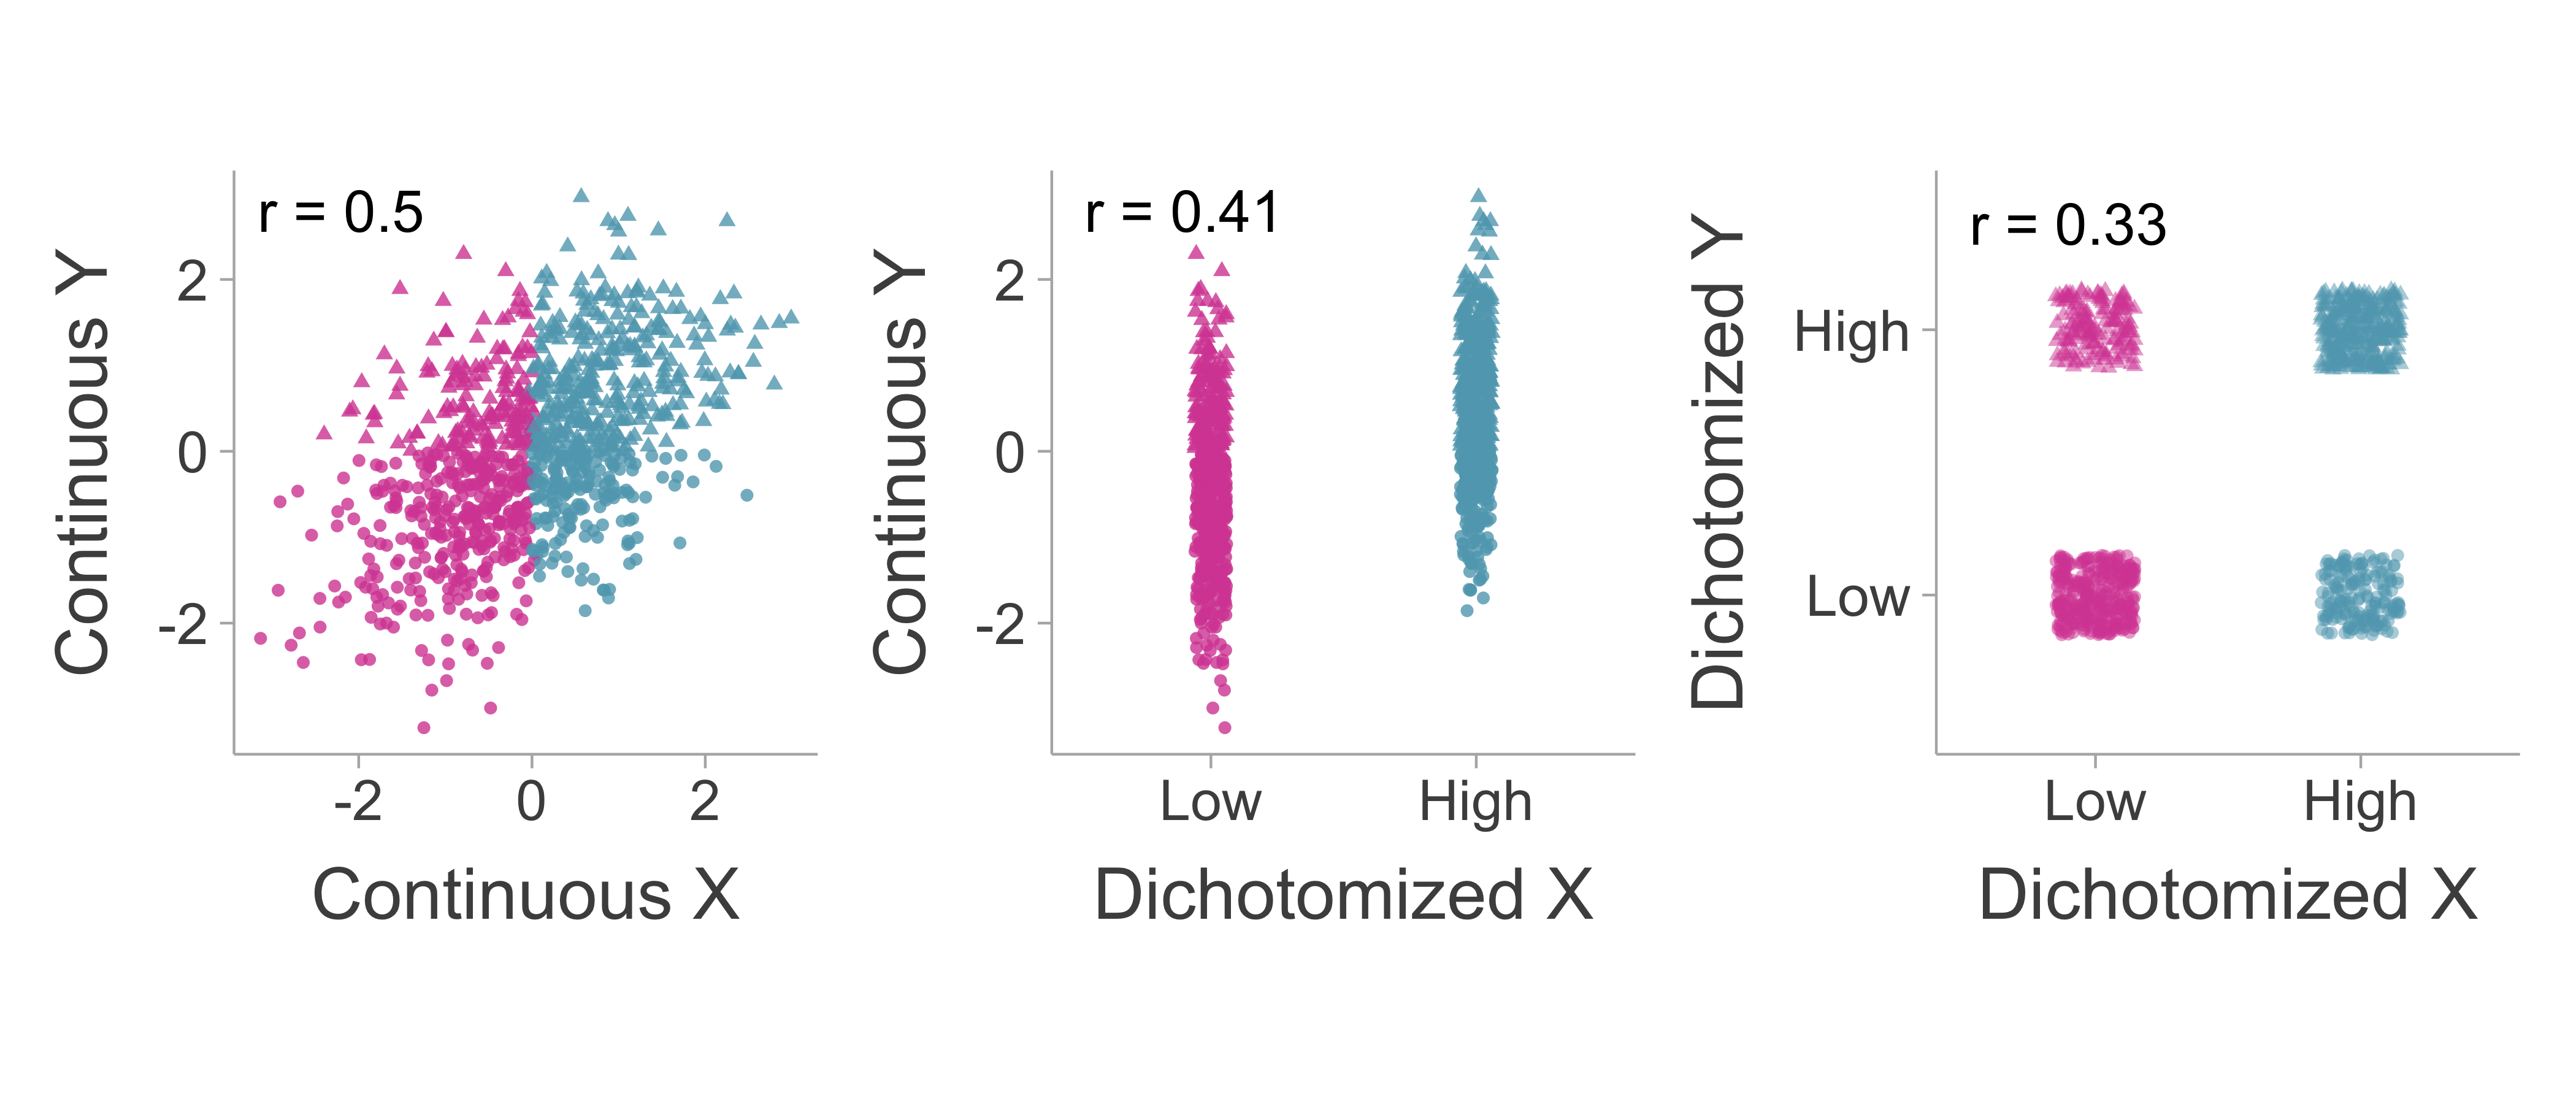
\includegraphics{chapters/06-artificial-dichotomization/06-artificial-dichotomization_files/figure-pdf/fig-dich-cases-1.pdf}

}

\caption{\label{fig-dich-cases}Scatter plots showing the correlation
under dichotomization. The first panel (left to right) shows the
correlation with no dichotomization (color and shapes of points denote
where the split in the dichotomized cases will occur). The middle panel
shows the univariate case where only the independent variable, \(X\), is
dichotomized. The last panel shows the bivariate case where both
independent (\(X\)) and dependent (\(Y\)) variables are dichotomized.}

\end{figure}%

\subsubsection*{The Univariate Case}\label{the-univariate-case}
\addcontentsline{toc}{subsubsection}{The Univariate Case}

In the simplest case of dichotomization, only one variable is
dichotomized and the other is left continuous. A Pearson correlation
computed between a dichotomous variable and a continuous variable is
known as \emph{point-biserial} correlation. However, if the variable is
naturally continuous, we can estimate the correlation of the underlying
continuous scores by computing a \emph{biserial} correlation. If all we
have access to is the dichotomized data, then we need to assume the
shape of the underlying distribution, in this case, the biserial
correlation assumes normality.

In the population, the study correlation \(\rho_{X_D Y}\) is biased by
some artifact biasing factor, \(a\),

\[
\rho_{X_D Y} = a\rho_{XY}.
\]

To estimate the attenuation factor \(a\), we must first figure out where
the split of the data occured. To do this, we must first calculate the
proportion of the sample in the assigned to the low or high scoring
group:

\[
p_X  := p(X_i \geq C_X) = \frac{ n_{\text{H}} }{n_{\text{H}} + n_{\text{L}}}
\]

or

\[
p_X := p(X_i < C_X) = \frac{ n_{\text{L}} }{n_{\text{H}} + n_{\text{L}}}.
\]

Where \(n\) indicates the sample size within the low, \(L\), and high,
\(H\), scoring groups.

\begin{tcolorbox}[enhanced jigsaw, opacityback=0, coltitle=black, toprule=.15mm, colframe=quarto-callout-tip-color-frame, bottomtitle=1mm, rightrule=.15mm, colbacktitle=quarto-callout-tip-color!10!white, left=2mm, bottomrule=.15mm, breakable, title={Note}, colback=white, opacitybacktitle=0.6, titlerule=0mm, arc=.35mm, leftrule=.75mm, toptitle=1mm]

It will not matter whether you calculate the proportion of the sample in
the high scoring group or the low scoring group for \(p_X\). Once you
decide on one, do not change it.

\end{tcolorbox}

We can use the quantile function (\(\phi^{-1}[\cdot]\), i.e., the
inverse of the cumulative density of the standard normal distribution)
to find where the split would have occured on a standard normal
distribution, \(s_X=\phi^{-1}[p_X]\). Using the location of the split on
the standard normal, we can compute the artifact attenuation factor
{[}an adaptation of equation 2, J. Hunter and Schmidt (1990){]},

\begin{equation}\phantomsection\label{eq-artifact-factor-dich}{
\hat{a} =\frac{\varphi\left(s_X\right)}{\sqrt{p_X(1-p_X)}}.
}\end{equation}

Where \(\varphi(\cdot)\) is the normal ordinate function (i.e.,
probability density function of a standard normal distribution).
Figure~\ref{fig-normal-density} visually demonstrates how each of these
relate to a standard normal distribution.

\begin{figure}[H]

\centering{

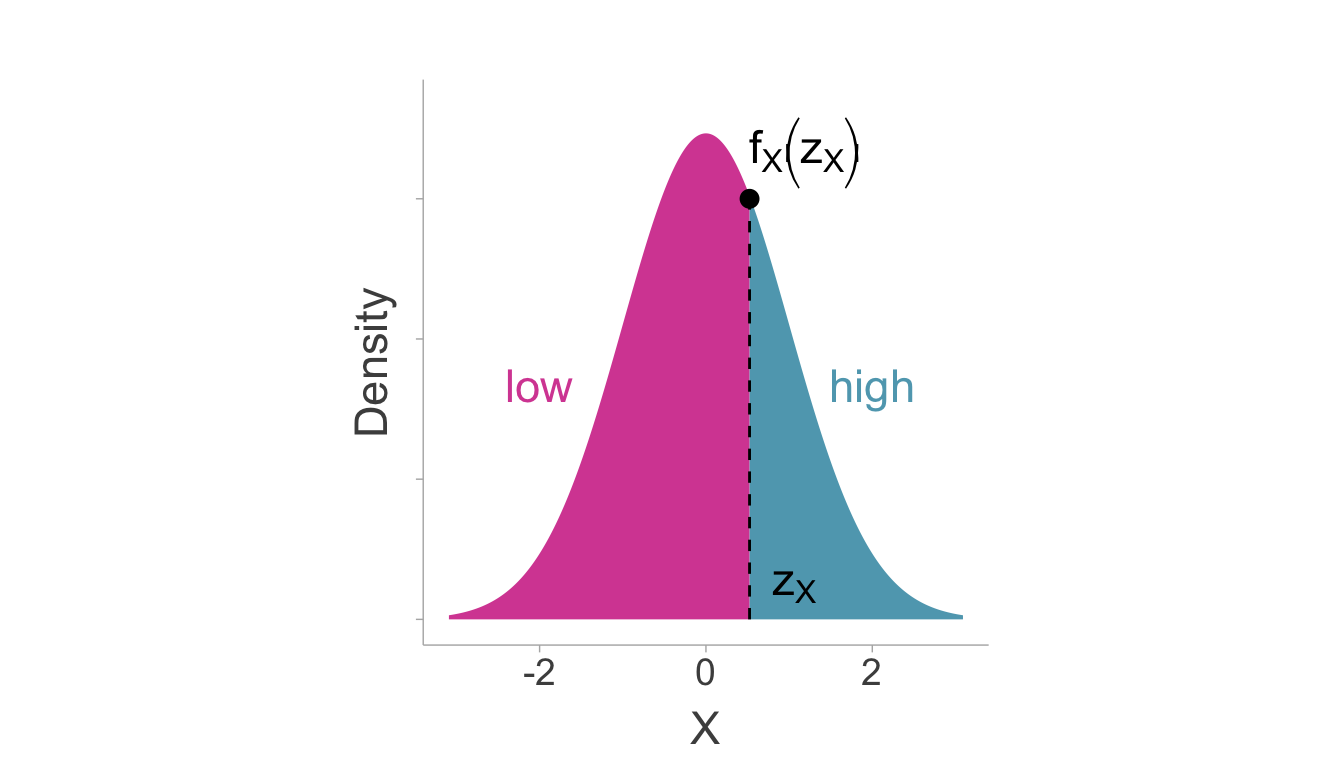
\includegraphics{chapters/06-artificial-dichotomization/06-artificial-dichotomization_files/figure-pdf/fig-normal-density-1.pdf}

}

\caption{\label{fig-normal-density}This figure shows a normal
distribution of scores split into a high scoring and low scoring group.
The cut-point of the standard normal distribution is computed with the
quantile function, \(\phi^{-1}[p_X]\). The ordinate of the normal
distribution at that cut-point is calculated with the normal ordinate
function, \(\varphi\left(\phi^{-1}[p_X]\right)\).}

\end{figure}%

In the case of a median split, where the cut-point would be placed at
zero of a standard normal (splitting the distribution in equal halves),
the attenuation factor would simplify to
\(\hat{a} =\frac{\varphi(0)}{\sqrt{.5(.5)}}\)
\(=\frac{2}{\sqrt{2\pi}}\).

We can correct the study correlation using the estimated artifact
factor, \(\hat{a}\), therefore the full correction equation is,

\begin{equation}\phantomsection\label{eq-dich-r}{
r_{XY} = \frac{r_{X_DY}}{\hat{a}} = \frac{r_{X_DY}}{\left[\frac{\varphi\left(s_X\right)}{\sqrt{p_X(1-p_X)}}\right]}.
}\end{equation}

\begin{tcolorbox}[enhanced jigsaw, opacityback=0, coltitle=black, toprule=.15mm, colframe=quarto-callout-tip-color-frame, bottomtitle=1mm, rightrule=.15mm, colbacktitle=quarto-callout-tip-color!10!white, left=2mm, bottomrule=.15mm, breakable, title={Converting to \(\boldsymbol{\mathsf{r_{X_{D}Y}}}\) from means and
standard deviations}, colback=white, opacitybacktitle=0.6, titlerule=0mm, arc=.35mm, leftrule=.75mm, toptitle=1mm]

It is common that studies do not report the correlation between
dichotomized and continuous scores, \(r_{X_DY}\) (i.e., the
point-biserial correlation), instead they may report the means and
standard deviations instead. To obtain the point-biserial correlation,
\(r_{X_D Y}\), we need the the mean of the high scoring group
(\(\overline{Y}_H\)), mean of the low scoring groups
(\(\overline{Y}_L\)), the standard deviation across all individuals
(\(S_Y\); not to be confused with the pooled/average standard deviation
within each group), and the sample sizes within each group (\(n_H\) and
\(n_L\)) to calculate \(r_{X_DY}\),

\[
r_{X_D Y} =\frac{\overline{Y}_H-\overline{Y}_L}{S_Y} \sqrt{p_X(1-p_X)}.
\]

If the standard deviations are reported only for within the high and low
groups, you can estimate the total standard deviation with the following
formula,

\[
S_X = \sqrt{\frac{n_HS_{X_H} + n_L S_{X_L}}{n_H + n_L} +\frac{n_Hn_L}{n_H + n_L}(\overline{X}_H - \overline{X}_L)^2}.
\]

\end{tcolorbox}

J. Hunter and Schmidt (1990) suggested that one should correct the
standard error by dividing the uncorrected standard error by the
artifact attenuation factor (see equation 6, J. Hunter and Schmidt
1990). However simulations have found that this computation does not
work as well as Soper's exact method (Soper 1914; Jacobs and Viechtbauer
2017). Therefore the standard error of the corrected (biserial)
correlation can be estimated with the following formula (equation 12,
Jacobs and Viechtbauer 2017),

\[
\small{se(r_{XY}) = \sqrt{\frac{1}{n-1} \left(r_{XY}^4+r_{XY}^2\left(\frac{p_X(1-p_X)s_X^2}{\varphi\left(s_X\right)^2} + \frac{2p_X - 1}{\varphi\left(s_X\right)} -\frac{5}{2}\right)+\frac{p_X(1-p_X)}{\varphi\left(s_X\right)^2}\right)}}.
\]

Soper (1914) also developed an approximation of the above formula,

\[
se(r_{XY}) \approx \sqrt{\frac{1}{n-1}} \left(\frac{\sqrt{p_X(1-p_X)}}{\varphi\left(s_X\right)}-r_{XY}^2\right).
\]

\begin{tcolorbox}[enhanced jigsaw, opacityback=0, coltitle=black, toprule=.15mm, colframe=quarto-callout-note-color-frame, bottomtitle=1mm, rightrule=.15mm, colbacktitle=quarto-callout-note-color!10!white, left=2mm, bottomrule=.15mm, breakable, title={Applied Example in R}, colback=white, opacitybacktitle=0.6, titlerule=0mm, arc=.35mm, leftrule=.75mm, toptitle=1mm]

Let's say we want to assess the relationship between a sales person's
score on a job knowledge test and their job performance estimated as the
number of sales made per week. However the researchers of the study
chose to dichotomize sales people into high sales performers and low
sales performers by splitting the sample into two equally sized groups.
They then reported the means and standard deviations of job knowledge
test scores of both groups:

\begin{enumerate}
\def\labelenumi{\arabic{enumi}.}
\tightlist
\item
  Low sales performers: Mean = 22 (SD = 4, n = 50)
\item
  High sales performers: Mean = 24 (SD = 4, n = 50)
\end{enumerate}

To calculate the corrected correlation we can use \texttt{escalc()}
function from the \texttt{metafor} package (Viechtbauer 2010). Using the
argument \texttt{measure=\textquotesingle{}RBIS\textquotesingle{}} will
return the biserial correlation coefficient which is equivalent to the
corrected correlation.

\begin{Shaded}
\begin{Highlighting}[]
\FunctionTok{library}\NormalTok{(metafor)}

\FunctionTok{escalc}\NormalTok{(}\AttributeTok{measure =} \StringTok{\textquotesingle{}RBIS\textquotesingle{}}\NormalTok{,}
       \AttributeTok{m1i =} \DecValTok{24}\NormalTok{, }\CommentTok{\# High performer mean }
       \AttributeTok{m2i =} \DecValTok{22}\NormalTok{, }\CommentTok{\# Low performer mean}
       \AttributeTok{sd1i =} \DecValTok{4}\NormalTok{, }\CommentTok{\# High performer SD}
       \AttributeTok{sd2i =} \DecValTok{4}\NormalTok{, }\CommentTok{\# Low performer SD}
       \AttributeTok{n1i =} \DecValTok{50}\NormalTok{, }\CommentTok{\# High performer sample size}
       \AttributeTok{n2i =} \DecValTok{50}\NormalTok{, }\CommentTok{\# Low performer sample size}
       \AttributeTok{var.names =} \FunctionTok{c}\NormalTok{(}\StringTok{\textquotesingle{}rXY\textquotesingle{}}\NormalTok{,}\StringTok{\textquotesingle{}se.2\textquotesingle{}}\NormalTok{),}
       \AttributeTok{digits =} \DecValTok{3}\NormalTok{)}
\end{Highlighting}
\end{Shaded}

\begin{verbatim}

    rXY  se.2 
1 0.307 0.014 
\end{verbatim}

Therefore the estimated correlation on continuous scores is
\(r_{XY}=.31\).

If the study reported a Pearson correlation (point-biserial) between the
dichotomized variable and the continuous variable of \(r_{X_D Y}=.245\),
then

\begin{Shaded}
\begin{Highlighting}[]
\FunctionTok{library}\NormalTok{(psychmeta)}

\FunctionTok{correct\_r\_dich}\NormalTok{(}\AttributeTok{r =}\NormalTok{ .}\DecValTok{245}\NormalTok{, }\CommentTok{\# study point{-}biserial correlation}
               \AttributeTok{px =}\NormalTok{ .}\DecValTok{50}\NormalTok{, }\CommentTok{\# proportion of sample in low or high group}
               \AttributeTok{n =} \DecValTok{100}\NormalTok{) }\CommentTok{\# total sample size}
\end{Highlighting}
\end{Shaded}

\begin{verbatim}
  r_corrected var_e_corrected    n_adj
1    0.307062      0.01401901 59.51455
\end{verbatim}

The corrected correlation for continuous scores is equal to the
calculation using the means and standard deviations. Note that the
estimated sampling variance of the corrected correlation, \texttt{se.2}
(in the \texttt{psychmeta} example) and \texttt{var\_e\_corrected} (in
the \texttt{metafor} example), are both equal to the squared corrected
standard error (\(se(r_{XY})^2\)).

\end{tcolorbox}

\subsubsection*{The Bivariate Case}\label{the-bivariate-case}
\addcontentsline{toc}{subsubsection}{The Bivariate Case}

In some cases, both independent and dependent variables are
dichotomized. A Pearson correlation calculated on these two dichotomized
(binary) variables would be equal to the phi coefficient (or also known
as Matthew's correlation coefficient) and we can denote it with our
notation for dichotomized variables, \(\rho_{X_D X_D}\). Dichotomized
data can be structured in a contingency table (see
Table~\ref{tbl-biv-dich}).

\begin{longtable}[]{@{}ccc@{}}
\caption{Contingency table.}\label{tbl-biv-dich}\tabularnewline
\toprule\noalign{}
\endfirsthead
\endhead
\bottomrule\noalign{}
\endlastfoot
& \(X_D=\text{Low}\) & \(X_D=\text{High}\) \\
\(Y_D=\text{Low}\) & \(n_{LL}\) & \(n_{HL}\) \\
\(Y_D=\text{High}\) & \(n_{LH}\) & \(n_{HH}\) \\
\end{longtable}

Figure~\ref{fig-biv-dich} illustrates how this contingency table relates
to an underlying continuous bivariate normal distribution.

\begin{figure}[H]

\centering{

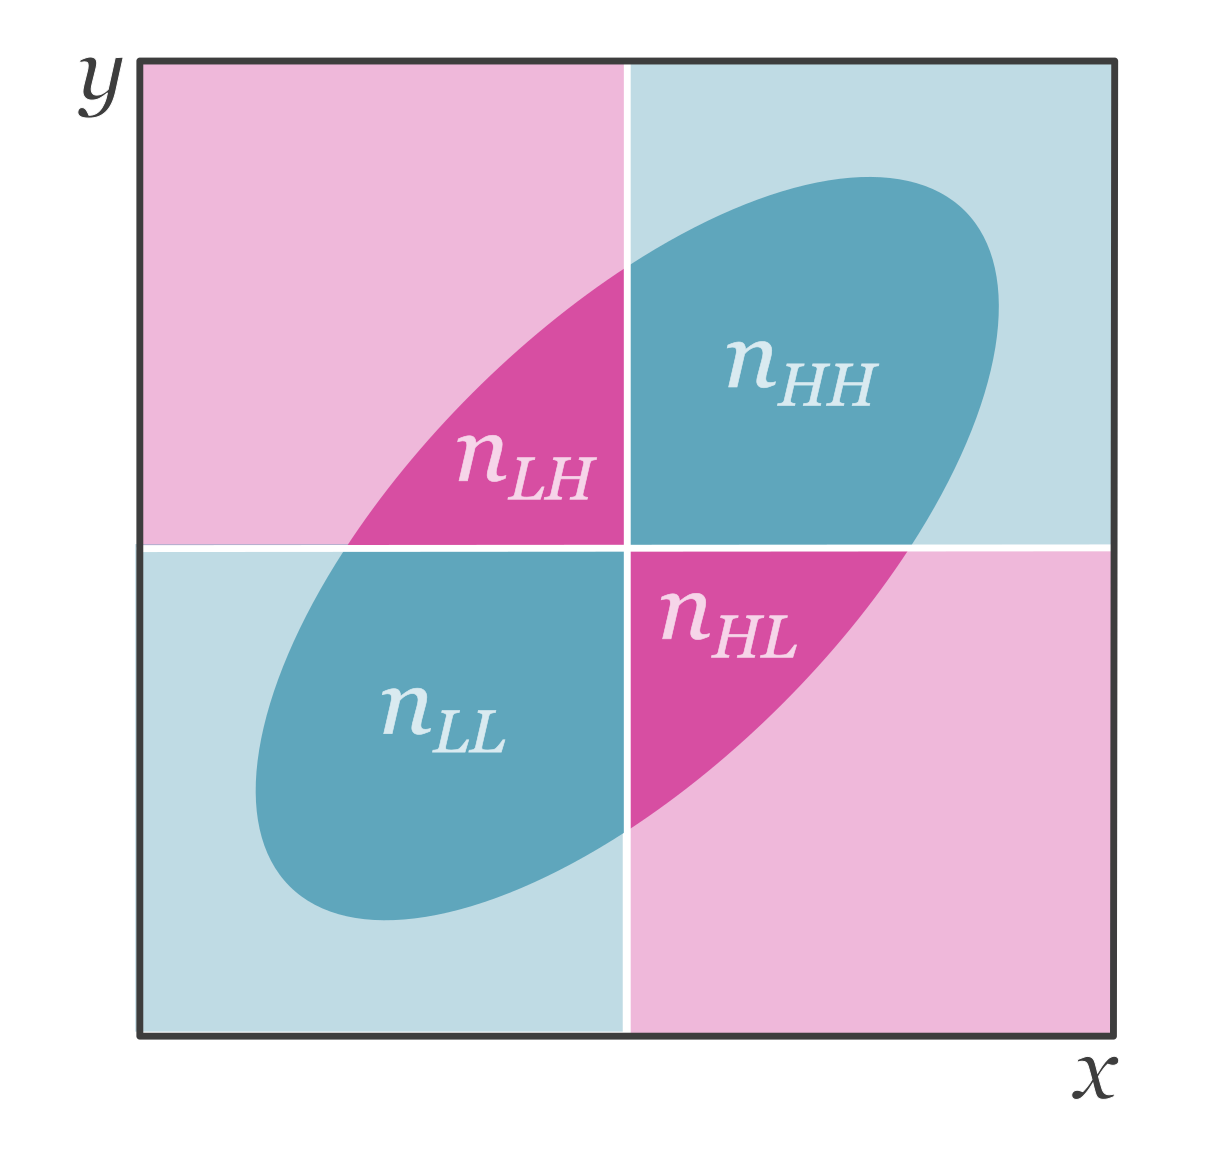
\includegraphics[width=0.6\textwidth,height=\textheight]{chapters/06-artificial-dichotomization/figure/diagram-dich.png}

}

\caption{\label{fig-biv-dich}The ellipse indicates the bivariate normal
distribution of \(X\) and \(Y\) with a strong positive correlation. If
\(X\) and \(Y\) are positively correlated then we should more
individuals populating the high-high and low-low cells rather than the
high-low and low-high cells which can be seen by the area of the ellipse
located in each quadrant.}

\end{figure}%

The corrected correlation coefficient for two dichotomized variables is
commonly referred to as the tetrachoric correlation coefficient. The
tetrachoric correlation estimates the correlation on continuous scores
assuming a bivariate normal distribution.

One of the difficulties of computing a dichotomization corrected
(tetrachoric) correlation (\(r_{XY}\)) is that the relationship between
binary variables are reported in different ways across studies, we will
describe how to obtain a dichtomization corrected correlation in four
different cases:

\begin{enumerate}
\def\labelenumi{\arabic{enumi}.}
\tightlist
\item
  The full contingency table is provided, including the sample sizes for
  each cell.
\item
  The odds ratio is reported as well as the marginal proportions
  (proportions in low and high groups for each variable).
\item
  The Phi coefficient is reported.
\end{enumerate}

\paragraph*{Case 1: Full contingency table is
reported}\label{case-1-full-contingency-table-is-reported}
\addcontentsline{toc}{paragraph}{Case 1: Full contingency table is
reported}

If the full contingency table is reported, then the tetrachoric
correlation can be calculated directly. Due to the complexity of the
calculation, we will use R.

The \texttt{escalc()} function in the \texttt{metafor} package
(Viechtbauer 2010) can take on values from a contingency table and
compute a tetrachoric correlation using the
\texttt{measure=\textquotesingle{}RTET\textquotesingle{}} argument. The
function uses the method described by Kirk (1973).

\begin{Shaded}
\begin{Highlighting}[]
\CommentTok{\# Example Contingency Table}
\CommentTok{\#    XL   XH}
\CommentTok{\# YL 43   23}
\CommentTok{\# YH 27   38  }

\FunctionTok{library}\NormalTok{(metafor)}

\FunctionTok{escalc}\NormalTok{(}\AttributeTok{measure =} \StringTok{\textquotesingle{}RTET\textquotesingle{}}\NormalTok{,}
       \AttributeTok{ai =} \DecValTok{43}\NormalTok{,}
       \AttributeTok{bi =} \DecValTok{23}\NormalTok{,}
       \AttributeTok{ci =} \DecValTok{27}\NormalTok{,}
       \AttributeTok{di =} \DecValTok{38}\NormalTok{,}
       \AttributeTok{var.names =} \FunctionTok{c}\NormalTok{(}\StringTok{\textquotesingle{}rXY\textquotesingle{}}\NormalTok{,}\StringTok{\textquotesingle{}se.2\textquotesingle{}}\NormalTok{))}
\end{Highlighting}
\end{Shaded}

\begin{verbatim}

     rXY   se.2 
1 0.3637 0.0155 
\end{verbatim}

The results show a dichotomization corrected correlation of
\(r_{XY} = .36\) and an estimated sampling variance of \(se_c^2=.016\).

\paragraph*{Case 2: odds ratio is
reported}\label{case-2-odds-ratio-is-reported}
\addcontentsline{toc}{paragraph}{Case 2: odds ratio is reported}

If the odds ratio is all that is available, then we can use the
tetrachoric correlation approximation described by Bonett and Price
(2005). Using the estimated odds ratio
(\(OR=(n_{HH}n_{LL})/(n_{HL}n_{LH})\)) and the marginal proportions
(\(p_X\) and \(p_Y\); for this case, both proportions should be with
respect to the high scoring group) we can approximate the
dichotomization corrected (tetrachoric) correlation (see equation 4,
Bonett and Price 2005),

\[
r_{XY} \approx \cos\left( \frac{\pi}{1+OR^\Omega}\right)
\] Where \(\Omega\) is

\[
\Omega = 1 - \frac{\left|p_X -p_Y\right|}{5} - \left[\frac{1}{2}-\min(p_X,p_Y)\right]^2.
\]

Note that \(\min(p_X,p_Y)\) is the smallest marginal proportion. The
standard error of the estimated correlation can be computed with the
following formula {[}see equation 9, Bonett and Price (2005); note this
equation is slightly changed in order to account for the fact that we
only have access to the marginal sample sizes and proportions{]}

\[
\small{se(r_{XY}) =  \frac{\pi\times \Omega\times OR^\Omega\times\sin\left(\frac{\pi}{1+OR^\Omega}\right)}{\left(1+OR^\Omega\right)^2}\times\sqrt{\frac{4}{n}}}
\]

Where \(n\) is the total sample size. Using base R, we can convert the
odds ratio to a tetrachoric correlation.

\begin{Shaded}
\begin{Highlighting}[]
\NormalTok{pX }\OtherTok{\textless{}{-}}\NormalTok{ .}\DecValTok{4} \CommentTok{\# proportion of individuals in high group in XD}
\NormalTok{pY }\OtherTok{\textless{}{-}}\NormalTok{ .}\DecValTok{5} \CommentTok{\# proportion of individuals in high group in YD}
\NormalTok{n }\OtherTok{\textless{}{-}} \DecValTok{150} \CommentTok{\# total sample size}
\NormalTok{OR }\OtherTok{\textless{}{-}} \FloatTok{1.43} \CommentTok{\# odds ratio}
\NormalTok{omega }\OtherTok{\textless{}{-}} \DecValTok{1} \SpecialCharTok{{-}} \FunctionTok{abs}\NormalTok{(pX}\SpecialCharTok{{-}}\NormalTok{pY) }\SpecialCharTok{/} \DecValTok{5} \SpecialCharTok{{-}}\NormalTok{ (}\DecValTok{1}\SpecialCharTok{/}\DecValTok{2} \SpecialCharTok{{-}} \FunctionTok{min}\NormalTok{(}\FunctionTok{c}\NormalTok{(pX,pY)))}\SpecialCharTok{\^{}}\DecValTok{2}

\CommentTok{\# calculate corrected correlation}
\NormalTok{rXY }\OtherTok{\textless{}{-}} \FunctionTok{cos}\NormalTok{(pi}\SpecialCharTok{/}\NormalTok{(}\DecValTok{1}\SpecialCharTok{+}\NormalTok{OR}\SpecialCharTok{\^{}}\NormalTok{omega))}

\CommentTok{\# calculate standard error}
\NormalTok{se }\OtherTok{\textless{}{-}}\NormalTok{ pi}\SpecialCharTok{*}\NormalTok{omega}\SpecialCharTok{*}\NormalTok{OR}\SpecialCharTok{\^{}}\NormalTok{omega}\SpecialCharTok{*}\FunctionTok{sin}\NormalTok{(pi}\SpecialCharTok{/}\NormalTok{(}\DecValTok{1}\SpecialCharTok{+}\NormalTok{OR}\SpecialCharTok{\^{}}\NormalTok{omega)) }\SpecialCharTok{/}\NormalTok{ (}\DecValTok{1}\SpecialCharTok{+}\NormalTok{OR}\SpecialCharTok{\^{}}\NormalTok{omega)}\SpecialCharTok{\^{}}\DecValTok{2} \SpecialCharTok{*} \FunctionTok{sqrt}\NormalTok{(}\DecValTok{4}\SpecialCharTok{/}\NormalTok{n)}

\FunctionTok{cbind}\NormalTok{(rXY, se)}
\end{Highlighting}
\end{Shaded}

\begin{verbatim}
           rXY      se
[1,] 0.2665276 0.11637
\end{verbatim}

\paragraph*{Case 3: Correlation between dichotomized
variables}\label{case-3-correlation-between-dichotomized-variables}
\addcontentsline{toc}{paragraph}{Case 3: Correlation between
dichotomized variables}

A Pearson correlation coefficient calculated between two binary
variables is most commonly referred to as a Phi coefficient or Matthew's
correlation coefficient. However, the Phi coefficient underestimates the
correlation on the underlying continuous scores (assuming bivariate
normality). Therefore we can approximate the correlation on continuous
scores by using a similar correction to the univariate case. We can
define an artifact attenuation factor that is similar to
Equation~\ref{eq-artifact-factor-dich}, but with the added attenuation
of \(Y_D\),

\[
\hat{a} =\left[\frac{\varphi\left(\phi^{-1}[p_X]\right)}{\sqrt{p_X(1-p_X)}}\right]\times\left[\frac{\varphi\left(\phi^{-1}[p_Y]\right)}{\sqrt{p_Y(1-p_Y)}}\right].
\]

Therefore we can correct \(r_{X_DY_D}\) for dichotomization in both
variables by dividing by the attenuation factor, \[
r_{XY} = \frac{r_{X_DY_D}}{\hat{a}}=\frac{r_{X_DY_D}}{\left[\frac{\varphi\left(\phi^{-1}[p_X]\right)}{\sqrt{p_X(1-p_X)}}\right]\times\left[\frac{\varphi\left(\phi^{-1}[p_Y]\right)}{\sqrt{p_Y(1-p_Y)}}\right]}
\] This correction is only an approximation, however it performs fairly
well when the correlation is below .8 (J. Hunter and Schmidt 1990). The
standard error of the corrected correlation can be calculated similarly
(adaptation of equation 9, J. Hunter and Schmidt 1990),

\[
se(r_{XY})=\frac{se(r_{X_DY_D})}{\left[\frac{\varphi\left(\phi^{-1}[p_X]\right)}{\sqrt{p_X(1-p_X)}}\right]\times\left[\frac{\varphi\left(\phi^{-1}[p_Y]\right)}{\sqrt{p_Y(1-p_Y)}}\right]}
\]

Using the \texttt{correct\_r\_dich()} function in the \texttt{psychmeta}
package (Dahlke and Wiernik 2019), we can correct the observed study
correlation for dichotomization.

\begin{Shaded}
\begin{Highlighting}[]
\FunctionTok{library}\NormalTok{(psychmeta)}

\FunctionTok{correct\_r\_dich}\NormalTok{(}\AttributeTok{r =}\NormalTok{ .}\DecValTok{20}\NormalTok{,  }\CommentTok{\# observed study correlation}
               \AttributeTok{px =}\NormalTok{ .}\DecValTok{50}\NormalTok{, }\CommentTok{\# proportion of sample in high group of XD}
               \AttributeTok{py =}\NormalTok{ .}\DecValTok{50}\NormalTok{, }\CommentTok{\# proportion of sample in high group of YD}
               \AttributeTok{n =} \DecValTok{100}\NormalTok{)  }\CommentTok{\# sample size}
\end{Highlighting}
\end{Shaded}

\begin{verbatim}
  r_corrected var_e_corrected    n_adj
1   0.3141593      0.02296926 36.36678
\end{verbatim}

The output shows the corrected correlation to be \(r_{XY}=.31\) and it's
estimated sampling variance \(se_c^2=.023\).

\section{Correcting Standardized Mean Differences for Artificial
Dichotomization}\label{correcting-standardized-mean-differences-for-artificial-dichotomization}

\subsection{Defining our Target
Quantity}\label{defining-our-target-quantity-1}

The target quantity is the standardized mean difference between groups
of a naturally continuous variable. Our target can thus be defined as
the population standardized mean difference between groups \(A\) and
\(B\) on continuous scores of the dependent variable, \(\delta_{gY}\).
For a given study the dichotomized standardized mean difference
(\(d_{gY_D}\)) can be defined as

\[
d_{gY_D} = a\delta_{gY} + e
\]

Therefore to obtain an unbiased estimate of the target quantity, we can
correct the observed study standardized mean difference by dividing by
the attenuation factor,

\[
d_{gY} = \frac{d_{gY_D}}{\hat{a}}
\]

\subsection{Artifact Correction for Standardized Mean
Differences}\label{sec-corr-smd}

The simplest way to correct for dichotomization in a standardized mean
difference is to first convert the observed \(d\) value of the
dichotomized dependent variable to a correlation coefficient. When
converting to a correlation coefficient, it's important to note the
binary nature of both variables, leading us to estimate the phi
coefficient rather than the point-biserial correlation that we would be
estimating if the dependent variable was continuous. To calculate the
phi coefficient from a \(d\) value we can use the proportion of group
membership in group \(A\) or group \(B\) (\(p_g\); it does not matter
which one is chosen, as long as it is consistent for every instance of
\(p_g\)),

\[
r_{gY_D} = \frac{d_{gY_D}}{\sqrt{d_{gY_D}^2+\frac{1}{p(1-p)}}}
\]

We can then correct the correlation similar to how we did in
Section~\ref{sec-corr-artifacts},

\[
r_{gY} = \frac{r_{gY_D}}{\left[\frac{\varphi\left(\phi^{-1}[p_Y]\right)}{\sqrt{p_Y(1-p_Y)}}\right]}.
\]

Then we can convert the corrected correlation back into a standardized
mean difference,

\[
d_{gY} = \frac{r_{gY}}{\sqrt{p_g\left(1-p_g\right)\left(1-r_{gY}^2\right)}}.
\]

Where \(d_{gY}\) is our corrected correlation (i.e., the estimated
correlation on continuous variables). The observed sampling variance
must also be corrected using the same three step procedure. For
simplicity, we will consolidate this into one formula,

\[
se(d_{gY}) = \frac {se(d_{gY_D}) \times r_{XY}} {r_{x_DY_D}\sqrt{\left(1+d_{gY_D}^2p_g[1-p_g]\right)^3(1-r_{gY}^2)^3}}.
\]

\subsubsection*{Obtaining Standardized Mean Difference from Odds
Ratio}\label{obtaining-standardized-mean-difference-from-odds-ratio}
\addcontentsline{toc}{subsubsection}{Obtaining Standardized Mean
Difference from Odds Ratio}

In most cases, difference in dichotomized outcomes between two groups is
unlikely to be reported as a standardized mean difference, instead it
will be more commonly reported as an odds ratio (\(OR\)). The odds ratio
is asymmetric about 1 (i.e., the null), but we can make it symmetric by
log transforming it (\(\log(OR)\)). The standard error of the log odds
ratio can be defined as,

\[
se(\log(OR)) = \sqrt{\frac{1}{n_{AH}} + \frac{1}{n_{AL}} + \frac{1}{n_{BH}} + \frac{1}{n_{BL}}}
\]

The equation above requires the full contingency table to compute. From
there we can use the cox-logit method to convert the odds ratio to a
standardized mean difference (Cox 1989; Haddock, Rindskopf, and Shadish
1998). Them method is quite simple as it just divides the log odds ratio
by 1.65,

\begin{equation}\phantomsection\label{eq-or-d}{
d_{gY} = \frac{\log(OR)}{1.65}
}\end{equation}

and the corresponding sampling variance of the \(d\) value is,

\[
se(d_{gY}) = \frac{se(\log(OR))}{1.65}.
\]

\begin{tcolorbox}[enhanced jigsaw, opacityback=0, coltitle=black, toprule=.15mm, colframe=quarto-callout-note-color-frame, bottomtitle=1mm, rightrule=.15mm, colbacktitle=quarto-callout-note-color!10!white, left=2mm, bottomrule=.15mm, breakable, title={Applied Example in R}, colback=white, opacitybacktitle=0.6, titlerule=0mm, arc=.35mm, leftrule=.75mm, toptitle=1mm]

Let's consider a hypothetical scenario where we want to examine the
relationship between caffeine consumption and the occurrence of heart
palpitations in a population. Our target quantity in this case is the
standardized mean difference of coffee consuption between people with
and without heart palpitations. The variable of interest, caffeine
consumption, is continuous (measured in milligrams per day). However,
the researcher decides to dichotomize this variable into two groups:
``High Caffeine Consumers'' and ``Low Caffeine Consumers.''

Suppose we have a sample of 500 individuals, and we dichotomize their
caffeine consumption into ``High Caffeine Consumers'' (more than 250mg
per day) and ``Low Caffeine Consumers'' (less than or equal to 250mg per
day). We also observe the occurrence of heart palpitations in these
individuals.

\begin{longtable}[]{@{}lcc@{}}
\toprule\noalign{}
& Heart Palpitations: Yes & Heart Palpitations: No \\
\midrule\noalign{}
\endhead
\bottomrule\noalign{}
\endlastfoot
High Consumers & 60 & 140 \\
Low Consumers & 20 & 280 \\
\end{longtable}

We can calculate the dichotomization corrected standardized mean
difference by calculating the log odds ratio with \texttt{escalc()}
function and then applying Equation~\ref{eq-or-d} to estimate
\(d_{gY}\).

\begin{Shaded}
\begin{Highlighting}[]
\CommentTok{\# calculate log{-}odds ratio}
\NormalTok{OR }\OtherTok{\textless{}{-}} \FunctionTok{escalc}\NormalTok{(}\AttributeTok{measure =} \StringTok{\textquotesingle{}OR\textquotesingle{}}\NormalTok{,}
             \AttributeTok{ai =} \DecValTok{60}\NormalTok{,}
             \AttributeTok{bi =} \DecValTok{140}\NormalTok{,}
             \AttributeTok{ci =} \DecValTok{20}\NormalTok{,}
             \AttributeTok{di =} \DecValTok{280}\NormalTok{,}
             \AttributeTok{var.names =} \FunctionTok{c}\NormalTok{(}\StringTok{\textquotesingle{}logOR\textquotesingle{}}\NormalTok{,}\StringTok{\textquotesingle{}se.2\textquotesingle{}}\NormalTok{))  }

\CommentTok{\# convert to standardized mean difference}
\NormalTok{dgY }\OtherTok{\textless{}{-}}\NormalTok{ OR}\SpecialCharTok{$}\NormalTok{logOR }\SpecialCharTok{/} \FloatTok{1.65}
\NormalTok{se }\OtherTok{\textless{}{-}} \FunctionTok{sqrt}\NormalTok{(OR}\SpecialCharTok{$}\NormalTok{se}\FloatTok{.2}\NormalTok{) }\SpecialCharTok{/} \FloatTok{1.65}

\CommentTok{\# print results}
\FunctionTok{cbind}\NormalTok{(dgY,se)}
\end{Highlighting}
\end{Shaded}

\begin{verbatim}
          dgY        se
[1,] 1.085915 0.1685905
\end{verbatim}

We can see that the standardized mean difference is estimated to be
\(d_{gY}=1.09\) and the corrected standard error is \(se_c=.169\)

\end{tcolorbox}

\bookmarksetup{startatroot}

\chapter{Scale Coarseness}\label{scale-coarseness}

\section{Introduction}\label{introduction-5}

Scale coarseness describes a situation where a variable that is
naturally continuous (e.g., happiness) is binned into discrete values
(e.g., happiness measured on a scale of 1-10). This situation is quite
common in the social and psychological sciences where Likert items or
dichotomous yes/no responses are aggregated to form a coarse total score
for a naturally continuous construct. When coarseness is present,
measurement error is introduced into the observed scores and those
scores lose information. Unlike dichotomization, coarseness is an
artifact that occurs due to the design of the study rather than during
the analysis phase (Aguinis, Pierce, and Culpepper 2009). Particularly,
dichotomization occurs after scores are obtained (e.g., splitting a
group into high scorers and low scorers), whereas coarseness occurs as
an artifact of the measurement procedure itself. The primary issue with
coarseness is that it limits the set of possible values a score can be
which introduces error when the variable is naturally continuous. This
can be visualized by correlating coarse scores with their underlying
continuous scores (see Figure~\ref{fig-coarse-self}). You will notice
that the correlation between coarse and continuous scores is not
perfect, indicating that the coarse scores do not perfectly capture the
underlying continuous scores.

\begin{figure}[H]

\centering{

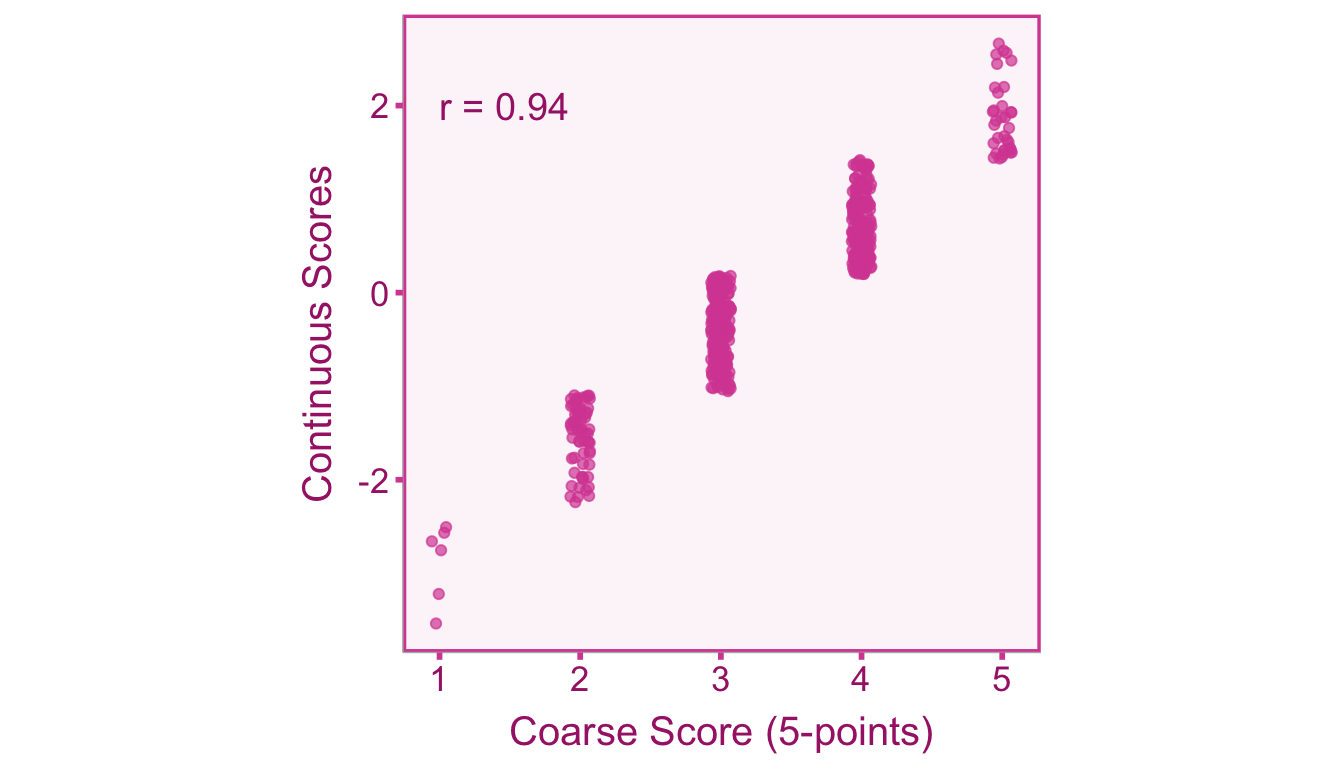
\includegraphics{chapters/07-scale-coarseness/07-scale-coarseness_files/figure-pdf/fig-coarse-self-1.pdf}

}

\caption{\label{fig-coarse-self}Scatterplot showing the correlation
between coarse scores (on a 5-point scale) and the underlying continuous
scores.}

\end{figure}%

\section{Correcting for Coarseness in
Correlations}\label{correcting-for-coarseness-in-correlations}

\subsection{Defining our Target
Quantity}\label{defining-our-target-quantity-2}

Our quantity of interest is the population correlation, \(\rho\),
between continuous independent variable, \(X\), and continuous dependent
variable, \(Y\). However, in a given study the measurement procedure may
produce coarse scores for \(X\) and \(Y\). We will denote coarse scores
with the subscript \(C\) We can model the relationship between the
observed sample correlation on coarse scores and the true population
correlation,

\[
r_{X_CY_C} = a\rho_{XY}+e.
\]

Where \(a\) is our artifact attenuation factor and \(e\) is our sampling
error term. We can obtain an unbiased estimate of the continuous
population correlation, \(\rho_{XY}\), by dividing the observed
correlation by an estimate of the attenuation factor,

\[
r_{XY} = \frac{r_{X_CY_C}}{\hat{a}}.
\]

\subsection{Artifact Correction for Coarseness}\label{sec-coarse-cor}

Correlating a coarse score with another variable will cause attenuation
of the correlation (MacCallum et al. 2002). Furthermore if we correlate
a coarse score with another coarse score than we will observe even more
attenuation (see Figure~\ref{fig-coarse-other}). There are two cases
that we can run into: 1) the univariate case where only one variable is
coarse and 2) the bivariate case where both variables are coarse.

\begin{figure}[H]

\centering{

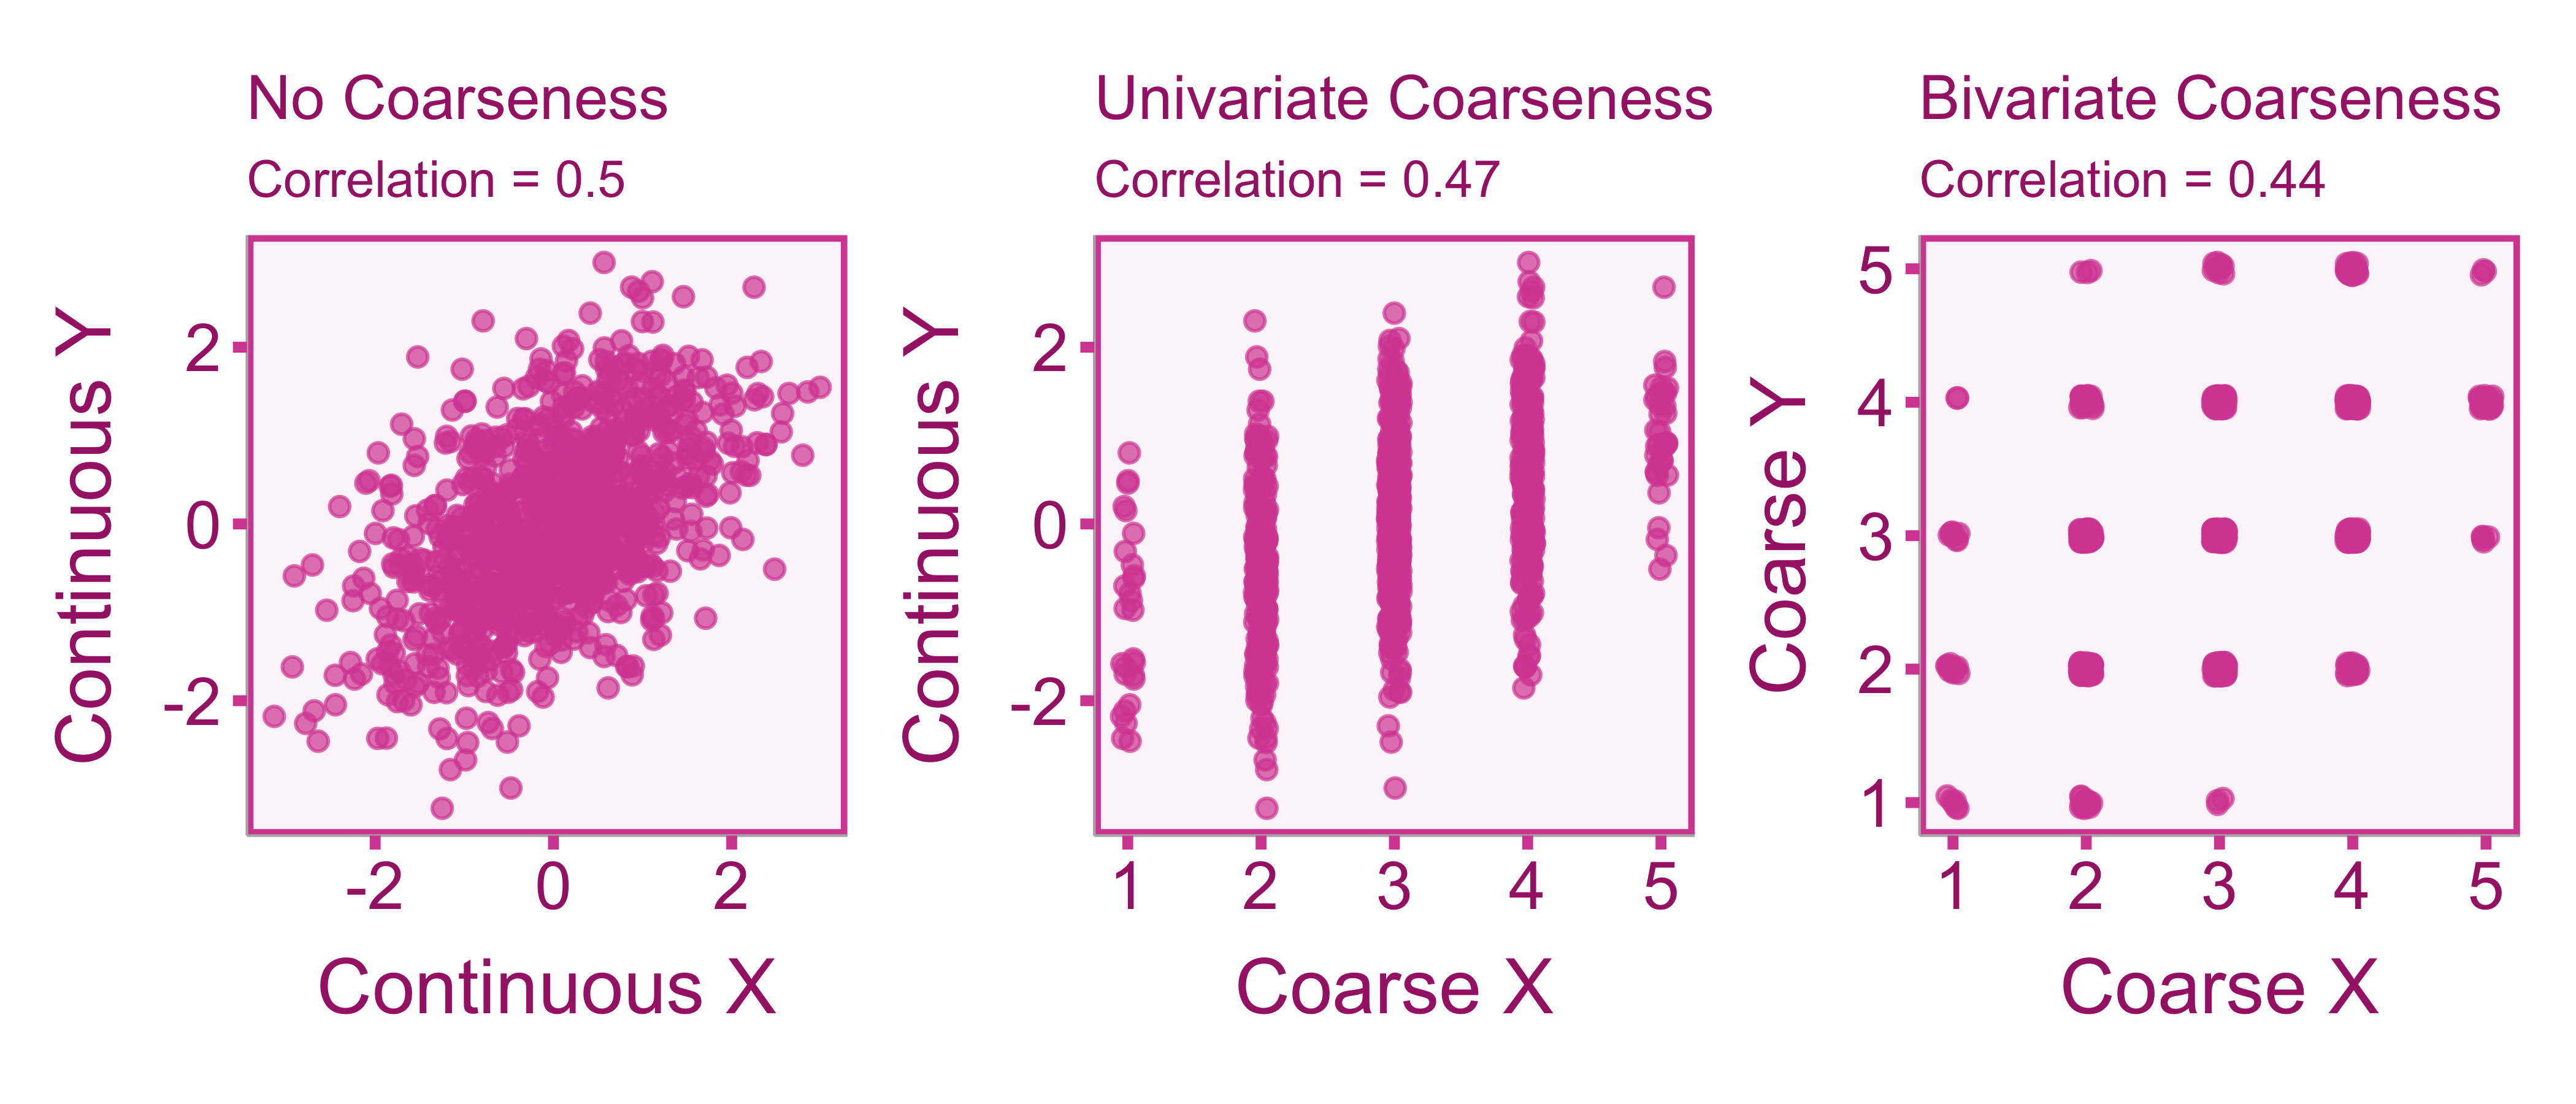
\includegraphics{chapters/07-scale-coarseness/07-scale-coarseness_files/figure-pdf/fig-coarse-other-1.pdf}

}

\caption{\label{fig-coarse-other}First plot (left to right) shows both
variables as continuous and normal. The second plot shows coarseness
(5-point scale) only on X, leaving Y continuous (\(r_{X_CY}=.47\)). Last
plot shows coarseness on both variables (\(r_{X_CY_C}=.47\)).}

\end{figure}%

To correct the correlation between coarse scores for \(X\) and \(Y\), we
need to know the correlation between coarse scores and their underlying
continuous scores (\(r_{XX_C}\) or \(r_{YY_C}\)). The calculation of the
correlation will require us two important assumptions:

\begin{enumerate}
\def\labelenumi{\arabic{enumi})}
\tightlist
\item
  The shape of the underlying distribution (i.e., normal or uniform).
\item
  The intervals between scale-points are equal.
\end{enumerate}

Based on these assumptions, Peters and Voorhis (1940) constructed a
table of correlations between coarse and continuous scores that is also
reported more recently by Aguinis, Pierce, and Culpepper (2009).
Table~\ref{tbl-coarse} is adapted from Peters and Voorhis (1940) and
displays the correlation values for uniform and normal distributions for
a given number of scale points. For the normal distribution correction,
its been shown that even in cases of extreme skew, these correction
factors perform well (Wylie 1976).

\begin{longtable}[]{@{}
  >{\centering\arraybackslash}p{(\columnwidth - 4\tabcolsep) * \real{0.2466}}
  >{\centering\arraybackslash}p{(\columnwidth - 4\tabcolsep) * \real{0.3699}}
  >{\centering\arraybackslash}p{(\columnwidth - 4\tabcolsep) * \real{0.3836}}@{}}
\caption{Correlations between continuous and coarse scores
(\(r_{XX_C}\)) from Peters and Voorhis
(1940)}\label{tbl-coarse}\tabularnewline
\toprule\noalign{}
\begin{minipage}[b]{\linewidth}\centering
Scale Points
\end{minipage} & \begin{minipage}[b]{\linewidth}\centering
Continuous-Coarse score Correlation (normal)
\end{minipage} & \begin{minipage}[b]{\linewidth}\centering
Continuous-Coarse score Correlation (uniform)
\end{minipage} \\
\midrule\noalign{}
\endfirsthead
\toprule\noalign{}
\begin{minipage}[b]{\linewidth}\centering
Scale Points
\end{minipage} & \begin{minipage}[b]{\linewidth}\centering
Continuous-Coarse score Correlation (normal)
\end{minipage} & \begin{minipage}[b]{\linewidth}\centering
Continuous-Coarse score Correlation (uniform)
\end{minipage} \\
\midrule\noalign{}
\endhead
\bottomrule\noalign{}
\endlastfoot
2 & .816 & .866 \\
3 & .859 & .943 \\
4 & .916 & .968 \\
5 & .943 & .980 \\
6 & .960 & .986 \\
7 & .970 & .990 \\
8 & .977 & .992 \\
9 & .982 & .994 \\
10 & .985 & .995 \\
11 & .988 & .996 \\
12 & .990 & .997 \\
13 & .991 & .997 \\
14 & .992 & .997 \\
15 & .994 & .998 \\
\end{longtable}

The correlations between coarse and continuous scores (\(r_{XX_C}\) and
\(r_{YY_C}\)) can be used to correct the correlation coefficient

\[
r_{XY} = \frac{r_{X_CY_C}}{r_{XX_C}r_{YY_C}}.
\]

Where \(r_{XX'}\) and \(r_{YY'}\) are the appropriate correction factors
from the table for \(x\) and \(y\). We must also adjust the sampling
variance as well,

\[
\sigma^2_{\varepsilon_c} = \frac{\sigma^2_{\varepsilon_o}}{a^2_x a^2_y}.
\]

\subsection{Correcting Correlations in
R}\label{correcting-correlations-in-r}

To correct scale coarseness in R, we can use the table in
Section~\ref{sec-coarse-cor}. Lets start by simulating a coarse data (5
scale-points for x and 7 scale-points for y) set of 500 individuals with
a true population correlation of \(\rho = .50\).

\begin{tcolorbox}[enhanced jigsaw, opacityback=0, coltitle=black, toprule=.15mm, colframe=quarto-callout-note-color-frame, bottomtitle=1mm, rightrule=.15mm, colbacktitle=quarto-callout-note-color!10!white, left=2mm, bottomrule=.15mm, breakable, title={Applied Example in R}, colback=white, opacitybacktitle=0.6, titlerule=0mm, arc=.35mm, leftrule=.75mm, toptitle=1mm]

Imagine that a researcher wants to relate depression and age. They
collect a sample of 1,000 people from the general population and
administer a very quick survey. Depression is measured based on a single
item from the patient health questionnaire (PHQ, Kroenke, Spitzer, and
Williams 2003) and age is measured in 5 age ranges:

\textbf{Over the last 2 weeks, how often have you been bothered by the
following problems?}

\textbf{What is your age?}

\begin{enumerate}
\def\labelenumi{\arabic{enumi}.}
\tightlist
\item
  Not at all
\item
  Several days
\item
  More than half the days
\item
  Nearly every day
\end{enumerate}

\begin{enumerate}
\def\labelenumi{\arabic{enumi}.}
\tightlist
\item
  1-20 years
\item
  21-40 years
\item
  41-60 years
\item
  61-80 years
\item
  81+ years
\end{enumerate}

Let's say we obtain a correlation of \(r_{X_C Y_C}=-.20\). Since the
correlation is computed on coarse scores, it is likely attenuated
relative to the correlation on each variables continuous underlying
scores. Therefore we can use the \texttt{correct\_r\_coarseness()}
function in the \texttt{psychmeta} package (Dahlke and Wiernik 2019) to
correct the correlation.

\begin{Shaded}
\begin{Highlighting}[]
\FunctionTok{library}\NormalTok{(psychmeta)}

\FunctionTok{correct\_r\_coarseness}\NormalTok{(}\AttributeTok{r =} \SpecialCharTok{{-}}\NormalTok{.}\DecValTok{20}\NormalTok{, }\CommentTok{\# observed correlation}
                     \AttributeTok{kx =} \DecValTok{5}\NormalTok{, }\CommentTok{\# 5 age range bins}
                     \AttributeTok{ky =} \DecValTok{4}\NormalTok{,  }\CommentTok{\# 4 PHQ item options}
                     \AttributeTok{n =} \DecValTok{1000}\NormalTok{, }\CommentTok{\# sample size}
                     \AttributeTok{dist\_x =} \StringTok{"unif"}\NormalTok{, }\CommentTok{\# assumed X distribution}
                     \AttributeTok{dist\_y =} \StringTok{"norm"}\NormalTok{) }\CommentTok{\# assumed Y distribution}
\end{Highlighting}
\end{Shaded}

\begin{verbatim}
  r_corrected var_e_corrected    n_adj
1  -0.2230339     0.001147251 788.0867
\end{verbatim}

We see a slight increase in the magnitude of the correlation with the
estimated correlation on continuous scores being \(r_{XY}=-.22\) and a
standard error of \(se(r_{XY})=\sqrt{.0011}=0.034\).

\end{tcolorbox}

\section{\texorpdfstring{Correcting for Coarseness in \emph{d}
values}{Correcting for Coarseness in d values}}\label{correcting-for-coarseness-in-d-values}

\subsection{Defining our Target
Quantity}\label{defining-our-target-quantity-3}

Our quantity of interest is the population standardized mean difference,
\(\delta_{gY}\), between groups \(A\) and \(B\) on continuous variable,
\(Y\). We can define the standardized mean difference on coarse scores
(\(d_{gY_C}\)) as,

\[
d_{gY_C} = a\delta_{gY}+\varepsilon.
\]

Where \(a\) is our coarseness biasing factor and \(\varepsilon\) is our
sampling error term. Ultimately, we can obtain an unbiased estimate of
the population standardized mean difference on continuous scores by
correcting the observed standardized mean difference as follows,

\[
d_{gY} = \frac{d_{gY_C}}{\hat{a}}.
\]

\subsection{Artifact Correction for
Coarseness}\label{artifact-correction-for-coarseness}

To correct a standardized mean difference for coarseness in dependent
variable, we can use the correlation between coarse scores and
continuous scores from Table~\ref{tbl-coarse},

\[
d_{gY} = \frac{d_{gY_C}}{r_{YY_C}}.
\]

Where \(r_{YY_C}\) is the appropriate correction factor from the table.
We must also adjust the standard error,

\[
se(d_{gY}) = \frac{se(d_{gY_C})}{r_{YY_C}}.
\]

\begin{tcolorbox}[enhanced jigsaw, opacityback=0, coltitle=black, toprule=.15mm, colframe=quarto-callout-note-color-frame, bottomtitle=1mm, rightrule=.15mm, colbacktitle=quarto-callout-note-color!10!white, left=2mm, bottomrule=.15mm, breakable, title={Applied Example in R}, colback=white, opacitybacktitle=0.6, titlerule=0mm, arc=.35mm, leftrule=.75mm, toptitle=1mm]

Let's say that a researcher wants to investigate gender differences in
depression. The researcher administers a survey to a sample of men and
women from the general population. Depression is measured based on a
single item from the patient health questionnaire (PHQ, Kroenke,
Spitzer, and Williams 2003):

\textbf{Over the last 2 weeks, how often have you been bothered by the
following problems?}

\begin{enumerate}
\def\labelenumi{\arabic{enumi}.}
\tightlist
\item
  Not at all
\item
  Several days
\item
  More than half the days
\item
  Nearly every day
\end{enumerate}

Let's say we obtain a standardized mean difference of \(d_{g Y_C}=.25\),
slightly favoring women. Since there is currently no
\texttt{correct\_d\_coarseness()} function in \texttt{psychmeta}, we can
simply correct the correlation with base R. again however we will need t
in the \texttt{psychmeta} package (Dahlke and Wiernik 2019) to correct
the correlation.

\begin{Shaded}
\begin{Highlighting}[]
\FunctionTok{library}\NormalTok{(psychmeta)}

\NormalTok{dgYc }\OtherTok{\textless{}{-}}\NormalTok{ .}\DecValTok{25} \CommentTok{\# standardized mean difference on coarse scores}
\NormalTok{se.dgYc }\OtherTok{\textless{}{-}}\NormalTok{ .}\DecValTok{10} \CommentTok{\# standardized mean difference on coarse scores}
\NormalTok{rYYc }\OtherTok{\textless{}{-}}\NormalTok{ .}\DecValTok{916}

\NormalTok{dgY }\OtherTok{\textless{}{-}}\NormalTok{ dgYc }\SpecialCharTok{/}\NormalTok{ rYYc }\CommentTok{\# correct d}
\NormalTok{se.dgY }\OtherTok{\textless{}{-}}\NormalTok{ se.dgYc }\SpecialCharTok{/}\NormalTok{ rYYc }\CommentTok{\# correct se}

\CommentTok{\# print results}
\FunctionTok{cbind}\NormalTok{(dgY, se.dgY)}
\end{Highlighting}
\end{Shaded}

\begin{verbatim}
           dgY    se.dgY
[1,] 0.2729258 0.1091703
\end{verbatim}

We see a slight increase in the magnitude of the correlation with the
estimated correlation on continuous scores being \(d_{gY}=.27\) and a
standard error of \(se(d_{gY})=.109\).

\end{tcolorbox}

\bookmarksetup{startatroot}

\chapter{Introduction to Selection
Effects}\label{introduction-to-selection-effects}

\bookmarksetup{startatroot}

\chapter{Direct Selection}\label{sec-direct_range_restriction}

\section{Introduction}\label{introduction-6}

Direct selection occurs when subjects are explicitly selected based on
some eligibility criterion on the variables of interest (rather than a
third variable). Range restriction is a form of selection bias that
describes a situation where there is less variation in our sample then
there is in the population. Whereas range enhancement indicates that
there is \emph{more} variation in a sample then there is in the
population. Direct range restriction/enhancement biases the variances
and effect size estimates.

\section{An Example of Direct Range
Restriction}\label{an-example-of-direct-range-restriction}

Imagine a tech company that wants to assess the correlation between
years of experience and programming proficiency for their software
engineers. They have two primary divisions: Division A and Division B.
Division A primarily hires entry-level software engineers, with less
than 3 years of experience. Division B, on the other hand, hires
experienced software engineers with more than 3 years of experience. The
company decides to conduct a study to assess the correlation between
years of experience and programming proficiency. However, they only
collect data from Division A due to logistical reasons, assuming that
the relationship found there would be represent the entire company. In
this scenario, direct range restriction occurs because the sample used
for the study (Division A) represents a narrow range of years of
experience (0-3 years) compared to the broader range present in the
entire company (0+ years). Consequently, the standard deviation will be
smaller in the sample then it would if we had sampled from the entire
company. As we will see in later sections of this chapter, the observed
correlation between years of experience and programming proficiency
would be attenuated, underestimating the true correlation.

\section{A Direct Selection Function}\label{a-direct-selection-function}

A selection function described here is a type of indicator function that
represents the mechanism of which observations are selected into a given
sample. In the case of \emph{direct} selection, the selection will be a
function of the of the variable of interest, \(X\). We will denote a
selection function as \(\mathcal{S}(X)\). The output of the selection
function will be a binary: either the individual is selected
\(\mathcal{S}(X)=1\) or rejected \(\mathcal{S}(X)=0\) (see
Figure~\ref{fig-direct-select-diag}).

\begin{figure}[H]

\centering{

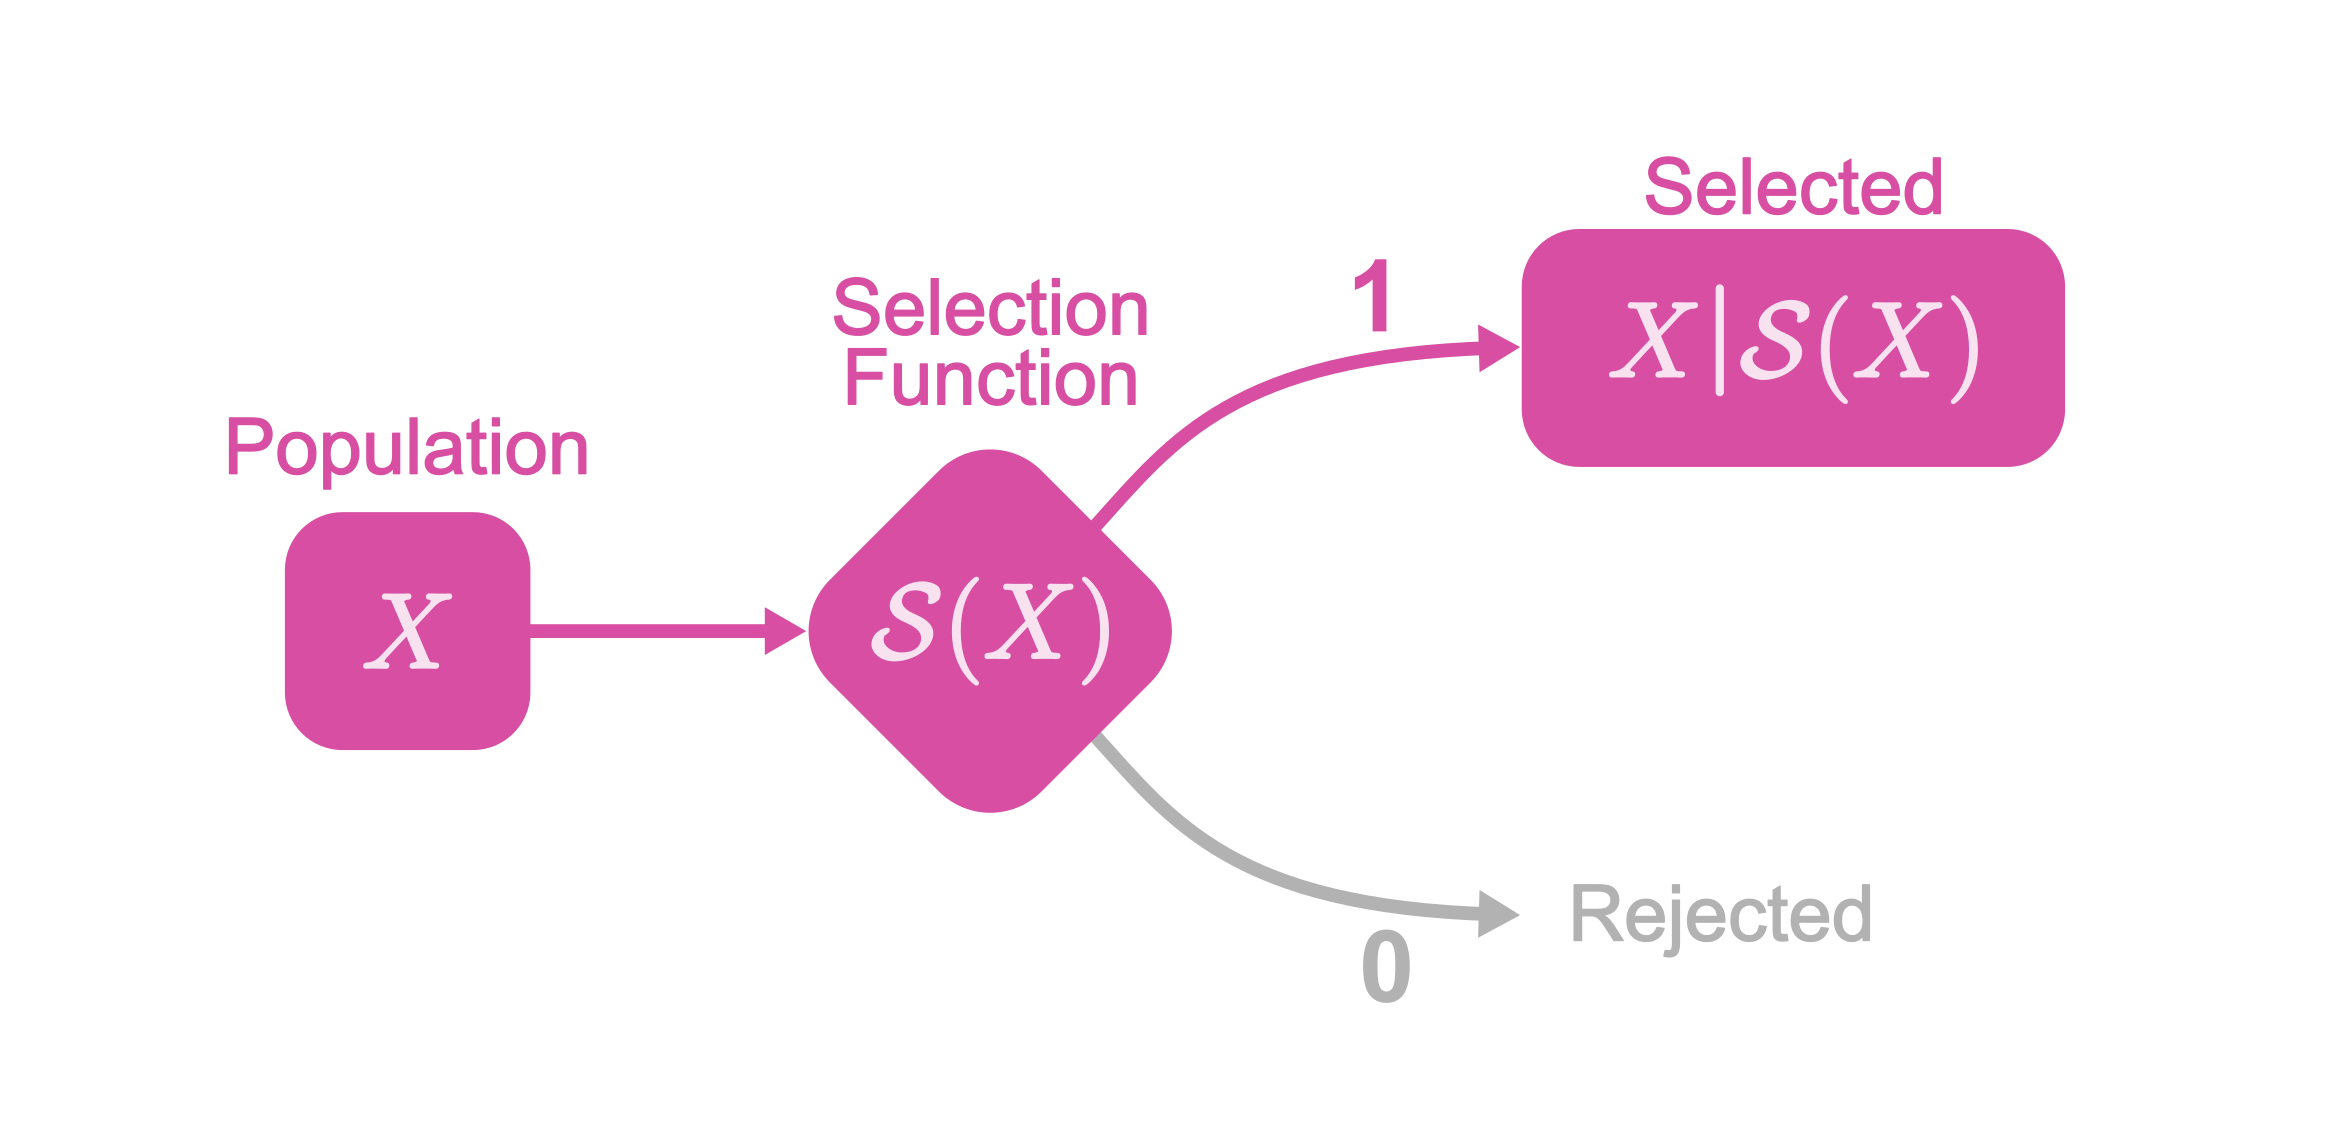
\includegraphics{chapters/09-direct-selection/figure/direct_select_diagram.png}

}

\caption{\label{fig-direct-select-diag}Diagram illustrating the direct
selection function. The variable, \(X\), in the population is selected
based on a function of itself. Therefore the variable under selection is
conditional on the selection procedure \(X|\mathcal{S}(X)\).}

\end{figure}%

The functional form of the selection function is going to be described
by some inequality of \(X\). The inequality will be dependent on the
research context (e.g., the sampling procedure).

\begin{tcolorbox}[enhanced jigsaw, opacityback=0, coltitle=black, toprule=.15mm, colframe=quarto-callout-tip-color-frame, bottomtitle=1mm, rightrule=.15mm, colbacktitle=quarto-callout-tip-color!10!white, left=2mm, bottomrule=.15mm, breakable, title={A Simple Example}, colback=white, opacitybacktitle=0.6, titlerule=0mm, arc=.35mm, leftrule=.75mm, toptitle=1mm]

Let's define the selection function as

\[\mathcal{S}(X) = \begin{cases}1 & \text{if }X>3 \text{ and } X<8 \\ 0 & \text{if }X\leq3 \text{ and } X\geq8  \end{cases}\]
then let's say \(X\) contains the following observations, \[
X = [1,2,3,4,5,6,7,8,9,10]
\]

the selection function would then return,

\[
\mathcal{S}(X) =  [0,0,0,1,1,1,1,0,0,0]
\] therefore \(X\) given selection on \(X\) would be,

\[
X|\mathcal{S}(X) =  [4,5,6,7]
\]

\end{tcolorbox}

Direct selection on \(X\) will have a fairly straight forward effect on
the distribution of \(X\). The probability density function of \(X\)
(\(f(X)\)) under direct selection can be formally defined as,

\[
f\left(X|\mathcal{S}(X)\right) = f(X) \mathcal{S}(X)
\]

We can visualize the distribution under direct selection in
Figure~\ref{fig-pdf}. Note that this is a simple case where selection is
done on a single variable (i.e., univariate direct selection). In
practice, selection is often a function of multiple variables. For
instance, bivariate direct selection occurs when the selection is a
function of both variables of interest, \(\mathcal{S}(X,Y)\).

\begin{figure}[H]

\centering{

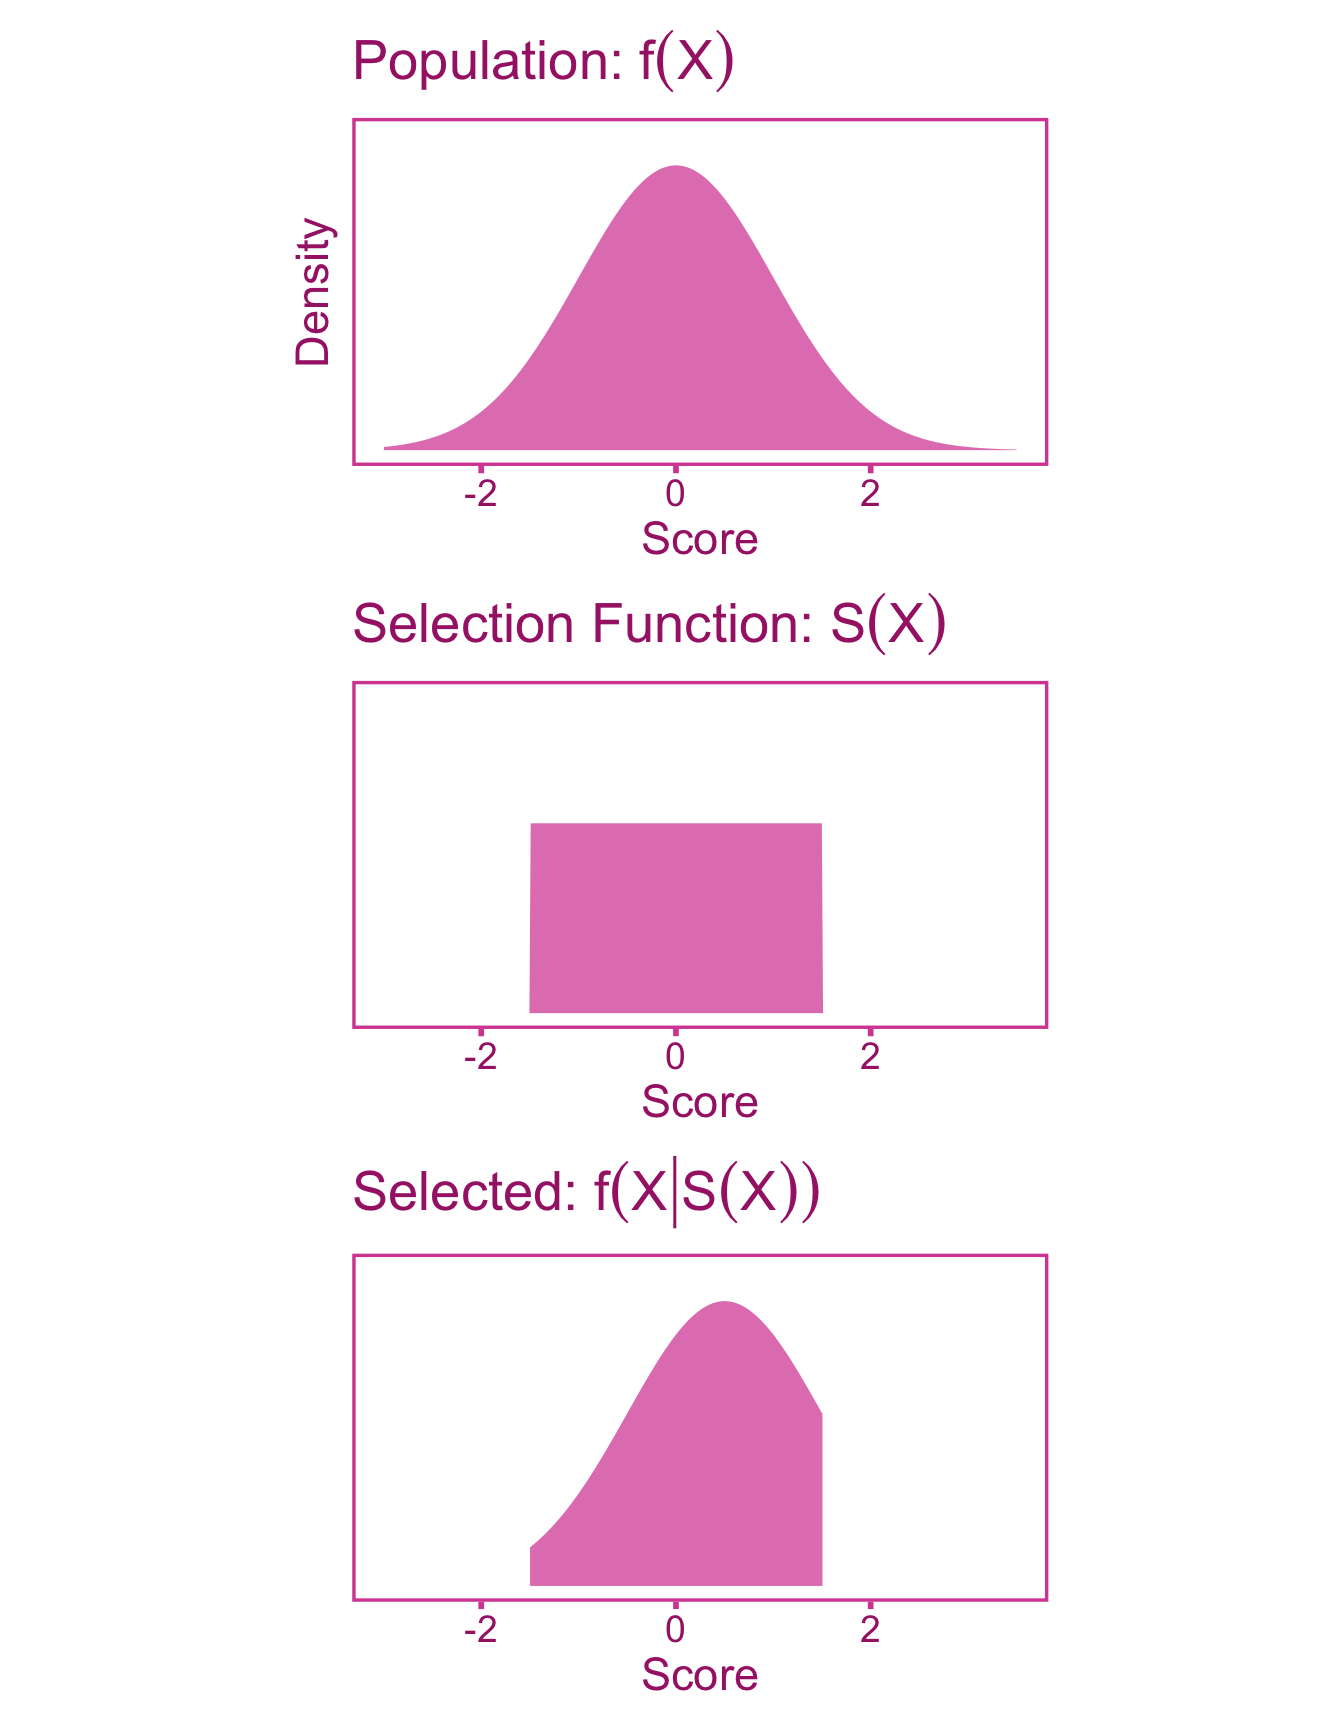
\includegraphics{chapters/09-direct-selection/09-direct-selection_files/figure-pdf/fig-pdf-1.pdf}

}

\caption{\label{fig-pdf}Visualizing direct selection with an example
probability density and selection function. Top panel shows a normally
distribution of \(X\) within the population. The middle panel shows the
selection function. The selection function is based on the inequality,
\(-1.0<X<1.5\). The bottom panel shows the distribution of \(X\) after
selecting on \(X\) (i.e., \(X|\mathcal{S}(X)\)).}

\end{figure}%

\section{\texorpdfstring{Quantifying Direct Selection-Induced
Restriction/Enhancement with the
\emph{u}-ratio}{Quantifying Direct Selection-Induced Restriction/Enhancement with the u-ratio}}\label{quantifying-direct-selection-induced-restrictionenhancement-with-the-u-ratio}

The distribution of scores in the population of individuals will exhibit
a greater (or lesser) degree of variability compared to the population
that meets the selection criterion. Therefore the standard deviation of
scores in the target population (\(\sigma_{X}\)) will differ from that
of the population under direct selection on \(X\)
(\(\sigma_{X|\mathcal{S}(X)}\)). To index the difference between the two
standard deviations, we can calculate the \(u\)-ratio Wiernik and Dahlke
(2020). The \(u\)-ratio is defined as the ratio between the standard
deviations of the population (\(\sigma_{X|\mathcal{S}(X)}\)) under
selection and the target population (\(\sigma_{X}\)) such that,

\[
\upsilon_X = \frac{\sigma_{X|\mathcal{S}(X)}}{\sigma_{X}}
\] Where \(\upsilon_{X}\) denotes the population \(u\)-ratio. The
\(u\)-ratio in cases of range restriction will exist in the interval
(0--1). Conversely, when the \(u\)-ratio is greater than 1 it is
indicative of range enhancement. For a sample, the \(u\)-ratio is
calculated from sample standard deviations,

\[
u_X = \frac{S_{X|\mathcal{S}(X)}}{S_X}
\]

Where \(u_{X}\) denotes the sample \(u\)-ratio. The target population
standard deviation is often quite difficult to estimate since generally
we do not have access to an estimate of the population of interest.
However, the unrestricted standard deviation can be estimated from some
reference or norm study that is representative of the population of
interest. This often comes in the form of standardization samples or
norm samples (obtained from test manuals) if the population of interest
is the general population. For example, the distribution full-scale IQ
scores derived from the Wechsler Adult Intelligence Test has a standard
deviation of 15 in the US population (Wechsler 2008). We can use this
estimate as the standard deviation for the target population. Lets say
we select a sample from members of Mensa, a high IQ society, where
members are specifically selected on the basis high IQ scores. If the
standard deviation of Mensa members is 5, then the \(u\)-ratio would be,

\[
u_x = \frac{S_{X|\mathcal{S}(X)}}{S_X} = \frac{5}{15}= .33\, .
\]

If an estimate of the population standard deviation is not readily
available, then a reliability coefficient from the reference sample and
the sample under selection can be used to estimate the \(u\)-ratio,

\[
u_X = \sqrt{\frac{1-r_{XX'}}{1-r_{XX'|\mathcal{S}(X)}}}.
\]

Where \(r_{XX'|\mathcal{S}(X)}\) and \(r_{XX'}\) are the reliability
estimates within the selected and reference sample respectively.

\section{Correcting Correlations for Direct Range
Restriction}\label{correcting-correlations-for-direct-range-restriction}

\subsection{Defining our Target
Quantity}\label{defining-our-target-quantity-4}

We want to estimate the correlation in the target population between
true scores of the independent (\(T\)) and dependent variable (\(U\)).
Within a study that suffers from direct selection and measurement error,
the observed score correlation will be biased relative to our target
true score population correlation, \(\rho_{TU}\). We can model observed
score correlations under univariate direct selection as,

\[
r_{XY|\mathcal{S}(X)} = a \rho_{TU} + e
\]

or under bivariate direct selection,

\[
r_{XY|\mathcal{S}(X,Y)} = a \rho_{TU} + e.
\]

Where \(a\) is the artifact attenuation/inflation factor and \(e\) is
the sampling error term. In either case, an unbiased estimate of the
total population true score correlation can be estimated by dividing by
an estimate of \(a\),

\[
r_{XY|\mathcal{S}(X)} = a \rho_{TU} + e
\]

or

\[
r_{XY|\mathcal{S}(X,Y)} = a \rho_{TU} + e.
\]

\subsection{Artifact Correction for Correlations}\label{sec-corr-DDR}

\subsubsection*{The Univariate Case}\label{the-univariate-case-1}
\addcontentsline{toc}{subsubsection}{The Univariate Case}

Range restriction (or enhancement) in either the independent or
dependent variable will induce bias into the correlation coefficient.
Let us consider a case where a study directly selects on \(X\) and not
\(Y\). It is important to note, that if there is direct selection one of
the two variables, then there will be indirect selection in the other
variable too if the two are correlated. This would suggest that if
\(u_X\neq 1\) and \(\rho_{XY}\neq 0\) then \(u_Y\neq 1\). Lets visualize
the correlation between independent (\(X\)) and dependent (\(Y\))
variables under univariate direct range restriction (see
Figure~\ref{fig-uvdrr}) by only selecting individuals above some cut off
such that,

\[
\mathcal{S}(X) = \begin{cases}1 & \text{if }X\geq-.50\\ 0 & \text{if }X<-.50  \end{cases}
\]

The scores of individuals that have been selected will show less
variance than the population pool. Specifically, the scenario below
shows a \(u\)-ratio of \(u_X=0.69\) in the independent variable. We see
in Figure~\ref{fig-uvdrr} that the correlation in the restricted scores
(\(r_{XY|\mathcal{S}(X)}\)) are attenuated relative to the unrestricted
correlation (\(r_{XY}\), indicative of \(a<1\)).

\begin{figure}[H]

\centering{

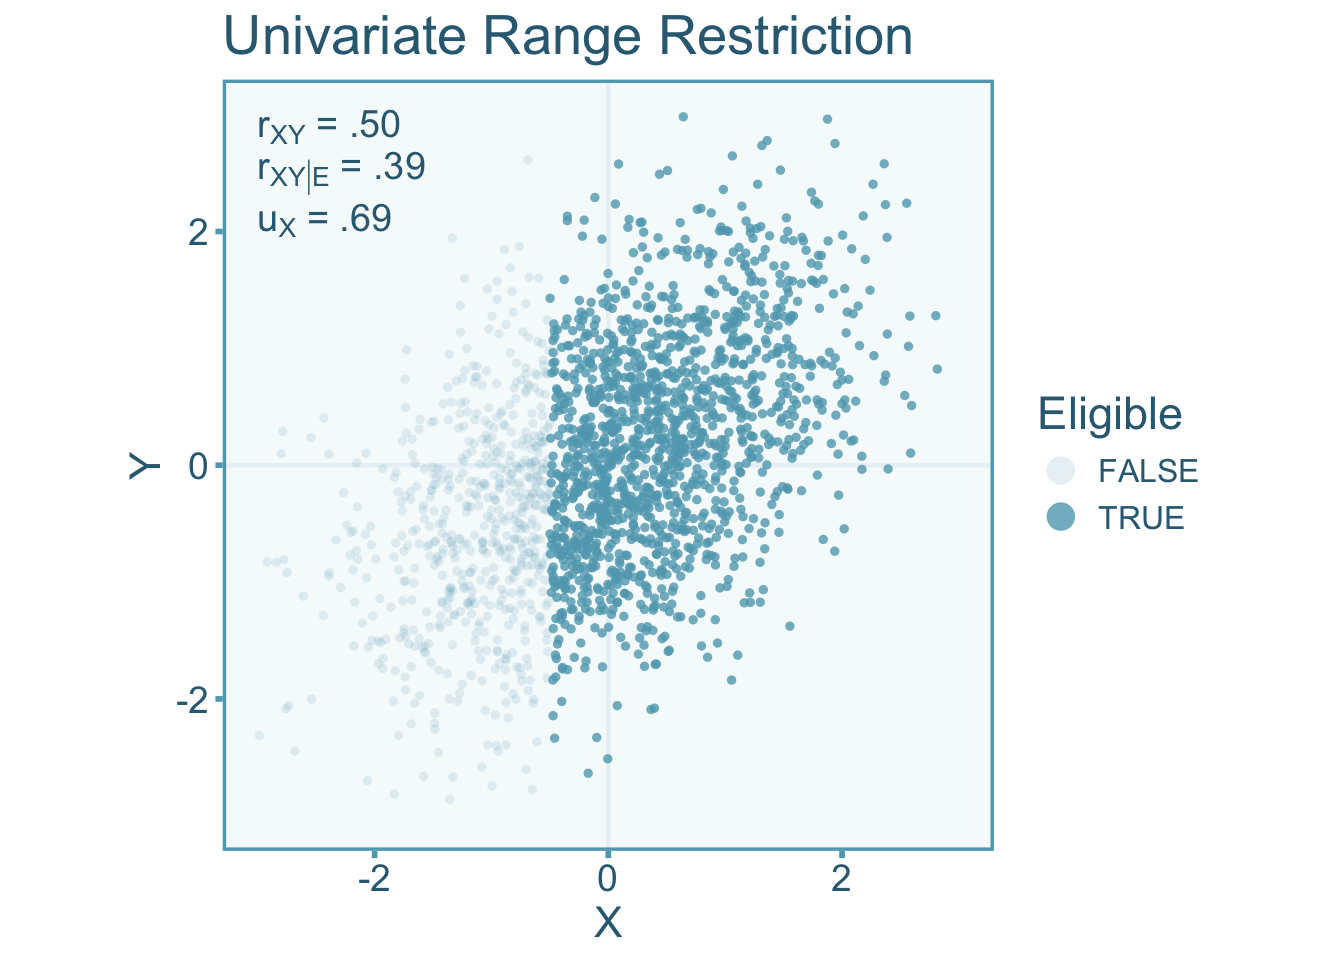
\includegraphics{chapters/09-direct-selection/09-direct-selection_files/figure-pdf/fig-uvdrr-1.pdf}

}

\caption{\label{fig-uvdrr}Scatterplot showing a correlation between
\(X\) and \(Y\) under univariate direct range restriction. Dark blue
dots indicate the selected sample and the transparent dots indicate the
rejected sample.}

\end{figure}%

We can also visualize what happens to the correlation when the range is
enhanced. Enhancement can be accomplished by selecting individuals at
the ends of the distribution (Taylor and Griess 1976). Therefore we can
define the selection function for Figure~\ref{fig-uvdre} as,

\[
\mathcal{S}(X) = \begin{cases}1 & \text{if }X\leq-.50 \text{ or } X\geq.50\\0 & \text{if }X>-.50 \text{ or } X<.50\end{cases}
\]

In the visualization below, we see an opposite effect on the
correlation, that is, an inflation of the unrestricted correlation
rather than an attenuation (indicating \(a>1\)) like we see under range
restriction. The scenario below has a \(u\)-ratio \(u_X=1.26\) in the
independent variable.

\begin{figure}[H]

\centering{

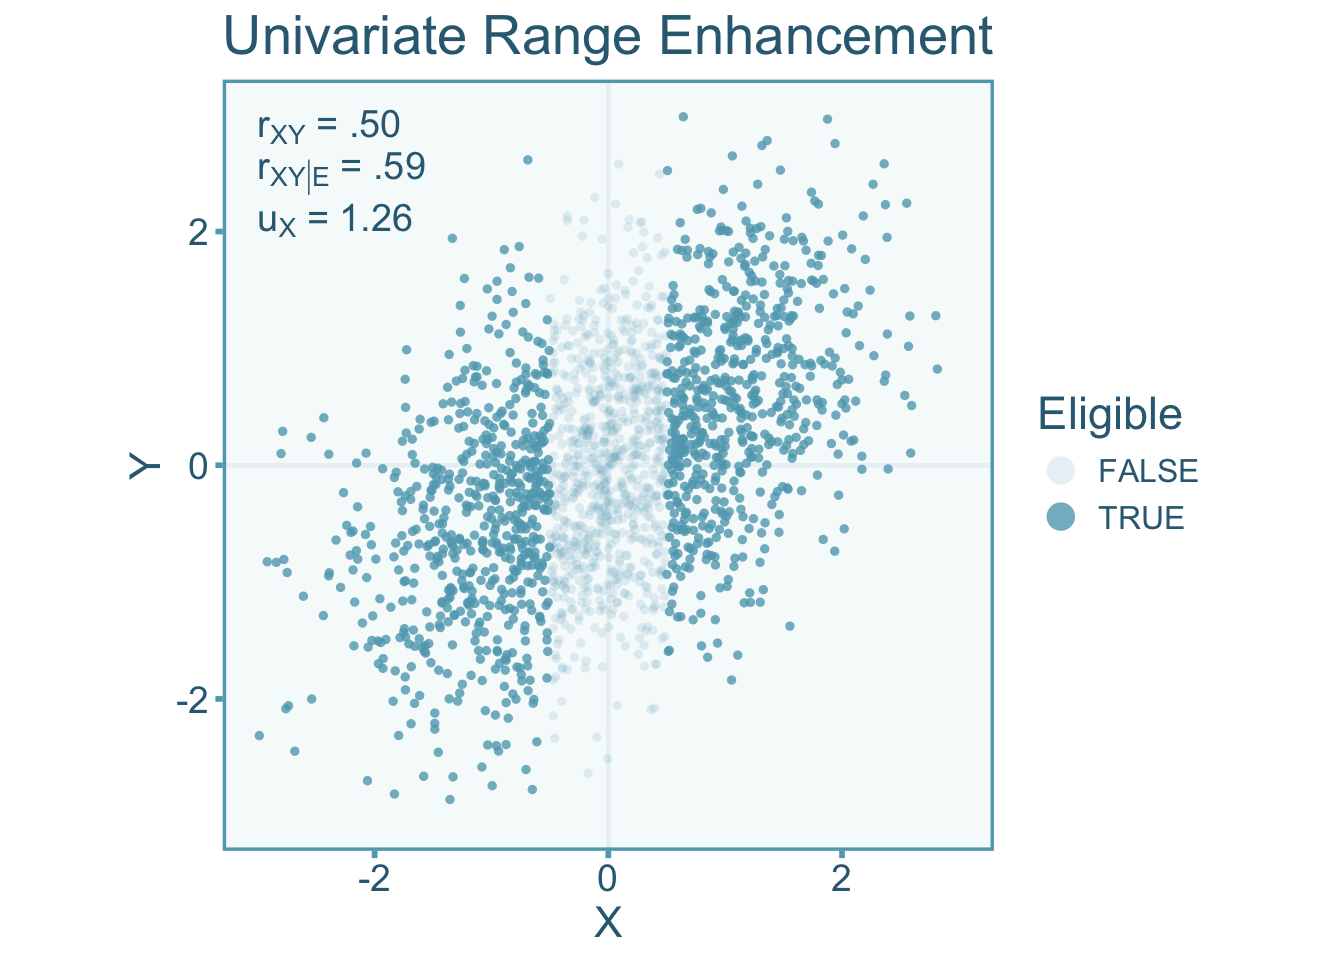
\includegraphics{chapters/09-direct-selection/09-direct-selection_files/figure-pdf/fig-uvdre-1.pdf}

}

\caption{\label{fig-uvdre}Scatterplot showing a correlation between
\(X\) and \(Y\) under univariate direct range enhancement. Dark blue
dots indicate the selected sample and the transparent dots indicate the
rejected sample.}

\end{figure}%

It starts to become apparent that if \(u_X>1\) (i.e.,
\(S_X>S_{X|\mathcal{S}(X)}\)) the observed correlation is inflated and
when \(u_X<1\) it becomes attenuated (Sackett and Yang 2000).

The attenuation/inflation of the correlation is dependent on the
magnitude of the correlation, this is due to the fact that selection
occurs on \(X\) \emph{and} \(X\) is correlated with \(Y\), there will
also be indirect range restriction in \(Y\). Therefore unlike other
artifacts that have been discussed so far, range restriction/enhancement
depends not only on the artifact value (i.e., the \(u\)-ratio), but also
on the restricted correlation (J. E. Hunter, Schmidt, and Le 2006). The
attenuation/inflation factor can be estimated as (adapted from equation
4, J. E. Hunter, Schmidt, and Le 2006),

\[
\hat{a} = u_X \sqrt{1+r_{XY|\mathcal{S}(X)}^2\left(\frac{1}{u_X}-1\right)}
\]

A bias correction formula for univariate direct selection was first
developed by Pearson (1903) and also provided more recently by J. E.
Hunter, Schmidt, and Le (2006) and Wiernik and Dahlke (2020). To correct
for the systematic bias in correlations, we can divide the correlation
under selection by the attenuation factor,

\begin{equation}\phantomsection\label{eq-univariate}{
r_{XY} = \frac{r_{XY|\mathcal{S}(X)}}{\hat{a}} = \frac{r_{XY|\mathcal{S}(X)}}{u_X\sqrt{1+r_{XY|\mathcal{S}(X)}^2\left(\frac{1}{u^2_X}-1\right)}}.
}\end{equation}

Where the standard error of the corrected correlation is,

\begin{equation}\phantomsection\label{eq-univariate-se}{
se(r_{XY}) = \frac{se\left(r_{XY|\mathcal{S}(X)}\right)}{\hat{a}}.
}\end{equation}

If we want to also correct for measurement error in both samples, then
we can also incorporate the reliability into these equations. Note that
the following equations will incorporate the reliability within the
selected sample (\(r_{XX'|\mathcal{S}(X)}\)) rather than the reference
sample (\(r_{XX'}\)). If the reliability coefficient comes from the
reference sample, then we can estimate the selected (restricted or
enhanced) sample reliability with the corresponding \(u\)-ratio,

\begin{equation}\phantomsection\label{eq-samp-reliability}{
r_{XX'|\mathcal{S}(X)} = 1-\frac{1-r_{XX'}}{u^2_X}.
}\end{equation}

Then we can use the reliability and \(u\)-ratios simultaneously to
calculate a new attenuation/inflation factor that accounts for both bias
in measurement error and direct selection,

\[
\hat{a} = u_X\sqrt{1-u_X^2(1-r_{XX'|\mathcal{S}(X)})}\sqrt{r_{YY'|\mathcal{S}(X)}+r_{XY|\mathcal{S}(X)}^2\left(\frac{1}{u^2_X}-1\right)}.
\]

In the following equation to obtain an unbiased estimate of the true
score unrestricted population correlation (adapted from table 3, Wiernik
and Dahlke 2020),

\[
\small{r_{TU}=\frac{r_{XY|\mathcal{S}(X)}}{\hat{a}} =\frac{r_{XY|\mathcal{S}(X)}}{u_X\sqrt{1-u_X^2(1-r_{XX'|\mathcal{S}(X)})}\sqrt{r_{YY'|\mathcal{S}(X)}+r_{XY|\mathcal{S}(X)}^2\left(\frac{1}{u^2_X}-1\right)}}}
\]

Where the standard error can be corrected similarly,

\[
se(r_{TU}) = \frac{se(r_{XY|\mathcal{S}(X)})}{\hat{a}}
\]

There are three important things to note about the equations in this
section: 1) these corrections assume linearity and homoskedasticity in
the target population population, 2) all these corrections show
selection on the independent variable, \(X\), however it does not matter
whether univariate selection is on \(X\) or \(Y\), the corrections can
be applied in the same fashion (just remember to flip \(X\) and \(Y\)
and vice versa in the equations), 3) The corrections assume that any
range restriction/enhancement observed in the non-selection variable (in
our example this would be \(Y\)) is mediated by the range
restriction/enhancement in the variable under selection (i.e., \(X\)).

\begin{tcolorbox}[enhanced jigsaw, opacityback=0, coltitle=black, toprule=.15mm, colframe=quarto-callout-note-color-frame, bottomtitle=1mm, rightrule=.15mm, colbacktitle=quarto-callout-note-color!10!white, left=2mm, bottomrule=.15mm, breakable, title={Applied Example in R}, colback=white, opacitybacktitle=0.6, titlerule=0mm, arc=.35mm, leftrule=.75mm, toptitle=1mm]

To continue with our example of Mensa members (a high IQ society), let's
say a researcher wants to know the correlation between IQ and test
anxiety. The researcher conduct's a study on a sample of 100 Mensa
members and finds a sample mean IQ of \(135\) and a standard deviation
of \(S_{X|\mathcal{S}(X)}=5\). Since the mean IQ in the general
population is 15, the \(u\)-ratio is computed as \(u_X=.333\). The
researcher then finds a correlation of \(r_{XY|\mathcal{S}(X)}=-.15\)
between IQ test scores and test anxiety. The reliability of the IQ test
and the anxiety measure is \(r_{XX'|\mathcal{S}(X)}=.85\) and
\(r_{YY'|\mathcal{S}(X)}=.80\), respectively.

In R, we can correct the correlation by using the \texttt{correct\_r}
function in the \texttt{psychmeta} package (Dahlke and Wiernik 2019).
The \texttt{correction\ =\ \textquotesingle{}uvdrr\_x\textquotesingle{}}

\begin{Shaded}
\begin{Highlighting}[]
\FunctionTok{library}\NormalTok{(psychmeta)}

\FunctionTok{correct\_r}\NormalTok{(}\AttributeTok{correction =} \StringTok{\textquotesingle{}uvdrr\_x\textquotesingle{}}\NormalTok{,}
          \AttributeTok{rxyi =} \SpecialCharTok{{-}}\NormalTok{.}\DecValTok{15}\NormalTok{,  }\CommentTok{\# restricted correlation}
          \AttributeTok{ux =}\NormalTok{ .}\DecValTok{333}\NormalTok{,   }\CommentTok{\# u ratio of IQ scores}
          \AttributeTok{rxx =}\NormalTok{ .}\DecValTok{85}\NormalTok{,   }\CommentTok{\# reliability of IQ scores}
          \AttributeTok{ryy =}\NormalTok{ .}\DecValTok{80}\NormalTok{,   }\CommentTok{\# reliability of test anxiety measure}
          \AttributeTok{n =} \DecValTok{100}\NormalTok{)    }\CommentTok{\# sample size}
\end{Highlighting}
\end{Shaded}

\begin{verbatim}
Correlations Corrected for Measurement Error and Univariate Direct Range Restriction:
---------------------------------------------------------------------------------------
   value CI_LL_95 CI_UL_95   n n_effective
1 -0.459    -0.78     0.16 100        10.6
\end{verbatim}

The true score correlation in the target population is estimated to be
\(r_{TU} = .46\, [-.16,\, .78]\).

\end{tcolorbox}

\subsubsection*{The Bivariate Case}\label{the-bivariate-case-1}
\addcontentsline{toc}{subsubsection}{The Bivariate Case}

Bivariate direct range restriction/enhancement occurs when selection
occurs on both variables of interest, therefore the selection function
will be a function of \(X\) \emph{and} \(Y\). Let's visualize the
correlation between independent (\(X\)) and dependent (\(Y\)) variables
under bivariate range restriction by only selecting individuals above
some cut off point for both \(X\) and \(Y\) (see
Figure~\ref{fig-bvdrr}). For this example the selection function is

\[
\mathcal{S}(X,Y) = \begin{cases}1 & \text{if } X\geq -.5 \text{ and }Y\geq-.5\\ 0 & \text{if }X<-.5  \text{ and }Y<-.5 \end{cases}
\]

The scores of individuals that have been selected will show less
variance than the entire pool of individuals. Specifically, the scenario
below shows a \(u\)-ratio of about 0.70 in the independent variable and
dependent variables. We see in the figure that the correlation in the
restricted sample (\(r_{XY|\mathcal{S}(X,Y)}\)) is attenuated relative
to the unrestricted correlation (\(r_{XY}\)).

\begin{figure}[H]

\centering{

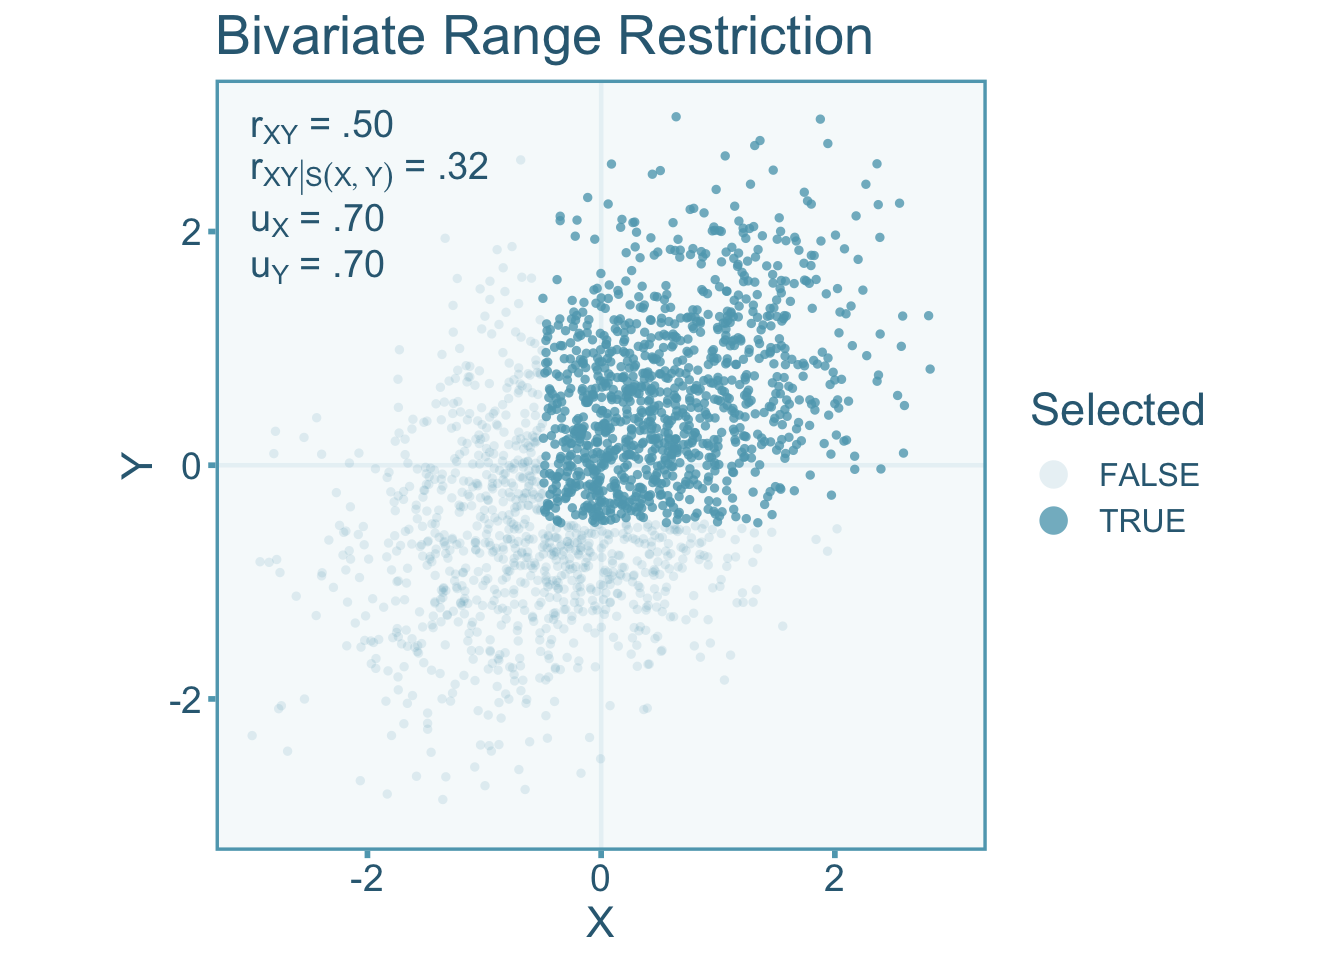
\includegraphics{chapters/09-direct-selection/09-direct-selection_files/figure-pdf/fig-bvdrr-1.pdf}

}

\caption{\label{fig-bvdrr}Scatterplot showing a correlation between
\(X\) and \(Y\) under bivariate direct range restriction. Dark blue dots
indicate the selected sample and the transparent dots indicate the
rejected sample.}

\end{figure}%

Likewise let's visualize what happens to the correlation when the range
is enhanced. Enhancement in both variables can be accomplished by
selecting individuals at the ends of the distribution of \(X\) and
\(Y\). Therefore we can define the selection function as,

\[
\small{\mathcal{S}(X,Y) = \begin{cases}1 & \text{if } (X\leq -.5 \text{ or } X\geq .5) \text{ and } (Y\leq -.5 \text{ or } Y\geq .5) \\ 0 & \text{if }(X>-.5 \text{ or }X<.5)  \text{ and }(Y>-.5 \text{ or }Y<.5) \end{cases}}
\]

Note that this type of selection would be exceedingly rare to see in
practice. In Figure~\ref{fig-bvdre}, we see inflation of the enhanced
correlation relative to the target correlation. The scenario below has a
\(u\)-ratio of about 1.32 in both the independent variable and dependent
variable.

\begin{figure}[H]

\centering{

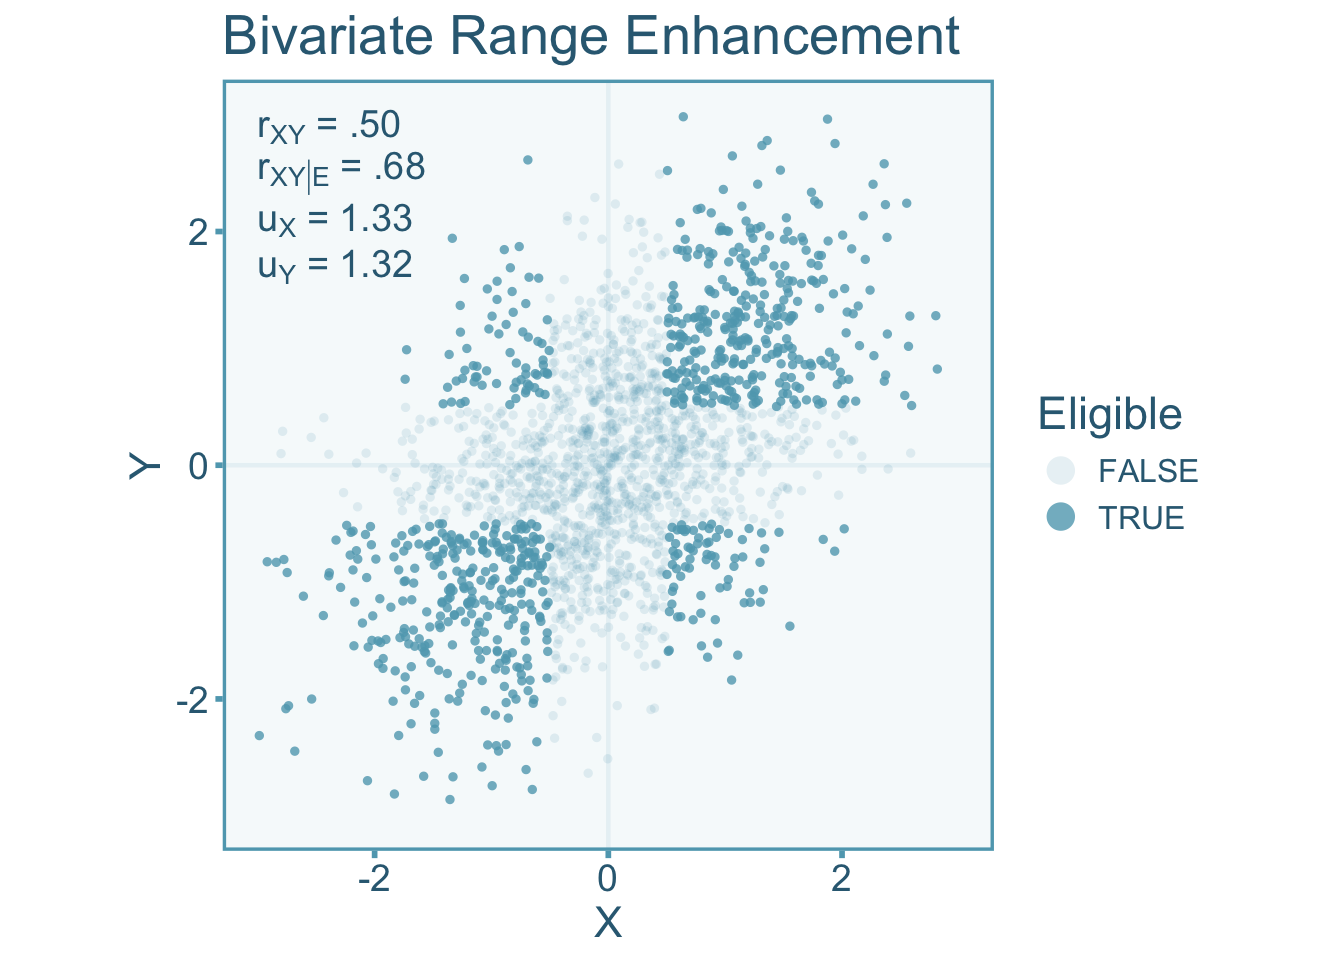
\includegraphics{chapters/09-direct-selection/09-direct-selection_files/figure-pdf/fig-bvdre-1.pdf}

}

\caption{\label{fig-bvdre}Scatterplot showing a correlation between
\(X\) and \(Y\) under bivariate direct range enhancement. Dark blue dots
indicate the selected sample and the transparent dots indicate the
rejected sample.}

\end{figure}%

A bias correction formula for bivariate range restriction is much more
complicated than the univariate formulation. To break down the
correction formula into simpler parts, let us first define a factor we
will denote with the Greek letter \(\psi\),

\begin{equation}\phantomsection\label{eq-biv-1}{
\psi = \frac{u_X u_Y\left(r_{XY|\mathcal{S}(X,Y)}^2-1\right)}{2r_{XY|\mathcal{S}(X,Y)}}
}\end{equation}

This factor contains all the parameters needed to correct the
correlation coefficient under direct selection. An unbiased estimate of
the target population correlation can obtained by the following
correction formula (adapted from table 3 Wiernik and Dahlke 2020),

\begin{equation}\phantomsection\label{eq-biv-2}{
r_{XY} = \psi + \text{sign}\left[r_{XY|\mathcal{S}(X,Y)}\right]\sqrt{\psi^2+1}
}\end{equation}

Where the standard error can be computed from calculating the artifact
factor (\(a\)) from the corrected and restricted/enhanced correlation,

\begin{equation}\phantomsection\label{eq-biv-se}{
se(r_{XY}) = \frac{se\left(r_{XY|\mathcal{S}(X,Y)}\right)}{\hat{a}}= \frac{se\left(r_{XY|\mathcal{S}(X,Y)}\right)}{\left[\frac{r_{XY|\mathcal{S}(X,Y)}}{r_{XY}}\right]}.
}\end{equation}

Now we can also incorporate measurement error into the correction
formula. Note that the following equations will incorporate the
reliability within the selected sample (\(r_{XX'|\mathcal{S}(X,Y)}\))
rather than the unrestricted population (\(r_{XX'}\); see
Equation~\ref{eq-samp-reliability} on converting to the selected
sample). Then we can use the restricted/enhanced (selected) sample
reliability and the \(u\)-ratios in the following equation to obtain an
unbiased estimate of the target true score population correlation,

\[
r_{TU} = \frac{\psi + \text{sign}\left[r_{XY|\mathcal{S}(X,Y)}\right]\sqrt{\psi^2+1}}{\sqrt{1-u_X^2\left(1-r_{XX'|\mathcal{S}(X,Y)}\right)}\sqrt{1-u_Y^2\left(1-r_{YY'|\mathcal{S}(X,Y)}\right)}}.
\]

If the reliability coefficient comes from the unrestricted population,
the formula simplifies to,

\[
r_{TU} = \frac{\psi + \text{sign}\left[r_{XY|\mathcal{S}(X,Y)}\right]\sqrt{\psi^2+1}}{\sqrt{r_{XX'}}\sqrt{r_{YY'}}}.
\]

We can use the same equation as Equation~\ref{eq-biv-se} to calculate
the corrected standard error. The standard error can then be calculated
as,

\[
se(r_{TU}) = \frac{se\left(r_{XY|\mathcal{S}(X,Y)}\right)}{\hat{a}}= \frac{se\left(r_{XY|\mathcal{S}(X,Y)}\right)}{\left[\frac{r_{XY|\mathcal{S}(X,Y)}}{r_{TU}}\right]}.
\]

\begin{tcolorbox}[enhanced jigsaw, opacityback=0, coltitle=black, toprule=.15mm, colframe=quarto-callout-note-color-frame, bottomtitle=1mm, rightrule=.15mm, colbacktitle=quarto-callout-note-color!10!white, left=2mm, bottomrule=.15mm, breakable, title={Applied Example in R}, colback=white, opacitybacktitle=0.6, titlerule=0mm, arc=.35mm, leftrule=.75mm, toptitle=1mm]

Let's say we are the admissions department at an top-tier university.
This university only admits students that have a high school GPA over
3.5 \emph{and} a standardized test score over 650. We decide to conduct
a study on the predictive validity (i.e., the correlation) between
standardized test performance and college grade-point average (GPA).
However, the admitted students have a very narrow range of both GPA and
test scores wheras the total pool of college applicants have a much
wider range. We calculate \(u\)-ratios of test scores (\(u_{X}=0.70\))
and GPA (\(u_Y = .80\)).

In R, we can correct the correlation by using the \texttt{correct\_r}
function in the \texttt{psychmeta} package (Dahlke and Wiernik 2019).
The \texttt{correction\ =\ \textquotesingle{}bvdrr\textquotesingle{}}

\begin{Shaded}
\begin{Highlighting}[]
\FunctionTok{library}\NormalTok{(psychmeta)}

\FunctionTok{correct\_r}\NormalTok{(}\AttributeTok{correction =} \StringTok{\textquotesingle{}bvdrr\textquotesingle{}}\NormalTok{,}
          \AttributeTok{rxyi =}\NormalTok{ .}\DecValTok{25}\NormalTok{,  }\CommentTok{\# restricted correlation}
          \AttributeTok{ux =}\NormalTok{ .}\DecValTok{70}\NormalTok{,   }\CommentTok{\# u ratio of IQ scores}
          \AttributeTok{uy =}\NormalTok{ .}\DecValTok{80}\NormalTok{,   }\CommentTok{\# u ratio of GPA}
          \AttributeTok{n =} \DecValTok{100}\NormalTok{)    }\CommentTok{\# sample size}
\end{Highlighting}
\end{Shaded}

\begin{verbatim}
Correlations Corrected for Measurement Error and Bivariate Direct Range Restriction:
---------------------------------------------------------------------------------------
  value CI_LL_95 CI_UL_95   n n_effective
1   0.4   0.0999    0.597 100          32
\end{verbatim}

The correlation in the target population is estimated to be
\(r_{XY} = .40\, [.10,\, .60]\).

\end{tcolorbox}

\section{Correcting Standardized Mean Differences for Direct Range
Restriction}\label{correcting-standardized-mean-differences-for-direct-range-restriction}

\subsection{Defining our Target
Quantity}\label{defining-our-target-quantity-5}

The quantity of interest is the target population standardized mean
difference between actual members of groups \(A\) and \(B\) on true
scores, \(U\). We can denote this standardized mean difference as
\(\delta_{GU}\). Within a study that suffers from direct selection, the
observed standardized mean difference (\(d_{gY|\mathcal{S}(Y)}\)) will
be biased relative to the target, \(\delta_{GU}\). We can model the
observed standardized mean difference as,

\[
d_{gY|\mathcal{S}(Y)}= a \delta_{GU} + e.
\]

Where \(a\) is the attenuation/inflation factor and \(e\) is the
sampling error term. Therefore an unbiased estimate of the target
population true score standardized mean difference would be computed
from

\[
d_{GU} = \frac{ d_{gY|\mathcal{S}(Y)} }{ \hat{a}}.
\]

\subsection{Artifact Correction for Standardized Mean
Difference}\label{artifact-correction-for-standardized-mean-difference-1}

\subsubsection{Selection on the Continuous
Variable}\label{selection-on-the-continuous-variable}

To correct for direct selection on the continuous variable, we can first
convert the observed standardized mean difference
(\(d_{gY|\mathcal{S}(X)}\)) to a point-biserial correlation
(\(r_{gY|\mathcal{S}(X)}\)). Converting \(d_{gY|\mathcal{S}(X)}\) to
\(r_{gY|\mathcal{S}(X)}\) can be done by using the observed proportion
of individuals in group \(A\) (or \(B\)), \(p_g\),

\[
r_{gY|\mathcal{S}(X)} = \frac{d_{gY|\mathcal{S}(X)}}{\sqrt{\frac{1}{p_g(1-p_g)}-d_{gY|\mathcal{S}(X)}^2}}.
\]

We can then correct the point-biserial correlation for univariate direct
selection using the formulas in Section~\ref{sec-corr-DDR}. Note that if
you want to correct for measurement error as well, replace \(r_{XX'}\)
with \(r_{gg'}\) (i.e., group classification reliability; see chapter on
\emph{group misclassification}) whenever you are working with
standardized mean differences. Once we obtained the corrected
correlation, \(r_{GU}\), we can convert back to a standardized mean
difference, we need to use an adjusted group proportions, \(p_g^*\):

\[
d_{GU} = \frac{r_{GU}}{\sqrt{p_g^*\left(1-p_g^*\right)\left(1-r_{GU}^2\right)}}.
\]

Where \(p_g^*\) is

\[
p_g^* = \frac{1}{2}-\frac{1}{2}\sqrt{1-4p_g(1-p_g)\left[1+r_{gY|\mathcal{S}(Y)}^2\left(\frac{1}{u^2_X}-1\right)\right]}
\]

The adjusted proportion, \(p_g^*\), can also be estimated from the
proportion of individuals in the target population (e.g., the proportion
of men vs women in the general population). This adjustment is necessary
in order to account for indirect selection in the grouping variable when
\(d\neq 0\). This is similar to the situation described in
Section~\ref{sec-corr-DDR}, where one variable suffers from direct range
restriction and any variable that is correlated with it, will suffer
from indirect selection. The corresponding corrected sampling error can
also be computed with the observed and adjusted proportions such that,

\[
\small{se(d_{GU}) = \frac {se\left(d_{gY|\mathcal{S}(Y)}\right)\left(\frac{r_{GU}}{r_{gY|\mathcal{S}(Y)}}\right)^2} {\left(1+d_{gY|\mathcal{S}(Y)}^2p_g[1-p_g]\right)^2\left(d_o^2+\frac{1}{p_g(1-p_g)}\right)p^*(1-p_g^*)(1-r_{GU}^2)^3}.}
\]

\bookmarksetup{startatroot}

\chapter{Indirect Selection}\label{indirect-selection}

\section{Introduction}\label{introduction-7}

Indirect selection occurs when the selection process is not directly on
the variable of interest, but rather on another related variable.
Similar to direct range restriction, this will cause restriction (or
enhancement) in the variable of interest.

\section{An Example of Indirect Range
Restriction}\label{an-example-of-indirect-range-restriction}

Imagine a research team is conducting a study on academic motivation
among college students using a survey that includes various questions
related to academic engagement, goal orientation, and effort investment.
The researchers administer the survey to a large sample of students
across different universities. However, during the data cleaning
process, the researchers identify a subset of respondents who exhibited
signs of inattentiveness and carelessness in their responses. These
signs include straight-lining questions (e.g., consistently selecting
the same response option without reading the questions) or responding
randomly without considering the content of the questions. Recognizing
that inattentive or careless responding can distort the measurement of
academic motivation, the researchers decide to exclude these individuals
from the analysis. The rationale is to ensure that the data collected
represents genuine responses and validly measures academic motivation.
The unintended consequence of this decision is indirect range
restriction. By removing inattentive and careless responders, who likely
also have lower academic motivation and engagement, from the dataset,
the observed range of academic motivation scores is reduced. The
excluded individuals, who may have had lower academic motivation scores,
are not accounted for in the analysis, resulting in an underestimation
of the variability of academic motivation relative to the population.

\section{Selection Functions}\label{selection-functions}

In the previous chapter we introduced the concept of a selection
function for direct range restriction. Here we will expand on that
section for the case of indirect range restriction, where we must
introduce a new variable, \(Z\). Indirect selection by definition means
that the variable of interest is not used in the selection process,
rather, the selection directly on another variable such that,
\(\mathcal{S}(Z)\) (Figure~\ref{fig-indirect-select-diag} illustrates
the selection process).

\begin{figure}[H]

\centering{

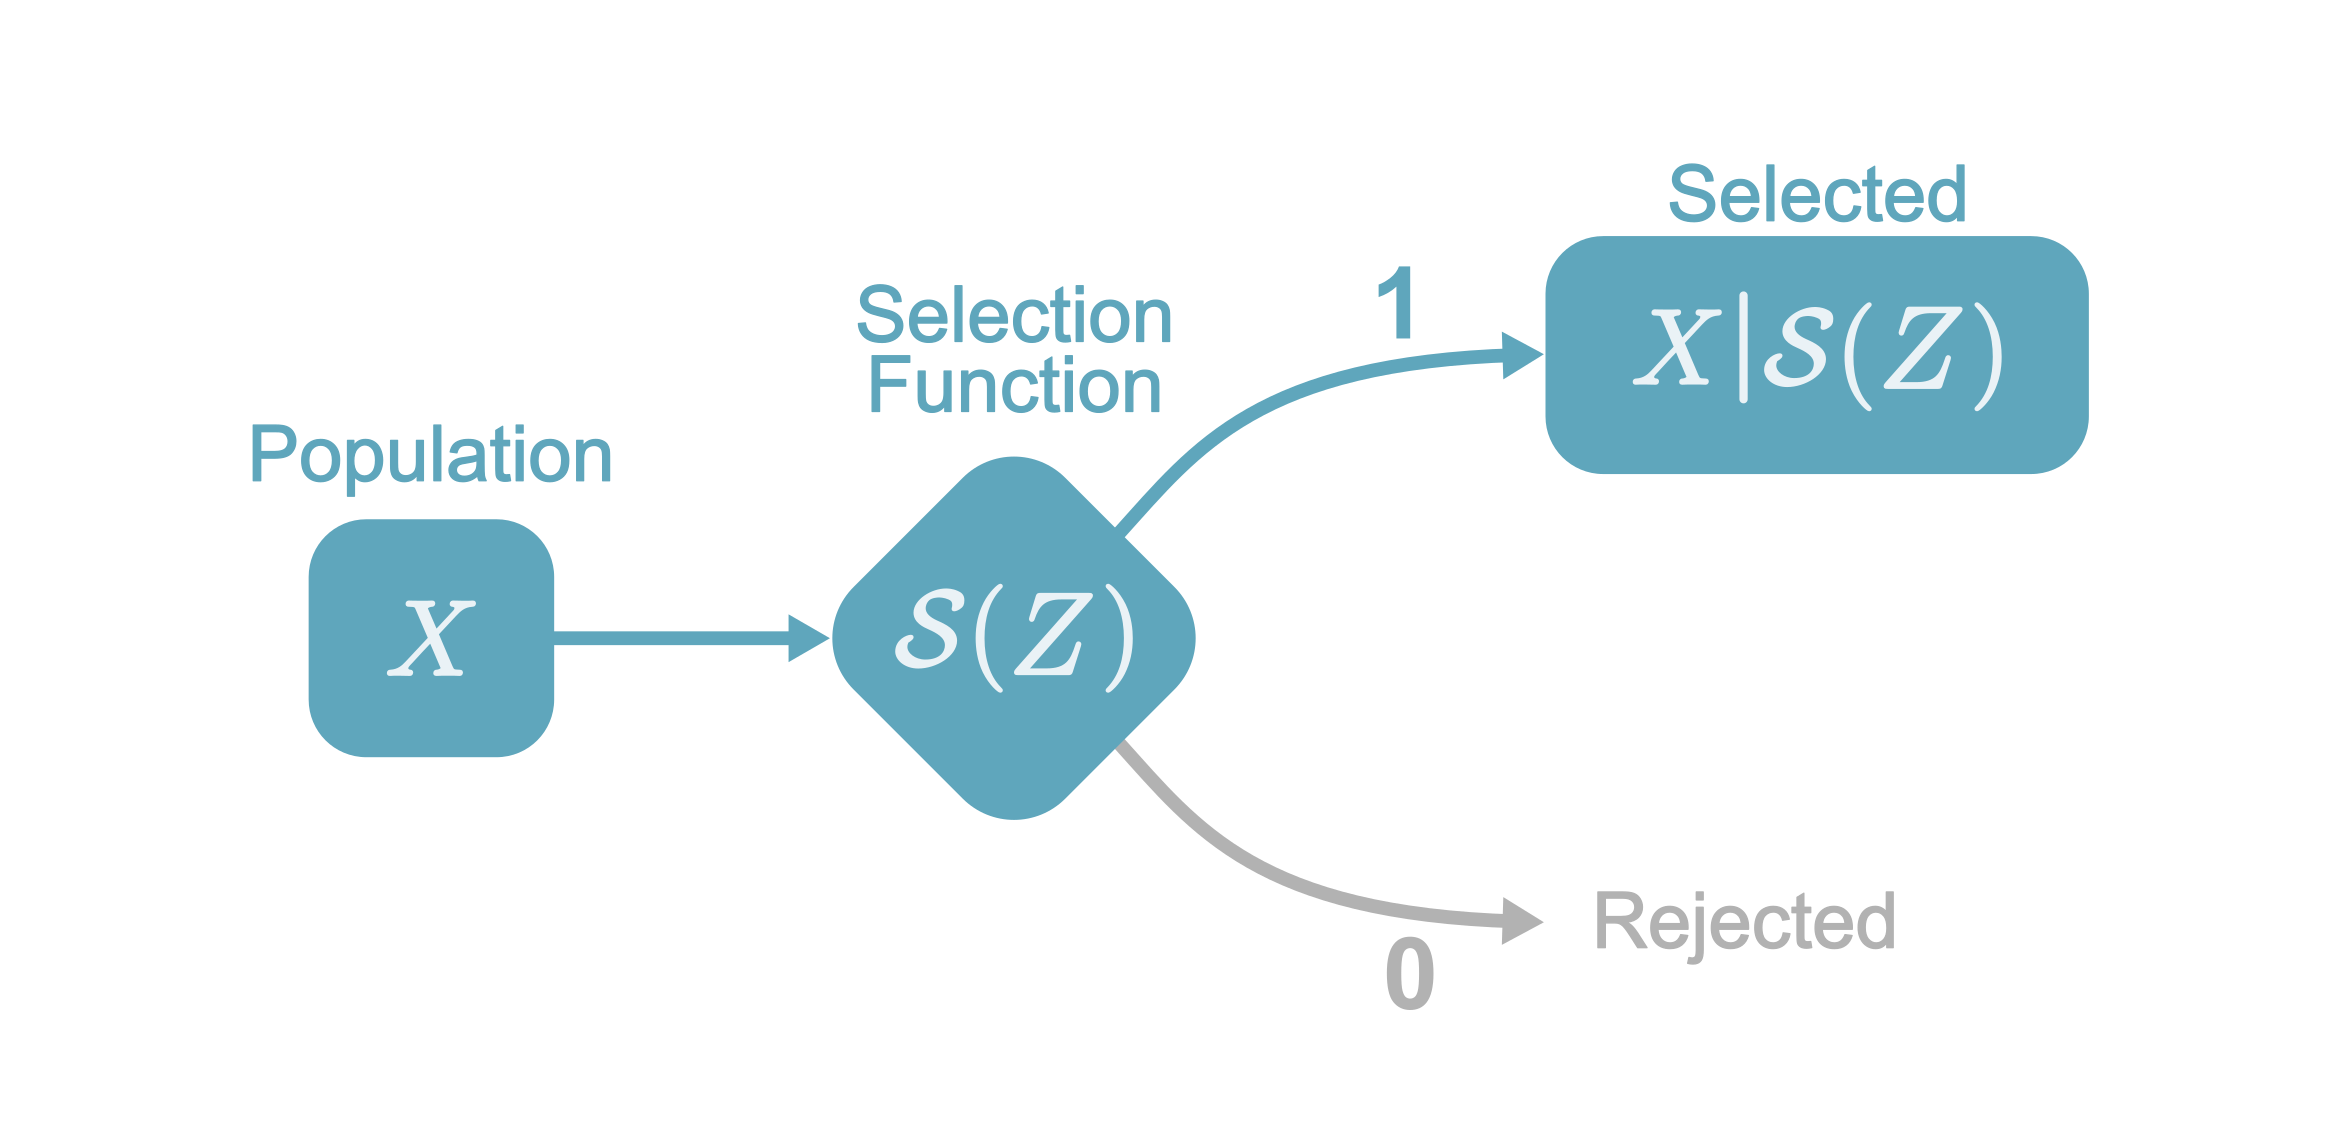
\includegraphics{chapters/10-indirect-selection/figure/indirect_select_diagram.png}

}

\caption{\label{fig-indirect-select-diag}Diagram illustrating the
selection process. The variable, \(X\), is selected based on a function
of itself. Therefore the variable under selection is conditional on the
selection procedure \(X|\mathcal{S}(X)\).}

\end{figure}%

However, selecting on \(Z\) may affect the distribution of \(X\)
depending on the relationship between \(X\) and \(Z\). Particularly, if
we assume normally distributed variables the correlation between \(X\)
and \(Z\) can entirely describe the affect that \(\mathcal{S}(Z)\) has
on the distribution of \(X\). If \(X\) and \(Z\) are independent
(\(\rho_{XZ}=0\)), then selection on \(Z\) would not affect the
distribution of \(X\) such that,

\[
f(X|\mathcal{S}(Z)) = f(X),\;\;\;\; \rho_{XZ}= 0
\]

For example, consider that we select individual's in the top half of
\(Z\) (i.e., above the mean, \(\mu_{Z}\)), such that our selection
function can be defined as,

\[\mathcal{S}(Z) = \begin{cases}1 & \text{if }Z\geq\mu_{Z}\\ 0 & \text{if }Z<\mu_{Z} \end{cases}\]
If the correlation, \(\rho_{XZ}\) is positive, then the distribution of
\(X|\mathcal{S}(Z)\) (i.e., \(X\) given selection on \(Z\)) will have a
higher mean and less variability (see
Figure~\ref{fig-indirect-select-diag})

\begin{figure}[H]

{\centering 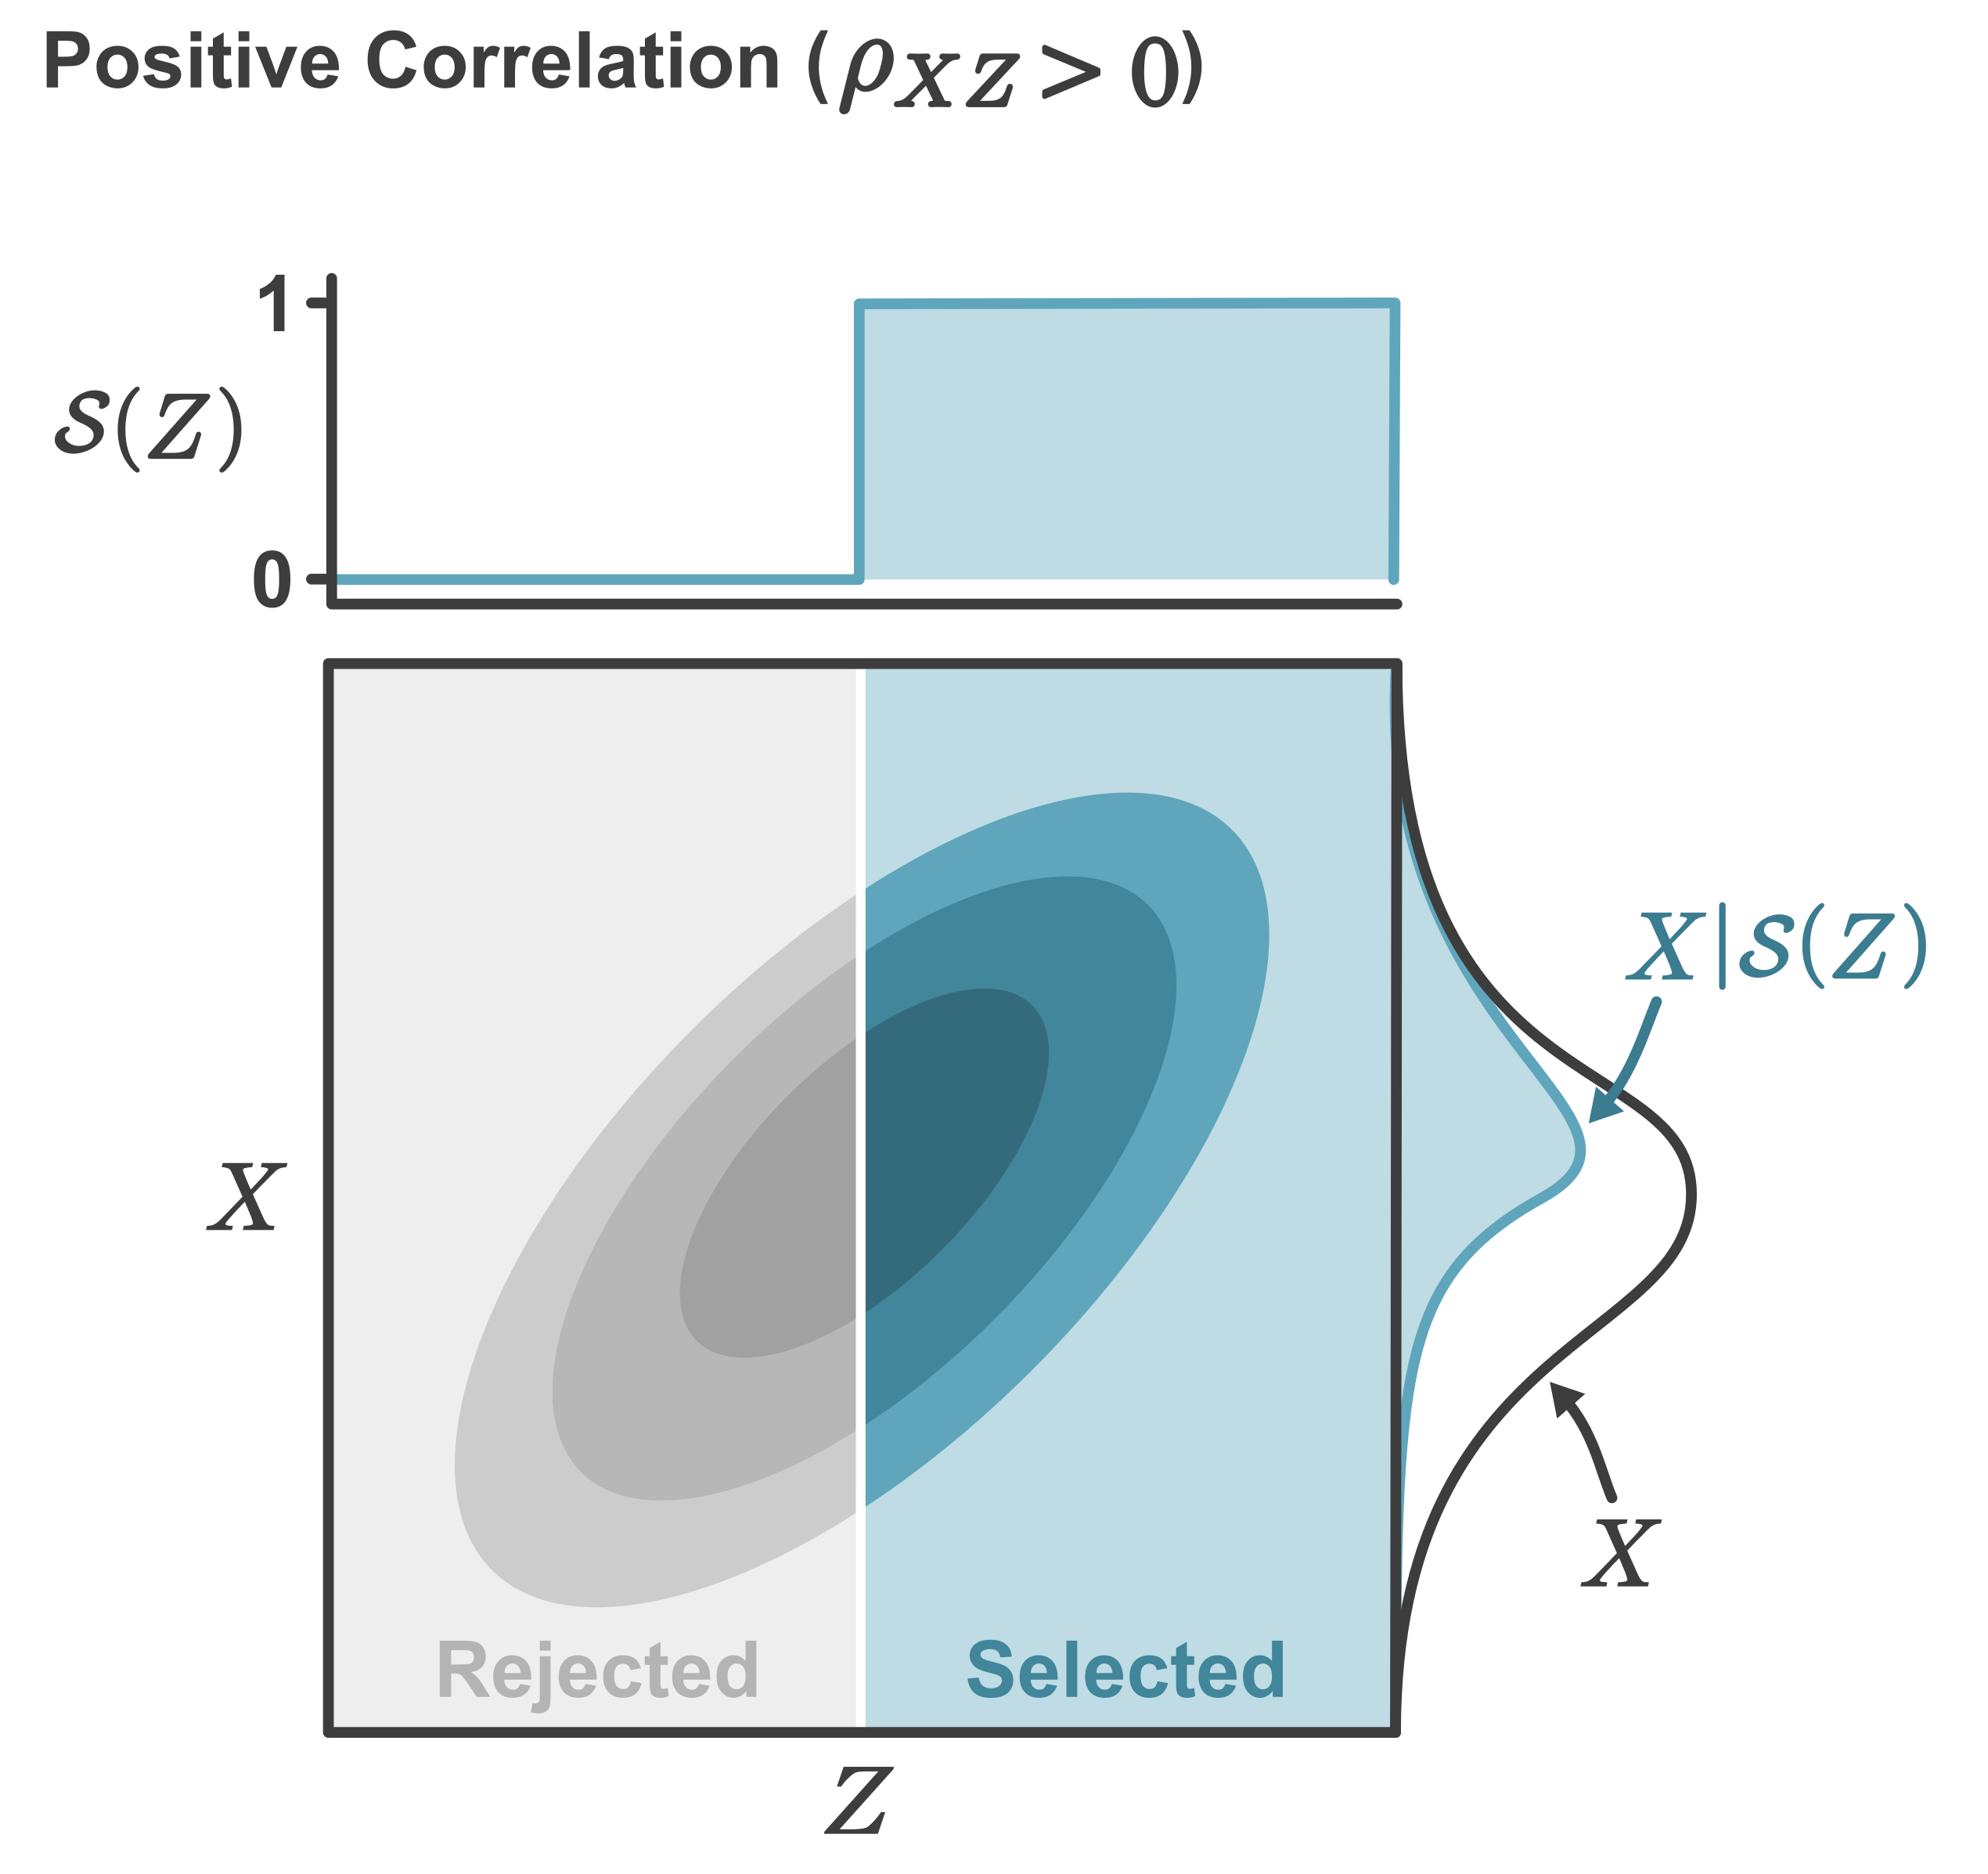
\includegraphics{chapters/10-indirect-selection/figure/selection_function_indirect.png}

}

\caption{Diagram illustrating the impact of selecting on \(Z\) has on
\(X\) given a positive correlation. The selection function on the top of
the plot denotes what values of \(Z\) are selected (i.e.,
\(\mathcal{S}(Z)\)). The distributions on the right indicate the
distribution of \(X\) (in black) and the distribution \(X\) after}

\end{figure}%

If there is no correlation between \(X\) and \(Z\), then the
distribution of \(X|\mathcal{Z}\) would be left unchanged (see
Figure~\ref{fig-indirect-select-diag-no-corr}).

\begin{figure}[H]

\centering{

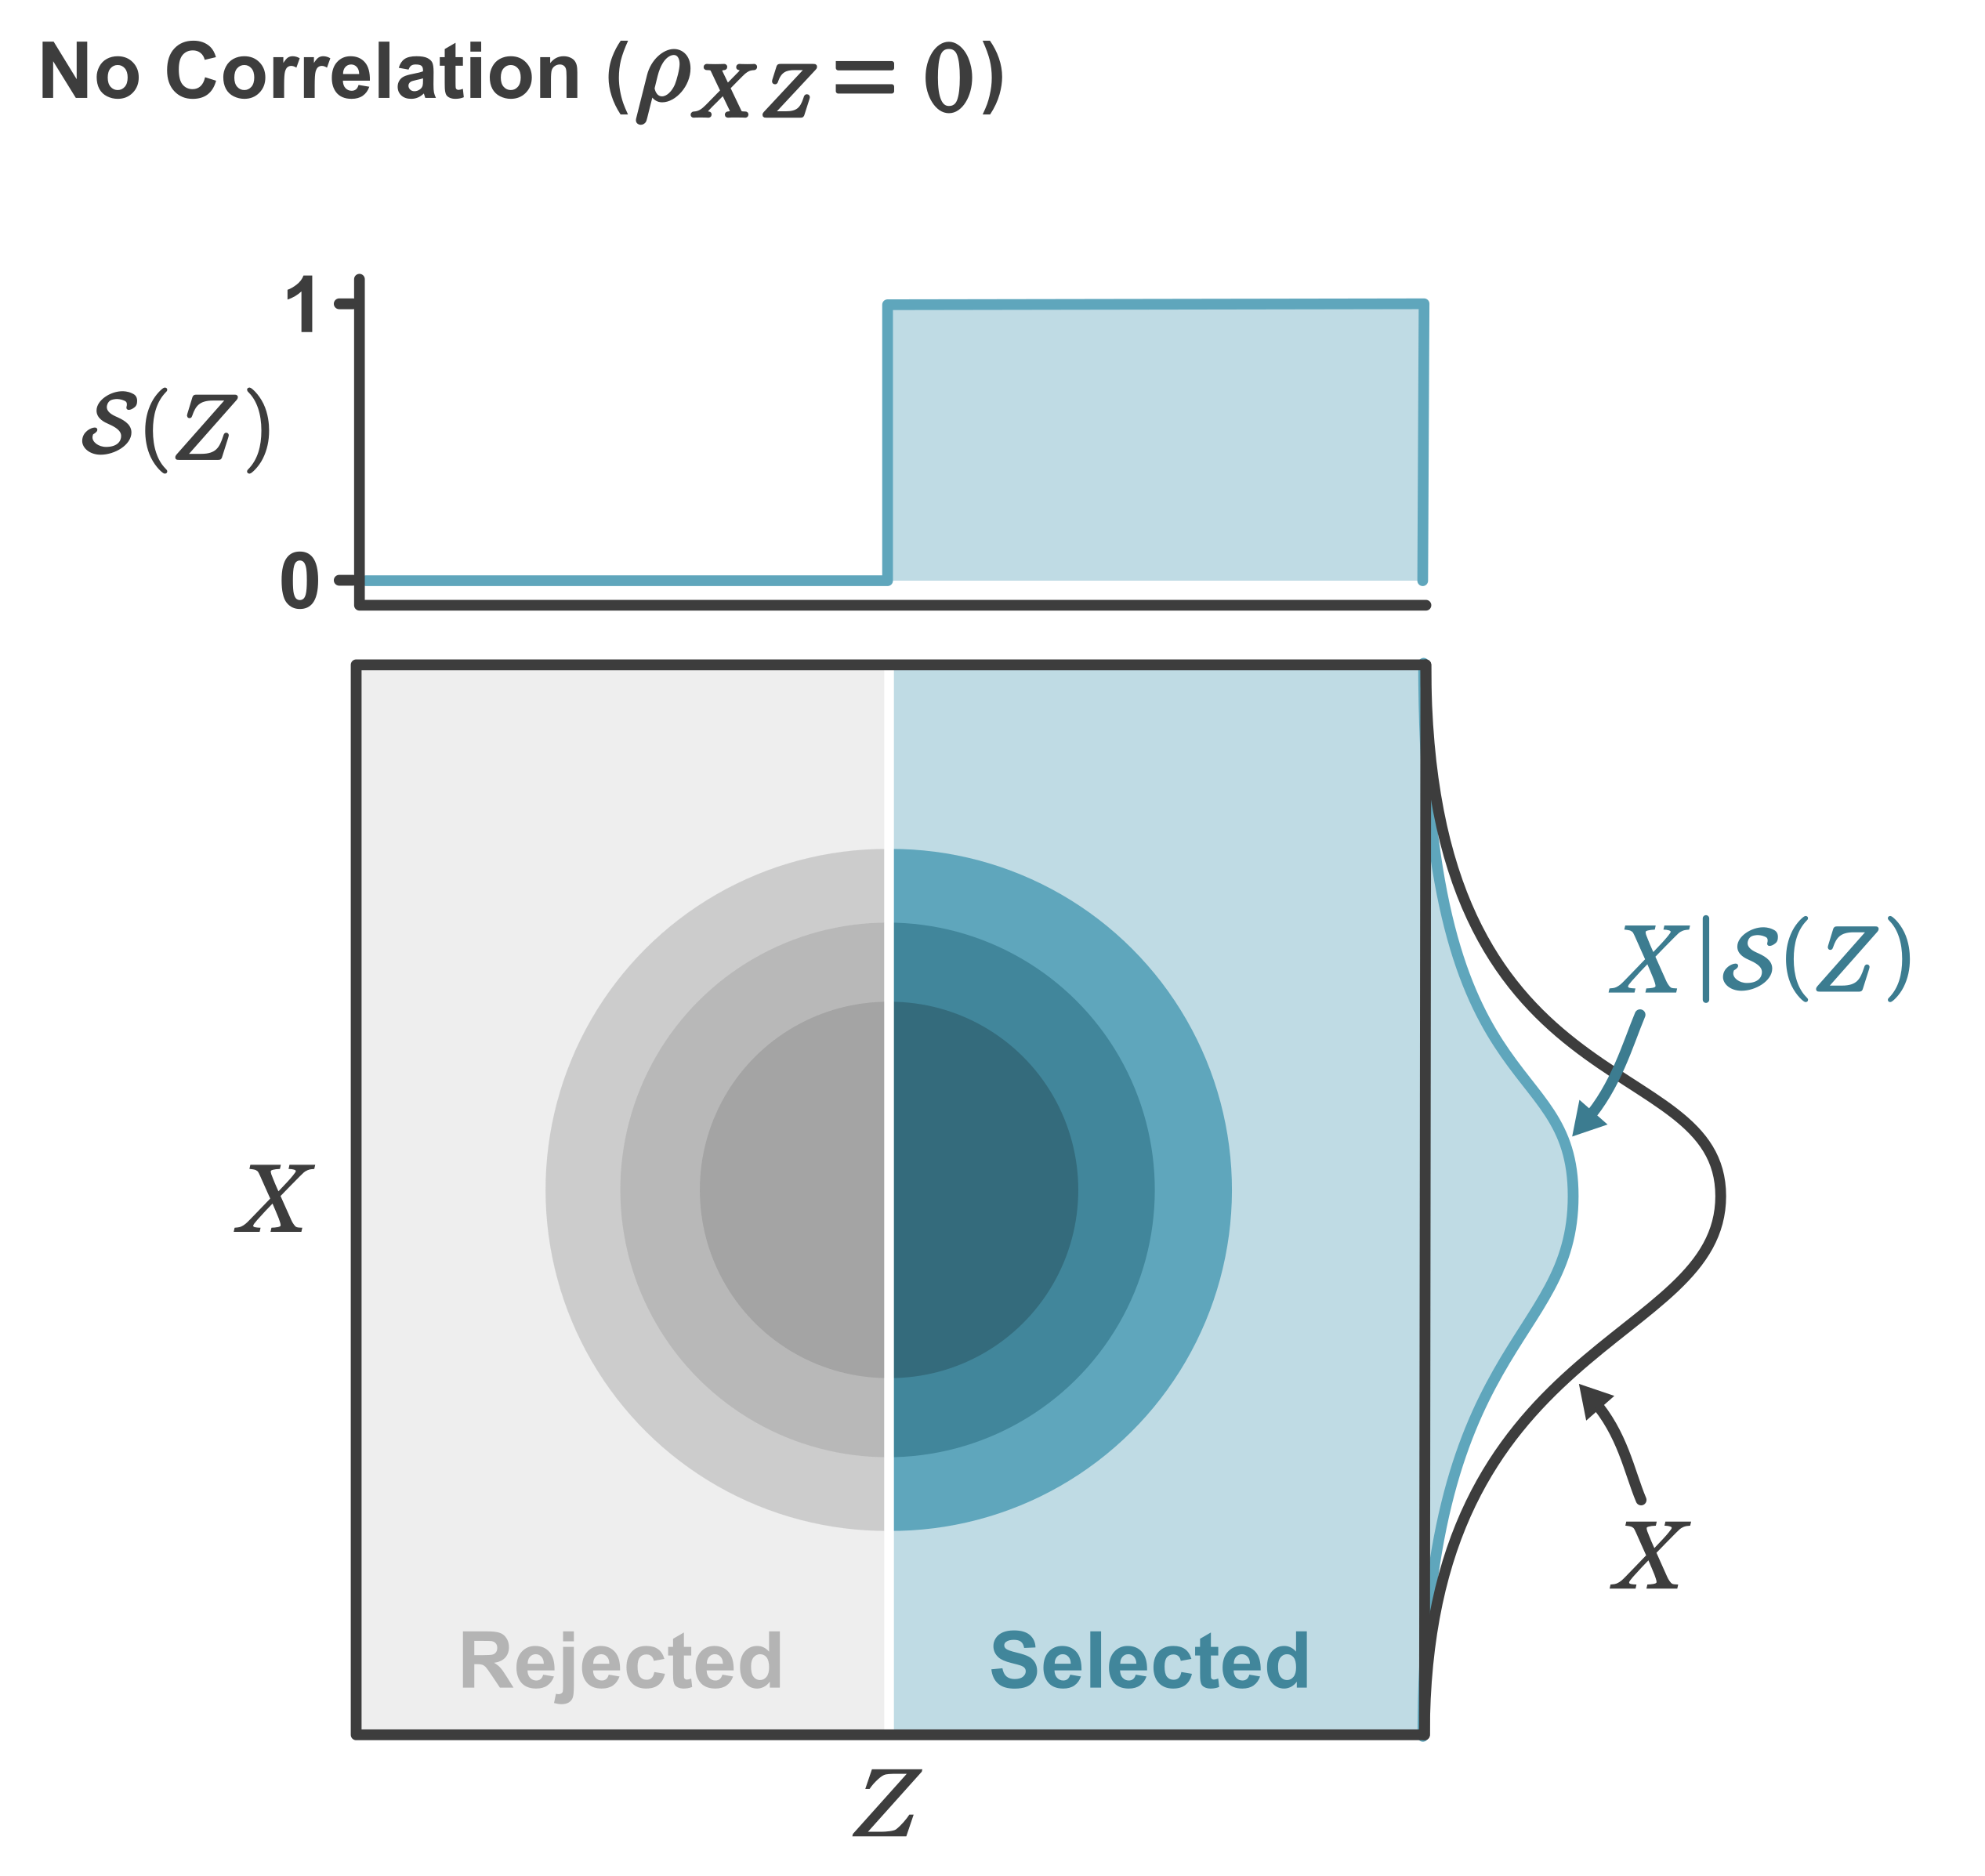
\includegraphics{chapters/10-indirect-selection/figure/selection_function_indirect_no_corr.png}

}

\caption{\label{fig-indirect-select-diag-no-corr}Diagram illustrating
the direct selection function. The variable, \(X\), in the population is
selected based on a function of itself. Therefore the variable under
selection is conditional on the selection procedure
\(X|\mathcal{S}(X)\).}

\end{figure}%

\section{Quantifying Selection-Induced
Restriction/enhancement}\label{quantifying-selection-induced-restrictionenhancement}

The distribution of scores in the target population may exhibit a
greater (or lesser) degree of variability compared to the sample that
has been selected into the study. Therefore the standard deviation of
scores in the target population (\(\sigma_{X}\)) may differ from the
population under selection. (\(\sigma_{X|mathcal{S}(Z)}\)). To index the
difference between the two standard deviations, we can calculate the
\(u\)-ratio Wiernik and Dahlke (2020). The \(u\)-ratio is the ratio
between the standard deviations of the population under selection and
the target population such that (\(\upsilon\) denotes the population
\(u\)-ratio),

\[
\upsilon_X = \frac{\sigma_{X|\mathcal{S}(Z)}}{\sigma_{X}}
\]

The \(u\)-ratio in cases of range \emph{restriction} will exist in the
interval (0--1). Conversely, when the \(u\)-ratio is greater than 1 it
is indicative of range \emph{enhancement}. The target population
standard deviation is often quite difficult to acquire since we do not
usually have access to a random sample from that population. However,
the target population standard deviation can be estimated from a
reference sample that is representative of the target population. This
often comes in the form of standardization samples or norm samples
(obtained from test manuals) if the unrestricted group is the general
population. For example, the distribution full-scale IQ scores derived
from the Wechsler Adult Intelligence Test has a standard deviation of 15
in the US population (Wechsler 2008). We can use this estimate as the
standard deviation for the unrestricted population. Lets say we select a
sample from members of Harvard students, who tend to have higher IQs
than the general population (this is due to the fact that selection
criterion, such as GPA and SAT scores are positively correlated with
IQ). If the standard deviation of IQ in Harvard students is 10, then the
\(u\)-ratio would be,

\[
u_X =  \frac{S_{X|\mathcal{S}(Z)}}{S_X} = \frac{10}{15}= .67
\]

However it is not always the case that an estimate of the unrestricted
standard deviation is readily available. Therefore if the reliability
coefficient from the reference sample and the sample under selection can
be used to estimate the \(u\)-ratio,

\[
u_X = \sqrt{\frac{1-r_{XX'}}{1-r_{XX'|\mathcal{S}(Z)}}}
\]

Where \(r_{XX'|\mathcal{S}(Z)}\) and \(r_{XX'}\) are the reliability
estimates from the sample under selection and the reference (target
population) sample, respectively. In the context of indirect range
restriction, the selection does not occur directly on \(X\) (or \(Y\)),
instead it occurs on a third variable, \(Z\). The affect that selection
on \(Z\) has on \(X\) is dependent on the correlation between them,
\(\rho_{XZ}\). Therefore we can see how the \(u\)-ratio of \(Z\)
(\(u_Z\)) related to the \(u\)-ratio of \(X\),

\[
u_X = \sqrt{\rho_{XZ}^2u_Z^2 -\rho_{XZ}^2 + 1 }
\]

If \(\rho_{XZ}=0\), then you will notice that \(u_X=1\), effectively
having no selection effect on \(X\). Also, notice that a correlation of
\(\rho_{XZ}=1\) will return \(u_X=u_Z\), indicating that selecting on
\(Z\) would affect the variation of \(Z\) similarly to the variation in
\(X\). This relationship between \(u_X\), \(u_Z\), and \(\rho_{XZ}\) can
be visualized in Figure~\ref{fig-ux-uz}

\begin{figure}[H]

\centering{

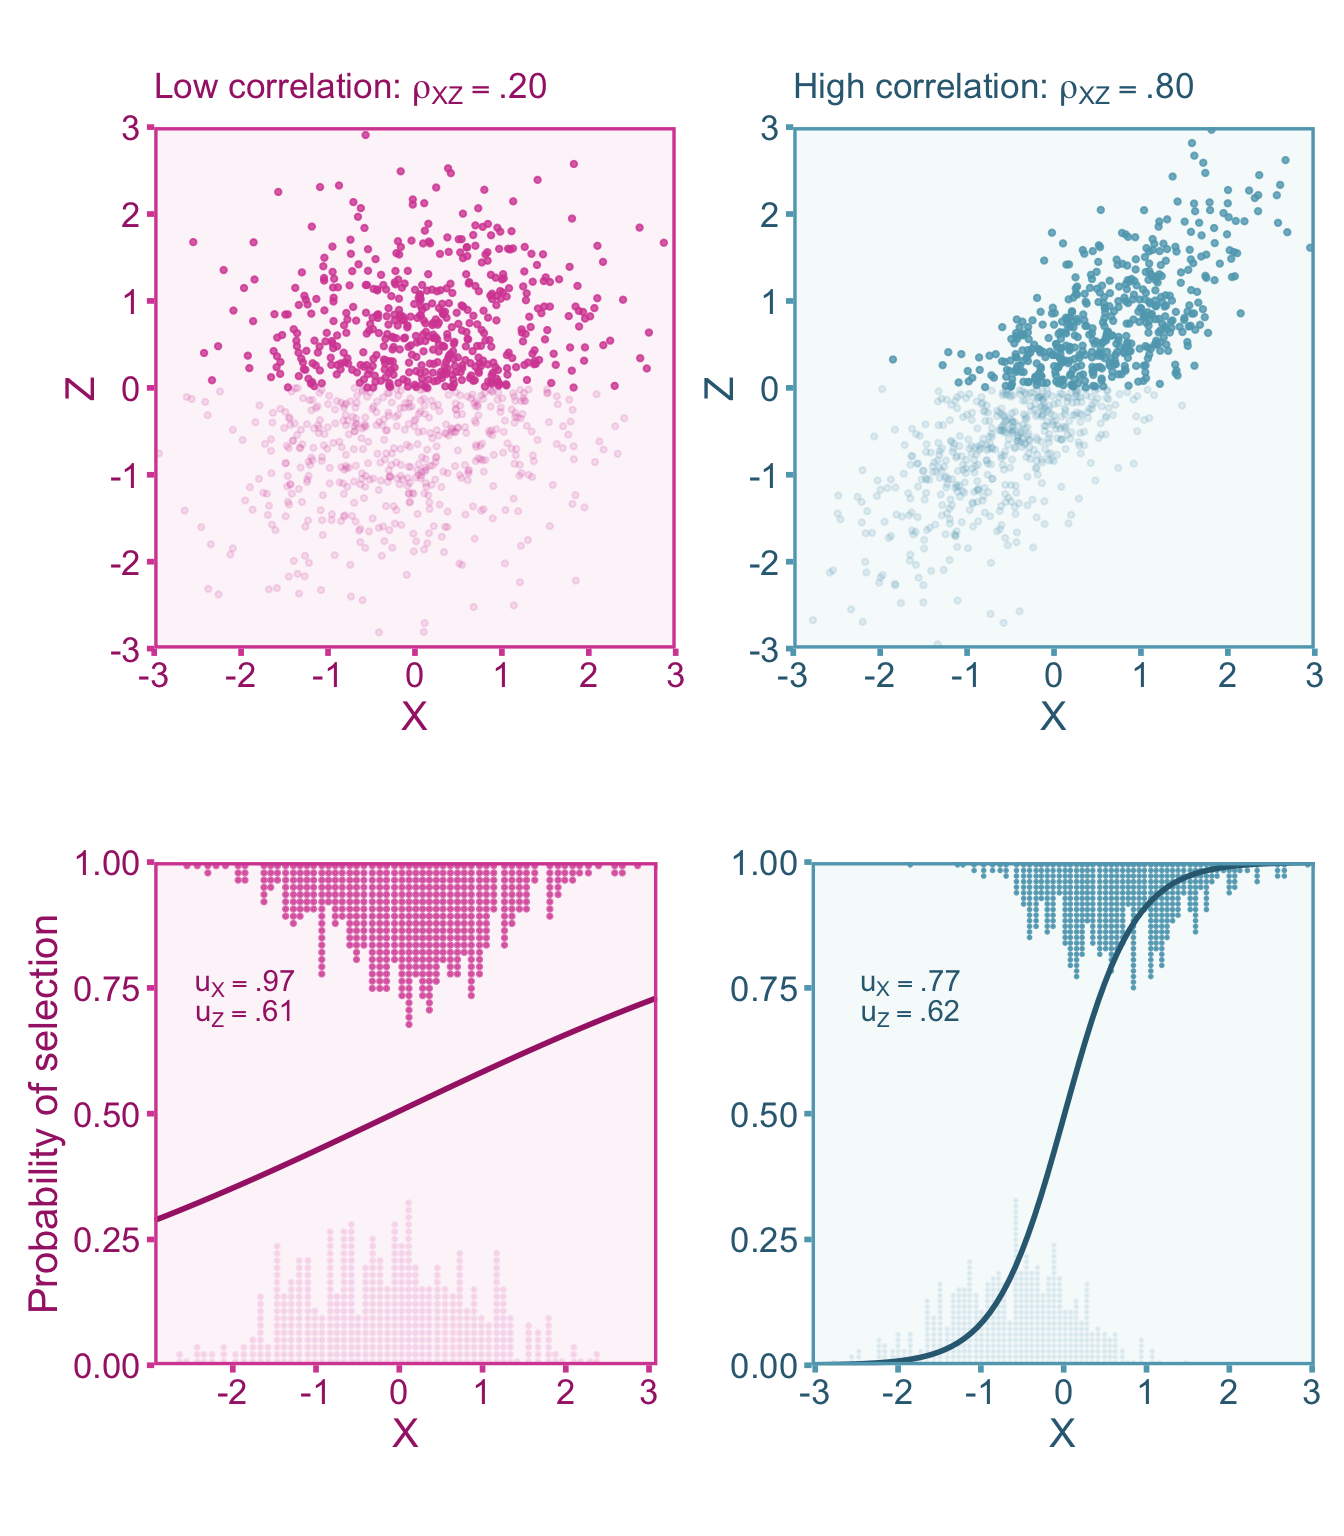
\includegraphics{chapters/10-indirect-selection/10-indirect-selection_files/figure-pdf/fig-ux-uz-1.pdf}

}

\caption{\label{fig-ux-uz}The impact of the association between \(X\)
and \(Z\). The data consists of \(N=1,000\) simulated observations,
where the red plots show a low correlation case (\(\rho_{XZ}=.20\)) and
the blue plots show a high correlation case (\(\rho_{XZ}=.80\)). The top
plots show the relationship between \(X\) and \(Z\) with the darker
points indicating individuals that have been selected into the sample.
The bottom plots shows the probability of selection into the sample as a
function of X. The dark distribution on the top of the plot show the
distribution of individuals in the selected sample. Notice that the
distribution of the selected individual's in the high correlation case
is a narrower distribution than the low correlation case.}

\end{figure}%

\section{Correcting Correlations for Indirect Range
Restriction}\label{correcting-correlations-for-indirect-range-restriction}

\subsection{Defining our Target
Quantity}\label{defining-our-target-quantity-6}

We want to estimate the population correlation of the true scores of the
independent variable (\(T\)) and dependent variable (\(U\)). We can
denote this correlation as \(\rho_{TU}\). Within a study sample that
suffers from indirect selection (and sampling error), the study
correlation is under selection (\(r_{xy_S}\)) will be biased relative to
our target quantity, \(\rho_{xy}\). This bias is captured by an artifact
attenuation/inflation factor, \(a\), such that,

\[
r_{XY} = a \rho_{XY|\mathcal{S}(Z)} + e 
\]

Therefore an unbiased estimate of the true score target population
correlation can be estimated by dividing the observed score correlation
under selection by an estimate of \(a\),

\[
r_{TU} = \frac{ r_{XY|\mathcal{S}(Z)} }{ \hat{a}}.
\]

\subsection{Artifact Correction for
Correlations}\label{artifact-correction-for-correlations}

\subsubsection*{The Univariate Case}\label{the-univariate-case-2}
\addcontentsline{toc}{subsubsection}{The Univariate Case}

Range restriction (or enhancement) in either the independent or
dependent variable will induce bias into the correlation coefficient.
Let us consider a case where we select individuals based on meeting some
criterion of some third variable, \(Z\), such that \(\mathcal{S}(Z)\).
In the univariate case, we assume that selection on \(Z\) only directly
affects restriction/enhancement in \(X\) while any
restriction/enhancement in \(Y\) is mediated by the effect on \(X\) (see
Figure~\ref{fig-corr-model-uni}).

Now consider a study where we want to calculate correlation in the
target population between an independent variable, \(X\), and a
dependent variable, \(Y\). However, the individual's are selected
whether they are above the mean of \(Z\) (Mean = 0). We can thus define
the selection function such that,

\[
\mathcal{S}(Z) = \begin{cases} 1 & \text{if } Z \geq 0 \\ 0 & \text{if } Z < 0 \end{cases}
\]

In the following examples, we will simulate a correlation of
\(\rho_{XZ}=.80\).

\begin{figure}[H]

\centering{

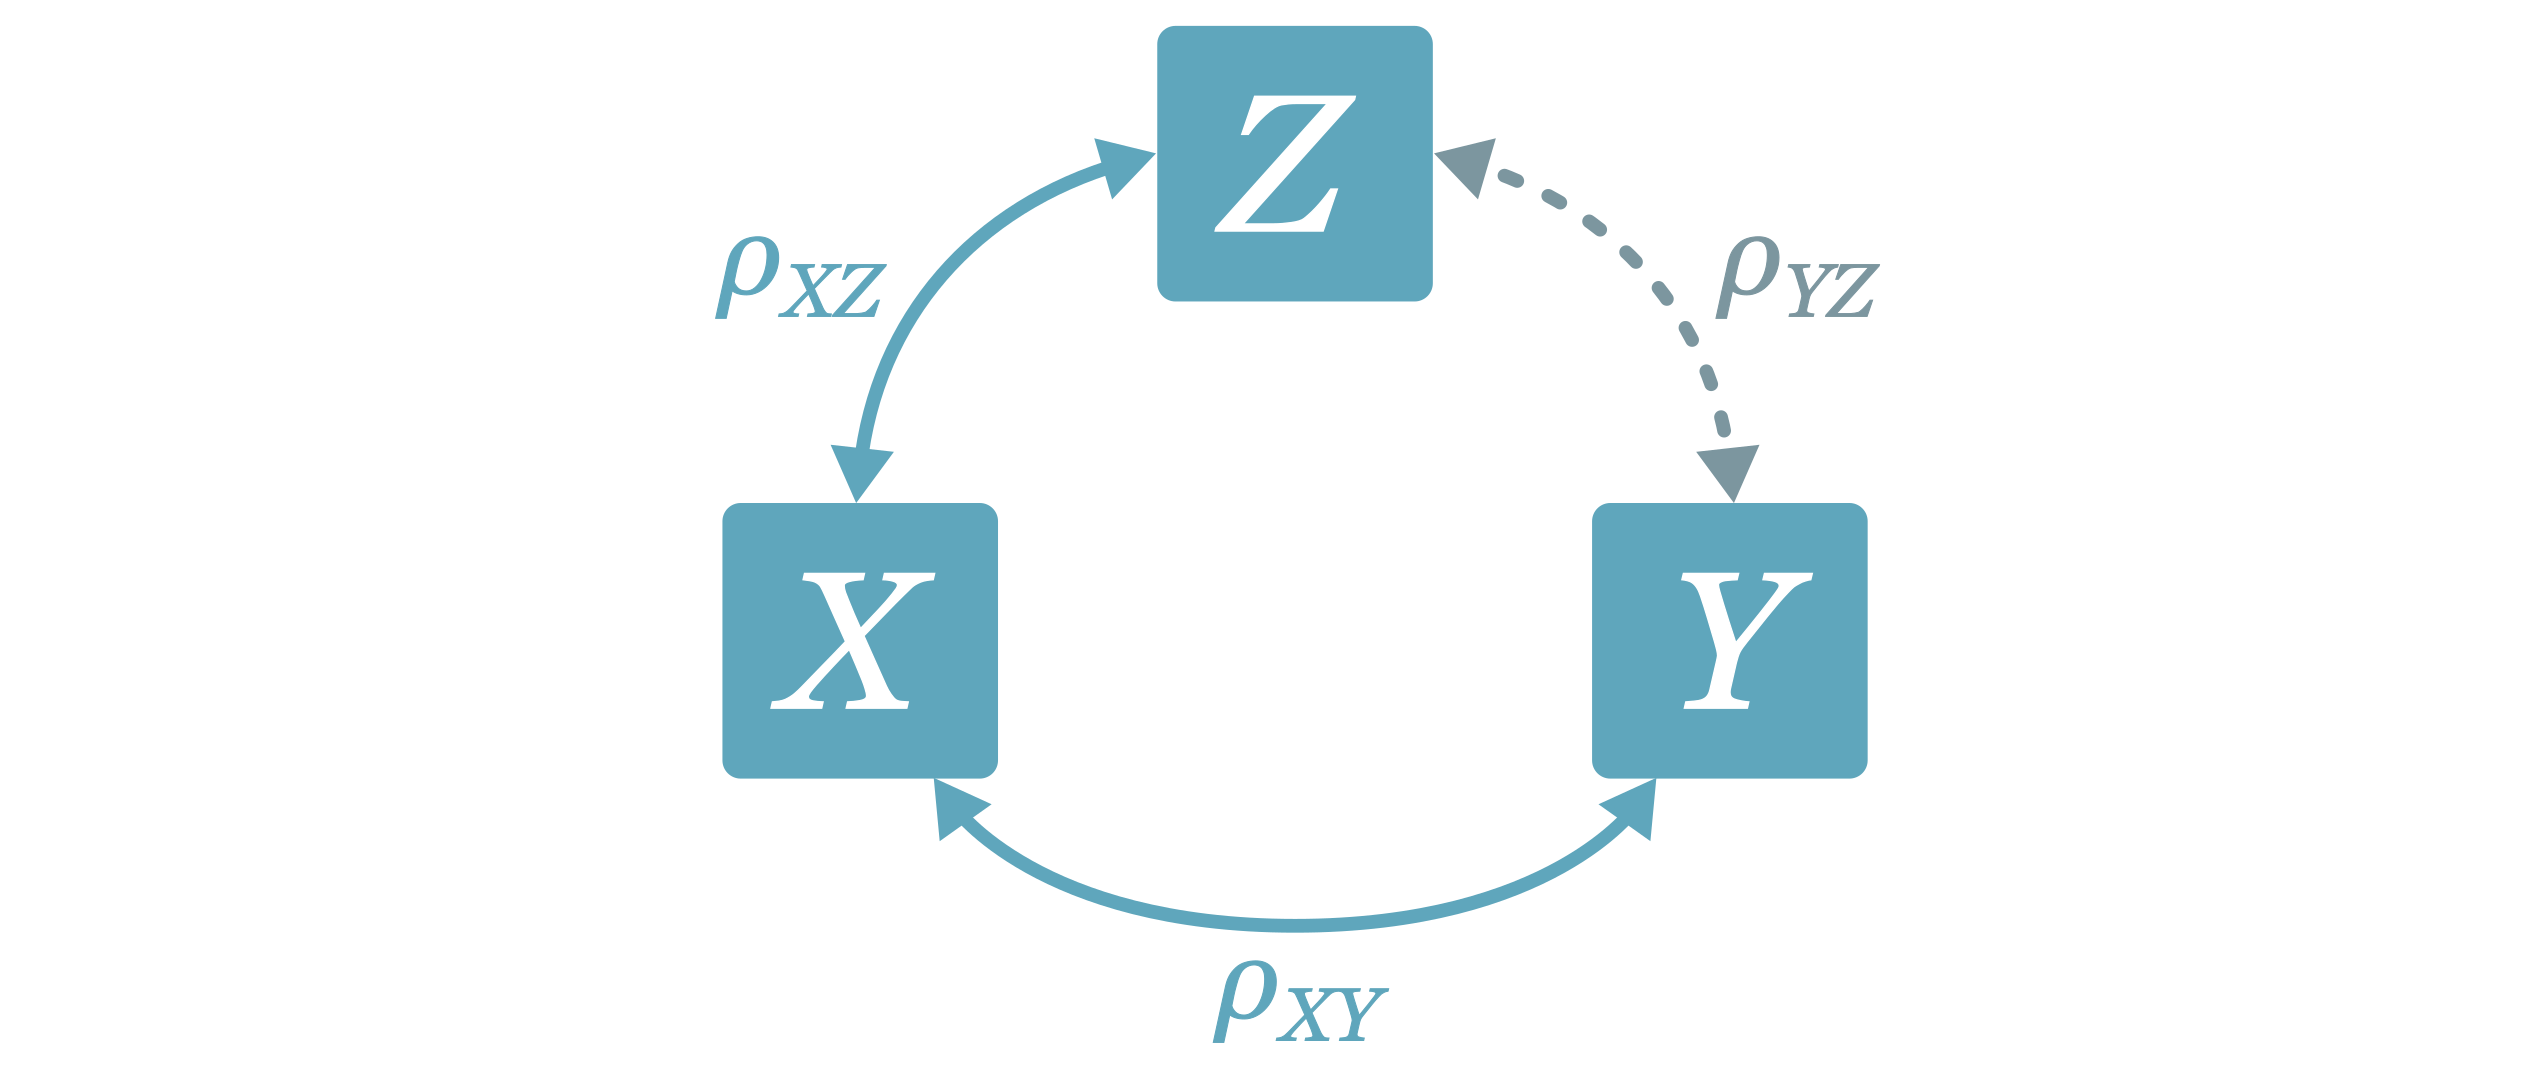
\includegraphics{chapters/10-indirect-selection/figure/indirect_select_corr_model_uni.png}

}

\caption{\label{fig-corr-model-uni}The assumed correlation structure of
univariate indirect selection. The correlation between \(Z\) and \(Y\)
is completely mediated by \(X\) (i.e., the partial correlation between
\(Y\) and \(Z\), controlling for \(X\) is zero such that,
\(\rho_{YZ.X}=0\)).}

\end{figure}%

Figure~\ref{fig-uvirr} shows a \(u\)-ratio of about \(u_X=0.75\) in the
independent variable. We see that the sample correlation in the
restricted scores (\(r_{XY|\mathcal{S}(Z)}=.42\)) is attenuated relative
to the unrestricted correlation (\(r_{XY}=.50\)).

\begin{figure}[H]

\centering{

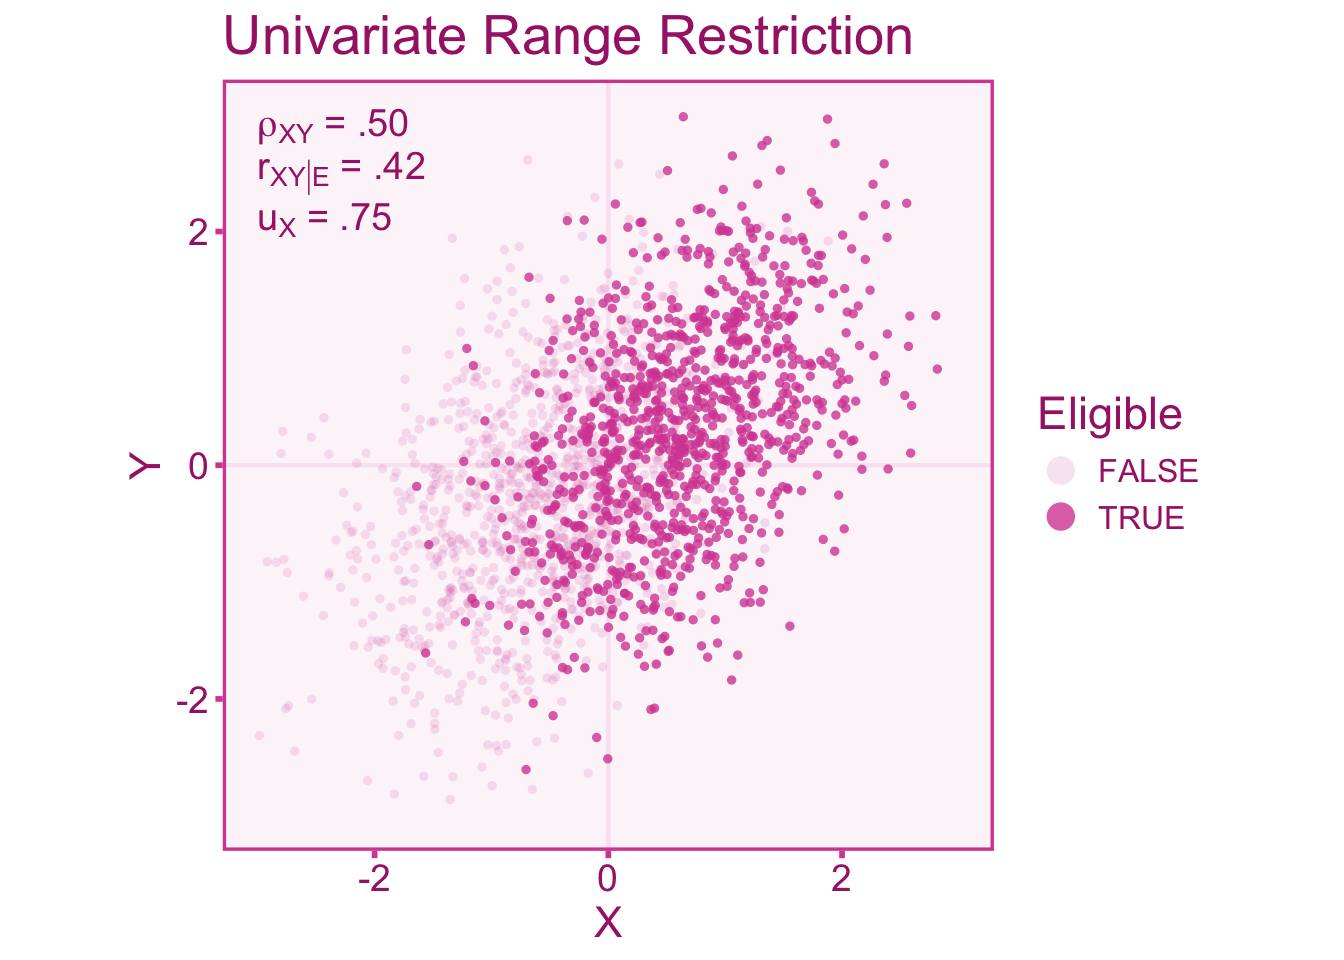
\includegraphics{chapters/10-indirect-selection/10-indirect-selection_files/figure-pdf/fig-uvirr-1.pdf}

}

\caption{\label{fig-uvirr}Scatterplot showing a correlation between
\(X\) and \(Y\) under univariate indirect range restriction. Dark red
dots indicate the selected sample and the transparent dots indicate the
rejected sample.}

\end{figure}%

We can also visualize what happens to the correlation when the range is
enhanced. Enhancement can be accomplished by selecting individuals at
the ends of the distribution (Taylor and Griess 1976). For indirect
selection, individuals are selected at the ends of the distribution of
\(Z\) such that the selection function can be defined as,

\[
\mathcal{S}(Z) = \begin{cases} 1 & \text{if } Z \leq -1 \text{ or } Z \geq 1 \\ 0 & \text{if } Z < -1 \text{ or } Z >1 \end{cases}
\]

In Figure~\ref{fig-uvire}, we see an opposite effect on the correlation,
that is, an inflation of the correlation rather than an attenuation like
we see under range restriction. The scenario below has a \(u\)-ratio of
about \(u_X=1.32\) in the independent variable.

\begin{figure}[H]

\centering{

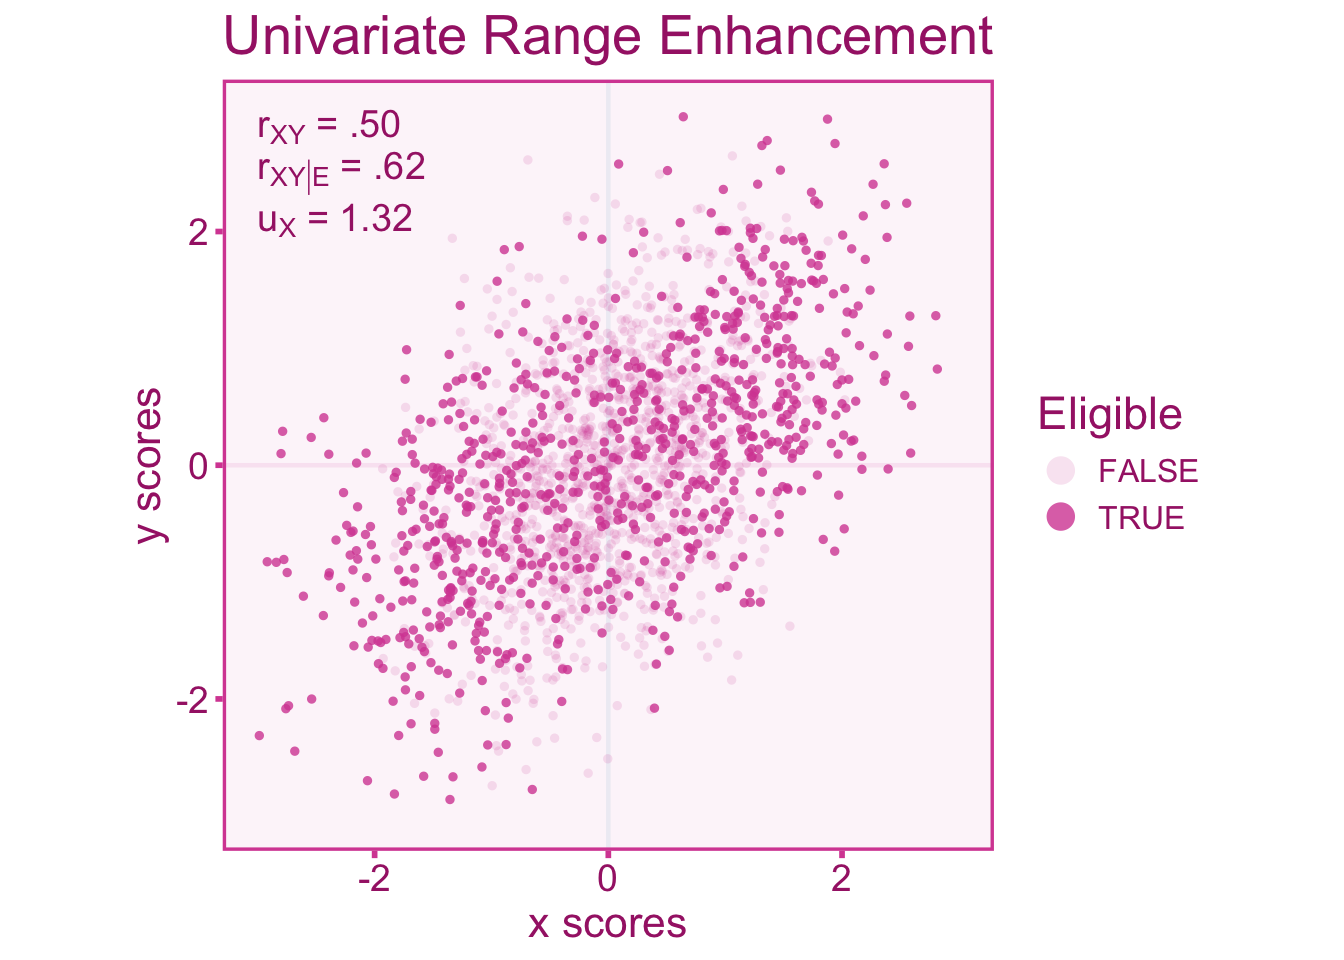
\includegraphics{chapters/10-indirect-selection/10-indirect-selection_files/figure-pdf/fig-uvire-1.pdf}

}

\caption{\label{fig-uvire}Scatterplot showing a correlation between
\(X\) and \(Y\) under univariate indirect range enhancement. Dark red
dots indicate the selected sample and the transparent dots indicate the
rejected sample.}

\end{figure}%

In summary, if \(u_X>1\) (i.e., \(S_{X|\mathcal{S}(Z)}>S_{X}\)) the
observed correlation is inflated relative to the correlation in the
target population. Whereas the correlation is attenuated when \(u_X<1\)
(i.e., \(S_{X|\mathcal{S}(Z)}<S_{X}\), Sackett and Yang 2000). An
estimate of the attenuation/inflation factor, \(\hat{a}\), can account
for the bias in the observed correlation induced by range
restriction/enhancement (equation 5, Le and Schmidt 2006).

\[
\hat{a} = \sqrt{r_{XY|\mathcal{S}(Z)}^2 + u_{X}^2 (1- r_{XY|\mathcal{S}(Z)}^2)  }
\] Using the estimated attenuation/inflation factor, we can correct the
observed correlation for bias induced by indirect selection

\begin{equation}\phantomsection\label{eq-univariate}{
r_{XY} = \frac{r_{XY|\mathcal{S}(Z)}}{\hat{a}} = \frac{r_{XY|\mathcal{S}(Z)}}{\sqrt{r_{XY|\mathcal{S}(Z)}^2 + u_{X}^2 (1- r_{XY|\mathcal{S}(Z)}^2)  }}
}\end{equation}

If we wants to correct for range restriction/enhancement \emph{and}
measurement error, we can incorporate the reliability coefficients
(under selection) of \(X\) (\(r_{XX'|\mathcal{S}(Z)}\)) and \(Y\)
(\(r_{YY'|\mathcal{S}(Z)}\)) into the formula for \(\hat{a}\),

\[
\hat{a} = \sqrt{r_{XY|\mathcal{S}(Z)}^2 + \frac{u_{X}^2 r_{XX'|\mathcal{S}(Z)}\left(r_{XX'|\mathcal{S}(Z)}r_{YY'|\mathcal{S}(Z)} - r_{XY|\mathcal{S}(Z)}^2\right) }{1 - u_{X}^2 \left(1-r_{XX'|\mathcal{S}(Z)}\right)} }
\]

Now correcting the observed correlation with this modified estimate of
\(a\) to correct the observed correlation will yield the true score
correlation in the target population,

\[
r_{TU}=\frac{r_{XY|\mathcal{S}(Z)}}{\hat{a}} = \frac{r_{XY|\mathcal{S}(Z)}}{\sqrt{r_{XY|\mathcal{S}(Z)}^2 + \frac{u_{X}^2 r_{XX'|\mathcal{S}(Z)}\left(r_{XX'|\mathcal{S}(Z)}r_{YY'|\mathcal{S}(Z)} - r_{XY|\mathcal{S}(Z)}^2\right) }{1 - u_{X}^2 \left(1-r_{XX'|\mathcal{S}(Z)}\right)} }}
\]

If the reliability coefficients come from the target population and do
not suffer selection effects, we can estimate the reliability under
selection using the following formulas (equation 11 and 12 Le and
Schmidt 2006):

\begin{equation}\phantomsection\label{eq-rel-x}{
r_{XX'|\mathcal{S}(Z)} = 1-\frac{1-r_{XX'}}{u_X^2}
}\end{equation}

\begin{equation}\phantomsection\label{eq-rel-y}{
r_{YY'|\mathcal{S}(Z)} = 1-\frac{1-r_{YY'}}{u_Y^2}
}\end{equation}

We now need to adjust the standard error for the corrected correlation
coefficient. To do this, we can either divide the observed standard
error by the attenuation/inflation factor (or equivalently, the observed
correlation divided by the corrected correlation),

\[
se(r_{TU}) = \frac{se\left(r_{XY|\mathcal{S}(Z)}\right)}{\hat{a}}= \frac{se\left(r_{XY|\mathcal{S}(Z)}\right)}{\left[\frac{r_{XY|\mathcal{S}(Z)}}{r_{TU}}\right]}.
\]

\begin{tcolorbox}[enhanced jigsaw, opacityback=0, coltitle=black, toprule=.15mm, colframe=quarto-callout-note-color-frame, bottomtitle=1mm, rightrule=.15mm, colbacktitle=quarto-callout-note-color!10!white, left=2mm, bottomrule=.15mm, breakable, title={Applied Example in R}, colback=white, opacitybacktitle=0.6, titlerule=0mm, arc=.35mm, leftrule=.75mm, toptitle=1mm]

Let's say a university admits students based on some criterion upon a
composite of multiple measures of performance (\(Z\)). One of those
measures is a standardized test (\(X\)). A researcher then wants to see
how test performance predicts stress (\(Y\)) in college. Since test
performance is correlated with the composite used in the college
admissions process, it is likely that we will observe substantial range
restriction in the college sample. To index this restriction in range,
we calculate the \(u\)-ratio of test scores as \(u_{X}=0.70\) (relative
to the total pool of applicants). We also want to correct for
measurement error in test performance and the self-report questionnaire
we use to measure stress, therefore we obtain reliability estimates
within our sample of \(r_{XX'|\mathcal{S}(Z)}=.90\) and
\(r_{XX'|\mathcal{S}(Z)}=.80\), respectively. The researcher then
conducts the study and finds a sample correlation of
\(r_{XY|\mathcal{S}(Z)}=.25\), but he wants to know that true score
correlation.

In R, we can correct the correlation by using the \texttt{correct\_r}
function in the \texttt{psychmeta} package (Dahlke and Wiernik 2019).
The \texttt{correction\ =\ \textquotesingle{}uvirr\_x\textquotesingle{}}

\begin{Shaded}
\begin{Highlighting}[]
\FunctionTok{library}\NormalTok{(psychmeta)}

\FunctionTok{correct\_r}\NormalTok{(}\AttributeTok{correction =} \StringTok{\textquotesingle{}uvirr\_x\textquotesingle{}}\NormalTok{,}
          \AttributeTok{rxyi =}\NormalTok{ .}\DecValTok{25}\NormalTok{,  }\CommentTok{\# restricted correlation}
          \AttributeTok{rxx =}\NormalTok{ .}\DecValTok{90}\NormalTok{,  }\CommentTok{\# reliability of test scores}
          \AttributeTok{ryy =}\NormalTok{ .}\DecValTok{80}\NormalTok{,  }\CommentTok{\# reliability of stress}
          \AttributeTok{ux =}\NormalTok{ .}\DecValTok{70}\NormalTok{,   }\CommentTok{\# u ratio of SAT scores}
          \AttributeTok{n =} \DecValTok{100}\NormalTok{)    }\CommentTok{\# sample size}
\end{Highlighting}
\end{Shaded}

\begin{verbatim}
Correlations Corrected for Measurement Error and Univariate Indirect Range Restriction:
---------------------------------------------------------------------------------------
  value CI_LL_95 CI_UL_95   n n_effective
1 0.412   0.0973    0.648 100        33.8
\end{verbatim}

The true score correlation in the target population is estimated to be
\(r_{TU} = .41\, [.10,\, .65]\).

\end{tcolorbox}

\subsubsection*{The Bivariate Case}\label{the-bivariate-case-2}
\addcontentsline{toc}{subsubsection}{The Bivariate Case}

Bivariate indirect range restriction/enhancement occurs when the
selection variable has independent relationships with both the
independent and dependent variable. Like we did for the univariate case,
let's visualize the correlation between independent (\(X\)) and
dependent (\(Y\)) variables under range restriction by only selecting
individuals above a score of -0.50 in our selector variable, \(Z\).
Therefore the selection function can be defined as,

\[
\mathcal{S}(Z)=\begin{cases} 1 &\text{ if } Z \geq-.50 \\  0 &\text{ if } Z <-.50  \end{cases}
\]

We will also fix the correlations between the selector and independent
variable (\(\rho_{XZ}\)), as well as the selector and dependent variable
(\(\rho_{YZ}\)) to be .80. Unlike the univariate case, in the bivariate
case \(X\) \emph{and} \(Y\) have direct relationships with \(Z\) (see
Figure~\ref{fig-corr-model-biv}).

\begin{figure}[H]

\centering{

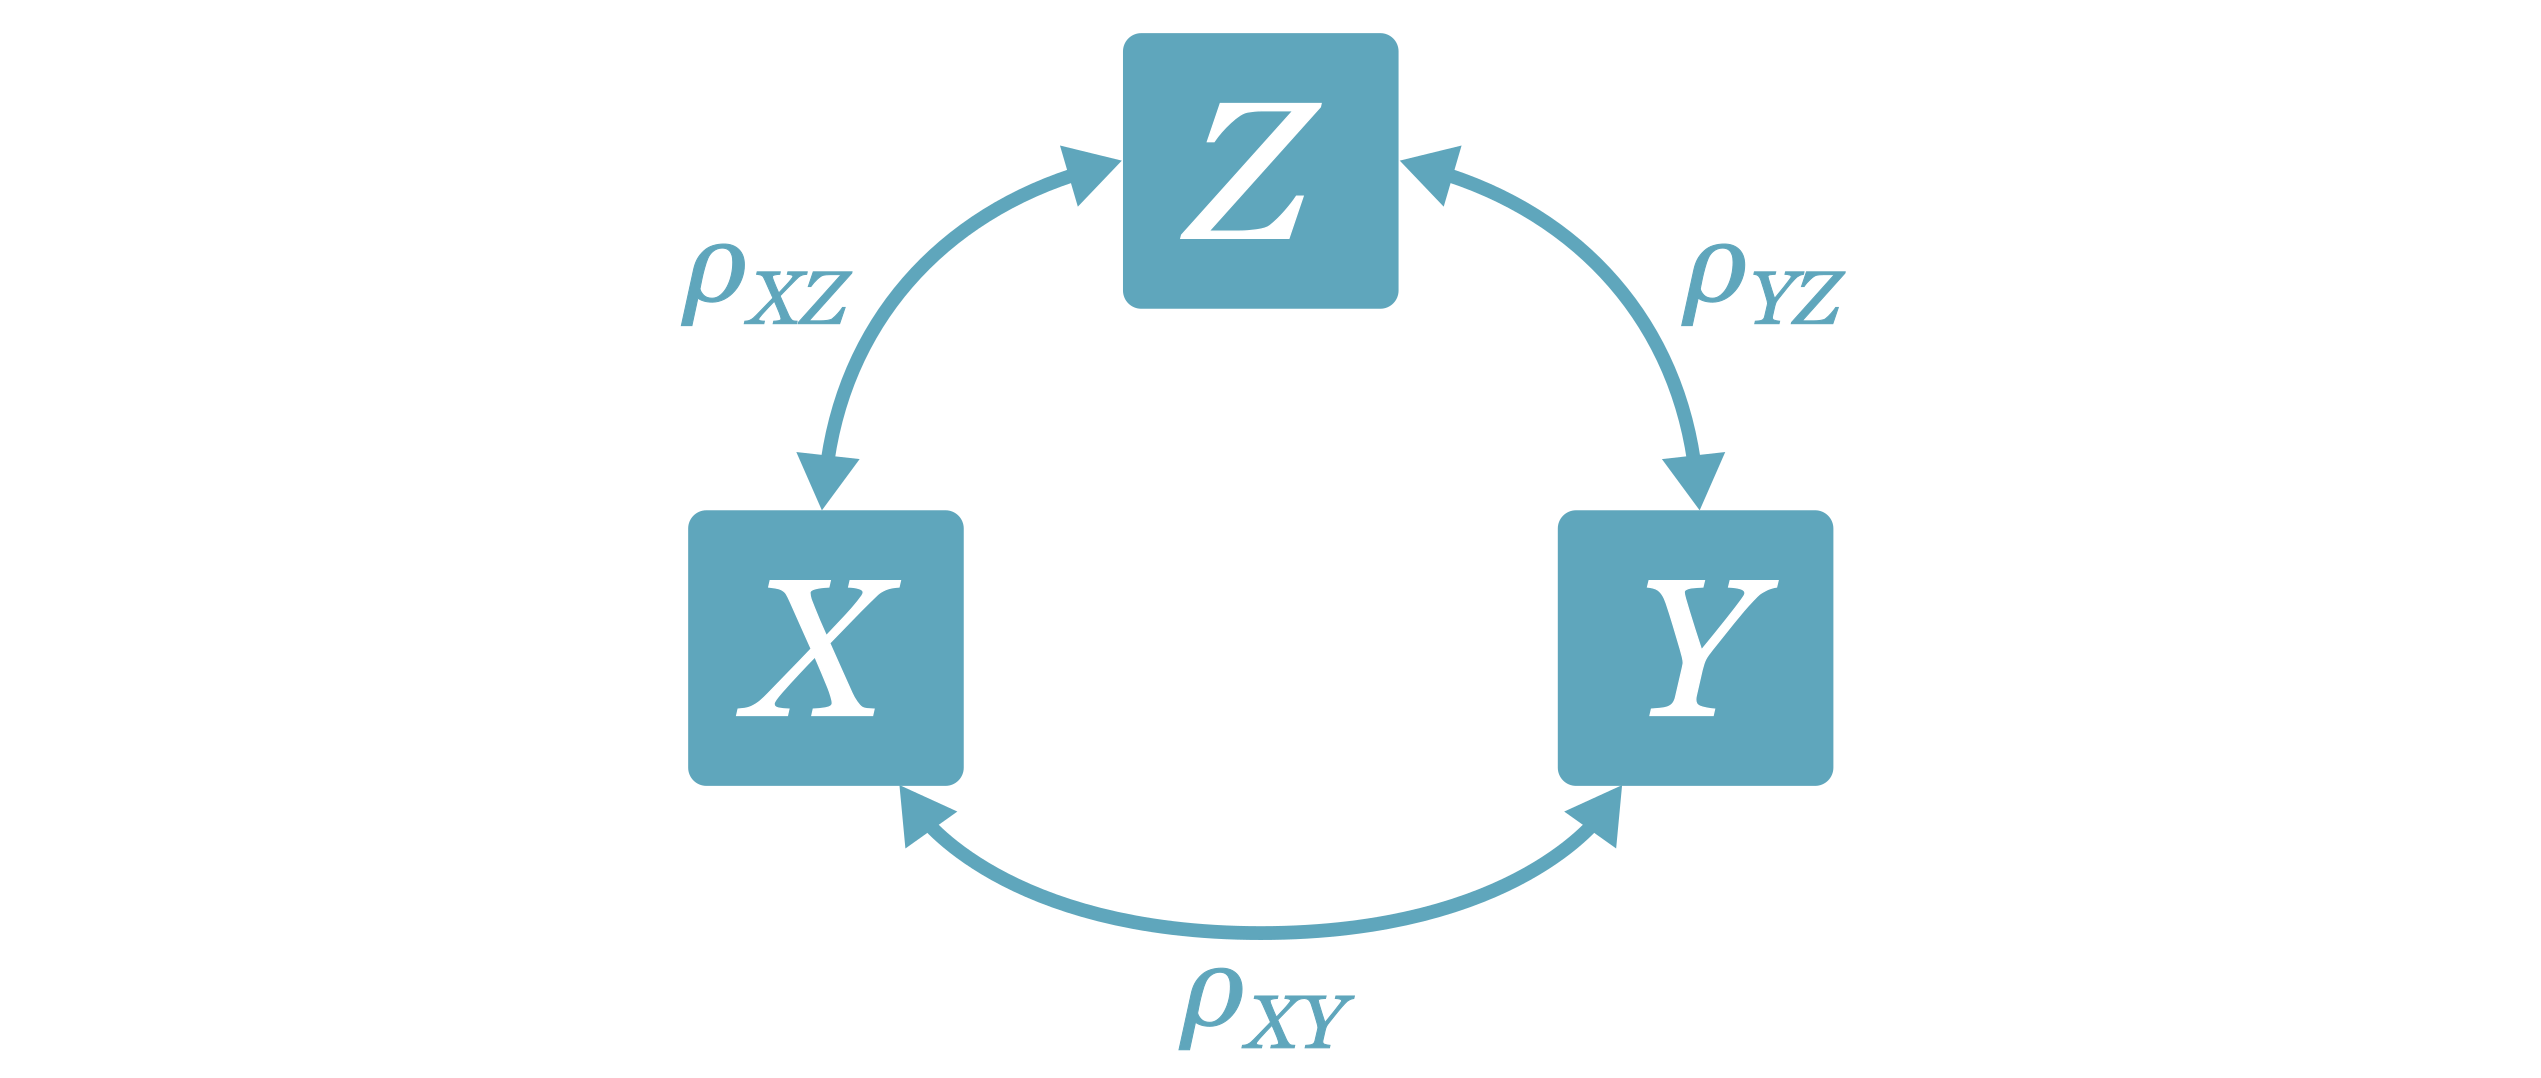
\includegraphics{chapters/10-indirect-selection/figure/indirect_select_corr_model_biv.png}

}

\caption{\label{fig-corr-model-biv}The assumed correlation structure of
univariate indirect selection. The correlation between \(Z\) and \(Y\)
is completely mediated by \(X\) (i.e., the partial correlation between
\(Y\) and \(Z\), controlling for \(X\) is zero such that,
\(\rho_{YZ.X}=0\)).}

\end{figure}%

The scenario displayed in Figure~\ref{fig-bvirr}, shows a \(u\)-ratio of
about \(u_X=u_Y=0.81\) in the independent variable and dependent
variables. We see in the figure below that the correlation in the
restricted sample (\(\rho_{XY|\mathcal{S}(Z)}=.25\)) is attenuated
relative to the target population correlation (\(\rho_{XY}=.50\)).

\begin{figure}[H]

\centering{

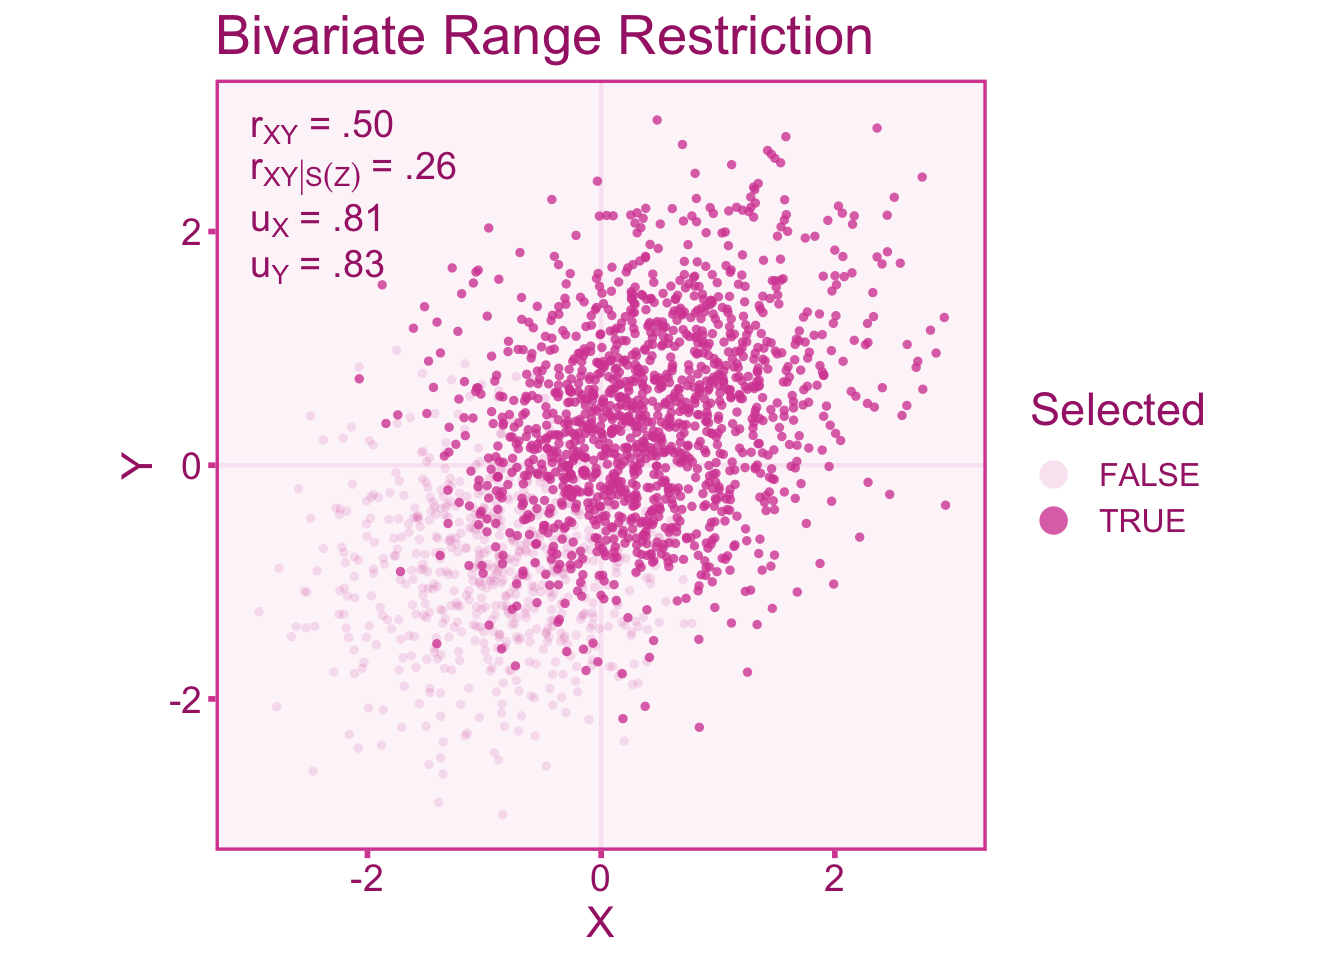
\includegraphics{chapters/10-indirect-selection/10-indirect-selection_files/figure-pdf/fig-bvirr-1.pdf}

}

\caption{\label{fig-bvirr}Scatterplot showing a correlation between
\(X\) and \(Y\) under bivariate indirect range restriction. Dark red
dots indicate the selected sample and the transparent dots indicate the
rejected sample.}

\end{figure}%

Likewise let's visualize what happens to the correlation when the range
is enhanced. Enhancement in both variables can be accomplished by
selecting individuals at the ends of the distribution of \(Z\) (for this
case we will select individuals below a score of -1 and above a score of
1). We can thus define the selection function as,

\[
\mathcal{S}(Z)=\begin{cases} 1 &\text{ if } Z \leq-1 \text{ or } Z \geq 1  \\  0 &\text{ if } Z > -1  \text{ or } Z < 1   \end{cases}
\]

In Figure~\ref{fig-bvire}, we observe an inflation of observed
correlation (\(\rho_{XY|\mathcal{S}(Z)}=.74\)) relative to the target
correlation (\(\rho_{XY}=.50\)). Figure~\ref{fig-bvire} has a
\(u\)-ratio of about \(u_X=u_Y=1.38\) in both the independent variable
and dependent variable.

\begin{figure}[H]

\centering{

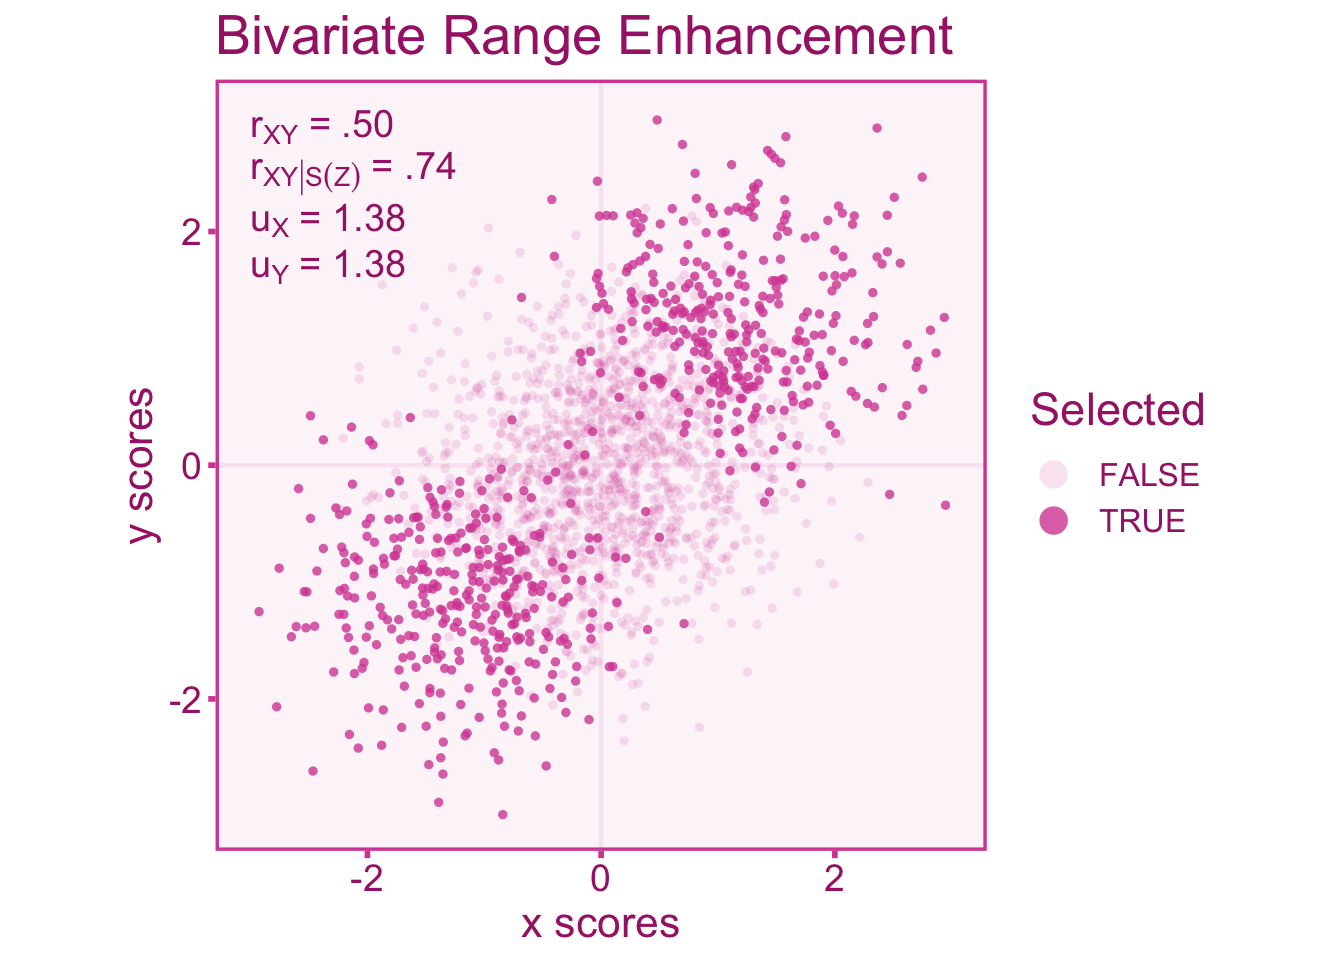
\includegraphics{chapters/10-indirect-selection/10-indirect-selection_files/figure-pdf/fig-bvire-1.pdf}

}

\caption{\label{fig-bvire}Scatterplot showing a correlation between
\(X\) and \(Y\) under bivariate indirect range enhancement. Dark red
dots indicate the selected sample and the transparent dots indicate the
rejected sample.}

\end{figure}%

A bias correction formula for bivariate range restriction is much more
complicated than the univariate formulation. In the univariate case, we
did not need any more information about the selection process beyond
what we could infer from \(u_X\). However in the bivariate case, we need
to have a basic idea of the selection mechanism at play (Dahlke and
Wiernik 2020). Particularly we at least know the direction of the
correlation between the selector variable, \(Z\), and the independent
(\(\rho_{XZ}\)) and dependent variable (\(\rho_{YZ}\)). This will
require a little bit of knowledge about the selection process within a
given study. Let us first define a factor we will denote with
\(\lambda\) (Dahlke and Wiernik 2020). This factor takes into account
the direction of the correlation of \(\rho_{XZ}\) (if positive, we can
set \(\rho_{XZ}=1\), if negative, \(\rho_{XZ}=-1\), if zero,
\(\rho_{XZ}=0\)) and \(\rho_{YZ}\) (repeat the same procedure as
\(\rho_{XZ}\)). Therefore \(\lambda\) can be defined as,

\[\begin{aligned}
\lambda =& \text{ sign}\left(\rho_{XZ}\rho_{YZ} [1-u_X][1-u_Y]\right)\times \\[.3em] &\frac{\text{sign}
\left(1-u_X\right)\min\left(u_X,\frac{1}{u_X}\right) + 
\text{ sign}\left(1-u_Y\right)\min\left(u_Y,\frac{1}{u_Y}\right)
}{\min\left(u_X,\frac{1}{u_X}\right)+\min\left(u_Y,\frac{1}{u_Y}\right)}.
\end{aligned}\]

Although complex, the output of \(\lambda\) will be either -1, 0, or 1.
We can then plug this factor into the full correction equation that
provides us with an unbiased estimate of the correlation in the
unrestricted population,

\[
r_{XY} = r_{XY|\mathcal{S}(Z)}u_Xu_Y+\lambda\sqrt{|1-u_X^2||1-u_Y^2|}
\]

Similar to the univariate formula, we can also incorporate measurement
error into the correction. Measurement error will bias the correlation
on top of the bias induced by range restriction/enhancement. Therefore
we can incorporate the reliabilities estimated within the restricted
sample (\(r_{XX'|\mathcal{S}(Z)}\) and \(r_{YY'|\mathcal{S}(Z)}\)), into
our correction formula:

\[
r_{TU} = \frac{r_{XY|\mathcal{S}(Z)}u_Xu_Y+\lambda\sqrt{|1-u_X^2||1-u_Y^2|}}{\sqrt{1-u_X^2\left(1-r_{XX'|\mathcal{S}(Z)}\right)}\sqrt{1-u_Y^2\left(1-r_{YY'|\mathcal{S}(Z)}\right)}}
\]

If the reliability estimates come from an target population reference
sample, we can get estimates of the reliability coefficients in the
selected sample using Equation~\ref{eq-rel-x} and
Equation~\ref{eq-rel-y}. We then can correct the observed sampling
variance (\(\sigma^2_{\varepsilon_o}\)),

\[
se(r_{TU}) = \frac{se\left(r_{XY|\mathcal{S}(Z)}\right)}{\hat{a}}= \frac{se\left(r_{XY|\mathcal{S}(Z)}\right)}{\left[\frac{r_{XY|\mathcal{S}(Z)}}{r_{TU}}\right]}.
\]

\begin{tcolorbox}[enhanced jigsaw, opacityback=0, coltitle=black, toprule=.15mm, colframe=quarto-callout-note-color-frame, bottomtitle=1mm, rightrule=.15mm, colbacktitle=quarto-callout-note-color!10!white, left=2mm, bottomrule=.15mm, breakable, title={Applied Example in R}, colback=white, opacitybacktitle=0.6, titlerule=0mm, arc=.35mm, leftrule=.75mm, toptitle=1mm]

Continuing with the example from the univariate case, a university
admits applicants based on some criterion upon a composite of multiple
measures of performance (\(Z\)). Two of those measures is a standardized
test (\(X\)) and high school grade-point average (GPA). A researcher
then wants to see how test performance predicts college GPA (\(Y\)).
Since \emph{both} test performance is correlated with the composite used
in the college admissions process, it is likely that we will observe
substantial range restriction in the college sample. The \(u\)-ratio in
test performance and GPA was \(u_{X}=u_{Y}=0.80\) (applicants are the
target population). We also want to correct for measurement error in the
dependent variable (grade-point average) only we use to measure stress,
therefore we obtain a reliability estimate within our sample of
\(r_{YY'|\mathcal{S}(Z)}=.90\). The researcher then conducts the study
and finds a sample correlation of \(r_{XY|\mathcal{S}(Z)}=.25\).

In R, we can correct the correlation by using the \texttt{correct\_r}
function in the \texttt{psychmeta} package (Dahlke and Wiernik 2019).
The \texttt{correction\ =\ \textquotesingle{}uvirr\_x\textquotesingle{}}

\begin{Shaded}
\begin{Highlighting}[]
\FunctionTok{library}\NormalTok{(psychmeta)}

\FunctionTok{correct\_r}\NormalTok{(}\AttributeTok{correction =} \StringTok{\textquotesingle{}uvirr\_x\textquotesingle{}}\NormalTok{,}
          \AttributeTok{rxyi =}\NormalTok{ .}\DecValTok{25}\NormalTok{,  }\CommentTok{\# restricted correlation}
          \AttributeTok{ryy =}\NormalTok{ .}\DecValTok{90}\NormalTok{,  }\CommentTok{\# reliability of GPA}
          \AttributeTok{ux =}\NormalTok{ .}\DecValTok{80}\NormalTok{,   }\CommentTok{\# u ratio of SAT scores}
          \AttributeTok{n =} \DecValTok{100}\NormalTok{)    }\CommentTok{\# sample size}
\end{Highlighting}
\end{Shaded}

\begin{verbatim}
Correlations Corrected for Measurement Error and Univariate Indirect Range Restriction:
---------------------------------------------------------------------------------------
  value CI_LL_95 CI_UL_95   n n_effective
1 0.323   0.0742    0.531 100        58.9
\end{verbatim}

The true score correlation in the target population is estimated to be
\(r_{TU} = .32\, [.07,\, .53]\).

\end{tcolorbox}

\section*{Beware of assumptions}\label{beware-of-assumptions}
\addcontentsline{toc}{section}{Beware of assumptions}

\markright{Beware of assumptions}

Note that these corrections require the following assumptions: 1)
linearity between \(X\) and \(Y\), 2) homoskedasticity, that is, equal
variance in \(Y\) at every level of \(X\).

\bookmarksetup{startatroot}

\chapter{Introduction to Meta-Analysis
Methods}\label{sec-metaanalysis_intro}

\section{Introduction}\label{introduction-8}

Meta-analysis is an analytic tool to synthesize quantitative evidence
from multiple studies. By systematically combining and analyzing the
results of multiple studies, meta-analysis provides a comprehensive
overview, unveiling patterns, trends, and insights that individual
studies might not be able to capture. Combining research findings also
has the added benefit of increasing the precision of our results (i.e.,
greater statistical power). In this section we will cover the method
described by (J. E. Hunter and Schmidt 2015) since it is readily
compatible with artifact corrections (see next chapter). For the
random-effects model however, we use an integrated approach that
incorporates methods from J. E. Hunter and Schmidt (2015) and Hedges and
Vevea (1998) that was first introduced by Morris et al. (2014). However
it is important to note that there are other common methods to conduct
meta-analyses that have their strengths and weaknesses
(\textbf{hedges2014?}; Callender and Osburn 1980; Johnson, Mullen, and
Salas 1995).

\section{Common-Effect Model}\label{common-effect-model}

A common effect model is the simplest form of meta-analysis. It assumes
that all the variation in observed effect sizes is attributable to
sampling error (see Figure~\ref{fig-common-effect}). In other words, all
the observed effect sizes are estimates of the same population effect
size. Note that there is a distinction between \emph{fixed-effects}
models and a \emph{common effect} model (Viechtbauer, n.d.; Laird and
Mosteller 1990). The common effect model assumes that the true effect
size is identical for each study while the fixed effects model does not
assume this. Instead, the fixed effects model can be interpreted as the
weighted average of true effects. Computationally, they are the same and
provide the same parameter estimates, yet the interpretation differs
(Viechtbauer, n.d.).

\begin{figure}[H]

\centering{

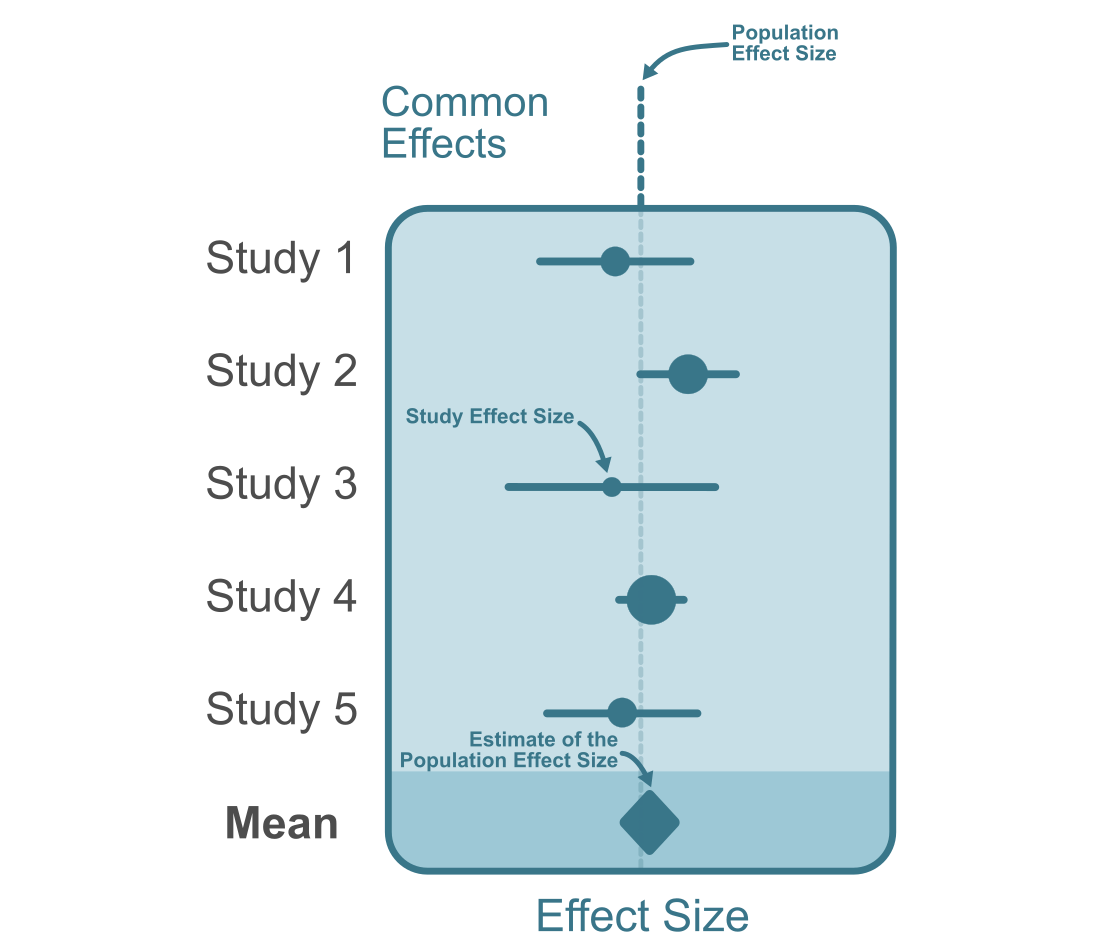
\includegraphics{chapters/11-introduction-to-meta-analysis/figure/fixed_effects_diagram.png}

}

\caption{\label{fig-common-effect}The diagram above depicts a common
effect meta-analysis of five studies. The study effect sizes are
homogenous and all estimate a single true population effect size.}

\end{figure}%

The common effect model can be modeled such that population effect size
\(\theta\) is held constant each study effect size estimate (\(h_i\)),
such that,

\begin{equation}\phantomsection\label{eq-fixed-mdl}{
h_i  = \theta + e_i
}\end{equation}

Where \(e_i\) indicates sampling error and the subscript \(i\) denotes
each study. Similar to the true score theory model that we discussed in
chapter 4, the variance components of each term can similarly be written
out as,

\[
\sigma^2_h = \sigma^2_\theta + \sigma^2_e
\]

However in our common effect model, the population effect size is fixed
across studies and will not vary, simplifying the formula to,

\begin{equation}\phantomsection\label{eq-var-fixed}{
\sigma^2_h = \sigma^2_e
}\end{equation}

Therefore the only source of variation in the observed effect sizes, is
sampling error.

Ultimately, our goal is to obtain a precise estimate of the population
effect size. To obtain an estimate of the population effect size,
\(\theta\), we can calculate the average observed effect size,
\(\bar{h}_i\) from \(k\) studies. However, in practice, effect sizes
from different studies have varying levels of precision (i.e., different
standard errors). A simple arithmetic average will not account for the
differences between studies in their precision. Instead, we can
calculate a weighted average where the weights each study can be
calculated by the inverse variance (i.e., squared standard error) of
each study such that,

\[
w_i = \frac{1}{se(h_i)^2}.
\]

Then we can calculate a weighted average,

\[
\hat{\theta} =\frac{\sum^k_{i=1}w_ih_i}{\sum^k_{i=1}w_i}.
\]

Where \(\sum^k_{i=1}\) is the sum across all \(k\) studies. This
weighted average will be an unbiased estimate of the population effect
size. However, even though this mean effect size is more precise
compared to single-study estimates, it is not exempt from error itself.
We we can compute the standard error for \(\hat{\theta}\) as,

\[
se(\hat{\theta}) = \frac{1}{\sqrt{\sum^k_{i=1} w_i}}
\]

The standard error can be used to compute the 95\% confidence intervals
(if the sampling distribution is approximately normal) of the
meta-analytic point estimate:

\[
CI_{95} = \hat{\theta}\pm 1.96 \cdot se(\hat{\theta})
\]

\begin{tcolorbox}[enhanced jigsaw, opacityback=0, coltitle=black, toprule=.15mm, colframe=quarto-callout-note-color-frame, bottomtitle=1mm, rightrule=.15mm, colbacktitle=quarto-callout-note-color!10!white, left=2mm, bottomrule=.15mm, breakable, title={Applied Example in R}, colback=white, opacitybacktitle=0.6, titlerule=0mm, arc=.35mm, leftrule=.75mm, toptitle=1mm]

Lets use a meta-analytic data set investigating the the effectiveness of
a writing-to-learn intervention on academic achievement from
Bangert-Drowns, Hurley, and Wilkinson (2004). This data set has
standardized mean differences between the treatment group and a control
group from \(k=48\) studies (total sample size: \(n=5,576\)) and is
available within the developmental version of the \texttt{metadat}
package (White et al. 2022). Lets conduct a common effect meta-analysis
using the equations from the previous section. We can use the
\texttt{rma} function in the \texttt{metafor} package (Viechtbauer 2010)
to conduct a common effect
(\texttt{method\ =\ \textquotesingle{}EE\textquotesingle{}})
meta-analysis without having to write each equation by hand.

\begin{Shaded}
\begin{Highlighting}[]
\FunctionTok{library}\NormalTok{(metadat)}
\FunctionTok{library}\NormalTok{(metafor)}

\CommentTok{\# display first 6 studies}
\FunctionTok{head}\NormalTok{(dat.bangertdrowns2004[,}\FunctionTok{c}\NormalTok{(}\StringTok{\textquotesingle{}author\textquotesingle{}}\NormalTok{,}\StringTok{\textquotesingle{}year\textquotesingle{}}\NormalTok{,}\StringTok{\textquotesingle{}ni\textquotesingle{}}\NormalTok{,}\StringTok{\textquotesingle{}yi\textquotesingle{}}\NormalTok{,}\StringTok{\textquotesingle{}vi\textquotesingle{}}\NormalTok{)])}
\end{Highlighting}
\end{Shaded}

\begin{verbatim}

    author year  ni     yi    vi 
1 Ashworth 1992  60  0.650 0.070 
2    Ayers 1993  34 -0.750 0.126 
3   Baisch 1990  95 -0.210 0.042 
4    Baker 1994 209 -0.040 0.019 
5   Bauman 1992 182  0.230 0.022 
6   Becker 1996 462  0.030 0.009 
\end{verbatim}

\begin{Shaded}
\begin{Highlighting}[]
\CommentTok{\# fixed effects model}
\NormalTok{mdl }\OtherTok{\textless{}{-}} \FunctionTok{rma}\NormalTok{(}\AttributeTok{data =}\NormalTok{ dat.bangertdrowns2004,}
           \AttributeTok{yi =}\NormalTok{ yi,}
           \AttributeTok{vi =}\NormalTok{ vi,}
           \AttributeTok{method =} \StringTok{\textquotesingle{}EE\textquotesingle{}}\NormalTok{) }\CommentTok{\# Equal{-}effects = Common Effect}

\CommentTok{\# print results}
\FunctionTok{data.frame}\NormalTok{(}\AttributeTok{theta\_hat =}\NormalTok{ mdl}\SpecialCharTok{$}\NormalTok{b[}\DecValTok{1}\NormalTok{],}
           \AttributeTok{se =}\NormalTok{ mdl}\SpecialCharTok{$}\NormalTok{se[}\DecValTok{1}\NormalTok{],}
           \AttributeTok{CI\_ll =}\NormalTok{ mdl}\SpecialCharTok{$}\NormalTok{ci.lb[}\DecValTok{1}\NormalTok{],}
           \AttributeTok{CI\_ul =}\NormalTok{ mdl}\SpecialCharTok{$}\NormalTok{ci.ub[}\DecValTok{1}\NormalTok{])}
\end{Highlighting}
\end{Shaded}

\begin{verbatim}
  theta_hat         se     CI_ll     CI_ul
1 0.1656264 0.02693136 0.1128419 0.2184109
\end{verbatim}

The results show an estimated population effect of
\(\hat{\theta}=0.17\, [0.11,\, 0.22]\).

\end{tcolorbox}

\section{Random Effects Model}\label{random-effects-model}

The random-effects model refers to a model that allows for the
population effect size to vary from study to study (see
Figure~\ref{fig-random-effects}). Random-effects differs from the fixed
effects model in an important way: it does not assume that all observed
effect sizes come from a single (fixed) population effect size
(Borenstein et al. 2010). This variation in population effect sizes is
called heterogeneity. In the traditional J. E. Hunter and Schmidt (2015)
the weights utilized in the random effects meta-analysis are identical
to the common effect model. In other conventional meta-analysis methods
(Hedges and Vevea 1998), random-effect weights usually include a random
effect component containing the variation in population effect sizes
(this has the effect of making study weights more similar to each other
with more variation in population effects). A modern approach introduced
by Morris et al. (2014) and later tested by Brannick et al. (2019),
added this random effect component to the Hunter-Schmidt method. The
simulation study by Brannick et al. (2019), concluded that weights
incorporating random effect components improved the Hunter-Schmidt
estimates. Here we will discuss Hedges-Vevea's method with some elements
taken from Hunter-Schmidt.

\begin{figure}[H]

\centering{

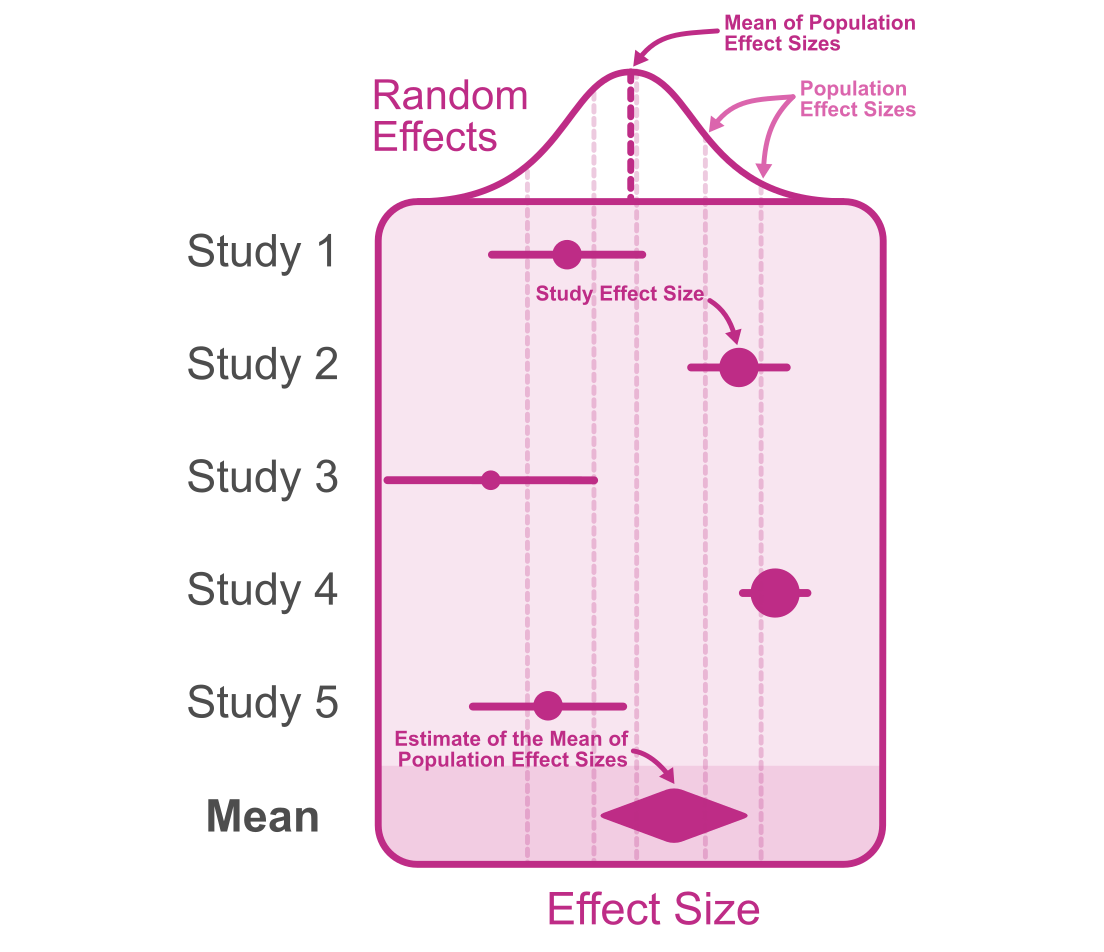
\includegraphics{chapters/11-introduction-to-meta-analysis/figure/random_effects_diagram.png}

}

\caption{\label{fig-random-effects}The diagram above depicts a
random-effects meta-analysis of five studies. Effect sizes are more
variable than the common effect meta-analysis since effect sizes vary
due to sampling error \emph{and} population effect sizes.}

\end{figure}%

The model from Equation~\ref{eq-fixed-mdl} can be changed slightly to
encompass variation of the population effect size from study to study:

\[
h_i = \theta_i + e_i.
\]

In the common effect model, we assumed that all the variation in study
effect sizes is accounted for by variation in sampling error (see
Equation~\ref{eq-var-fixed}). However in the random-effects model the
variance in population effect sizes (\(\sigma^2_\theta\)) is allowed to
be greater than zero. The variance components can be written out as,

\begin{equation}\phantomsection\label{eq-var-random}{
\sigma^2_h=\sigma^2_\theta + \sigma^2_e.
}\end{equation}

Estimating variance components can be done computationally through an
iterative estimation procedure called REstricted Maximum Likelihood
(REML) estimation. The estimated variance of population effect sizes,
\(\hat{\sigma}_\theta\), can now be incorporated into the inverse
variance weights alongside

\[
w_i = \frac{1}{se(h_i)^2 + \hat{\sigma}^2_\theta}
\]

\begin{tcolorbox}[enhanced jigsaw, opacityback=0, coltitle=black, toprule=.15mm, colframe=quarto-callout-tip-color-frame, bottomtitle=1mm, rightrule=.15mm, colbacktitle=quarto-callout-tip-color!10!white, left=2mm, bottomrule=.15mm, breakable, title={Calculating Standard Errors}, colback=white, opacitybacktitle=0.6, titlerule=0mm, arc=.35mm, leftrule=.75mm, toptitle=1mm]

The standard error for a given study often uses the sample estimate in
the sampling variance equation. For example, a study correlation,
\(r_i\), will have a sampling variance of

\[
se(r_i)^2 = \frac{(1-\rho_i^2)^2}{n}
\]

Where \(\rho_i\) is the population effect size for that study. Since the
population effect size is not known, \(\rho_i\) is often replaced with
the study estimate, \(r_i\) (also the denominator will be adjusted to be
\(n-1\) for the decreased degrees of freedom). However this makes the
sampling variances and estimates dependent on one another which can
cause problems for other types analyses (e.g., funnel plot asymmetry).
Instead, we will use the sample size weighted mean correlation for each
study to replace \(\rho_i\) (J. E. Hunter and Schmidt 2015),

\[
se(r_i)^2 = \frac{\left(1-\bar{r}^2\right)^2}{n-1}
\]

Where,

\[
\bar{r} = \frac{\sum^k_{i=1}n_ir_i}{\sum^k_{i=1}n_i}
\]

In studies with no heterogeneity (\(\sigma_\theta=0\)) this is nearly
optimal, but it still works well in cases of substantial heterogeneity.

\end{tcolorbox}

Now we can estimate the mean of population effects by taking the
weighted average effect size (equation 16.5, Cooper, Hedges, and
Valentine 2009),

\[
\hat{\bar{\theta}} = \frac{\sum^k_{i=1}w_i h_i}{\sum^k_{i=1}w_i}.
\]

Where \(i=1...k\) studies. The standard error of the mean of population
effects can calculated from the summation of inverse weights (equation
16.6, Cooper, Hedges, and Valentine 2009),

\[
se(\hat{\bar{\theta}}) = \frac{1}{\sqrt{\sum^k_{i=1}w_i}}.
\] The 95\% confidence interval can then be calculated as,

\[
CI = \hat{\bar{\theta}} \pm 1.96\cdot se(\hat{\bar{\theta}})
\]

In other conventions, the variance in population effects
(\(\sigma^2_\theta\)) is denoted as \(\tau^2\) (Borenstein et al. 2010;
DerSimonian and Kacker 2007; Hedges and Vevea 1998), but conceptually
\(\sigma^2_\theta\) and \(\tau^2\) these are identical. Taking the root
of \(\sigma^2_\theta\) is the standard deviation of population effect
sizes which can be a useful measure of heterogeneity. Furthermore, we
can use \(\hat{\sigma}_\theta\) to calculate credibility (prediction)
intervals which allows us to draw inferences about the range of
plausible population effect sizes. For example, the 90\% credibility
interval can be calculated with the following equations:

\[
CR = \hat{\bar{\theta}} \pm 1.645\hat{\sigma}_\theta
\]

The confidence interval and credibility interval have fundamentally
different interpretations that are often misinterpreted in published
work (Whitener 1990). When we are interpreting a single realized
interval (i.e., our estimate-in-hand), the 90\% \emph{credibility}
interval can be interpreted as the region in which 90\% of population
effect sizes exist, however, a 95\% \emph{confidence} interval describes
the interval in which there is a 95\% probability of containing the true
\emph{mean} of population effect sizes. It is important to note that the
confidence interval interpretation here is only valid in the case of a
single realized interval (Vos and Holbert 2022), if there is more than
one interval obtained from the same population of studies, then the
interpretation does not hold (this would be a rare in a meta-analysis).

\begin{tcolorbox}[enhanced jigsaw, opacityback=0, coltitle=black, toprule=.15mm, colframe=quarto-callout-note-color-frame, bottomtitle=1mm, rightrule=.15mm, colbacktitle=quarto-callout-note-color!10!white, left=2mm, bottomrule=.15mm, breakable, title={Applied Example in R}, colback=white, opacitybacktitle=0.6, titlerule=0mm, arc=.35mm, leftrule=.75mm, toptitle=1mm]

Let's continue looking at the meta-analysis from Bangert-Drowns, Hurley,
and Wilkinson (2004). This data set has standardized mean differences
between the treatment group and a control group from \(k=48\) studies
(total sample size: \(n=5,576\)) and is available within the
developmental version of the \texttt{metadat} package (White et al.
2022). Lets conduct a common effect meta-analysis using the equations
from the previous section. We can use the \texttt{rma} function in the
\texttt{metafor} package (Viechtbauer 2010) to conduct a random effect
meta-analysis with REML estimation we can use the
\texttt{method\ =\ \textquotesingle{}REML\textquotesingle{}} argument.

\begin{Shaded}
\begin{Highlighting}[]
\FunctionTok{library}\NormalTok{(metadat)}
\FunctionTok{library}\NormalTok{(metafor)}

\CommentTok{\# display first 6 studies}
\FunctionTok{head}\NormalTok{(dat.bangertdrowns2004[,}\FunctionTok{c}\NormalTok{(}\StringTok{\textquotesingle{}author\textquotesingle{}}\NormalTok{,}\StringTok{\textquotesingle{}year\textquotesingle{}}\NormalTok{,}\StringTok{\textquotesingle{}ni\textquotesingle{}}\NormalTok{,}\StringTok{\textquotesingle{}yi\textquotesingle{}}\NormalTok{,}\StringTok{\textquotesingle{}vi\textquotesingle{}}\NormalTok{)])}
\end{Highlighting}
\end{Shaded}

\begin{verbatim}

    author year  ni     yi    vi 
1 Ashworth 1992  60  0.650 0.070 
2    Ayers 1993  34 -0.750 0.126 
3   Baisch 1990  95 -0.210 0.042 
4    Baker 1994 209 -0.040 0.019 
5   Bauman 1992 182  0.230 0.022 
6   Becker 1996 462  0.030 0.009 
\end{verbatim}

\begin{Shaded}
\begin{Highlighting}[]
\CommentTok{\# fixed effects model}
\NormalTok{mdl }\OtherTok{\textless{}{-}} \FunctionTok{rma}\NormalTok{(}\AttributeTok{data =}\NormalTok{ dat.bangertdrowns2004,}
           \AttributeTok{yi =}\NormalTok{ yi,}
           \AttributeTok{vi =}\NormalTok{ vi,}
           \AttributeTok{method =} \StringTok{\textquotesingle{}REML\textquotesingle{}}\NormalTok{) }\CommentTok{\# Equal{-}effects = Common Effect}

\CommentTok{\# print results}
\FunctionTok{data.frame}\NormalTok{(}\AttributeTok{theta\_hat =}\NormalTok{ mdl}\SpecialCharTok{$}\NormalTok{b[}\DecValTok{1}\NormalTok{],}
           \AttributeTok{se =}\NormalTok{ mdl}\SpecialCharTok{$}\NormalTok{se[}\DecValTok{1}\NormalTok{],}
           \AttributeTok{CI\_ll =}\NormalTok{ mdl}\SpecialCharTok{$}\NormalTok{ci.lb[}\DecValTok{1}\NormalTok{],}
           \AttributeTok{CI\_ul =}\NormalTok{ mdl}\SpecialCharTok{$}\NormalTok{ci.ub[}\DecValTok{1}\NormalTok{])}
\end{Highlighting}
\end{Shaded}

\begin{verbatim}
  theta_hat         se     CI_ll     CI_ul
1 0.2219296 0.04603453 0.1317036 0.3121556
\end{verbatim}

The results show an estimated population effect of
\(\hat{\theta}=0.22\, [0.13,\, 0.31]\).

\end{tcolorbox}

\bookmarksetup{startatroot}

\chapter{Artifact Correction Meta-Analysis}\label{sec-artifact}

\section{Introduction}\label{introduction-9}

Artifact correction meta-analysis, also referred to as psychometric
meta-analysis, is a form of meta-analysis where effect sizes are
systematically corrected for sources of bias. These sources of bias have
been discussed in previous chapters 4-10. Methodology for conducting
artifact correction style meta-analyses were originally pioneered by
Frank Schmidt and John Hunter (2015; 1977) and then reviewed more
recently by Brenton Wiernik and Jeffrey Dahlke (2020). There has also
been powerful R packages developed to aide in the application of
artifact correction meta-analyses that we have used in previous chapters
(Dahlke and Wiernik 2019). You will notice that in this section, we do
not discuss standardized mean differences. This is due to the fact that
the artifact correction model is designed for pearson correlations, in
order to use this method for standardized mean differences, convert to
pearson correlations using the methods described in chapter 11, and then
use the correction methods used below. Once you apply the corrections to
the converted correlations they can then be converted back to a
standardized mean difference.

\section{Bare Bones vs Artifact Correction
Meta-Analysis}\label{bare-bones-vs-artifact-correction-meta-analysis}

Chapter 11 focused on bare-bones meta-analysis, that is, meta-analyses
that do not correct for biases in effect size estimates. This section
will be dedicated to the artifact correction approach to meta-analysis
that aims to correct for statistical artifacts. The choice between these
two types of meta-analyses depends on the research question, the
available data, and the assumptions researchers are willing to make. If
the goal is to investigate effect sizes as they are reported while
avoiding additional assumptions about the data, then a bare-bones
meta-analysis might be the way to go. On the other hand, if the goal is
to obtain a more accurate estimate of the target effect size by
accounting for biases induced by statistical artifacts, an artifact
correction meta-analysis is preferable.

\begin{enumerate}
\def\labelenumi{\arabic{enumi}.}
\item
  Bare-Bones Meta-Analysis: In a bare-bones meta-analysis, the focus is
  on aggregating effect sizes from various studies without explicitly
  correcting for potential biases in these effect size estimates (see
  first panel of Figure~\ref{fig-art-corr-mdl}).
\item
  Artifact Correction Meta-Analysis: In contrast, an artifact correction
  meta-analysis takes into account and attempts to correct for biases
  that may be present in the effect size estimates from individual
  studies. This involves addressing potential sources of bias, such as
  measurement error or selection effects, through statistical techniques
  or adjustments. By doing so, the meta-analysis aims to provide a more
  accurate and unbiased estimate of the true effect size. Although it is
  important to note that this method will require additional assumptions
  about the nature of the data (see second panel of
  Figure~\ref{fig-art-corr-mdl}).
\end{enumerate}

Note that the bare-bones model does not assume that there is no bias,
rather, the bare-bones model is estimating something else entirely, that
is, the population effect size.

\begin{figure}[H]

\centering{

\captionsetup{labelsep=none}\includegraphics{chapters/12-artifact-correction-meta-analysis/figure/correction_forest.png}

}

\caption{\label{fig-art-corr-mdl}}

\end{figure}%

\section{Individual Artifact Correction
Model}\label{individual-artifact-correction-model}

The individual artifact correction model corrects each effect size
individually prior to conducting the meta-analysis. Let us recall the
random effects model in chapter 11, that an effect size \(h_i\) from
study \(i\) can be modeled such that, \(h_i=\theta_i+e_i\). This model
would be considered a \emph{bare-bones} meta-analytic model. In
practice, observed (study) effect sizes (\(h_i\)) tend to be biased
relative to our target quantity due to many artifacts, some that we can
account for and some we can not. If we decide that corrections to
observed effect sizes are necessary to answer our research question,
then we can construct an artifact correction model. In the artifact
correction model, we can incorporate an artifact attenuation/inflation
factor, \(a\), to the bare-bones formula such that,

\begin{equation}\phantomsection\label{eq-art-mdl}{
h_{i} = a_i\theta_i + e_i
}\end{equation}

The attenuation/inflation factor, \(a_i\), must be estimated for each
study, \(i\). Using estimates of \(a\), Equation~\ref{eq-art-mdl} can be
re-arranged to obtain unbiased estimates of the target population effect
size:

\begin{equation}\phantomsection\label{eq-correction-mdl}{
\frac{h_i}{\hat{a}_i} = \theta_i + \frac{e_i}{\hat{a}_i}
}\end{equation}

This division of \(\hat{a}_i\) will provide us with our corrected effect
size estimates that we can denote with the subscript, \(c\),

\[
h_{c_i} = \frac{h_{i}}{\hat{a}_i}
\]

and of course we must also correct the sampling error term,

\begin{equation}\phantomsection\label{eq-error}{
e_{c_i} = \frac{e_{i}}{\hat{a}_i}.
}\end{equation}

Therefore Equation~\ref{eq-correction-mdl} can be expressed as,

\begin{equation}\phantomsection\label{eq-correction-formula}{
h_{c_i} = \theta_i + e_{c_i} 
}\end{equation}

Like we saw in chapter 11, we can breakdown the variance components of
the model,

\begin{equation}\phantomsection\label{eq-corrected-var}{
\sigma^2_{h_c} = \sigma^2_{\theta} + \sigma^2_{e_c}
}\end{equation}

To obtain these variance components, we can start by correcting the
standard errors from each study. We can calculate the corrected standard
error of the corrected correlations,

\[
se(h_{c_i}) = \frac{se(h_{i})}{\hat{a}_i}
\]

Note that correcting the standard error by dividing by \(\hat{a}\)
ignores any error in the estimation of \(a\) This may also be done by
using the corrected effect size and the observed effect size to correct
the sampling variance:

\[
\sigma^2_{\varepsilon_ci} = \sigma^2_{\varepsilon_oi} \left(\frac{\theta_{c_i}}{\theta_{o_i}}\right)^2
\]

The next step is to obtain the random effects weights of the study, we
can do this with the inverse corrected variance for each study,
\(w_i=1/(\sigma^2_{\varepsilon_ci}+\sigma^2_\rho)\). From here we can
calculate our estimate of the mean of true population correlations,

\[
\hat{\bar{\vartheta}}=\frac{\sum^k_{i=1}n_i\theta_{c_i}}{\sum^k_{i=1}n_i}
\]

Remember that because this is a random effects model,
\(\hat{\bar{\vartheta}}\) is not an estimate of the true population
effect size, instead it is an estimate of the mean of a distribution of
true population effect sizes. Now that we have an estimate of the mean
and the corrected sampling variances, the variance components from
Equation~\ref{eq-corrected-var} can be easily calculated as follows:

\[
\sigma^2_{\theta_c} = \frac{\sum^k_{i=1}n_i(\theta_{c_i} - \hat{\bar{\vartheta}})^2}{\sum^k_{i=1}n_i}
\]

\[
\sigma^2_{\varepsilon_c} = \frac{\sum^k_{i=1}n_i\sigma^2_{\varepsilon_c i}}{\sum^k_{i=1}n_i}
\]

\[
\sigma^2_{\vartheta}  = \sigma^2_{\theta_c} - \sigma^2_{\varepsilon_c}
\]

The standard deviation of true effects is a useful measure of
heterogeneity and is simply the square root of the variance of true
population effect sizes (\(\sigma_{\vartheta}\)). From the standard
deviation in true effects, we can also calculate a credibility
(prediction) interval that shows the range of plausible values for which
a true effect size is likely to fall,

\[
\vartheta_{\text{Upper}} = \hat{\bar{\vartheta}} + 1.645\sigma_\vartheta
\]

\[
\vartheta_{\text{Lower}} = \hat{\bar{\vartheta}} - 1.645\sigma_\vartheta\, .
\]

Note that this is not to be confused with \emph{confidence} intervals
which denotes the range of plausible values that the \emph{mean} of true
effects can take on. This differentiation is akin to understanding the
disparity between the standard error of the mean and the standard
deviation in the context of a normal distribution. We can also see how
the corrections reduced the heterogeneity in the effect size estimates
by comparing variance in true effect sizes (\(\sigma^2_{\vartheta_o}\))
to the variance in observed effect sizes (\(\sigma^2_{\vartheta_o}\);
this can be calculated by conducting a bare-bones random effects
meta-analysis described in chapter 11). The percent reduction in
heterogeneity can be computed by taking the ratio of the two,
\(\sigma^2_{\vartheta}/\sigma^2_{\vartheta_o}\). J. E. Hunter and
Schmidt (2015) suggest that if 75\% of the heterogeneity is accounted
for by artifact corrections, then we can assume that the remaining
heterogeneity is attributable to remaining artifacts that have not been
addressed in the current meta-analysis. Although it is important to
point out that this is simply a rule of thumb rather than a mathematical
property.

\subsection{Individual Corrections in
Correlations}\label{individual-corrections-in-correlations}

For correlation coefficients we can define the model similarly to
Equation~\ref{eq-art-mdl}, with the only difference being that we will
use the notation for pearson correlations,

\[
r_{o_i} = A_i\rho_i + \varepsilon_{o_i}
\]

The artifact correction formulation of this, corresponding to
Equation~\ref{eq-correction-formula}, would be

\[
r_{c_i} = \rho_i + \varepsilon_{c_i}
\]

The corresponding variance components would then be,

\[
\sigma^2_{r_c} = \sigma^2_\rho + \sigma^2_{\varepsilon_c}
\]

In order to compute the variance components as well as the mean true
population correlation, we first need to calculate the study weights. We
will follow a similar procedure for calculating random effects weights
in chapter 11. Lets define the corrected random effects weights as,

\[
w_i = \frac{1}{\sigma^2_{\varepsilon_ci}+\sigma^2_\rho}.
\] However the variance components, \(\sigma^2_{\varepsilon_ci}\) and
\(\sigma^2_\rho\), require the weights themselves to actually estimate
them, so instead we can approximate the variance components using the
sample size as the weights such that,

\[ 
w_i =\frac{1}{\sigma^2_{\varepsilon_ci}+\sigma_\rho^2}= \frac{1}{\sigma^2_{\varepsilon_ci}+(\sigma^2_{r_c}-\sigma^2_{\varepsilon})} \approx \frac{1}{\sigma^2_{\varepsilon_ci}+\left(\frac{\sum^k_{i=1}n_i(r_{c_i} - \bar{r}_c)^2}{\sum^k_{i=1}n_i}-\frac{\sum^k_{i=1}n_i\sigma^2_{\varepsilon_ci}}{\sum^k_{i=1}n_i}\right)} 
\]

Where \(\bar{r}_c\) is the sample size weighted average corrected
correlation. These weights can then be used to obtain a more precise
estimate of the true population correlation,

\[
\hat{\bar{\rho}}=\frac{\sum_{i=1}^k w_i r_{c_i}}{\sum_{i=1}^k w_i}
\] Now we can compute each of the three variance components:

\begin{enumerate}
\def\labelenumi{\arabic{enumi})}
\tightlist
\item
  Variance in corrected correlations:
\end{enumerate}

\[
\sigma^2_{r_c}=\frac{\sum^k_{i=1}w_i(r_{c_i} - \hat{\bar{\rho}})}{\sum^k_{i=1}w_i}.
\] 2) Sampling error variance: \[
\sigma^2_{\varepsilon_c} = \frac{\sum^k_{i=1}w_i\sigma^2_{\varepsilon_ci}}{\sum^k_{i=1}w_i}.
\] 3) Variance in population correlations: \[
\sigma^2_\rho = \sigma^2_r - \sigma^2_{\varepsilon}.
\] Now lets use these variance components to calculate the 90\%
credibility (prediction) interval and the 95\% confidence interval. The
90\% credibility interval can be calculated with the following
equations:

\[
\rho_\text{Upper} = \hat{\bar{\rho}} + 1.645\sigma_\rho
\]

\[
\rho_\text{Lower} = \hat{\bar{\rho}} - 1.645\sigma_\rho
\]

We can also calculate the standard error of the mean of true population
effect sizes (\(SE_{\hat{\bar{\rho}}}\)) by dividing the sampling error
variance component by the number of studies, \(k\),

\[
SE_{\hat{\bar{\rho}}} = \sqrt{\frac{\sigma^2_{r_c}}{k}}
\]

Which can then be used to calculate 95\% confidence intervals:

\[
\bar{\rho}_\text{Upper} = \hat{\bar{\rho}} + 1.96\cdot SE_{\hat{\bar{\rho}}}
\]

\[
\bar{\rho}_\text{Lower} = \hat{\bar{\rho}} - 1.96\cdot SE_{\hat{\bar{\rho}}}
\]

\subsection{Applied Example in R}\label{applied-example-in-r-16}

Lets conduct an individual correction meta-analysis in r using the data
set by Roth (2015). This data set consists of correlations between
school grades and intelligence test scores. It also contains information
on the reliability of the intelligence test scores and the extent of
range restriction in test scores. We can conduct a meta-analysis
correcting for univariate indirect range restriction and measurement
error in test scores. The compound artifact biasing factor for the
correlation would be:

\[
A_i=\sqrt{r_{o_i}^2 + \frac{u_{x_i}^2 r_{xx'_i}(r_{xx'_i} - r_{o_i}^2) }{1 - u_{x_i}^2 (1-r_{xx'_i})} }
\]

Sticking with our theme of doing everything in base R first, lets use
the equations from the previous section to conduct the meta-analysis.

\begin{Shaded}
\begin{Highlighting}[]
\CommentTok{\# Load in packages (we need the development version of psychmeta)}
\CommentTok{\# install.packages("devtools")}
\CommentTok{\# devtools::install\_github("psychmeta/psychmeta")}
\FunctionTok{library}\NormalTok{(psychmeta)}

\CommentTok{\# obtain artifact values}
\NormalTok{rxx }\OtherTok{\textless{}{-}}\NormalTok{ data\_r\_roth\_2015}\SpecialCharTok{$}\NormalTok{rxxi}
\NormalTok{ux }\OtherTok{\textless{}{-}}\NormalTok{ data\_r\_roth\_2015}\SpecialCharTok{$}\NormalTok{ux}
\NormalTok{ro }\OtherTok{\textless{}{-}}\NormalTok{ data\_r\_roth\_2015}\SpecialCharTok{$}\NormalTok{rxyi}
\NormalTok{n }\OtherTok{\textless{}{-}}\NormalTok{ data\_r\_roth\_2015}\SpecialCharTok{$}\NormalTok{n}
\NormalTok{k }\OtherTok{\textless{}{-}} \FunctionTok{length}\NormalTok{(ro)}

\CommentTok{\# fill in missing artifact values with mean}
\NormalTok{rxx[}\FunctionTok{is.na}\NormalTok{(rxx)] }\OtherTok{\textless{}{-}} \FunctionTok{mean}\NormalTok{(rxx,}\AttributeTok{na.rm=}\ConstantTok{TRUE}\NormalTok{)}
\NormalTok{ux[}\FunctionTok{is.na}\NormalTok{(ux)] }\OtherTok{\textless{}{-}} \FunctionTok{mean}\NormalTok{(ux,}\AttributeTok{na.rm=}\ConstantTok{TRUE}\NormalTok{)}

\CommentTok{\# calculate compound artifact biasing factor for univariate direct range restriction with measurement error}
\NormalTok{A }\OtherTok{\textless{}{-}} \FunctionTok{sqrt}\NormalTok{(ro}\SpecialCharTok{\^{}}\DecValTok{2} \SpecialCharTok{+}\NormalTok{ (ux}\SpecialCharTok{\^{}}\DecValTok{2}\SpecialCharTok{*}\NormalTok{rxx}\SpecialCharTok{*}\NormalTok{(rxx }\SpecialCharTok{{-}}\NormalTok{ ro}\SpecialCharTok{\^{}}\DecValTok{2}\NormalTok{)) }\SpecialCharTok{/}\NormalTok{ (}\DecValTok{1} \SpecialCharTok{{-}}\NormalTok{ ux}\SpecialCharTok{\^{}}\DecValTok{2}\SpecialCharTok{*}\NormalTok{(}\DecValTok{1}\SpecialCharTok{{-}}\NormalTok{rxx)))}

\CommentTok{\# calculate the sample size weighted average of r}
\NormalTok{ro\_bar }\OtherTok{\textless{}{-}} \FunctionTok{sum}\NormalTok{(ro}\SpecialCharTok{*}\NormalTok{n) }\SpecialCharTok{/} \FunctionTok{sum}\NormalTok{(n)}

\CommentTok{\# calculate the observed sampling variance for each study}
\NormalTok{var\_eoi }\OtherTok{\textless{}{-}}\NormalTok{ (}\DecValTok{1}\SpecialCharTok{{-}}\NormalTok{ro\_bar}\SpecialCharTok{\^{}}\DecValTok{2}\NormalTok{)}\SpecialCharTok{\^{}}\DecValTok{2} \SpecialCharTok{/}\NormalTok{ (n}\DecValTok{{-}1}\NormalTok{)}

\CommentTok{\# correct sampling variance}
\NormalTok{var\_eci }\OtherTok{\textless{}{-}}\NormalTok{ var\_eoi }\SpecialCharTok{/}\NormalTok{ A}\SpecialCharTok{\^{}}\DecValTok{2}

\CommentTok{\# calculate corrected correlations}
\NormalTok{rc }\OtherTok{\textless{}{-}}\NormalTok{ ro }\SpecialCharTok{/}\NormalTok{ A}

\CommentTok{\# calculate weights}
\NormalTok{w }\OtherTok{\textless{}{-}} \DecValTok{1}\SpecialCharTok{/}\NormalTok{var\_eci}

\CommentTok{\# calculate population effect size estimate}
\NormalTok{mean\_rho\_hat }\OtherTok{\textless{}{-}} \FunctionTok{sum}\NormalTok{(rc}\SpecialCharTok{*}\NormalTok{w) }\SpecialCharTok{/} \FunctionTok{sum}\NormalTok{(w)}

\CommentTok{\# calculate the variance in corrected correlations (rc)}
\NormalTok{var\_rc }\OtherTok{\textless{}{-}} \FunctionTok{sum}\NormalTok{(w}\SpecialCharTok{*}\NormalTok{(rc }\SpecialCharTok{{-}}\NormalTok{ mean\_rho\_hat)}\SpecialCharTok{\^{}}\DecValTok{2}\NormalTok{) }\SpecialCharTok{/} \FunctionTok{sum}\NormalTok{(w)}

\CommentTok{\# calculate average corrected sampling variance}
\NormalTok{var\_ec }\OtherTok{\textless{}{-}} \FunctionTok{sum}\NormalTok{(var\_eci}\SpecialCharTok{*}\NormalTok{w) }\SpecialCharTok{/} \FunctionTok{sum}\NormalTok{(w)}

\CommentTok{\# calculate the variance in true population correlations}
\NormalTok{var\_rho }\OtherTok{\textless{}{-}}\NormalTok{ var\_rc }\SpecialCharTok{{-}}\NormalTok{ var\_ec}

\CommentTok{\# calculate standard error of rho estimate}
\NormalTok{SE\_rho }\OtherTok{=} \FunctionTok{sqrt}\NormalTok{(var\_rc}\SpecialCharTok{/}\NormalTok{k)}

\CommentTok{\# print results}
\FunctionTok{data.frame}\NormalTok{(}\AttributeTok{k =}\NormalTok{ k,}
           \AttributeTok{n =} \FunctionTok{sum}\NormalTok{(n),}
\NormalTok{           mean\_rho\_hat,}
           \AttributeTok{SE =}\NormalTok{ SE\_rho,}
           \AttributeTok{SD\_rho =} \FunctionTok{sqrt}\NormalTok{(var\_rho))}
\end{Highlighting}
\end{Shaded}

\begin{verbatim}
    k      n mean_rho_hat         SE    SD_rho
1 240 105151    0.5398838 0.01339916 0.2022865
\end{verbatim}

The estimated mean correlation of .540 is precisely what is precisely
what the original paper reported (Roth 2015). Lets conduct the
meta-analysis using the the \texttt{psychmeta} package (Dahlke and
Wiernik 2019). The function \texttt{ma\_r\_ic} is designed to conduct an
individual correction meta-analysis on correlation coefficients.

\begin{Shaded}
\begin{Highlighting}[]
\CommentTok{\# install.packages(\textquotesingle{}psychmeta\textquotesingle{})}
\FunctionTok{library}\NormalTok{(psychmeta)}

\CommentTok{\# conduct individual correction meta{-}analysis}
\NormalTok{mdl\_ic }\OtherTok{\textless{}{-}} \FunctionTok{ma\_r\_ic}\NormalTok{(}\AttributeTok{rxyi =}\NormalTok{ ro, }\AttributeTok{n =}\NormalTok{ n,}
            \AttributeTok{correction\_method =} \StringTok{"uvirr"}\NormalTok{,}
            \AttributeTok{rxx =}\NormalTok{ rxx,}
            \AttributeTok{ux =}\NormalTok{ ux,}
            \AttributeTok{ux\_observed =} \ConstantTok{TRUE}\NormalTok{,}
            \AttributeTok{rxx\_restricted =} \ConstantTok{TRUE}\NormalTok{)}

\NormalTok{summary\_stats }\OtherTok{\textless{}{-}} \FunctionTok{data.frame}\NormalTok{(}\AttributeTok{k =}\NormalTok{ mdl\_ic}\SpecialCharTok{$}\NormalTok{meta\_tables}\SpecialCharTok{$}\StringTok{\textasciigrave{}}\AttributeTok{analysis\_id: 1}\StringTok{\textasciigrave{}}\SpecialCharTok{$}\NormalTok{individual\_correction}\SpecialCharTok{$}\NormalTok{true\_score}\SpecialCharTok{$}\NormalTok{k,}
                            \AttributeTok{n =}\NormalTok{ mdl\_ic}\SpecialCharTok{$}\NormalTok{meta\_tables}\SpecialCharTok{$}\StringTok{\textasciigrave{}}\AttributeTok{analysis\_id: 1}\StringTok{\textasciigrave{}}\SpecialCharTok{$}\NormalTok{individual\_correction}\SpecialCharTok{$}\NormalTok{true\_score}\SpecialCharTok{$}\NormalTok{N,}
                            \AttributeTok{mean\_rho =}\NormalTok{ mdl\_ic}\SpecialCharTok{$}\NormalTok{meta\_tables}\SpecialCharTok{$}\StringTok{\textasciigrave{}}\AttributeTok{analysis\_id: 1}\StringTok{\textasciigrave{}}\SpecialCharTok{$}\NormalTok{individual\_correction}\SpecialCharTok{$}\NormalTok{true\_score}\SpecialCharTok{$}\NormalTok{mean\_rho,}
                            \AttributeTok{SE =}\NormalTok{ mdl\_ic}\SpecialCharTok{$}\NormalTok{meta\_tables}\SpecialCharTok{$}\StringTok{\textasciigrave{}}\AttributeTok{analysis\_id: 1}\StringTok{\textasciigrave{}}\SpecialCharTok{$}\NormalTok{individual\_correction}\SpecialCharTok{$}\NormalTok{true\_score}\SpecialCharTok{$}\NormalTok{se\_r\_c,}
                            \AttributeTok{SD\_rho =}\NormalTok{ mdl\_ic}\SpecialCharTok{$}\NormalTok{meta\_tables}\SpecialCharTok{$}\StringTok{\textasciigrave{}}\AttributeTok{analysis\_id: 1}\StringTok{\textasciigrave{}}\SpecialCharTok{$}\NormalTok{individual\_correction}\SpecialCharTok{$}\NormalTok{true\_score}\SpecialCharTok{$}\NormalTok{sd\_rho)}
\NormalTok{summary\_stats }
\end{Highlighting}
\end{Shaded}

\begin{verbatim}
    k      n  mean_rho        SE    SD_rho
1 240 105151 0.5404134 0.0134356 0.2036946
\end{verbatim}

We can also obtain credibility intervals by using the
\texttt{credibility} function in the \texttt{psychmeta} package. The
interval defaults to 80\% intervals, however we can change that to 90\%
by inputting .90 into the \texttt{cred\_level} argument.

\begin{Shaded}
\begin{Highlighting}[]
\FunctionTok{credibility}\NormalTok{(}\AttributeTok{mean =}\NormalTok{ summary\_stats}\SpecialCharTok{$}\NormalTok{mean\_rho\_hat,}
            \AttributeTok{sd =}\NormalTok{ summary\_stats}\SpecialCharTok{$}\NormalTok{SD\_rho,}
            \AttributeTok{cred\_method =} \StringTok{"norm"}\NormalTok{,}
            \AttributeTok{cred\_level =}\NormalTok{ .}\DecValTok{90}\NormalTok{)}
\end{Highlighting}
\end{Shaded}

\begin{verbatim}
     CR_LL_90 CR_UL_90
\end{verbatim}

Lets compare these results to the bare-bones model. In
\texttt{psychmeta} the bare-bones model can be conduced using
\texttt{ma\_r\_bb}. However, the \texttt{ma\_r\_ic} function also
reports the bare-bones results as well. Therefore we can just extract
the necessary statistics from the model.

\begin{Shaded}
\begin{Highlighting}[]
\FunctionTok{data.frame}\NormalTok{(}
  \AttributeTok{k =}\NormalTok{ mdl\_ic}\SpecialCharTok{$}\NormalTok{meta\_tables}\SpecialCharTok{$}\StringTok{\textasciigrave{}}\AttributeTok{analysis\_id: 1}\StringTok{\textasciigrave{}}\SpecialCharTok{$}\NormalTok{barebones}\SpecialCharTok{$}\NormalTok{k,}
  \AttributeTok{n =}\NormalTok{ mdl\_ic}\SpecialCharTok{$}\NormalTok{meta\_tables}\SpecialCharTok{$}\StringTok{\textasciigrave{}}\AttributeTok{analysis\_id: 1}\StringTok{\textasciigrave{}}\SpecialCharTok{$}\NormalTok{barebones}\SpecialCharTok{$}\NormalTok{N,}
  \AttributeTok{mean\_rho\_obs =}\NormalTok{ mdl\_ic}\SpecialCharTok{$}\NormalTok{meta\_tables}\SpecialCharTok{$}\StringTok{\textasciigrave{}}\AttributeTok{analysis\_id: 1}\StringTok{\textasciigrave{}}\SpecialCharTok{$}\NormalTok{barebones}\SpecialCharTok{$}\NormalTok{mean\_r,}
  \AttributeTok{SE =}\NormalTok{ mdl\_ic}\SpecialCharTok{$}\NormalTok{meta\_tables}\SpecialCharTok{$}\StringTok{\textasciigrave{}}\AttributeTok{analysis\_id: 1}\StringTok{\textasciigrave{}}\SpecialCharTok{$}\NormalTok{barebones}\SpecialCharTok{$}\NormalTok{se\_r,}
  \AttributeTok{SD\_rho\_obs =}\NormalTok{ mdl\_ic}\SpecialCharTok{$}\NormalTok{meta\_tables}\SpecialCharTok{$}\StringTok{\textasciigrave{}}\AttributeTok{analysis\_id: 1}\StringTok{\textasciigrave{}}\SpecialCharTok{$}\NormalTok{barebones}\SpecialCharTok{$}\NormalTok{sd\_r)}
\end{Highlighting}
\end{Shaded}

\begin{verbatim}
    k      n mean_rho_obs         SE SD_rho_obs
1 240 105151    0.4418789 0.01191933  0.1846534
\end{verbatim}

We can see that the estimate of the population correlation is largely
attenuated in the observed values. This is due to the fact tests of
intelligence are not perfectly reliable and the scores were restricted
in their range.

\section{Artifact Distribution Model}\label{artifact-distribution-model}

When we observe a lot of missingness in artifact values (e.g., studies
not reporting reliability), we may choose to use an artifact
distribution model. The artifact distribution model conducts a
meta-analysis on the observed effect sizes and artifact values
separately, and then uses the aggregate artifact values to correct for
the observed mean effect size. Since the artifact distribution method
uses Taylor series approximations (Dahlke and Wiernik 2020) that are
custom-tailored to estimate the sampling variance of corrected
correlations, we will skip the general case to focus on its application
to correlations.

\subsection{The Correlational Case}\label{the-correlational-case}

The model here can be broken down into two parts, the first part
aggregates the observed effect sizes and the second part aggregates the
artifact values. The artifact values we will focus on here are the
reliability coefficients (see chapter 5 and 6), however other artifact
values like \(u\)-ratios will follow similar procedures. We can start
with the bare-bones meta-analysis model:
\(r_{o_i} = \rho_{o_i} + \varepsilon_{o_i}\). We can estimate the
observed population correlation (\(\vartheta_{o_i}\)) by first
calculating the weights (using the \(n\)-weighted mean correlation in
the formula for sampling variance, \(\bar{r}\)):

\[
\sigma^2_{\varepsilon_oi} \approx \frac{(1-\bar{r}^2)^2}{n_i-1} 
\]

\[
w_i = \frac{1}{\sigma^2_{\varepsilon_i}+\sigma_\vartheta^2} = \frac{1}{\sigma^2_{\varepsilon_i}+(\sigma^2_{\theta}-\sigma^2_{\varepsilon})} \approx \frac{1}{\sigma^2_{\varepsilon_i}+\left(\frac{\sum^k_{i=1}n_i(\theta_i - \bar{\theta})^2}{\sum^k_{i=1}n_i}-\frac{\sum^k_{i=1}n_i\sigma^2_{\varepsilon_oi}}{\sum^k_{i=1}n_i}\right)}
\]

Taking the mean of the observed study correlations weighted by the
inverse sampling variance,

\[
\hat{\bar{\rho}}_o=\frac{\sum^k_{i=1}w_i r_{o_i}}{\sum^k_{i=1}w_i}
\]

Then lets get the variance in observed population correlations, in order
to do this we need the v

\[
\sigma^2_{\rho_o}=\sigma^2_{r_o} - \sigma^2_{\varepsilon_o} = \frac{\sum^k_{i=1}w_i (r_{o_i}-\hat{\bar{\rho}}_o)^2}{\sum^k_{i=1}w_i} - \frac{\sum^k_{i=1}w_i \sigma^2_{\varepsilon_oi}}{\sum^k_{i=1}w_i}
\]

With the weights we can also take the weighted average of the artifact
values (such as \(u\)-ratios or reliabilities) that are available. For
our example here, we will correct only for measurement error, therefore
the weighted means for reliability in \(x\) and \(y\) will be:

\[
\bar{r}_{xx'}=\frac{\sum^k_{i=1}w_i r_{xx'_i}}{\sum^k_{i=1}w_i}
\]

\[
\bar{r}_{yy'}=\frac{\sum^k_{i=1}w_i r_{yy'_i}}{\sum^k_{i=1}w_i}
\]

Now recall from chapter 5 that the square root of the reliability is
equal to the correlation between observed scores and true scores. We can
denote the mean correlation as follows:
\(\bar{r}_{xT}=\sqrt{\bar{r}_{xx'}}\) and
\(\bar{r}_{yU}=\sqrt{\bar{r}_{xx'}}\). We then must also compute the
average sampling variances of \(r_{xT_i}\) and \(r_{yU_i}\) between
studies. These sampling variance of these correlations can be computed
the same way as a pearson correlation:

\[
\sigma^2_{r_{xT}i} \approx \frac{(1-\bar{r}_{xT}^2)^2}{n_i-1} 
\]

\[
\sigma^2_{r_{yU}i} \approx \frac{(1-\bar{r}_{yU}^2)^2}{n_i-1} 
\]

Then weighted average of these sampling variances is

\[
\sigma^2_{r_{xT}} = \frac{\sum^k_{i=1}w_i r_{xT_i}}{\sum^k_{i=1}w_i}
\]

\[
\sigma^2_{r_{yU}} = \frac{\sum^k_{i=1}w_i r_{yU_i}}{\sum^k_{i=1}w_i}
\]

Now that we have the point-estimate of the population observed
correlation, the variance of observed population correlations, the
sampling variance of observed correlations, and the sampling variance of
the square root of the reliability for \(x\) and \(y\), we can now
attempt to correct the point-estimate and the variance of population
correlations.

\paragraph*{Correcting Using Summary
Values}\label{correcting-using-summary-values}
\addcontentsline{toc}{paragraph}{Correcting Using Summary Values}

First, we can start by correcting the overall point-estimate for the
observed population correlation in order to remove bias due to
measurement error. Recall from chapter 5 the correction formula:

\[
\hat{\bar{\rho}} = \frac{\hat{\bar{\rho}}_o}{\bar{A}} = \frac{\hat{\bar{\rho}}_o}{\bar{r}_{xT} \bar{r}_{yU}} = \frac{\hat{\bar{\rho}}_o}{\sqrt{\bar{r}_{xx'}} \sqrt{\bar{r}_{yy'}}}
\]

Note that the artifact biasing factor, \(A\), is the product of the two
sources of attenuation. Correcting the variance in observed population
correlations (\(\sigma^2_{\rho_o}\)), so that it is accurately
estimating the variance of true population effect sizes
(\(\sigma^2_{\rho}\)), we must use a Taylor series approximation. This
formula can become fairly complex with more types of artifacts involved.
The taylor series approximation is for estimating specifically the
amount of sampling variance within the correction factor we apply to the
observed correlation. The first step is lay out our attenuation formula
(the equation where observed effect size is on the left side of the
equation and the artifact values and true effect size is on the right
hand side of the equation). In the case of correcting only for
measurement error, the attenuation formula is relatively simple

\[
\hat{\bar{\rho}}_o = \hat{\bar{\rho}}\cdot \bar{r}_{xT}\cdot \bar{r}_{yU}
\]

For the taylor series approximation, we want to first find the partial
derivitive with respect to each artifact component:

\[
B_{r_{xT}}=\frac{\partial}{\partial r_{xT}} (\hat{\bar{\rho}}\cdot \bar{r}_{xT}\cdot \bar{r}_{yU}) = \hat{\bar{\rho}}\cdot \bar{r}_{yU}
\] \[
B_{r_{yU}}=\frac{\partial}{\partial r_{yU}} (\hat{\bar{\rho}}\cdot \bar{r}_{xT}\cdot \bar{r}_{yU}) = \hat{\bar{\rho}}\cdot \bar{r}_{xT}
\]

The variance due to artifacts is then approximately,

\[
\sigma^2_A\approx B^2_{r_{xT}} \sigma^2_{r_{xT}} + B^2_{r_{yU}} \sigma^2_{r_{yU}}
\]

Now we can approximate the variance in true population correlations,

\[
\sigma_\rho^2= \frac{\sigma^2_{\rho_o} - \sigma^2_A}{\bar{A}^2}
\]

Where the artifact biasing factor is:
\(\bar{A}=\bar{r}_{xT}\cdot \bar{r}_{yU}\). See the supplementary
materials of Dahlke and Wiernik (2020) for detailed Taylor series
approximation derivations for the immensely more complicated bivariate
indirect range restriction plus measurement error correction.

\subsection{Applied Example in R}\label{applied-example-in-r-17}

Lets conduct an artifact distribution correction meta-analysis in R,
instead using data from the meta-analysis by McDaniel et al. (1994).
This dataset contains correlations between employment interviews and job
performance. This data set has a lot of missing values for reliability
coefficients and \(u\)-ratios which might suggest that the artifact
distribution approach is a better choice compared to the individual
correction approach. We can conduct a meta-analysis correcting for
univariate indirect range restriction and measurement error in both job
performance and employment interviews. The attenuation formula will be
important for calculating the Taylro series approximation can be defined
as

\[
\bar{\rho}_o=\bar{\rho}\sqrt{\bar{r}_{o_i}^2 + \frac{\bar{u}_{x_i}^2 \bar{r}_{xx'_i}(\bar{r}_{xx'_i}\bar{r}_{yy'_i} - \bar{r}_{o_i}^2) }{1 - \bar{u}_{x_i}^2 (1-\bar{r}_{xx'_i})} }
\] Instead of conducting a taylor series approximation by hand, we will
simply use the \texttt{psychmeta} package to perform the artifact
distribution meta-analysis. The function \texttt{ma\_r\_ad} is designed
to conduct an artifact distribution meta-analysis on correlation
coefficients. The function also reports the bare-bones model allowing us
to compare the corrected estimates to the uncorrected.

\begin{Shaded}
\begin{Highlighting}[]
\CommentTok{\# Load in packages (we need the development version of psychmeta)}
\CommentTok{\# install.packages("devtools")}
\CommentTok{\# devtools::install\_github("psychmeta/psychmeta")}
\FunctionTok{library}\NormalTok{(psychmeta)}

\CommentTok{\# obtain artifact values}
\NormalTok{rxx }\OtherTok{\textless{}{-}}\NormalTok{ data\_r\_roth\_2015}\SpecialCharTok{$}\NormalTok{rxxi}
\NormalTok{ux }\OtherTok{\textless{}{-}}\NormalTok{ data\_r\_roth\_2015}\SpecialCharTok{$}\NormalTok{ux}
\NormalTok{ro }\OtherTok{\textless{}{-}}\NormalTok{ data\_r\_roth\_2015}\SpecialCharTok{$}\NormalTok{rxyi}
\NormalTok{n }\OtherTok{\textless{}{-}}\NormalTok{ data\_r\_roth\_2015}\SpecialCharTok{$}\NormalTok{n}
\NormalTok{k }\OtherTok{\textless{}{-}} \FunctionTok{length}\NormalTok{(ro)}

\CommentTok{\# compute barebones meta{-}analysis}
\NormalTok{ma\_obj }\OtherTok{\textless{}{-}} \FunctionTok{ma\_r\_bb}\NormalTok{(}\AttributeTok{r =}\NormalTok{ rxyi, }
                  \AttributeTok{n =}\NormalTok{ n, }
                  \AttributeTok{correct\_bias =} \ConstantTok{FALSE}\NormalTok{, }
                  \AttributeTok{wt\_type =} \StringTok{"REML"}\NormalTok{,}
                  \AttributeTok{data =}\NormalTok{ data\_r\_mcdaniel\_1994)}

\CommentTok{\# construct artifact distribution for x}
\NormalTok{ad\_obj\_x }\OtherTok{\textless{}{-}} \FunctionTok{create\_ad}\NormalTok{(}\AttributeTok{ad\_type =} \StringTok{"tsa"}\NormalTok{, }
                      \AttributeTok{mean\_rxxi =}\NormalTok{ data\_r\_mcdaniel\_1994}\SpecialCharTok{$}\NormalTok{Mrxxi[}\DecValTok{1}\NormalTok{],}
                      \AttributeTok{var\_rxxi =}\NormalTok{ data\_r\_mcdaniel\_1994}\SpecialCharTok{$}\NormalTok{SDrxxi[}\DecValTok{1}\NormalTok{]}\SpecialCharTok{\^{}}\DecValTok{2}\NormalTok{,}
                      \AttributeTok{ux =}\NormalTok{ data\_r\_mcdaniel\_1994}\SpecialCharTok{$}\NormalTok{ux,}
                      \AttributeTok{wt\_ux =}\NormalTok{ data\_r\_mcdaniel\_1994}\SpecialCharTok{$}\StringTok{\textasciigrave{}}\AttributeTok{ux frequency}\StringTok{\textasciigrave{}}\NormalTok{)}

\CommentTok{\# construct artifact distribution for y}
\NormalTok{ad\_obj\_y }\OtherTok{\textless{}{-}} \FunctionTok{create\_ad}\NormalTok{(}\AttributeTok{ad\_type =} \StringTok{"tsa"}\NormalTok{, }
                      \AttributeTok{rxxi =}\NormalTok{ data\_r\_mcdaniel\_1994}\SpecialCharTok{$}\NormalTok{ryyi,}
                      \AttributeTok{wt\_rxxi =}\NormalTok{ data\_r\_mcdaniel\_1994}\SpecialCharTok{$}\StringTok{\textasciigrave{}}\AttributeTok{ryyi frequency}\StringTok{\textasciigrave{}}\NormalTok{)}

\CommentTok{\# compute artifact{-}distribution meta{-}analysis, correcting for measurement error only}
\NormalTok{mdl\_ad }\OtherTok{\textless{}{-}} \FunctionTok{ma\_r\_ad}\NormalTok{(}\AttributeTok{ma\_obj =}\NormalTok{ ma\_obj, }
                  \AttributeTok{ad\_obj\_x =}\NormalTok{ ad\_obj\_x, }
                  \AttributeTok{ad\_obj\_y =}\NormalTok{ ad\_obj\_y, }
                  \AttributeTok{correction\_method =} \StringTok{"meas"}\NormalTok{)}


\CommentTok{\# summary table of meta{-}analysis}
\NormalTok{summary\_stats }\OtherTok{\textless{}{-}} \FunctionTok{data.frame}\NormalTok{(}
  \AttributeTok{type =} \FunctionTok{c}\NormalTok{(}\StringTok{\textquotesingle{}Artifact Distribution\textquotesingle{}}\NormalTok{, }\StringTok{\textquotesingle{}Bare{-}Bones\textquotesingle{}}\NormalTok{),}
  \AttributeTok{k =} \FunctionTok{c}\NormalTok{(mdl\_ad}\SpecialCharTok{$}\NormalTok{meta\_tables}\SpecialCharTok{$}\StringTok{\textasciigrave{}}\AttributeTok{analysis\_id: 1}\StringTok{\textasciigrave{}}\SpecialCharTok{$}\NormalTok{artifact\_distribution}\SpecialCharTok{$}\NormalTok{true\_score}\SpecialCharTok{$}\NormalTok{k,mdl\_ad}\SpecialCharTok{$}\NormalTok{meta\_tables}\SpecialCharTok{$}\StringTok{\textasciigrave{}}\AttributeTok{analysis\_id: 1}\StringTok{\textasciigrave{}}\SpecialCharTok{$}\NormalTok{barebones}\SpecialCharTok{$}\NormalTok{k),}
  \AttributeTok{n =} \FunctionTok{c}\NormalTok{(mdl\_ad}\SpecialCharTok{$}\NormalTok{meta\_tables}\SpecialCharTok{$}\StringTok{\textasciigrave{}}\AttributeTok{analysis\_id: 1}\StringTok{\textasciigrave{}}\SpecialCharTok{$}\NormalTok{artifact\_distribution}\SpecialCharTok{$}\NormalTok{true\_score}\SpecialCharTok{$}\NormalTok{N,mdl\_ad}\SpecialCharTok{$}\NormalTok{meta\_tables}\SpecialCharTok{$}\StringTok{\textasciigrave{}}\AttributeTok{analysis\_id: 1}\StringTok{\textasciigrave{}}\SpecialCharTok{$}\NormalTok{barebones}\SpecialCharTok{$}\NormalTok{N),}
  \AttributeTok{mean\_rho =} \FunctionTok{c}\NormalTok{(mdl\_ad}\SpecialCharTok{$}\NormalTok{meta\_tables}\SpecialCharTok{$}\StringTok{\textasciigrave{}}\AttributeTok{analysis\_id: 1}\StringTok{\textasciigrave{}}\SpecialCharTok{$}\NormalTok{artifact\_distribution}\SpecialCharTok{$}\NormalTok{true\_score}\SpecialCharTok{$}\NormalTok{mean\_rho,mdl\_ad}\SpecialCharTok{$}\NormalTok{meta\_tables}\SpecialCharTok{$}\StringTok{\textasciigrave{}}\AttributeTok{analysis\_id: 1}\StringTok{\textasciigrave{}}\SpecialCharTok{$}\NormalTok{barebones}\SpecialCharTok{$}\NormalTok{mean\_r),}
  \AttributeTok{SE =} \FunctionTok{c}\NormalTok{(mdl\_ad}\SpecialCharTok{$}\NormalTok{meta\_tables}\SpecialCharTok{$}\StringTok{\textasciigrave{}}\AttributeTok{analysis\_id: 1}\StringTok{\textasciigrave{}}\SpecialCharTok{$}\NormalTok{artifact\_distribution}\SpecialCharTok{$}\NormalTok{true\_score}\SpecialCharTok{$}\NormalTok{se\_r\_c,mdl\_ad}\SpecialCharTok{$}\NormalTok{meta\_tables}\SpecialCharTok{$}\StringTok{\textasciigrave{}}\AttributeTok{analysis\_id: 1}\StringTok{\textasciigrave{}}\SpecialCharTok{$}\NormalTok{barebones}\SpecialCharTok{$}\NormalTok{se\_r),}
  \AttributeTok{SD\_rho =} \FunctionTok{c}\NormalTok{(mdl\_ad}\SpecialCharTok{$}\NormalTok{meta\_tables}\SpecialCharTok{$}\StringTok{\textasciigrave{}}\AttributeTok{analysis\_id: 1}\StringTok{\textasciigrave{}}\SpecialCharTok{$}\NormalTok{artifact\_distribution}\SpecialCharTok{$}\NormalTok{true\_score}\SpecialCharTok{$}\NormalTok{sd\_rho,}\DecValTok{0}\NormalTok{))}

\NormalTok{summary\_stats }
\end{Highlighting}
\end{Shaded}

\begin{verbatim}
                   type   k     n  mean_rho         SE    SD_rho
1 Artifact Distribution 160 25244 0.3201828 0.02108407 0.1985571
2            Bare-Bones 160 25244 0.2205043 0.01452023 0.0000000
\end{verbatim}

We can also obtain credibility intervals by using the
\texttt{credibility} function in the \texttt{psychmeta} package. The
interval defaults to 80\% intervals, however we can change that to 90\%
by inputting .90 into the \texttt{cred\_level} argument.

\begin{Shaded}
\begin{Highlighting}[]
\FunctionTok{credibility}\NormalTok{(}\AttributeTok{mean =}\NormalTok{ summary\_stats}\SpecialCharTok{$}\NormalTok{mean\_rho[}\DecValTok{1}\NormalTok{],}
            \AttributeTok{sd =}\NormalTok{ summary\_stats}\SpecialCharTok{$}\NormalTok{SD\_rho[}\DecValTok{1}\NormalTok{],}
            \AttributeTok{cred\_method =} \StringTok{"norm"}\NormalTok{,}
            \AttributeTok{cred\_level =}\NormalTok{ .}\DecValTok{90}\NormalTok{)}
\end{Highlighting}
\end{Shaded}

\begin{verbatim}
         CR_LL_90  CR_UL_90
[1,] -0.006414571 0.6467802
\end{verbatim}

Lets compare these results to the bare-bones model. In
\texttt{psychmeta} the bare-bones model can be conduced using
\texttt{ma\_r\_bb}. However, the \texttt{ma\_r\_ic} function also
reports the bare-bones results as well. Therefore we can just extract
the necessary statistics from the model.

\bookmarksetup{startatroot}

\chapter{Conclusion}\label{conclusion}

\subsubsection*{Future Directions}\label{future-directions}
\addcontentsline{toc}{subsubsection}{Future Directions}

This book is a living resource and it will add new content with each
version. Versions will be released in the
\href{https://github.com/MatthewBJane/artifact-corrections-for-effect-sizes/}{Github
repository} as on the Open Science Framework (\emph{DOI here when
created}). In future releases, there are a number of features that are
planned to be added. Here is a list of those features:

\begin{itemize}
\tightlist
\item
  Interactive visualizations of artifacts and bias using RShinyLive
\item
  More effect size types with corrections: Repeated measures SMDs,
  Variability ratios, and unstandardized effect sizes (mean differences
  and regression coefficients).
\item
  A chapter on the artifact of treatment non-compliance.
\item
  Z-transformations for corrected correlations.
\item
  Practice problems.
\item
  Small simulations for assessing robustness of corrections in
  non-normal distributions (e.g., heavy-tails, skew)
\end{itemize}

Suggestions for added features are welcome. Suggestions can be made by
submitting an issue to the
\href{https://github.com/MatthewBJane/artifact-corrections-for-effect-sizes/}{Github
repository}.

\subsubsection*{Limitations}\label{limitations}
\addcontentsline{toc}{subsubsection}{Limitations}

Applying artifact corrections has trade-offs that should be considered
before putting them into use. Obtaining more accurate estimates of our
target effect sizes is the obvious major benefit of applying
corrections, however it is also true that these artifact corrections can
impose assumptions that may not be met in practice. The assumptions were
laid out in each of the chapters, but it is important for the researcher
to consider how reasonable these assumptions are for their research
context. If the assumption violations are extreme, than the correction
can potentially over- or under-correct the effect size estimates.

Defining the scientific estimand is the most important step before
proceeding with artifact corrections. Each correction procedure is meant
to estimate very specific quantity. If a researcher's target quantity is
different from the one that the correction procedure is trying to
estimate, then the correction may further bias the effect size. A good
example of this is in college admissions testing, where it can be quite
tempting to correct the correlation between test scores and college
grade-point average (GPA) for measurement error in the test scores.
However, the practical utility of test scores is limited to the
prediction capability of observed test scores since admission committees
do not have access to true scores. Therefore if our quantity of interest
is the on-the-ground predictive utility of test scores on GPA, then
correcting the correlation for measurement errors in test scores will
over-estimate the predictive utility. Researchers should ensure that the
ultimate research goals align with the correction procedure.

\subsubsection*{Concluding Remarks}\label{concluding-remarks}
\addcontentsline{toc}{subsubsection}{Concluding Remarks}

Imperfections in studies can obscure our view of reality, inhibit us
from making sense of our observations, and they can mislead us.
Corrections to these imperfections can allow us to see what findings may
look like in an ideal study with perfect conditions. Meta-analyses will
inevitably incorporate imperfect studies that vary in design and
methodology that may restrict our ability to estimate a specific
estimand. However, this should not limit the goal of meta-analysis to be
merely a description of the literature. Corrections can allow
meta-analysts to estimate specific scientifically-relevant quantities.
Donald Rubin (1992) discusses the importance of estimating effect sizes
in theoretically perfect studies:

\begin{quote}
Literature synthesis is fine, but, before scientifically valid
statistical inference can take place, scientifically relevant quantities
(i.e., estimands) must be defined, and the population estimands in the
traditional view may be of limited scientific interest. The
scientifically most interesting estimands involve the hypothetical
results of technically perfect studies, rather than the average of
results from some population of fallible studies.
\end{quote}

Most artifact correction meta-analyses have been conducted almost
exclusively in industrial and organizational psychology (e.g., personnel
selection) and education assessment research (e.g., college admissions
testing). However, the concepts in this book apply to many fields
including biomedical, social science, clinical research, among others.
No discipline is immune to measurement error and selection effects,
therefore it is important to address these artifacts in every field of
research.

This book could not have been accomplished without the pioneering work
of John Hunter and Frank Schmidt. This book stands as a testament to
their foundational contributions to artifact corrections and
meta-analysis. The goal of this current book was to expand the
methodologies and applications presented in their book (J. E. Hunter and
Schmidt 2015). It also aims to provide a comprehensive guide, drawing
upon previous scholarship while adapting to the evolving landscape of
research methodologies.

I hope reading this book will provide invaluable insights and tools that
empower people to address the bias in our studies. May it encourage a
deeper awareness of these issues when confronted with them.

We want our research findings to accurately describe reality. Artifact
corrections help us get closer to that goal.

\subsubsection*{Acknowledgements}\label{acknowledgements}
\addcontentsline{toc}{subsubsection}{Acknowledgements}

Thank you to Dr.~Blair T. Johnson, Dr.~Christopher Rhoads, and
Dr.~Elizabeth Schifano for taking the time to review and provide
extremely valuable feedback over the course of writing this book.

\textbf{\emph{Matthew B. Jané}}

\href{https://x.com/MatthewBJane}{\faIcon{twitter} @MatthewBJane}

\bookmarksetup{startatroot}

\chapter*{References}\label{references}
\addcontentsline{toc}{chapter}{References}

\markboth{References}{References}

\phantomsection\label{refs}
\begin{CSLReferences}{1}{0}
\bibitem[\citeproctext]{ref-aguinis2009}
Aguinis, Herman, Charles A Pierce, and Steven A Culpepper. 2009.
{``Scale Coarseness as a Methodological Artifact,''} September.

\bibitem[\citeproctext]{ref-bangert-drowns2004}
Bangert-Drowns, Robert L, Marlene M Hurley, and Barbara Wilkinson. 2004.
{``The Effects of School-Based Writing-to-Learn Interventions on
Academic Achievement: A Meta-Analysis.''} \emph{Review of Educational
Research} 74 (1): 29--58.
\url{https://doi.org/10.3102/00346543074001029}.

\bibitem[\citeproctext]{ref-barraza2019}
Barraza, Felipe, Marcelo Arancibia, Eva Madrid, and Cristian Papuzinski.
2019. {``General Concepts in Biostatistics and Clinical Epidemiology:
Random Error and Systematic Error.''} \emph{Medwave} 19 (7): e7687.
\url{https://doi.org/10.5867/medwave.2019.07.7687}.

\bibitem[\citeproctext]{ref-bobko1980}
Bobko, Philip, and Angela Rieck. 1980. {``Large Sample Estimators for
Standard Errors of Functions of Correlation Coefficients.''}
\emph{Applied Psychological Measurement} 4 (3): 385--98.
\url{https://doi.org/10.1177/014662168000400309}.

\bibitem[\citeproctext]{ref-bonett2005}
Bonett, Douglas G., and Robert M. Price. 2005. {``Inferential Methods
for the Tetrachoric Correlation Coefficient.''} \emph{Journal of
Educational and Behavioral Statistics} 30 (2): 213--25.
\url{https://www.jstor.org/stable/3701350}.

\bibitem[\citeproctext]{ref-borenstein2010}
Borenstein, Michael, Larry V. Hedges, Julian P. T. Higgins, and Hannah
R. Rothstein. 2010. {``A Basic Introduction to Fixed-Effect and
Random-Effects Models for Meta-Analysis.''} \emph{Research Synthesis
Methods} 1 (2): 97--111. \url{https://doi.org/10.1002/jrsm.12}.

\bibitem[\citeproctext]{ref-borsboom2002}
Borsboom, Denny, and Gideon J Mellenbergh. 2002. {``True Scores, Latent
Variables, and Constructs: A Comment on Schmidt and Hunter.''}

\bibitem[\citeproctext]{ref-borsboom2004}
Borsboom, Denny, Gideon J. Mellenbergh, and Jaap Van Heerden. 2004.
{``The Concept of Validity.''} \emph{Psychological Review} 111 (4):
1061--71. \url{https://doi.org/10.1037/0033-295X.111.4.1061}.

\bibitem[\citeproctext]{ref-brannick2019}
Brannick, Michael T., Sean M. Potter, Bryan Benitez, and Scott B.
Morris. 2019. {``Bias and Precision of Alternate Estimators in
Meta-Analysis: Benefits of Blending Schmidt-Hunter and Hedges
Approaches.''} \emph{Organizational Research Methods} 22 (2): 490--514.
\url{https://doi.org/10.1177/1094428117741966}.

\bibitem[\citeproctext]{ref-bravais1844}
Bravais, A. 1844. \emph{Analyse mathématique sur les probabilités des
erreurs de situation d'un point}. Impr. Royale.

\bibitem[\citeproctext]{ref-brown1910}
Brown, William. 1910. {``Some Experimental Results in the Correlation of
Mental Abilities1.''} \emph{British Journal of Psychology, 1904-1920} 3
(3): 296--322. \url{https://doi.org/10.1111/j.2044-8295.1910.tb00207.x}.

\bibitem[\citeproctext]{ref-callender1980}
Callender, John C., and H. G. Osburn. 1980. {``Development and Test of a
New Model for Validity Generalization.''} \emph{Journal of Applied
Psychology} 65 (5): 543--58.
\url{https://doi.org/10.1037/0021-9010.65.5.543}.

\bibitem[\citeproctext]{ref-cohen1988}
Cohen, Jacob. 1988. \emph{Statistical Power Analysis for the Behavioral
Sciences}. Academic Press.

\bibitem[\citeproctext]{ref-cohen1977}
---------. 2013. \emph{Statistical Power Analysis for the Behavioral
Sciences}. Academic Press.

\bibitem[\citeproctext]{ref-thehand2009}
Cooper, Harris M., Larry V. Hedges, and Jeff C. Valentine, eds. 2009.
\emph{The Handbook of Research Synthesis and Meta-Analysis}. 2nd ed. New
York: Russell Sage Foundation.

\bibitem[\citeproctext]{ref-cox1989}
Cox, D. R. 1989. \emph{Analysis of Binary Data}. 2nd ed. New York:
Routledge. \url{https://doi.org/10.1201/9781315137391}.

\bibitem[\citeproctext]{ref-cronbach1951}
Cronbach, Lee J. 1951. {``Coefficient Alpha and the Internal Structure
of Tests.''} \emph{Psychometrika} 16 (3): 297--334.
\url{https://doi.org/10.1007/BF02310555}.

\bibitem[\citeproctext]{ref-cronbach1955}
Cronbach, Lee J., and Paul E. Meehl. 1955. {``Construct Validity in
Psychological Tests.''} \emph{Psychological Bulletin} 52 (4): 281--302.
\url{https://doi.org/10.1037/h0040957}.

\bibitem[\citeproctext]{ref-dahlke2019}
Dahlke, Jeffrey A., and Brenton M. Wiernik. 2019. {``Psychmeta: An R
Package for Psychometric Meta-Analysis.''} \emph{Applied Psychological
Measurement} 43 (5): 415--16.
\url{https://doi.org/10.1177/0146621618795933}.

\bibitem[\citeproctext]{ref-dahlke2020}
---------. 2020. {``Not Restricted to Selection Research: Accounting for
Indirect Range Restriction in Organizational Research.''}
\emph{Organizational Research Methods} 23 (4): 717--49.
\url{https://doi.org/10.1177/1094428119859398}.

\bibitem[\citeproctext]{ref-dersimonian2007}
DerSimonian, Rebecca, and Raghu N. Kacker. 2007. {``Random-Effects Model
for Meta-Analysis of Clinical Trials: An Update.''} \emph{NIST} 28
(January): 105--14.
\url{https://www.nist.gov/publications/random-effects-model-meta-analysis-clinical-trials-update}.

\bibitem[\citeproctext]{ref-galton1907}
Galton, Francis. 1907. {``Vox Populi.''} \emph{Nature} 75 (1949):
450--51. \url{https://doi.org/10.1038/075450a0}.

\bibitem[\citeproctext]{ref-irr}
Gamer, Matthias, Jim Lemon, Ian Fellows, and Puspendra Singh. 2019.
\emph{Irr: Various Coefficients of Interrater Reliability and
Agreement}. \url{https://CRAN.R-project.org/package=irr}.

\bibitem[\citeproctext]{ref-goulet-pelletier2018}
Goulet-Pelletier, Jean-Christophe, and Denis Cousineau. 2018. {``A
Review of Effect Sizes and Their Confidence Intervals, Part i: The
Cohen{'}s d Family.''} \emph{The Quantitative Methods for Psychology} 14
(4): 242--65. \url{https://doi.org/10.20982/tqmp.14.4.p242}.

\bibitem[\citeproctext]{ref-haddock1998}
Haddock, C. Keith, David Rindskopf, and William R. Shadish. 1998.
{``Using Odds Ratios as Effect Sizes for Meta-Analysis of Dichotomous
Data: A Primer on Methods and Issues.''} \emph{Psychological Methods} 3
(3): 339--53. \url{https://doi.org/10.1037/1082-989X.3.3.339}.

\bibitem[\citeproctext]{ref-haertel2006}
Haertel, Edward H. 2006. {``3. Reliability.''} In, 4th ed.

\bibitem[\citeproctext]{ref-hedges1981}
Hedges, Larry V. 1981. {``Distribution Theory for Glass's Estimator of
Effect Size and Related Estimators.''} \emph{Journal of Educational
Statistics} 6 (2): 107--28.
\url{https://doi.org/10.3102/10769986006002107}.

\bibitem[\citeproctext]{ref-hedges1989}
---------. 1989. {``An Unbiased Correction for Sampling Error in
Validity Generalization Studies.''} \emph{Journal of Applied Psychology}
74 (3): 469--77. \url{https://doi.org/10.1037/0021-9010.74.3.469}.

\bibitem[\citeproctext]{ref-hedges1985}
Hedges, Larry V., and Ingram Olkin. 1985. \emph{Statistical Methods for
Meta-Analysis}. Academic press.
\url{https://books.google.com/books?hl=en&lr=&id=7GviBQAAQBAJ&oi=fnd&pg=PP1&dq=info:e6P1zfh2T6QJ:scholar.google.com&ots=Dx-YqN6_9B&sig=-39HgbYdWPp_BwSTzA9cRODs2Q0}.

\bibitem[\citeproctext]{ref-hedges1998}
Hedges, Larry V., and Jack L. Vevea. 1998. {``Fixed- and Random-Effects
Models in Meta-Analysis.''} \emph{Psychological Methods} 3 (4):
486--504. \url{https://doi.org/10.1037/1082-989X.3.4.486}.

\bibitem[\citeproctext]{ref-holtzman1950}
Holtzman, Wayne H. 1950. {``The Unbiased Estimate of the Population
Variance and Standard Deviation.''} \emph{The American Journal of
Psychology} 63 (4): 615--17. \url{https://doi.org/10.2307/1418879}.

\bibitem[\citeproctext]{ref-hunter1990a}
Hunter, John E., and Frank L. Schmidt. 2015. \emph{Methods of
meta-analysis: correcting error and bias in research findings (third)}.
Third. Thousand Oaks, California: Sage Publications.

\bibitem[\citeproctext]{ref-hunter2006}
Hunter, John E., Frank L. Schmidt, and Huy Le. 2006. {``Implications of
Direct and Indirect Range Restriction for Meta-Analysis Methods and
Findings.''} \emph{Journal of Applied Psychology} 91 (3): 594--612.
\url{https://doi.org/10.1037/0021-9010.91.3.594}.

\bibitem[\citeproctext]{ref-hunter1990}
Hunter, John, and Frank Schmidt. 1990. {``Dichotomization of Continuous
Variables: The Implications for Meta-Analysis.''} \emph{Journal of
Applied Psychology} 75 (June): 334--49.
\url{https://doi.org/10.1037/0021-9010.75.3.334}.

\bibitem[\citeproctext]{ref-jacobs2017}
Jacobs, Perke, and Wolfgang Viechtbauer. 2017. {``Estimation of the
Biserial Correlation and Its Sampling Variance for Use in
Meta-Analysis.''} \emph{Research Synthesis Methods} 8 (2): 161--80.
\url{https://doi.org/10.1002/jrsm.1218}.

\bibitem[\citeproctext]{ref-johnson1995}
Johnson, Blair T., Brian Mullen, and Eduardo Salas. 1995. {``Comparison
of Three Major Meta-Analytic Approaches.''} \emph{Journal of Applied
Psychology} 80 (1): 94--106.
\url{https://doi.org/10.1037/0021-9010.80.1.94}.

\bibitem[\citeproctext]{ref-kelley1927}
Kelley, Truman Lee. 1927. \emph{Interpretation of Educational
Measurements}. World Book Company.

\bibitem[\citeproctext]{ref-vankempen2000}
Kempen, G.m.p. van, and L.j. van Vliet. 2000. {``Mean and Variance of
Ratio Estimators Used in Fluorescence Ratio Imaging.''} \emph{Cytometry}
39 (4): 300--305.
\url{https://doi.org/10.1002/(SICI)1097-0320(20000401)39:4\%3C300::AID-CYTO8\%3E3.0.CO;2-O}.

\bibitem[\citeproctext]{ref-kirk1973}
Kirk, David B. 1973. {``On the Numerical Approximation of the Bivariate
Normal (Tetrachoric) Correlation Coefficient.''} \emph{Psychometrika} 38
(2): 259--68. \url{https://doi.org/10.1007/BF02291118}.

\bibitem[\citeproctext]{ref-kroc2020}
Kroc, Edward, and Bruno D. Zumbo. 2020. {``A Transdisciplinary View of
Measurement Error Models and the Variations of x=t+e.''} \emph{Journal
of Mathematical Psychology} 98 (September): 102372.
\url{https://doi.org/10.1016/j.jmp.2020.102372}.

\bibitem[\citeproctext]{ref-kroenke2003}
Kroenke, Kurt, Robert L. Spitzer, and Janet B. W. Williams. 2003. {``The
Patient Health Questionnaire-2: Validity of a Two-Item Depression
Screener.''} \emph{Medical Care} 41 (11): 1284--92.
\url{https://www.jstor.org/stable/3768417}.

\bibitem[\citeproctext]{ref-laird1990}
Laird, Nan M., and Frederick Mosteller. 1990. {``Some Statistical
Methods for Combining Experimental Results.''} \emph{International
Journal of Technology Assessment in Health Care} 6 (1): 5--30.
\url{https://doi.org/10.1017/S0266462300008916}.

\bibitem[\citeproctext]{ref-le2006}
Le, Huy, and Frank L. Schmidt. 2006. {``Correcting for Indirect Range
Restriction in Meta-Analysis: Testing a New Meta-Analytic Procedure.''}
\emph{Psychological Methods} 11 (4): 416--38.
\url{https://doi.org/10.1037/1082-989X.11.4.416}.

\bibitem[\citeproctext]{ref-lundberg2021}
Lundberg, Ian, Rebecca Johnson, and Brandon M. Stewart. 2021. {``What Is
Your Estimand? Defining the Target Quantity Connects Statistical
Evidence to Theory.''} \emph{American Sociological Review} 86 (3):
532--65. \url{https://doi.org/10.1177/00031224211004187}.

\bibitem[\citeproctext]{ref-maccallum2002}
MacCallum, Robert C., Shaobo Zhang, Kristopher J. Preacher, and Derek D.
Rucker. 2002. {``On the Practice of Dichotomization of Quantitative
Variables.''} \emph{Psychological Methods} 7: 19--40.
\url{https://doi.org/10.1037/1082-989X.7.1.19}.

\bibitem[\citeproctext]{ref-maxwell1993}
Maxwell, Scott, and Harold Delaney. 1993. {``Bivariate Median Splits and
Spurious Statistical Significance.''} \emph{Psychological Bulletin} 113
(January): 181--90. \url{https://doi.org/10.1037/0033-2909.113.1.181}.

\bibitem[\citeproctext]{ref-mcdaniel1994}
McDaniel, Michael A., Deborah L. Whetzel, Frank L. Schmidt, and Steven
D. Maurer. 1994. {``The Validity of Employment Interviews: A
Comprehensive Review and Meta-Analysis.''} \emph{Journal of Applied
Psychology} 79 (4): 599--616.
\url{https://doi.org/10.1037/0021-9010.79.4.599}.

\bibitem[\citeproctext]{ref-mendoza1987}
Mendoza, Jorge L., and Michael Mumford. 1987. {``Corrections for
Attenuation and Range Restriction on the Predictor.''} \emph{Journal of
Educational Statistics} 12 (3): 282--93.
\url{https://doi.org/10.3102/10769986012003282}.

\bibitem[\citeproctext]{ref-morris2014}
Morris, Scott, Rebecca Daisley, Megan Wheeler, and Peggy Boyer. 2014.
{``A Meta-Analysis of the Relationship Between Individual Assessments
and Job Performance.''} \emph{The Journal of Applied Psychology} 100
(May). \url{https://doi.org/10.1037/a0036938}.

\bibitem[\citeproctext]{ref-olkin1958}
Olkin, Ingram, and John W. Pratt. 1958. {``Unbiased Estimation of
Certain Correlation Coefficients.''} \emph{The Annals of Mathematical
Statistics} 29 (1): 201--11. \url{https://www.jstor.org/stable/2237306}.

\bibitem[\citeproctext]{ref-pearson1895}
Pearson, Karl. 1895. {``Notes on the History of Correlation.''}
\emph{Society of Biometricians and Mathematical Statisticians}.
\url{https://doi.org/10.2307/2331722}.

\bibitem[\citeproctext]{ref-pearson1903}
---------. 1903. {``I. Mathematical Contributions to the Theory of
Evolution. {\textemdash}XI. On the Influence of Natural Selection on the
Variability and Correlation of Organs.''} \emph{Philosophical
Transactions of the Royal Society of London. Series A, Containing Papers
of a Mathematical or Physical Character} 200 (321-330): 1--66.
\url{https://doi.org/10.1098/rsta.1903.0001}.

\bibitem[\citeproctext]{ref-pearson1898}
Pearson, Karl, and L. N. G. Filon. 1898. {``Mathematical Contributions
to the Theory of Evolution. IV. On the Probable Errors of Frequency
Constants and on the Influence of Random Selection on Variation and
Correlation. {[}Abstract{]}.''} \emph{Proceedings of the Royal Society
of London} 62: 173--76. \url{https://www.jstor.org/stable/115709}.

\bibitem[\citeproctext]{ref-peters1940}
Peters, Charles C., and Walter R. Van Voorhis. 1940. {``Further Methods
of Correlation.''} In, 362--403. New York, NY, US: McGraw-Hill Book
Company. \url{https://doi.org/10.1037/13596-013}.

\bibitem[\citeproctext]{ref-raju1991}
Raju, Nambury, Michael Burke, Jacques Normand, and George Langlois.
1991. {``A New Meta-Analytic Approach.''} \emph{Journal of Applied
Psychology} 76 (June): 432--46.
\url{https://doi.org/10.1037/0021-9010.76.3.432}.

\bibitem[\citeproctext]{ref-roth2015}
Roth, Bettina. 2015. {``Intelligence and School Grades: A
Meta-Analysis.''}

\bibitem[\citeproctext]{ref-rubin1992}
Rubin, Donald B. 1992. {``Meta-Analysis: Literature Synthesis or
Effect-Size Surface Estimation?''} \emph{Journal of Educational
Statistics} 17 (4): 363--74.
\url{https://doi.org/10.3102/10769986017004363}.

\bibitem[\citeproctext]{ref-sackett2000}
Sackett, Paul R., and Hyuckseung Yang. 2000. {``Correction for Range
Restriction: An Expanded Typology.''} \emph{Journal of Applied
Psychology} 85 (1): 112--18.
\url{https://doi.org/10.1037/0021-9010.85.1.112}.

\bibitem[\citeproctext]{ref-schmidt1977}
Schmidt, Frank, and John Hunter. 1977. {``Development of a General
Solution to the Problem of Validity Generalization.''} \emph{Journal of
Applied Psychology} 62 (October): 529--40.
\url{https://doi.org/10.1037/0021-9010.62.5.529}.

\bibitem[\citeproctext]{ref-soper1914}
Soper, H. E. 1914. {``On the Probable Error of the Bi-Serial Expression
for the Correlation Coefficient.''} \emph{Biometrika} 10 (2/3): 384--90.
\url{https://doi.org/10.2307/2331789}.

\bibitem[\citeproctext]{ref-spearman1904}
Spearman, C. 1904. {``The Proof and Measurement of Association Between
Two Things.''} \emph{International Journal of Epidemiology} 39 (5):
1137--50. \url{https://doi.org/10.1093/ije/dyq191}.

\bibitem[\citeproctext]{ref-spearman1910}
Spearman, Charles. 1910. {``Correlation Calculated from Faulty Data.''}
\emph{British Journal of Psychology} 3 (3): 271295.
\url{https://www.proquest.com/docview/1293688112/citation/7E133DC1091D4E47PQ/1}.

\bibitem[\citeproctext]{ref-marco2021}
Taboga, Marco. 2021. {``Gamma Function.''}
\url{https://www.statlect.com/mathematical-tools/gamma-function}.

\bibitem[\citeproctext]{ref-taylor1976}
Taylor, Erwin K., and Thomas Griess. 1976. {``The Missing Middle in
Validation Research.''} \emph{Personnel Psychology} 29 (1): 5--11.
\url{https://doi.org/10.1111/j.1744-6570.1976.tb00397.x}.

\bibitem[\citeproctext]{ref-viechtbauer2010}
Viechtbauer, Wolfgang. 2010. {``Conducting meta-analyses in R with the
metafor package.''} \emph{Journal of Statistical Software} 36 (3):
1--48. \url{https://doi.org/10.18637/jss.v036.i03}.

\bibitem[\citeproctext]{ref-viechtbauer}
---------. n.d. {``Fixed-Effects and Random-Effects Models in
Meta-Analysis.''} \url{https://wviechtb.github.io/metafor/index.html}.

\bibitem[\citeproctext]{ref-viswesvaran2014}
Viswesvaran, Chockalingam, Deniz S. Ones, Frank L. Schmidt, Huy Le, and
In-Sue Oh. 2014. {``Measurement Error Obfuscates Scientific Knowledge:
Path to Cumulative Knowledge Requires Corrections for Unreliability and
Psychometric Meta-Analyses.''} \emph{Industrial and Organizational
Psychology} 7 (4): 507--18.
\url{https://doi.org/10.1017/S1754942600006799}.

\bibitem[\citeproctext]{ref-vos2022}
Vos, Paul, and Don Holbert. 2022. {``Frequentist Statistical Inference
Without Repeated Sampling.''} \emph{Synthese} 200 (2): 89.
\url{https://doi.org/10.1007/s11229-022-03560-x}.

\bibitem[\citeproctext]{ref-wechsler2008}
Wechsler, David. 2008. \emph{Wechsler Adult Intelligence Scale--Fourth
Edition}. 4th ed. \url{https://doi.org/10.1037/t15169-000}.

\bibitem[\citeproctext]{ref-metadat}
White, Thomas, Daniel Noble, Alistair Senior, W. Kyle Hamilton, and
Wolfgang Viechtbauer. 2022. \emph{Metadat: Meta-Analysis Datasets}.
\url{https://CRAN.R-project.org/package=metadat}.

\bibitem[\citeproctext]{ref-whitener1990}
Whitener, Ellen M. 1990. {``Confusion of Confidence Intervals and
Credibility Intervals in Meta-Analysis.''} \emph{Journal of Applied
Psychology} 75 (3): 315--21.
\url{https://doi.org/10.1037/0021-9010.75.3.315}.

\bibitem[\citeproctext]{ref-wiernik2020}
Wiernik, Brenton M., and Jeffrey A. Dahlke. 2020. {``Obtaining Unbiased
Results in Meta-Analysis: The Importance of Correcting for Statistical
Artifacts.''} \emph{Advances in Methods and Practices in Psychological
Science} 3 (1): 94--123. \url{https://doi.org/10.1177/2515245919885611}.

\bibitem[\citeproctext]{ref-psych}
William Revelle. 2023. \emph{Psych: Procedures for Psychological,
Psychometric, and Personality Research}. Evanston, Illinois:
Northwestern University. \url{https://CRAN.R-project.org/package=psych}.

\bibitem[\citeproctext]{ref-wylie1976}
Wylie, Peter B. 1976. {``Effects of Coarse Grouping and Skewed Marginal
Distributions on the Pearson Product Moment Correlation Coefficient.''}
\emph{Educational and Psychological Measurement} 36 (1): 1--7.
\url{https://doi.org/10.1177/001316447603600101}.

\bibitem[\citeproctext]{ref-zimmerman1975}
Zimmerman, Donald W. 1975. {``Probability Spaces, Hilbert Spaces, and
the Axioms of Test Theory.''} \emph{Psychometrika} 40 (3): 395--412.
\url{https://doi.org/10.1007/BF02291765}.

\end{CSLReferences}



\end{document}
